\documentclass[11pt,oneside,a4paper]{report}

% ---------- course configuration ----------
\def\utplabtotal{8}
\def\utpcoursetitle{Machine Learning}
\def\utpcourseoutline{%
  A step-by-step path through data preparation, shared mathematical
  foundations, supervised and unsupervised learning, and a little touch of
  Deep Learning.%
}

% ---------- everything shared with the other courses ----------
% =====================================================================
%  utpnotes.tex
%  Shared preamble for the UTP teaching-assistant course notes.
%
%  Every book includes this file, and it is the ONLY file a book needs
%  from .shared/: the cover, the logos and the optional diagram
%  libraries are all reached from here. It owns everything the books
%  have in common, so a change here reaches every course at once.
%
%  ------------------------------------------------------------------
%  HOW A COURSE USES THIS FILE
%  ------------------------------------------------------------------
%      \documentclass[11pt,oneside,a4paper]{report}
%
%      \def\utprunninghead{Machine Learning Notes}   % section 1
%      \def\utplabtotal{8}
%      \def\utpcoursetitle{Machine Learning}
%      \def\utpcourseoutline{One or two lines for the cover.}
%
%      % =====================================================================
%  utpnotes.tex
%  Shared preamble for the UTP teaching-assistant course notes.
%
%  Every book includes this file, and it is the ONLY file a book needs
%  from .shared/: the cover, the logos and the optional diagram
%  libraries are all reached from here. It owns everything the books
%  have in common, so a change here reaches every course at once.
%
%  ------------------------------------------------------------------
%  HOW A COURSE USES THIS FILE
%  ------------------------------------------------------------------
%      \documentclass[11pt,oneside,a4paper]{report}
%
%      \def\utprunninghead{Machine Learning Notes}   % section 1
%      \def\utplabtotal{8}
%      \def\utpcoursetitle{Machine Learning}
%      \def\utpcourseoutline{One or two lines for the cover.}
%
%      % =====================================================================
%  utpnotes.tex
%  Shared preamble for the UTP teaching-assistant course notes.
%
%  Every book includes this file, and it is the ONLY file a book needs
%  from .shared/: the cover, the logos and the optional diagram
%  libraries are all reached from here. It owns everything the books
%  have in common, so a change here reaches every course at once.
%
%  ------------------------------------------------------------------
%  HOW A COURSE USES THIS FILE
%  ------------------------------------------------------------------
%      \documentclass[11pt,oneside,a4paper]{report}
%
%      \def\utprunninghead{Machine Learning Notes}   % section 1
%      \def\utplabtotal{8}
%      \def\utpcoursetitle{Machine Learning}
%      \def\utpcourseoutline{One or two lines for the cover.}
%
%      \input{../.shared/utpnotes}
%
%      \utpcontentspage{\small}{\normalsize}{0.65em}{0.07em}{0.16em}
%
%      \begin{document}
%      \utpfrontmatter                     % cover, contents, map
%      \part{Orientation}
%      \input{chapters/01-where-to-begin}
%      \end{document}
%
%  Configuration goes BEFORE the \input; overrides go AFTER it.
%  Paths are relative, so compile from inside the course folder.
%
%  ------------------------------------------------------------------
%  NAMING
%  ------------------------------------------------------------------
%  One name per idea, used by every book. Anything a book can use is
%  either an unprefixed learning box (keyidea, pitfall, labproject,
%  ...) or carries the utp prefix (utpfigure, utptable, utpfig,
%  utpsteps, utppython, UTPNavy, utpcell, ...). Course prefixes such
%  as ml-, ds- or erp- are not used: a chapter moved from one book to
%  another compiles unchanged. .shared/README.md lists every name.
%
%  Adding a new course? Copy .shared/TEMPLATE-main.tex and follow
%  .shared/ADDING-A-COURSE.md. Every step is a numbered checklist.
%
%  ------------------------------------------------------------------
%  CONTENTS
%  ------------------------------------------------------------------
%    1  Course configuration     the knobs a book may set
%    2  Packages                 the shared package set and fonts
%    3  Colour palette           the one UTP palette
%    4  Page layout and tables   margins, lists, table styling
%    5  Table of contents        parts, chapters, labs, figures
%    6  Headings                 chapter badge, part pages, sections
%    7  Page furniture           running heads and footers
%    8  Learning boxes           key idea, pitfall, try it, and friends
%    9  Small commands           \term, \cmd, \chapterguide, utpsteps
%   10  Diagram node styles      the TikZ vocabulary every book shares
%   11  Figure frames            utpfigure, utpfig, source images
%   12  Lab sheets               the lab banner and the lab toolkit
%   13  Stage divider            the part-opening page in longer books
%   14  Front matter             \utpfrontmatter: cover, contents, map
%   15  Listing styles           code, terminal and pseudocode
% =====================================================================

% --------------------------------------------------------------------
%  1.  COURSE CONFIGURATION
% --------------------------------------------------------------------
%  The knobs below, plus \utpstyleparts in section 5 and the box titles
%  in section 8, are the whole configuration surface. A book sets what
%  it needs BEFORE the \input and inherits the rest.
%
%  \providecommand means "define unless the book already did", which is
%  what makes the \def-before-\input pattern work.
%
%  Running text
%    \utprunninghead   the left running head on every page.
%    \utpchapterlabel  the word in the chapter badge. CHAPTER by
%                      default; a book whose chapters are labs sets LAB.
%    \utplabtotal      the N in the "Lab 3 of N" banners.

\providecommand{\utprunninghead}{Course Notes}
\providecommand{\utpchapterlabel}{CHAPTER}
\providecommand{\utplabtotal}{10}

%  Cover, printed by section 14
%    \utpcoursetitle       the title on the title page.
%    \utpdocumentsubtitle  the line under the title; Teaching Assistant Guide by default.
%    \utpcourseoutline     the sentence or two below it; \\ breaks a line.
%    \utpoutlineheading    the small heading above that sentence.
%    \utpauthor            the name in the PREPARED BY block.
%    \utpauthorrole        the line under the name.

\providecommand{\utpcoursetitle}{\utprunninghead}
\providecommand{\utpdocumentsubtitle}{Teaching Assistant Guide}
\providecommand{\utpcourseoutline}{}
\providecommand{\utpoutlineheading}{COURSE OUTLINE}
\providecommand{\utpauthor}{Reeyan Afzal Khan}
\providecommand{\utpauthorrole}{Graduate Research Assistant}

%  Files and folders
%    \utpextragraphicspath  image folders to search before the standard
%                           ones, as brace groups: {{screenshots/}}.
%                           A course's own figures/ folder and the
%                           shared logos are always searched.
%    \utpcoursemap          the overview chapter \utpfrontmatter inputs
%                           after the contents. Empty means none.

\providecommand{\utpextragraphicspath}{}
\providecommand{\utpcoursemap}{chapters/course-map}

%  Contents entries for chapters (section 5 applies them). A book whose
%  chapters are labs says so once here rather than restating the three
%  tocloft settings after the input.
%    \utpchaptertocword      Chapter~ by default, Lab~ in one book.
%    \utpchaptertocindent    left indent of the entry.
%    \utpchaptertocnumwidth  room reserved for the word and number.

\providecommand{\utpchaptertocword}{Chapter~}
\providecommand{\utpchaptertocindent}{1.5em}
\providecommand{\utpchaptertocnumwidth}{6em}

%  Monospace face (section 2)
%    \utpmonofont   sourcecodepro by default. inconsolata is the
%                   alternative, for a book whose pages are mostly
%                   device transcripts.

\providecommand{\utpmonofont}{sourcecodepro}

% --------------------------------------------------------------------
%  2.  PACKAGES
% --------------------------------------------------------------------
%  The union of what the books need. A course that needs something
%  extra loads it in its own file, under the heading "packages only
%  this book needs". Pseudocode is the one optional package the shared
%  file knows about: \utpusealgorithms in section 15 loads and styles it.
%
%  The tikz and pgfplots library lists are the union across all books,
%  so a diagram or chart copied from one course compiles in another.

\usepackage[T1]{fontenc}
\IfFileExists{glyphtounicode.tex}{\input{glyphtounicode}\pdfgentounicode=1}{}
\usepackage[american]{babel}
\IfFileExists{sourcesanspro.sty}
  {\usepackage[default]{sourcesanspro}}
  {\usepackage[scaled]{helvet}\renewcommand{\familydefault}{\sfdefault}}
\DeclareFontShape{T1}{cmss}{b}{n}{<->ssub*cmss/bx/n}{}
\DeclareFontShape{TS1}{cmss}{b}{n}{<->ssub*cmss/bx/n}{}
% Monospace. Without this the tt default stays Computer Modern Typewriter,
% a serif face that clashes with the sans body text in every listing and
% every \cmd. Source Code Pro is the companion to Source Sans Pro; it is
% scaled down because mono digits otherwise sit large next to the sans.
%
% Inconsolata, chosen with \def\utpmonofont{inconsolata}, distinguishes
% 0/O and 1/l/I at a glance, which matters when a reader copies an
% interface name or an address out of a transcript. Only one mono package
% is ever loaded: a second would win the family but inherit the first's
% series names, and every \ttfamily would then resolve by substitution.
\def\utpmonoinconsolata{inconsolata}
\ifx\utpmonofont\utpmonoinconsolata
  \IfFileExists{inconsolata.sty}{\usepackage[varqu,varl,scaled=1.02]{inconsolata}}{}
\else
  \IfFileExists{sourcecodepro.sty}
    {\usepackage[scaled=0.88]{sourcecodepro}}
    {\usepackage[scaled=0.86]{beramono}}
  % Source Sans names its normal weight "regular", but the Computer Modern
  % fallbacks call it "m". Map one onto the other so a \ttfamily reached
  % while the regular series is active resolves instead of warning.
  \DeclareFontShape{T1}{cmtt}{regular}{n}{<->ssub*cmtt/m/n}{}
  \DeclareFontShape{TS1}{cmtt}{regular}{n}{<->ssub*cmtt/m/n}{}
  \DeclareFontShape{T1}{cmtt}{regular}{it}{<->ssub*cmtt/m/it}{}
\fi
\usepackage[margin=21mm,headheight=22pt]{geometry}
\usepackage{amsmath,amssymb,mathtools,bm}
\usepackage{microtype}
\usepackage{enumitem}
\usepackage{booktabs}
\usepackage{tabularx}
\usepackage{array}
\usepackage{ragged2e}
\usepackage{etoolbox}
\usepackage{titlesec}
\usepackage{tocloft}
\usepackage{fancyhdr}
\usepackage[table]{xcolor}
\usepackage{tcolorbox}
\tcbuselibrary{breakable,skins}
\usepackage[hidelinks]{hyperref}
\usepackage{bookmark}
% Document properties, so the PDF identifies itself in a reader's
% title bar, in a library catalogue, and in search results. Set from
% the same configuration macros the cover uses.
\hypersetup{
  pdftitle={\utpcoursetitle},
  pdfauthor={\utpauthor},
  pdfsubject={Universiti Teknologi PETRONAS course notes and laboratory guide},
  pdfkeywords={UTP, course notes, laboratory manual, \utpcoursetitle},
  pdfdisplaydoctitle=true,
  bookmarksnumbered=true,
  bookmarksopenlevel=1
}
\usepackage{listings}
\usepackage{graphicx}
\usepackage{caption}
\usepackage{tikz}
\usetikzlibrary{angles,arrows.meta,backgrounds,calc,chains,decorations.pathmorphing,decorations.pathreplacing,fit,matrix,patterns,positioning,quotes,shadows.blur,shapes.geometric,shapes.misc,shapes.symbols}
\usepackage{pgfplots}
% statistics gives boxplot prepared; groupplots gives multi-panel charts.
\usepgfplotslibrary{statistics}
\usepgfplotslibrary{groupplots}

% Images: any folders the book names first, then its own figures/
% folder, then the shared logos used by the cover.
\expandafter\graphicspath\expandafter{\utpextragraphicspath{figures/}{../.shared/logos/}}

% --------------------------------------------------------------------
%  3.  COLOUR PALETTE
% --------------------------------------------------------------------
%  One palette, defined once under UTP* names, and used by every book,
%  box, diagram and chart. Five accents (blue, teal, green, orange, red)
%  with a pale tint of each for box backgrounds, plus navy for headings,
%  gold for the cover, ink and muted for text, and a sixth accent,
%  purple, for charts and layered diagrams that need one more series.

\definecolor{UTPNavy}{HTML}{18324A}
\definecolor{UTPBlue}{HTML}{246B9E}
\definecolor{UTPTeal}{HTML}{138A80}
\definecolor{UTPGreen}{HTML}{2D7D46}
\definecolor{UTPOrange}{HTML}{C86B24}
\definecolor{UTPRed}{HTML}{B34843}
\definecolor{UTPPurple}{HTML}{6B4FA0}
\definecolor{UTPGold}{HTML}{D4A13E}
\definecolor{UTPInk}{HTML}{263238}
\definecolor{UTPMuted}{HTML}{60717C}
\definecolor{UTPPaleBlue}{HTML}{EEF6FB}
\definecolor{UTPPaleTeal}{HTML}{EEF8F6}
\definecolor{UTPPaleOrange}{HTML}{FFF5EA}
\definecolor{UTPPaleRed}{HTML}{FFF0EF}
\definecolor{UTPPalePurple}{HTML}{F0ECF9}
\definecolor{UTPPaleGray}{HTML}{F4F6F7}
\color{UTPInk}

% --------------------------------------------------------------------
%  4.  PAGE LAYOUT AND TABLES
% --------------------------------------------------------------------
%  Paragraph spacing, list indents, and the table look: alternating
%  row tint, top-aligned paragraph columns, ragged-right cells.
%
%  Two extra column types for tabularx tables:
%      D{width}   a fixed-width, ragged-right, vertically centred column
%      Y          a ragged-right column that fills the remaining width
%
%  Every table in every book has the same shape, the one Algorithms &
%  Data Structures set: a utptable frame around a full-width tabularx,
%  booktabs rules, a tinted header row of \utpth cells (centred, bold,
%  navy), and a first column in bold navy when it names the rows.
%  Cells are vertically centred, so use m{} rather than p{} columns.
%
%      \begin{utptable}
%      \begin{tabularx}{\linewidth}{@{}>{\bfseries\leavevmode\color{UTPNavy}}m{0.22\linewidth}X@{}}
%      \toprule
%      \rowcolor{UTPPaleBlue!92}
%      \utpth{Operation} & \utpth{What it does} \\
%      \midrule
%      Insertion & Add a new element. \\
%      \bottomrule
%      \end{tabularx}
%      \end{utptable}
%
%  A book whose tables carry dense text asks for \utpcompacttables after
%  the input: tabularx tables then set in \footnotesize with tighter
%  padding and vertically centred cells.

\setlength{\parindent}{0pt}
\setlength{\parskip}{0.55em}
\setlist[itemize]{leftmargin=1.45em,itemsep=0.22em,topsep=0.25em}
\setlist[enumerate]{leftmargin=1.75em,itemsep=0.28em,topsep=0.3em}
\setlist[description]{font=\bfseries\color{UTPNavy},itemsep=0.25em,topsep=0.3em}
\renewcommand{\arraystretch}{1.34}
\setlength{\tabcolsep}{6.5pt}
\arrayrulecolor{UTPBlue!45}
% Keep paragraph-style columns ragged and vertically centred. Tables use
% fixed m columns beside flexible X columns; giving X the same centring
% keeps a short cell level with a tall neighbour in a multi-line row.
\renewcommand{\tabularxcolumn}[1]{m{#1}}
\makeatletter
\g@addto@macro\@arrayparboxrestore{\RaggedRight\arraybackslash}
\makeatother
% A header cell: centred, bold and navy, on the tinted header row.
\newcommand{\utpth}[1]{\multicolumn{1}{c}{\bfseries\color{UTPNavy}#1}}
\AtBeginEnvironment{tabular}{\small\setlength{\extrarowheight}{0.6pt}\rowcolors{2}{UTPPaleBlue!72}{white}}
\AtBeginEnvironment{tabularx}{\small\setlength{\extrarowheight}{0.6pt}\rowcolors{2}{UTPPaleBlue!72}{white}}
\AtBeginEnvironment{figure}{\centering}
\newcolumntype{D}[1]{>{\raggedright\arraybackslash}m{#1}}
\newcolumntype{Y}{>{\raggedright\arraybackslash}X}
\newcommand{\utpcompacttables}{%
  \renewcommand{\tabularxcolumn}[1]{m{##1}}%
  \AtBeginEnvironment{tabularx}{%
    \footnotesize
    \setlength{\tabcolsep}{4pt}%
    \renewcommand{\arraystretch}{1.25}%
    \setlength{\extrarowheight}{0.6pt}%
  }%
}
\emergencystretch=1.5em
\hbadness=10000
\hfuzz=8pt

% Page-breaking discipline. Without these a paragraph can leave a single
% line stranded at the foot of one page or the head of the next, which is
% the most visible sign of unattended typesetting.
\widowpenalty=10000          % no first line of a paragraph left alone at a page foot
\clubpenalty=10000           % no last line of a paragraph left alone at a page head
\displaywidowpenalty=10000   % the same around displayed equations
\brokenpenalty=10000         % do not break a page after a hyphenated line
\predisplaypenalty=10000     % keep the line before a display with it
% Pages are built from boxes of many heights, so let the last line float
% up rather than stretching the gaps between boxes to force a flush foot.
\raggedbottom
% Prefer a slightly loose line to an overfull one, but do not hyphenate
% freely -- short sans lines look ragged when over-hyphenated.
\tolerance=1200
\hyphenpenalty=200

% Character protrusion and font expansion. Both are what stop a justified
% sans column from showing visible rivers down the page.
\microtypesetup{protrusion=true,expansion=true,tracking=true}

\pgfplotsset{
  compat=1.18,
  every axis/.append style={
    axis line style={draw=UTPMuted!85,line width=0.55pt},
    tick style={draw=UTPMuted!85},
    tick label style={font=\scriptsize\color{UTPMuted}},
    label style={font=\small\color{UTPNavy}},
    title style={font=\small\bfseries\color{UTPNavy}},
    legend style={font=\scriptsize,draw=UTPBlue!22,fill=white,rounded corners=1pt}
  },
  every axis plot/.append style={line width=1.15pt}
}
\tikzset{every picture/.append style={line cap=round,line join=round}}

% --------------------------------------------------------------------
%  5.  TABLE OF CONTENTS
% --------------------------------------------------------------------
%  Formatting for part, chapter and lab entries, and for a list of
%  figures if a book prints one. The lab level is a custom tocloft list
%  so lab banners appear in the contents.
%
%  Part styling is skipped when \utpstyleparts is 0, which is what a
%  book without \part divisions should set.
%
%  The contents page is meant to fill exactly one page, and how loosely
%  it is set depends on how many entries a book has. One line after the
%  input tunes it:
%
%      \utpcontentspage{<base size>}{<part size>}%
%                      {<space before a part>}{<before a chapter>}{<before a lab>}
%      \utpcontentspage{\normalsize}{\large}{1.15em}{0.38em}{0.30em}   % the default

\addto\captionsamerican{\renewcommand{\contentsname}{Learning Path}}
\newlistentry{lab}{toc}{-1}
\providecommand{\utpstyleparts}{1}
\ifnum\utpstyleparts=1
\renewcommand{\cftpartpresnum}{}
\renewcommand{\cftpartaftersnum}{}
\setlength{\cftpartnumwidth}{5.2em}
\setlength{\cftbeforepartskip}{0.38em}
\renewcommand{\cftpartfont}{\normalsize\bfseries\color{UTPNavy}}
\renewcommand{\cftpartpagefont}{\normalsize\bfseries\color{UTPNavy}}
\renewcommand{\cftpartleader}{\hfill}
\fi
\renewcommand{\cftchappresnum}{\utpchaptertocword}
\renewcommand{\cftchapaftersnum}{\quad}
\setlength{\cftchapindent}{\utpchaptertocindent}
\setlength{\cftchapnumwidth}{\utpchaptertocnumwidth}
\setlength{\cftbeforechapskip}{0pt}
\renewcommand{\cftchapfont}{\normalfont}
\renewcommand{\cftchappagefont}{\normalfont}
\renewcommand{\cftchapleader}{\cftdotfill{\cftdotsep}}
\setlength{\cftlabindent}{3em}
\setlength{\cftlabnumwidth}{0em}
\setlength{\cftbeforelabskip}{0.10em}
\renewcommand{\cftlabfont}{\bfseries\color{UTPOrange!90!black}}
\renewcommand{\cftlabpagefont}{\bfseries\color{UTPOrange!90!black}}
\renewcommand{\cftlableader}{\color{UTPOrange!65!UTPMuted}\cftdotfill{\cftlabdotsep}}

% A list of figures, for a book that prints one (\listoffigures).
\renewcommand{\cftfigfont}{\normalfont\small}
\renewcommand{\cftfigpagefont}{\normalfont\small}
\renewcommand{\cftfigpresnum}{Figure~}
\renewcommand{\cftfigaftersnum}{\quad}
\setlength{\cftfigindent}{1.5em}
\setlength{\cftfignumwidth}{5.6em}
\setlength{\cftbeforefigskip}{0pt}
\renewcommand{\cftfigleader}{\cftdotfill{\cftdotsep}}

% The contents page itself, printed by \utpfrontmatter (section 14).
\newcommand{\utpcontentspage}[5]{%
  \def\utptocsize{#1}\def\utptocpartsize{#2}%
  \def\utptocpartskip{#3}\def\utptocchapterskip{#4}\def\utptoclabskip{#5}}
\utpcontentspage{\normalsize}{\large}{1.15em}{0.38em}{0.30em}
\newcommand{\utptableofcontents}{%
  \begingroup
  \utptocsize
  \setlength{\parskip}{0pt}%
  \setlength{\cftbeforepartskip}{\utptocpartskip}%
  \setlength{\cftbeforechapskip}{\utptocchapterskip}%
  \setlength{\cftbeforelabskip}{\utptoclabskip}%
  \renewcommand{\cftpartfont}{\utptocpartsize\bfseries\color{UTPNavy}}%
  \renewcommand{\cftpartpagefont}{\utptocpartsize\bfseries\color{UTPNavy}}%
  \tableofcontents
  \endgroup
}

% --------------------------------------------------------------------
%  6.  HEADINGS
% --------------------------------------------------------------------
%  The chapter badge (a coloured block with a word and the number),
%  part pages, and section spacing.
%
%  The word in the badge is \utpchapterlabel; Data Communication sets
%  it to LAB because each of its chapters is a lab.

\titleformat{\chapter}[display]
  {\bfseries\color{UTPNavy}}
  {\filleft\colorbox{UTPBlue}{\parbox{2.55cm}{\centering\color{white}\Large
    \utpchapterlabel\\[-0.15em]\Huge\thechapter}}}
  {0.65em}{\Huge\raggedright}
  [\vspace{0.25em}{\color{UTPBlue}\titlerule[1.2pt]}]
\renewcommand{\thepart}{Stage~\arabic{part}}
\titleformat{\part}[display]
  {\centering\color{UTPNavy}\bfseries}
  {\Large\color{UTPTeal}\thepart}{0.45em}{\Huge}
  [\vspace{0.55em}\color{UTPTeal}\rule{0.45\linewidth}{1.5pt}]
\titleformat{\section}{\Large\bfseries\color{UTPNavy}}{\thesection}{0.55em}{}
\titleformat{\subsection}{\large\bfseries\color{UTPBlue}}{\thesubsection}{0.5em}{}
\titlespacing*{\chapter}{0pt}{-1.8em}{1.0em}
\titlespacing*{\part}{0pt}{0pt}{1em}
\titlespacing*{\section}{0pt}{1.2em}{0.35em}
\titlespacing*{\subsection}{0pt}{0.95em}{0.2em}

% --------------------------------------------------------------------
%  7.  PAGE FURNITURE
% --------------------------------------------------------------------
%  Running heads and footers. The left header is \utprunninghead;
%  the right one follows the current chapter.

\pagestyle{fancy}
\fancyhf{}
\lhead{\small\color{UTPMuted}\utprunninghead}
\rhead{\small\color{UTPMuted}\nouppercase{\leftmark}}
\cfoot{\small\color{UTPMuted}\thepage}
\renewcommand{\headrulewidth}{0.5pt}
\renewcommand{\headrule}{\hbox to\headwidth{\color{UTPPaleBlue}\leaders\hrule height \headrulewidth\hfill}}
\renewcommand{\chaptermark}[1]{\markboth{#1}{}}
\fancypagestyle{plain}{%
  \fancyhf{}%
  \cfoot{\small\color{UTPMuted}\thepage}%
  \renewcommand{\headrulewidth}{0pt}%
}

% --------------------------------------------------------------------
%  8.  LEARNING BOXES
% --------------------------------------------------------------------
%  The coloured callouts the chapters use. Every title is a macro, so
%  a book can rename a box without restating its geometry:
%
%      \def\utptitlepitfall{Technical note}   % before the input
%
%  To change how a box LOOKS in one book, use one of the named
%  variations at the end of this section, or \renewtcolorbox after the
%  input. To add a box only one book needs, declare it in that book
%  with \utpnewcallout or \utpnewquietbox.

% Box titles -- override any of these before the input line.
\providecommand{\utptitlekeyidea}{Key idea}
\providecommand{\utptitleworked}{Worked example}
\providecommand{\utptitlepitfall}{Common mistake}
\providecommand{\utptitletryit}{Try it yourself}
\providecommand{\utptitlequickcheck}{Check your understanding}
\providecommand{\utptitlerecap}{Chapter recap}
\providecommand{\utptitledeliverable}{Lab deliverable}
\providecommand{\utptitlelabmode}{How much is scaffolded?}
\providecommand{\utptitleintuition}{Plain idea}
\providecommand{\utptitlefirstread}{Core path}
\providecommand{\utptitleglance}{Chapter at a glance}
\providecommand{\utptitledebug}{Debugging task}
\providecommand{\utptitleoptional}{Beyond the core}
\providecommand{\utptitleverification}{Verification checklist}
\providecommand{\utptitletroubleshoot}{Troubleshooting}
\providecommand{\utptitlesourcebasis}{Source basis}

% Explaining an idea
\newtcolorbox{keyidea}{enhanced,breakable,colback=UTPPaleTeal,colframe=UTPTeal, boxrule=0.8pt,arc=2mm,left=2.5mm,right=2.5mm,top=1.8mm,bottom=1.8mm, fonttitle=\bfseries\color{UTPNavy},title=\utptitlekeyidea}
\newtcolorbox{workedexample}{enhanced,breakable,colback=UTPPaleBlue,colframe=UTPBlue, boxrule=0.8pt,arc=2mm,left=2.5mm,right=2.5mm,top=1.8mm,bottom=1.8mm, fonttitle=\bfseries\color{UTPNavy},title=\utptitleworked}
\newtcolorbox{pitfall}{enhanced,breakable,colback=UTPPaleRed,colframe=UTPRed, boxrule=0.8pt,arc=2mm,left=2.5mm,right=2.5mm,top=1.8mm,bottom=1.8mm, fonttitle=\bfseries\color{UTPNavy},title=\utptitlepitfall}
% Asking the reader to do something
\newtcolorbox{tryit}{enhanced,breakable,colback=white,colframe=UTPTeal, boxrule=0.9pt,arc=2mm,left=2.5mm,right=2.5mm,top=1.8mm,bottom=1.8mm, fonttitle=\bfseries\color{white},colbacktitle=UTPTeal,title=\utptitletryit}
\newtcolorbox{quickcheck}{enhanced,breakable,colback=white,colframe=UTPOrange, boxrule=0.9pt,arc=2mm,left=2.5mm,right=2.5mm,top=1.8mm,bottom=1.8mm, fonttitle=\bfseries\color{white},colbacktitle=UTPOrange,title=\utptitlequickcheck}
\newtcolorbox{chapterrecap}{enhanced,breakable,colback=UTPPaleTeal,colframe=UTPGreen, boxrule=0.9pt,arc=2mm,left=2.5mm,right=2.5mm,top=1.8mm,bottom=1.8mm, fonttitle=\bfseries\color{white},colbacktitle=UTPGreen,title=\utptitlerecap}
% Lab structure
\newtcolorbox{labdeliverable}{enhanced,breakable,colback=white,colframe=UTPGreen, boxrule=0.9pt,arc=2mm,left=2.6mm,right=2.6mm,top=1.9mm,bottom=1.9mm, fonttitle=\bfseries\color{white},colbacktitle=UTPGreen,title=\utptitledeliverable}
\newtcolorbox{labmode}{enhanced,breakable,colback=UTPPaleBlue!52,colframe=UTPBlue, boxrule=0.75pt,arc=2mm,left=2.6mm,right=2.6mm,top=1.7mm,bottom=1.7mm, fonttitle=\bfseries\color{white},colbacktitle=UTPBlue,title=\utptitlelabmode}
% Softer, lighter-weight asides
\newtcolorbox{intuition}{enhanced,breakable,colback=white,colframe=UTPOrange!42, boxrule=0.5pt,arc=2mm,left=2.5mm,right=2.5mm,top=1.5mm,bottom=1.5mm, fonttitle=\bfseries\color{UTPOrange!85!black},title=\utptitleintuition}
\newtcolorbox{firstread}{enhanced,breakable,colback=white,colframe=UTPBlue!42, boxrule=0.5pt,arc=2mm,left=2.5mm,right=2.5mm,top=1.5mm,bottom=1.5mm, fonttitle=\bfseries\color{UTPBlue}, title=\utptitlefirstread}
\newtcolorbox{debugtask}{enhanced,breakable,colback=UTPPaleRed!58,colframe=UTPRed, boxrule=0.85pt,arc=2mm,left=2.6mm,right=2.6mm,top=1.9mm,bottom=1.9mm, fonttitle=\bfseries\color{white},colbacktitle=UTPRed,title=\utptitledebug}
\newtcolorbox{analogy}{enhanced,breakable,colback=white,colframe=UTPOrange!38, boxrule=0.5pt,arc=2mm,left=2.5mm,right=2.5mm,top=1.5mm,bottom=1.5mm, fonttitle=\bfseries\color{UTPOrange!85!black},title=Analogy}
\newtcolorbox{coursechoice}{enhanced,breakable,colback=white,colframe=UTPNavy, boxrule=0.8pt,arc=2mm,left=2.8mm,right=2.8mm,top=2mm,bottom=2mm, fonttitle=\bfseries\color{white},colbacktitle=UTPNavy,title=Course choice}
\newtcolorbox{decisionmemo}{enhanced,breakable,colback=UTPPaleOrange!55,colframe=UTPOrange, boxrule=0.85pt,arc=2mm,left=2.6mm,right=2.6mm,top=1.9mm,bottom=1.9mm, fonttitle=\bfseries\color{white},colbacktitle=UTPOrange,title=Decision memo}
\newtcolorbox{libnote}{enhanced,breakable,colback=white,colframe=UTPMuted!48, boxrule=0.5pt,arc=2mm,left=2.5mm,right=2.5mm,top=1.5mm,bottom=1.5mm, fonttitle=\bfseries\color{UTPNavy},title=Reference note}
\newtcolorbox{miniproject}{enhanced,breakable,colback=UTPPaleTeal!52,colframe=UTPGreen, boxrule=0.9pt,arc=2mm,left=2.6mm,right=2.6mm,top=1.9mm,bottom=1.9mm, fonttitle=\bfseries\color{white},colbacktitle=UTPGreen,title=Mini-project}
% Where the material came from: the lecturer's slides, manual or tutorial
% that a chapter is built on.
\newtcolorbox{sourcebasis}{enhanced,breakable,colback=white,colframe=UTPMuted!55, boxrule=0.5pt,arc=2mm,left=2.5mm,right=2.5mm,top=1.5mm,bottom=1.5mm, fonttitle=\bfseries\color{UTPMuted},title=\utptitlesourcebasis}
% Boxes that take a title argument
\newtcolorbox{modelcard}[1]{enhanced,breakable,colback=white,colframe=UTPBlue, boxrule=0.9pt,arc=2mm,left=2.5mm,right=2.5mm,top=1.8mm,bottom=1.8mm, fonttitle=\bfseries\color{white},colbacktitle=UTPBlue,title=#1}
\newtcolorbox{optionaltopic}{enhanced,breakable,colback=white,colframe=UTPMuted!58, boxrule=0.5pt,arc=2mm,left=2.5mm,right=2.5mm,top=1.5mm,bottom=1.5mm, fonttitle=\bfseries\color{UTPMuted},title=\utptitleoptional}
\newtcolorbox{secondpass}{enhanced,breakable,colback=UTPPaleGray!82,colframe=UTPMuted, boxrule=0.75pt,arc=2mm,left=2.6mm,right=2.6mm,top=1.9mm,bottom=1.9mm, fonttitle=\bfseries\color{white},colbacktitle=UTPMuted,title=Second pass}
\newtcolorbox{labproject}[1]{enhanced,breakable,colback=white,colframe=UTPBlue, boxrule=0.9pt,arc=2mm,left=2.6mm,right=2.6mm,top=1.9mm,bottom=1.9mm, fonttitle=\bfseries\color{white},colbacktitle=UTPBlue,title={#1}}
% Evidence that a lab worked, and what to do when it did not
\newtcolorbox{verification}{enhanced,breakable,colback=UTPPaleTeal!65,colframe=UTPGreen, boxrule=0.8pt,arc=2mm,left=2.6mm,right=2.6mm,top=1.8mm,bottom=1.8mm, fonttitle=\bfseries\color{white},colbacktitle=UTPGreen,title=\utptitleverification}
\newtcolorbox{troubleshoot}{enhanced,breakable,colback=UTPPaleOrange!70,colframe=UTPOrange, boxrule=0.8pt,arc=2mm,left=2.6mm,right=2.6mm,top=1.8mm,bottom=1.8mm, fonttitle=\bfseries\color{white},colbacktitle=UTPOrange,title=\utptitletroubleshoot}

% Named variations a book asks for after the input. Each restyles boxes
% that already exist, so the chapters do not change.
%
%   \utpheavycallouts          a solid colour bar behind the titles of
%                              keyidea, workedexample, intuition and
%                              firstread, with a firmer frame.
%   \utpbreakableframes        let utpfigure and utptable split over a
%                              page break, in a lighter blue (section 11).
%   \utplabprojectcolour{...}  the labproject box in another colour, with
%                              a little more room inside.
\newcommand{\utplabprojectcolour}[1]{%
  \renewtcolorbox{labproject}[1]{enhanced,breakable,colback=white,colframe=#1, boxrule=0.9pt,arc=2mm,left=2.7mm,right=2.7mm,top=2mm,bottom=2mm, fonttitle=\bfseries\color{white},colbacktitle=#1,title={##1}}%
}
\newcommand{\utpheavycallouts}{%
  \renewtcolorbox{keyidea}{enhanced,breakable,colback=UTPPaleTeal,colframe=UTPTeal, boxrule=0.85pt,arc=2mm,left=2.5mm,right=2.5mm,top=1.8mm,bottom=1.8mm, fonttitle=\bfseries\color{white},colbacktitle=UTPTeal,title=\utptitlekeyidea}%
  \renewtcolorbox{workedexample}{enhanced,breakable,colback=UTPPaleBlue,colframe=UTPBlue, boxrule=0.8pt,arc=2mm,left=2.5mm,right=2.5mm,top=1.8mm,bottom=1.8mm, fonttitle=\bfseries\color{white},colbacktitle=UTPBlue,title=\utptitleworked}%
  \renewtcolorbox{intuition}{enhanced,breakable,colback=UTPPaleOrange,colframe=UTPOrange, boxrule=0.8pt,arc=2mm,left=2.5mm,right=2.5mm,top=1.8mm,bottom=1.8mm, fonttitle=\bfseries\color{white},colbacktitle=UTPOrange,title=\utptitleintuition}%
  \renewtcolorbox{firstread}{enhanced,breakable,colback=white,colframe=UTPBlue, boxrule=0.9pt,arc=2mm,left=2.5mm,right=2.5mm,top=1.8mm,bottom=1.8mm, fonttitle=\bfseries\color{white},colbacktitle=UTPBlue,title=\utptitlefirstread}%
}

% Declaring a box a single book needs. Both constructors take the house
% geometry and let a trailing key list override any of it, so a new box
% is one line and still matches the others:
%
%   \utpnewcallout{odoobox}{white}{UTPBlue}{Odoo 19 Community}
%   \utpnewcallout[boxrule=0.9pt]{name}{back}{frame}{Title}
%   \utpnewquietbox{referencebox}{UTPMuted!58}{UTPMuted}{Reference note}
%
% A callout is a tinted box under a solid title bar, for something the
% reader has to act on. A quiet box is a light frame with coloured
% title text, for an aside they can read past. If a second book ever
% wants the same box, move its line into this section.
\newcommand{\utpnewcallout}[5][]{%
  \newtcolorbox{#2}{enhanced,breakable,colback=#3,colframe=#4, boxrule=0.8pt,arc=2mm,left=2.6mm,right=2.6mm,top=1.8mm,bottom=1.8mm, fonttitle=\bfseries\color{white},colbacktitle=#4,title={#5},#1}%
}
\newcommand{\utpnewquietbox}[5][]{%
  \newtcolorbox{#2}{enhanced,breakable,colback=white,colframe=#3, boxrule=0.5pt,arc=2mm,left=2.5mm,right=2.5mm,top=1.5mm,bottom=1.5mm, fonttitle=\bfseries\color{#4},title={#5},#1}%
}

% --------------------------------------------------------------------
%  9.  SMALL COMMANDS
% --------------------------------------------------------------------
%  \term for a defined term, \cmd for inline code, \chapref and
%  \secref for cross-references, and the utpsteps numbered-step list.
%
%      \term{overfitting}          a term being defined
%      \cmd{git status}            inline code, in any language
%      \chapref{ch:trees}          "Chapter 12"
%      \secref{sec:pruning}        "Section 12.3"
%      \chapterguide{prior}{outcomes}   the box that opens a chapter
%      \begin{utpsteps} ... \end{utpsteps}  a numbered Step 1/Step 2 list
%
%  The second group is the shorthand the chapters use in running text:
%
%      \figref{fig:tree}           "Figure 4.2"
%      \chapsref{ch:a}{ch:b}       "Chapters 3--5"
%      \lib{pandas}                a library name
%      \cxg{x}, \cxo{x}, \cxr{x}   maths coloured green/orange/red
%      \given                      the bar in P(a \given b)
%      \coretag, \latertag         read-now / come-back-to markers
%      \kagglesource{url}{name}    the dataset a lab is built on

\newcommand{\term}[1]{\textbf{\color{UTPNavy}#1}}
\newcommand{\cmd}[1]{\texttt{#1}}
\newcommand{\chapref}[1]{Chapter~\ref{#1}}
\newcommand{\secref}[1]{Section~\ref{#1}}
\newcommand{\chapterguide}[2]{%
  \begin{tcolorbox}[enhanced,breakable,colback=white,colframe=UTPNavy,boxrule=0.8pt,
    arc=2mm,left=2.5mm,right=2.5mm,top=2mm,bottom=2mm,
    title=\utptitleglance,fonttitle=\bfseries\color{white},colbacktitle=UTPNavy]
    \textbf{Before you start:} #1\par
    \textbf{By the end, you can:} #2
  \end{tcolorbox}}
\newenvironment{utpsteps}
  {\begin{enumerate}[label=\textcolor{UTPBlue}{\bfseries Step~\arabic*:},leftmargin=4.5em,itemsep=0.38em]}
  {\end{enumerate}}

\newcommand{\figref}[1]{Figure~\ref{#1}}
\newcommand{\chapsref}[2]{Chapters~\ref{#1}--\ref{#2}}
\newcommand{\lib}[1]{\textbf{\color{UTPBlue}\texttt{#1}}}
\newcommand{\cxg}[1]{{\color{UTPGreen}\bfseries $#1$}}
\newcommand{\cxo}[1]{{\color{UTPOrange}\bfseries $#1$}}
\newcommand{\cxr}[1]{{\color{UTPRed}\bfseries $#1$}}
\newcommand{\given}{\mathrel{|}}
\DeclareMathOperator*{\argmin}{arg\,min}
\DeclareMathOperator*{\argmax}{arg\,max}
\newcommand{\coretag}{\par\smallskip\noindent\colorbox{UTPPaleBlue}{\strut\small\bfseries\color{UTPBlue}CORE NOW}\par\smallskip}
\newcommand{\latertag}{\par\smallskip\noindent\colorbox{UTPPaleGray}{\strut\small\bfseries\color{UTPMuted}RETURN LATER}\par\smallskip}
\newcommand{\kagglesource}[2]{%
  \par\smallskip\noindent\textbf{Kaggle source:} \href{#1}{#2}\par
}

% --------------------------------------------------------------------
%  10.  DIAGRAM NODE STYLES
% --------------------------------------------------------------------
%  The vocabulary the hand-drawn TikZ diagrams are built from: a cell
%  in an array, the one cell under the cursor, a circular graph node,
%  the arrow between two of them. Every book has the whole set:
%
%      utpcell, utphot, utpdone, utpdim, utpwall        array cells
%      utpnode, utpnodehot, utpnodedone, utpnodedim     graph nodes
%      utparrow, utpptr, utpdash, utpedge               connectors
%      utplabel, utptag, utpbrace                       annotation
%      utpstep, utpstage, utppanel, utpbox              boxes
%
%  A cell is 1.0cm by 0.8cm. A book whose diagrams were drawn to a
%  different grid resizes the cells once, after the input:
%
%      \utpdiagramsize{1.05cm}{0.85cm}
%
%  Larger vocabularies for one kind of drawing live in .shared/diagrams/
%  and are loaded by name, after the input:
%
%      \utpusediagrams{network}         devices, links, packet headers,
%                                       sequence diagrams, state machines
%      \utpusediagrams{process}         business-process flows, documents,
%                                       swimlanes, status chips
%      \utpusediagrams{data-objects}    vectors, lists and data frames
%                                       drawn as cells; flowcharts
%      \utpusediagrams{network,process} several at once

\newcommand{\utpdiagramsize}[2]{%
  \tikzset{
    utpcell/.style={draw=UTPBlue,fill=UTPPaleBlue,minimum width=#1,minimum height=#2,
                    font=\small\bfseries\color{UTPNavy},inner sep=1pt},
    utphot/.style={draw=UTPOrange,fill=UTPPaleOrange,minimum width=#1,minimum height=#2,
                   font=\small\bfseries\color{UTPNavy},line width=1pt,inner sep=1pt},
    utpdone/.style={draw=UTPGreen,fill=UTPPaleTeal,minimum width=#1,minimum height=#2,
                    font=\small\bfseries\color{UTPNavy},inner sep=1pt},
    utpdim/.style={draw=UTPMuted!45,fill=UTPPaleGray,minimum width=#1,minimum height=#2,
                   font=\small\color{UTPMuted},inner sep=1pt},
    utpwall/.style={draw=UTPNavy,fill=UTPNavy!82,minimum width=#1,minimum height=#2,
                    inner sep=1pt},
    utpnode/.style={circle,draw=UTPBlue,fill=UTPPaleBlue,minimum size=8mm,
                    font=\small\bfseries\color{UTPNavy},inner sep=0.5pt},
    utpnodehot/.style={circle,draw=UTPOrange,fill=UTPPaleOrange,minimum size=8mm,line width=1pt,
                       font=\small\bfseries\color{UTPNavy},inner sep=0.5pt},
    utpnodedone/.style={circle,draw=UTPGreen,fill=UTPPaleTeal,minimum size=8mm,
                        font=\small\bfseries\color{UTPNavy},inner sep=0.5pt},
    utpnodedim/.style={circle,draw=UTPMuted!45,fill=UTPPaleGray,minimum size=8mm,
                       font=\small\color{UTPMuted},inner sep=0.5pt},
    utparrow/.style={-{Stealth[length=2.2mm]},thick,draw=UTPTeal},
    utpptr/.style={-{Stealth[length=2mm]},semithick,draw=UTPBlue},
    utpdash/.style={-{Stealth[length=2mm]},semithick,draw=UTPRed,dashed},
    utpedge/.style={thick,draw=UTPTeal},
    utplabel/.style={font=\scriptsize\color{UTPMuted},inner sep=1pt},
    utptag/.style={font=\scriptsize\bfseries\color{UTPOrange},inner sep=1pt},
    utpbrace/.style={decorate,decoration={brace,amplitude=4pt,raise=2pt},draw=UTPMuted,semithick},
    utpstep/.style={draw=UTPNavy,fill=white,rounded corners=1.5mm,minimum height=0.75cm,
                    font=\scriptsize\color{UTPNavy},align=center,inner sep=2pt},
    utpstage/.style={draw=UTPNavy,fill=white,rounded corners=1.5mm,minimum height=0.75cm,
                     font=\scriptsize\color{UTPNavy},align=center,inner sep=2pt},
    utppanel/.style={draw=UTPBlue!30,fill=white,rounded corners=1.5mm,inner sep=2.5mm},
    utpbox/.style={draw=UTPBlue,fill=UTPPaleBlue,rounded corners=2mm,align=center,
                   font=\small\color{UTPNavy},inner sep=2.2mm}
  }%
}
\utpdiagramsize{1.0cm}{0.8cm}

% \@for, not \foreach: \foreach runs each pass in a group, which would
% throw away the styles a library declares.
\makeatletter
\newcommand{\utpusediagrams}[1]{%
  \@for\utp@library:=#1\do{\input{../.shared/diagrams/\utp@library}}%
}
\makeatother

% --------------------------------------------------------------------
%  11.  FIGURE FRAMES
% --------------------------------------------------------------------
%  Three ways to put a drawing, chart or screenshot on the page:
%
%      \begin{utpfigure} ... \end{utpfigure}
%          a centred frame with no caption, for a diagram the text
%          talks about directly. An optional title puts a bar on top:
%          \begin{utpfigure}[Where the VLAN tag is added] ...
%
%      \begin{utptable} ... \end{utptable}
%          the same frame in teal, around a tabular or tabularx.
%
%      \begin{utpfig}[short entry]{The caption.}{fig:label}
%        \begin{tikzpicture} ... \end{tikzpicture}
%      \end{utpfig}
%          a frame with a numbered caption that \figref can point to.
%          The optional first argument is the short form for a list of
%          figures. A page never breaks between the drawing and its
%          caption.
%
%  A screenshot or slide lifted from the lecturer's material goes in a
%  titled frame, so the reader can tell it from a drawing made for the
%  notes; the optional width defaults to 0.9 and 0.78 of the line:
%
%      \sourceimage[0.8\linewidth]{Static-routing topology}{static-topology.png}
%      \compactsourceimage{The same, kept to a smaller height}{static-topology.png}
%
%  \fignote{...} adds a short muted line under a drawing, inside its frame.

\newtcolorbox{utpfigure}[1][]{enhanced,width=\linewidth,colback=white,colframe=UTPBlue!28, boxrule=0.7pt,arc=2mm, left=2.2mm,right=2.2mm,top=2.2mm,bottom=1.8mm, before skip=0.75em,after skip=0.85em, before upper={\centering}, halign=center, fonttitle=\bfseries\color{white},colbacktitle=UTPBlue,title={#1}}
\newtcolorbox{utptable}{enhanced,width=\linewidth,colback=white,colframe=UTPTeal!32, boxrule=0.7pt,arc=2mm, left=2.2mm,right=2.2mm,top=1.8mm,bottom=1.8mm, before skip=0.75em,after skip=0.85em, halign=center}
\newcommand{\utpbreakableframes}{%
  \renewtcolorbox{utpfigure}[1][]{enhanced,breakable,colback=white,colframe=UTPBlue!35, boxrule=0.5pt,arc=2mm,left=2.5mm,right=2.5mm,top=2.2mm,bottom=2.2mm, halign=center, fonttitle=\bfseries\color{white},colbacktitle=UTPBlue,title={##1}}%
  \renewtcolorbox{utptable}{enhanced,breakable,colback=white,colframe=UTPBlue!28, boxrule=0.45pt,arc=2mm,left=2.2mm,right=2.2mm,top=1.8mm,bottom=1.8mm}%
}

\captionsetup{
  hypcap=false,
  font={small},
  labelfont={bf,color=UTPNavy},
  textfont={color=UTPInk},
  labelsep=period,
  justification=centering,
  skip=4pt
}

\newenvironment{utpfig}[3][\relax]
  {\def\utpfigshort{#1}\def\utpfigcap{#2}\def\utpfiglab{#3}%
   \par\addvspace{0.55em}%
   \begin{tcolorbox}[enhanced,breakable,colback=white,colframe=UTPBlue!32,
     boxrule=0.5pt,arc=2mm,left=2.5mm,right=2.5mm,top=2.6mm,bottom=2.2mm]
   \centering}
  {\par\nopagebreak\vspace{0.45em}%
   % The caption is boxed: \captionof starts with a write and a zero
   % rule, and the glue after them would otherwise be a place where the
   % page could break, leaving the caption alone at the top of the next.
   % Inside the box the caption is told it sits below the drawing, which
   % it can no longer see, so the gap stays above it.
   \nointerlineskip
   \vbox{\setlength{\parskip}{0pt}\captionsetup{position=below}%
   \ifx\utpfigshort\relax
     \captionof{figure}{\utpfigcap}%
   \else
     \captionof{figure}[\utpfigshort]{\utpfigcap}%
   \fi
   \label{\utpfiglab}}%
   \end{tcolorbox}%
   \par\addvspace{0.55em}}

\newcommand{\sourceimage}[3][0.9\linewidth]{%
  \begin{utpfigure}[Source visual --- #2]%
    \includegraphics[width=#1,height=0.56\textheight,keepaspectratio]{#3}%
  \end{utpfigure}}
\newcommand{\compactsourceimage}[3][0.78\linewidth]{%
  \begin{utpfigure}[Source visual --- #2]%
    \includegraphics[width=#1,height=0.42\textheight,keepaspectratio]{#3}%
  \end{utpfigure}}

\newcommand{\fignote}[1]{\par\smallskip{\scriptsize\color{UTPMuted}#1\par}}

% --------------------------------------------------------------------
%  12.  LAB SHEETS
% --------------------------------------------------------------------
%  Every lab sheet opens with the banner, a full-width page break that
%  also puts the lab in the contents:
%
%      \labsection{3}{Scheduling Policies}{sec:lab03}
%
%  The "of N" comes from \utplabtotal, so a book states its lab count
%  once in its configuration rather than in every lab file.
%
%  The body of the sheet is a labproject box (section 8), and inside it
%  the same toolkit serves every course:
%
%      \labflow{chapter link}{goal}{what to explain}
%          the three-line brief under the lab title.
%      \labsourcecard{file}{what it does}{what to inspect}
%          the heading over a listing of one supplied source file.
%      \begin{labquestion}{3}{Short title} ... \end{labquestion}
%      \begin{labanswer} ... \expectedoutput ... \end{labanswer}
%          a question as the student meets it, then the worked code, the
%          output it should print, and what that output means.
%      \begin{checkanswers} ... \end{checkanswers}
%          answers to a quickcheck, set apart so they can be skipped.
%      labmode, verification, troubleshoot, labdeliverable (section 8)
%          how much is scaffolded, the evidence it worked, what to do if
%          it did not, and what to hand in.

\newcommand{\labsection}[3]{%
  \clearpage
  \phantomsection
  \addcontentsline{toc}{lab}{Lab #1 of \utplabtotal\space--- #2}%
  \markboth{Lab #1 of \utplabtotal\space--- #2}{}%
  \begin{tcolorbox}[enhanced,width=\linewidth,colback=UTPNavy,colframe=UTPNavy,
    boxrule=0pt,arc=2mm,left=5mm,right=5mm,top=5mm,bottom=5mm,
    before skip=0pt,after skip=1.2em]
    {\large\bfseries\color{UTPTeal!35!white} PRACTICAL MILESTONE\par}
    \vspace{0.25em}
    {\Huge\bfseries\color{white} Lab #1 of \utplabtotal\par}
    \vspace{0.20em}
    {\Large\bfseries\color{white} #2\par}
  \end{tcolorbox}
  \label{#3}%
}

\newcommand{\labflow}[3]{%
  \par\smallskip\noindent
  \textbf{Chapter connection.} #1\par
  \textbf{Goal.} #2\par
  \textbf{Explain.} #3\par\medskip}
\newcommand{\labsourcecard}[3]{%
  \par\medskip\noindent\textbf{#1 --- #2}\par
  \textbf{Inspect.} #3\par\smallskip}

\newtcolorbox{labquestion}[2]{enhanced,breakable,colback=UTPPaleOrange!55,colframe=UTPOrange,
  boxrule=0.8pt,arc=2mm,left=2.6mm,right=2.6mm,top=1.8mm,bottom=1.8mm,
  fonttitle=\bfseries\color{white},colbacktitle=UTPOrange,title={Question #1 --- #2}}
\newtcolorbox{labanswer}{enhanced,breakable,colback=white,colframe=UTPTeal,
  boxrule=0.8pt,arc=2mm,left=2.6mm,right=2.6mm,top=1.8mm,bottom=1.8mm,
  fonttitle=\bfseries\color{white},colbacktitle=UTPTeal,title=Worked answer}
\newcommand{\expectedoutput}{\par\smallskip\noindent\textbf{\color{UTPNavy}Reference output.}\nopagebreak\par\nopagebreak}
\utpnewcallout[boxrule=0.65pt,left=2.5mm,right=2.5mm,top=1.6mm,bottom=1.6mm,colbacktitle=UTPMuted]{checkanswers}{UTPPaleGray!72}{UTPMuted!62}{Quick-check answers}

% --------------------------------------------------------------------
%  13.  STAGE DIVIDER
% --------------------------------------------------------------------
%  A full-page divider used by the longer books to open a part:
%  \substage{3A}{Supervised Workflow}{one-line summary}.
%  Harmless to leave unused.

\newcommand{\substage}[3]{%
  \cleardoublepage
  \thispagestyle{empty}
  \phantomsection
  \addcontentsline{toc}{chapter}{Stage #1 --- #2}
  \begin{center}
    \vspace*{0.20\textheight}
    {\Large\bfseries\color{UTPTeal} Stage #1\par}
    \vspace{0.45em}
    {\Huge\bfseries\color{UTPNavy} #2\par}
    \vspace{0.65em}
    {\color{UTPTeal}\rule{0.46\linewidth}{1.5pt}\par}
    \vspace{1.1em}
    \begin{minipage}{0.76\linewidth}
      \centering\large\color{UTPMuted} #3
    \end{minipage}
  \end{center}
  \cleardoublepage
}

% --------------------------------------------------------------------
%  14.  FRONT MATTER
% --------------------------------------------------------------------
%  The opening every book shares: the cover, the contents in roman
%  numerals, the course map, then chapter one on an arabic page 1.
%
%      \begin{document}
%      \utpfrontmatter
%
%  What it prints comes from the configuration in section 1 --- the
%  cover text from \utpcoursetitle and \utpcourseoutline, the overview
%  chapter from \utpcoursemap --- and the contents page is set as
%  \utpcontentspage (section 5) describes. A book with no overview
%  chapter sets \def\utpcoursemap{} and the step is skipped.
%
%  Page anchors are off across the cover so hyperref does not warn
%  about the unnumbered pages, and back on before the contents links
%  are used.
%
%  The number of front-matter pages is recorded in the .aux file as
%  \utpfrontpages, which is how .shared/build.py turns the page numbers
%  in the contents into physical pages when it splits the book.

\newcommand{\utpfrontmatter}{%
  \hypersetup{pageanchor=false}%
  \input{../.shared/cover}%
  \cleardoublepage
  \pagenumbering{roman}%
  \setcounter{tocdepth}{0}%
  \utptableofcontents
  \newpage
  \hypersetup{pageanchor=true}%
  \ifx\utpcoursemap\empty\else\input{\utpcoursemap}\fi
  \cleardoublepage
  \ifdefined\ReadonlyShipoutCounter
    \immediate\write\csname @auxout\endcsname
      {\string\gdef\string\utpfrontpages{\the\ReadonlyShipoutCounter}}%
  \fi
  \pagenumbering{arabic}%
}

% --------------------------------------------------------------------
%  15.  LISTING STYLES
% --------------------------------------------------------------------
%  Two base looks, and one named style per language built on them, so
%  the colours and frame are the same in every book:
%
%      utpcode          the base for source code
%      utpterminal      the base for commands typed and output printed
%      utppython        Python
%      utpr             R
%      utpc             C
%      utpcpp           C++
%      utpbash          shell scripts and commands
%      utpcnumbered     C with line numbers, for a complete source file
%      utpbashnumbered  shell with line numbers, likewise
%
%      \begin{lstlisting}[style=utppython] ... \end{lstlisting}
%      \lstinputlisting[style=utpcnumbered]{all_experiments/Lab04/fcfs.c}
%
%  A book that sets most of its listings in one style makes it the
%  default once, after the input:  \lstset{style=utpcpp}

\lstdefinestyle{utpcode}{
  basicstyle=\ttfamily\scriptsize,
  keywordstyle=\bfseries\color{UTPBlue},
  commentstyle=\itshape\color{UTPMuted},
  stringstyle=\color{UTPGreen!70!black},
  backgroundcolor=\color{UTPPaleGray!72},
  frame=single,
  rulecolor=\color{UTPBlue!28},
  framesep=5pt,
  breaklines=true,
  breakatwhitespace=false,
  showstringspaces=false,
  keepspaces=true,
  columns=fullflexible,
  upquote=true,
  tabsize=4,
  aboveskip=0.7em,
  belowskip=0.8em
}
\lstdefinestyle{utpterminal}{
  basicstyle=\ttfamily\scriptsize,
  backgroundcolor=\color{UTPPaleGray!72},
  frame=single,
  rulecolor=\color{UTPMuted!35},
  framesep=5pt,
  breaklines=true,
  showstringspaces=false,
  keepspaces=true,
  columns=fullflexible,
  upquote=true,
  aboveskip=0.6em,
  belowskip=0.7em
}

\lstdefinestyle{utppython}{style=utpcode,language=Python}
\lstdefinestyle{utpr}{style=utpcode,language=R,tabsize=2}
\lstdefinestyle{utpc}{style=utpcode,language=C}
\lstdefinestyle{utpcpp}{style=utpcode,language=C++}
\lstdefinestyle{utpbash}{style=utpcode,language=bash,
  rulecolor=\color{UTPMuted!35},aboveskip=0.6em,belowskip=0.7em}
\lstdefinestyle{utpcnumbered}{style=utpc,numbers=left,numberstyle=\tiny\color{UTPMuted},
  numbersep=7pt,xleftmargin=1.7em,framexleftmargin=1.4em}
\lstdefinestyle{utpbashnumbered}{style=utpbash,numbers=left,numberstyle=\tiny\color{UTPMuted},
  numbersep=7pt,xleftmargin=1.7em,framexleftmargin=1.4em}

% Pseudocode. A book that sets algorithms asks for them once, after the
% input, and gets algorithm2e loaded and coloured to match:
%
%     \utpusealgorithms
%
% \algostyle then sets one algorithm environment a size smaller than the
% text around it.
\newcommand{\utpalgorithmstyle}{%
  \SetAlCapNameFnt{\bfseries\color{UTPNavy}}%
  \SetAlCapFnt{\bfseries\color{UTPNavy}}%
  \SetAlgoCaptionSeparator{.}%
  \SetKwInput{KwIn}{Input}%
  \SetKwInput{KwOut}{Output}%
  \SetNlSty{color}{UTPMuted}{}%
  \SetCommentSty{\itshape\color{UTPMuted}}%
  \SetKwSty{bfseries\color{UTPBlue}}%
  \SetArgSty{}%
  \providecommand{\algostyle}{\small\SetAlgoNlRelativeSize{-1}\DontPrintSemicolon\SetAlgoVlined}%
}
\newcommand{\utpusealgorithms}{%
  \usepackage[linesnumbered,ruled,vlined]{algorithm2e}%
  \utpalgorithmstyle
}

%
%      \utpcontentspage{\small}{\normalsize}{0.65em}{0.07em}{0.16em}
%
%      \begin{document}
%      \utpfrontmatter                     % cover, contents, map
%      \part{Orientation}
%      \input{chapters/01-where-to-begin}
%      \end{document}
%
%  Configuration goes BEFORE the \input; overrides go AFTER it.
%  Paths are relative, so compile from inside the course folder.
%
%  ------------------------------------------------------------------
%  NAMING
%  ------------------------------------------------------------------
%  One name per idea, used by every book. Anything a book can use is
%  either an unprefixed learning box (keyidea, pitfall, labproject,
%  ...) or carries the utp prefix (utpfigure, utptable, utpfig,
%  utpsteps, utppython, UTPNavy, utpcell, ...). Course prefixes such
%  as ml-, ds- or erp- are not used: a chapter moved from one book to
%  another compiles unchanged. .shared/README.md lists every name.
%
%  Adding a new course? Copy .shared/TEMPLATE-main.tex and follow
%  .shared/ADDING-A-COURSE.md. Every step is a numbered checklist.
%
%  ------------------------------------------------------------------
%  CONTENTS
%  ------------------------------------------------------------------
%    1  Course configuration     the knobs a book may set
%    2  Packages                 the shared package set and fonts
%    3  Colour palette           the one UTP palette
%    4  Page layout and tables   margins, lists, table styling
%    5  Table of contents        parts, chapters, labs, figures
%    6  Headings                 chapter badge, part pages, sections
%    7  Page furniture           running heads and footers
%    8  Learning boxes           key idea, pitfall, try it, and friends
%    9  Small commands           \term, \cmd, \chapterguide, utpsteps
%   10  Diagram node styles      the TikZ vocabulary every book shares
%   11  Figure frames            utpfigure, utpfig, source images
%   12  Lab sheets               the lab banner and the lab toolkit
%   13  Stage divider            the part-opening page in longer books
%   14  Front matter             \utpfrontmatter: cover, contents, map
%   15  Listing styles           code, terminal and pseudocode
% =====================================================================

% --------------------------------------------------------------------
%  1.  COURSE CONFIGURATION
% --------------------------------------------------------------------
%  The knobs below, plus \utpstyleparts in section 5 and the box titles
%  in section 8, are the whole configuration surface. A book sets what
%  it needs BEFORE the \input and inherits the rest.
%
%  \providecommand means "define unless the book already did", which is
%  what makes the \def-before-\input pattern work.
%
%  Running text
%    \utprunninghead   the left running head on every page.
%    \utpchapterlabel  the word in the chapter badge. CHAPTER by
%                      default; a book whose chapters are labs sets LAB.
%    \utplabtotal      the N in the "Lab 3 of N" banners.

\providecommand{\utprunninghead}{Course Notes}
\providecommand{\utpchapterlabel}{CHAPTER}
\providecommand{\utplabtotal}{10}

%  Cover, printed by section 14
%    \utpcoursetitle       the title on the title page.
%    \utpdocumentsubtitle  the line under the title; Teaching Assistant Guide by default.
%    \utpcourseoutline     the sentence or two below it; \\ breaks a line.
%    \utpoutlineheading    the small heading above that sentence.
%    \utpauthor            the name in the PREPARED BY block.
%    \utpauthorrole        the line under the name.

\providecommand{\utpcoursetitle}{\utprunninghead}
\providecommand{\utpdocumentsubtitle}{Teaching Assistant Guide}
\providecommand{\utpcourseoutline}{}
\providecommand{\utpoutlineheading}{COURSE OUTLINE}
\providecommand{\utpauthor}{Reeyan Afzal Khan}
\providecommand{\utpauthorrole}{Graduate Research Assistant}

%  Files and folders
%    \utpextragraphicspath  image folders to search before the standard
%                           ones, as brace groups: {{screenshots/}}.
%                           A course's own figures/ folder and the
%                           shared logos are always searched.
%    \utpcoursemap          the overview chapter \utpfrontmatter inputs
%                           after the contents. Empty means none.

\providecommand{\utpextragraphicspath}{}
\providecommand{\utpcoursemap}{chapters/course-map}

%  Contents entries for chapters (section 5 applies them). A book whose
%  chapters are labs says so once here rather than restating the three
%  tocloft settings after the input.
%    \utpchaptertocword      Chapter~ by default, Lab~ in one book.
%    \utpchaptertocindent    left indent of the entry.
%    \utpchaptertocnumwidth  room reserved for the word and number.

\providecommand{\utpchaptertocword}{Chapter~}
\providecommand{\utpchaptertocindent}{1.5em}
\providecommand{\utpchaptertocnumwidth}{6em}

%  Monospace face (section 2)
%    \utpmonofont   sourcecodepro by default. inconsolata is the
%                   alternative, for a book whose pages are mostly
%                   device transcripts.

\providecommand{\utpmonofont}{sourcecodepro}

% --------------------------------------------------------------------
%  2.  PACKAGES
% --------------------------------------------------------------------
%  The union of what the books need. A course that needs something
%  extra loads it in its own file, under the heading "packages only
%  this book needs". Pseudocode is the one optional package the shared
%  file knows about: \utpusealgorithms in section 15 loads and styles it.
%
%  The tikz and pgfplots library lists are the union across all books,
%  so a diagram or chart copied from one course compiles in another.

\usepackage[T1]{fontenc}
\IfFileExists{glyphtounicode.tex}{\input{glyphtounicode}\pdfgentounicode=1}{}
\usepackage[american]{babel}
\IfFileExists{sourcesanspro.sty}
  {\usepackage[default]{sourcesanspro}}
  {\usepackage[scaled]{helvet}\renewcommand{\familydefault}{\sfdefault}}
\DeclareFontShape{T1}{cmss}{b}{n}{<->ssub*cmss/bx/n}{}
\DeclareFontShape{TS1}{cmss}{b}{n}{<->ssub*cmss/bx/n}{}
% Monospace. Without this the tt default stays Computer Modern Typewriter,
% a serif face that clashes with the sans body text in every listing and
% every \cmd. Source Code Pro is the companion to Source Sans Pro; it is
% scaled down because mono digits otherwise sit large next to the sans.
%
% Inconsolata, chosen with \def\utpmonofont{inconsolata}, distinguishes
% 0/O and 1/l/I at a glance, which matters when a reader copies an
% interface name or an address out of a transcript. Only one mono package
% is ever loaded: a second would win the family but inherit the first's
% series names, and every \ttfamily would then resolve by substitution.
\def\utpmonoinconsolata{inconsolata}
\ifx\utpmonofont\utpmonoinconsolata
  \IfFileExists{inconsolata.sty}{\usepackage[varqu,varl,scaled=1.02]{inconsolata}}{}
\else
  \IfFileExists{sourcecodepro.sty}
    {\usepackage[scaled=0.88]{sourcecodepro}}
    {\usepackage[scaled=0.86]{beramono}}
  % Source Sans names its normal weight "regular", but the Computer Modern
  % fallbacks call it "m". Map one onto the other so a \ttfamily reached
  % while the regular series is active resolves instead of warning.
  \DeclareFontShape{T1}{cmtt}{regular}{n}{<->ssub*cmtt/m/n}{}
  \DeclareFontShape{TS1}{cmtt}{regular}{n}{<->ssub*cmtt/m/n}{}
  \DeclareFontShape{T1}{cmtt}{regular}{it}{<->ssub*cmtt/m/it}{}
\fi
\usepackage[margin=21mm,headheight=22pt]{geometry}
\usepackage{amsmath,amssymb,mathtools,bm}
\usepackage{microtype}
\usepackage{enumitem}
\usepackage{booktabs}
\usepackage{tabularx}
\usepackage{array}
\usepackage{ragged2e}
\usepackage{etoolbox}
\usepackage{titlesec}
\usepackage{tocloft}
\usepackage{fancyhdr}
\usepackage[table]{xcolor}
\usepackage{tcolorbox}
\tcbuselibrary{breakable,skins}
\usepackage[hidelinks]{hyperref}
\usepackage{bookmark}
% Document properties, so the PDF identifies itself in a reader's
% title bar, in a library catalogue, and in search results. Set from
% the same configuration macros the cover uses.
\hypersetup{
  pdftitle={\utpcoursetitle},
  pdfauthor={\utpauthor},
  pdfsubject={Universiti Teknologi PETRONAS course notes and laboratory guide},
  pdfkeywords={UTP, course notes, laboratory manual, \utpcoursetitle},
  pdfdisplaydoctitle=true,
  bookmarksnumbered=true,
  bookmarksopenlevel=1
}
\usepackage{listings}
\usepackage{graphicx}
\usepackage{caption}
\usepackage{tikz}
\usetikzlibrary{angles,arrows.meta,backgrounds,calc,chains,decorations.pathmorphing,decorations.pathreplacing,fit,matrix,patterns,positioning,quotes,shadows.blur,shapes.geometric,shapes.misc,shapes.symbols}
\usepackage{pgfplots}
% statistics gives boxplot prepared; groupplots gives multi-panel charts.
\usepgfplotslibrary{statistics}
\usepgfplotslibrary{groupplots}

% Images: any folders the book names first, then its own figures/
% folder, then the shared logos used by the cover.
\expandafter\graphicspath\expandafter{\utpextragraphicspath{figures/}{../.shared/logos/}}

% --------------------------------------------------------------------
%  3.  COLOUR PALETTE
% --------------------------------------------------------------------
%  One palette, defined once under UTP* names, and used by every book,
%  box, diagram and chart. Five accents (blue, teal, green, orange, red)
%  with a pale tint of each for box backgrounds, plus navy for headings,
%  gold for the cover, ink and muted for text, and a sixth accent,
%  purple, for charts and layered diagrams that need one more series.

\definecolor{UTPNavy}{HTML}{18324A}
\definecolor{UTPBlue}{HTML}{246B9E}
\definecolor{UTPTeal}{HTML}{138A80}
\definecolor{UTPGreen}{HTML}{2D7D46}
\definecolor{UTPOrange}{HTML}{C86B24}
\definecolor{UTPRed}{HTML}{B34843}
\definecolor{UTPPurple}{HTML}{6B4FA0}
\definecolor{UTPGold}{HTML}{D4A13E}
\definecolor{UTPInk}{HTML}{263238}
\definecolor{UTPMuted}{HTML}{60717C}
\definecolor{UTPPaleBlue}{HTML}{EEF6FB}
\definecolor{UTPPaleTeal}{HTML}{EEF8F6}
\definecolor{UTPPaleOrange}{HTML}{FFF5EA}
\definecolor{UTPPaleRed}{HTML}{FFF0EF}
\definecolor{UTPPalePurple}{HTML}{F0ECF9}
\definecolor{UTPPaleGray}{HTML}{F4F6F7}
\color{UTPInk}

% --------------------------------------------------------------------
%  4.  PAGE LAYOUT AND TABLES
% --------------------------------------------------------------------
%  Paragraph spacing, list indents, and the table look: alternating
%  row tint, top-aligned paragraph columns, ragged-right cells.
%
%  Two extra column types for tabularx tables:
%      D{width}   a fixed-width, ragged-right, vertically centred column
%      Y          a ragged-right column that fills the remaining width
%
%  Every table in every book has the same shape, the one Algorithms &
%  Data Structures set: a utptable frame around a full-width tabularx,
%  booktabs rules, a tinted header row of \utpth cells (centred, bold,
%  navy), and a first column in bold navy when it names the rows.
%  Cells are vertically centred, so use m{} rather than p{} columns.
%
%      \begin{utptable}
%      \begin{tabularx}{\linewidth}{@{}>{\bfseries\leavevmode\color{UTPNavy}}m{0.22\linewidth}X@{}}
%      \toprule
%      \rowcolor{UTPPaleBlue!92}
%      \utpth{Operation} & \utpth{What it does} \\
%      \midrule
%      Insertion & Add a new element. \\
%      \bottomrule
%      \end{tabularx}
%      \end{utptable}
%
%  A book whose tables carry dense text asks for \utpcompacttables after
%  the input: tabularx tables then set in \footnotesize with tighter
%  padding and vertically centred cells.

\setlength{\parindent}{0pt}
\setlength{\parskip}{0.55em}
\setlist[itemize]{leftmargin=1.45em,itemsep=0.22em,topsep=0.25em}
\setlist[enumerate]{leftmargin=1.75em,itemsep=0.28em,topsep=0.3em}
\setlist[description]{font=\bfseries\color{UTPNavy},itemsep=0.25em,topsep=0.3em}
\renewcommand{\arraystretch}{1.34}
\setlength{\tabcolsep}{6.5pt}
\arrayrulecolor{UTPBlue!45}
% Keep paragraph-style columns ragged and vertically centred. Tables use
% fixed m columns beside flexible X columns; giving X the same centring
% keeps a short cell level with a tall neighbour in a multi-line row.
\renewcommand{\tabularxcolumn}[1]{m{#1}}
\makeatletter
\g@addto@macro\@arrayparboxrestore{\RaggedRight\arraybackslash}
\makeatother
% A header cell: centred, bold and navy, on the tinted header row.
\newcommand{\utpth}[1]{\multicolumn{1}{c}{\bfseries\color{UTPNavy}#1}}
\AtBeginEnvironment{tabular}{\small\setlength{\extrarowheight}{0.6pt}\rowcolors{2}{UTPPaleBlue!72}{white}}
\AtBeginEnvironment{tabularx}{\small\setlength{\extrarowheight}{0.6pt}\rowcolors{2}{UTPPaleBlue!72}{white}}
\AtBeginEnvironment{figure}{\centering}
\newcolumntype{D}[1]{>{\raggedright\arraybackslash}m{#1}}
\newcolumntype{Y}{>{\raggedright\arraybackslash}X}
\newcommand{\utpcompacttables}{%
  \renewcommand{\tabularxcolumn}[1]{m{##1}}%
  \AtBeginEnvironment{tabularx}{%
    \footnotesize
    \setlength{\tabcolsep}{4pt}%
    \renewcommand{\arraystretch}{1.25}%
    \setlength{\extrarowheight}{0.6pt}%
  }%
}
\emergencystretch=1.5em
\hbadness=10000
\hfuzz=8pt

% Page-breaking discipline. Without these a paragraph can leave a single
% line stranded at the foot of one page or the head of the next, which is
% the most visible sign of unattended typesetting.
\widowpenalty=10000          % no first line of a paragraph left alone at a page foot
\clubpenalty=10000           % no last line of a paragraph left alone at a page head
\displaywidowpenalty=10000   % the same around displayed equations
\brokenpenalty=10000         % do not break a page after a hyphenated line
\predisplaypenalty=10000     % keep the line before a display with it
% Pages are built from boxes of many heights, so let the last line float
% up rather than stretching the gaps between boxes to force a flush foot.
\raggedbottom
% Prefer a slightly loose line to an overfull one, but do not hyphenate
% freely -- short sans lines look ragged when over-hyphenated.
\tolerance=1200
\hyphenpenalty=200

% Character protrusion and font expansion. Both are what stop a justified
% sans column from showing visible rivers down the page.
\microtypesetup{protrusion=true,expansion=true,tracking=true}

\pgfplotsset{
  compat=1.18,
  every axis/.append style={
    axis line style={draw=UTPMuted!85,line width=0.55pt},
    tick style={draw=UTPMuted!85},
    tick label style={font=\scriptsize\color{UTPMuted}},
    label style={font=\small\color{UTPNavy}},
    title style={font=\small\bfseries\color{UTPNavy}},
    legend style={font=\scriptsize,draw=UTPBlue!22,fill=white,rounded corners=1pt}
  },
  every axis plot/.append style={line width=1.15pt}
}
\tikzset{every picture/.append style={line cap=round,line join=round}}

% --------------------------------------------------------------------
%  5.  TABLE OF CONTENTS
% --------------------------------------------------------------------
%  Formatting for part, chapter and lab entries, and for a list of
%  figures if a book prints one. The lab level is a custom tocloft list
%  so lab banners appear in the contents.
%
%  Part styling is skipped when \utpstyleparts is 0, which is what a
%  book without \part divisions should set.
%
%  The contents page is meant to fill exactly one page, and how loosely
%  it is set depends on how many entries a book has. One line after the
%  input tunes it:
%
%      \utpcontentspage{<base size>}{<part size>}%
%                      {<space before a part>}{<before a chapter>}{<before a lab>}
%      \utpcontentspage{\normalsize}{\large}{1.15em}{0.38em}{0.30em}   % the default

\addto\captionsamerican{\renewcommand{\contentsname}{Learning Path}}
\newlistentry{lab}{toc}{-1}
\providecommand{\utpstyleparts}{1}
\ifnum\utpstyleparts=1
\renewcommand{\cftpartpresnum}{}
\renewcommand{\cftpartaftersnum}{}
\setlength{\cftpartnumwidth}{5.2em}
\setlength{\cftbeforepartskip}{0.38em}
\renewcommand{\cftpartfont}{\normalsize\bfseries\color{UTPNavy}}
\renewcommand{\cftpartpagefont}{\normalsize\bfseries\color{UTPNavy}}
\renewcommand{\cftpartleader}{\hfill}
\fi
\renewcommand{\cftchappresnum}{\utpchaptertocword}
\renewcommand{\cftchapaftersnum}{\quad}
\setlength{\cftchapindent}{\utpchaptertocindent}
\setlength{\cftchapnumwidth}{\utpchaptertocnumwidth}
\setlength{\cftbeforechapskip}{0pt}
\renewcommand{\cftchapfont}{\normalfont}
\renewcommand{\cftchappagefont}{\normalfont}
\renewcommand{\cftchapleader}{\cftdotfill{\cftdotsep}}
\setlength{\cftlabindent}{3em}
\setlength{\cftlabnumwidth}{0em}
\setlength{\cftbeforelabskip}{0.10em}
\renewcommand{\cftlabfont}{\bfseries\color{UTPOrange!90!black}}
\renewcommand{\cftlabpagefont}{\bfseries\color{UTPOrange!90!black}}
\renewcommand{\cftlableader}{\color{UTPOrange!65!UTPMuted}\cftdotfill{\cftlabdotsep}}

% A list of figures, for a book that prints one (\listoffigures).
\renewcommand{\cftfigfont}{\normalfont\small}
\renewcommand{\cftfigpagefont}{\normalfont\small}
\renewcommand{\cftfigpresnum}{Figure~}
\renewcommand{\cftfigaftersnum}{\quad}
\setlength{\cftfigindent}{1.5em}
\setlength{\cftfignumwidth}{5.6em}
\setlength{\cftbeforefigskip}{0pt}
\renewcommand{\cftfigleader}{\cftdotfill{\cftdotsep}}

% The contents page itself, printed by \utpfrontmatter (section 14).
\newcommand{\utpcontentspage}[5]{%
  \def\utptocsize{#1}\def\utptocpartsize{#2}%
  \def\utptocpartskip{#3}\def\utptocchapterskip{#4}\def\utptoclabskip{#5}}
\utpcontentspage{\normalsize}{\large}{1.15em}{0.38em}{0.30em}
\newcommand{\utptableofcontents}{%
  \begingroup
  \utptocsize
  \setlength{\parskip}{0pt}%
  \setlength{\cftbeforepartskip}{\utptocpartskip}%
  \setlength{\cftbeforechapskip}{\utptocchapterskip}%
  \setlength{\cftbeforelabskip}{\utptoclabskip}%
  \renewcommand{\cftpartfont}{\utptocpartsize\bfseries\color{UTPNavy}}%
  \renewcommand{\cftpartpagefont}{\utptocpartsize\bfseries\color{UTPNavy}}%
  \tableofcontents
  \endgroup
}

% --------------------------------------------------------------------
%  6.  HEADINGS
% --------------------------------------------------------------------
%  The chapter badge (a coloured block with a word and the number),
%  part pages, and section spacing.
%
%  The word in the badge is \utpchapterlabel; Data Communication sets
%  it to LAB because each of its chapters is a lab.

\titleformat{\chapter}[display]
  {\bfseries\color{UTPNavy}}
  {\filleft\colorbox{UTPBlue}{\parbox{2.55cm}{\centering\color{white}\Large
    \utpchapterlabel\\[-0.15em]\Huge\thechapter}}}
  {0.65em}{\Huge\raggedright}
  [\vspace{0.25em}{\color{UTPBlue}\titlerule[1.2pt]}]
\renewcommand{\thepart}{Stage~\arabic{part}}
\titleformat{\part}[display]
  {\centering\color{UTPNavy}\bfseries}
  {\Large\color{UTPTeal}\thepart}{0.45em}{\Huge}
  [\vspace{0.55em}\color{UTPTeal}\rule{0.45\linewidth}{1.5pt}]
\titleformat{\section}{\Large\bfseries\color{UTPNavy}}{\thesection}{0.55em}{}
\titleformat{\subsection}{\large\bfseries\color{UTPBlue}}{\thesubsection}{0.5em}{}
\titlespacing*{\chapter}{0pt}{-1.8em}{1.0em}
\titlespacing*{\part}{0pt}{0pt}{1em}
\titlespacing*{\section}{0pt}{1.2em}{0.35em}
\titlespacing*{\subsection}{0pt}{0.95em}{0.2em}

% --------------------------------------------------------------------
%  7.  PAGE FURNITURE
% --------------------------------------------------------------------
%  Running heads and footers. The left header is \utprunninghead;
%  the right one follows the current chapter.

\pagestyle{fancy}
\fancyhf{}
\lhead{\small\color{UTPMuted}\utprunninghead}
\rhead{\small\color{UTPMuted}\nouppercase{\leftmark}}
\cfoot{\small\color{UTPMuted}\thepage}
\renewcommand{\headrulewidth}{0.5pt}
\renewcommand{\headrule}{\hbox to\headwidth{\color{UTPPaleBlue}\leaders\hrule height \headrulewidth\hfill}}
\renewcommand{\chaptermark}[1]{\markboth{#1}{}}
\fancypagestyle{plain}{%
  \fancyhf{}%
  \cfoot{\small\color{UTPMuted}\thepage}%
  \renewcommand{\headrulewidth}{0pt}%
}

% --------------------------------------------------------------------
%  8.  LEARNING BOXES
% --------------------------------------------------------------------
%  The coloured callouts the chapters use. Every title is a macro, so
%  a book can rename a box without restating its geometry:
%
%      \def\utptitlepitfall{Technical note}   % before the input
%
%  To change how a box LOOKS in one book, use one of the named
%  variations at the end of this section, or \renewtcolorbox after the
%  input. To add a box only one book needs, declare it in that book
%  with \utpnewcallout or \utpnewquietbox.

% Box titles -- override any of these before the input line.
\providecommand{\utptitlekeyidea}{Key idea}
\providecommand{\utptitleworked}{Worked example}
\providecommand{\utptitlepitfall}{Common mistake}
\providecommand{\utptitletryit}{Try it yourself}
\providecommand{\utptitlequickcheck}{Check your understanding}
\providecommand{\utptitlerecap}{Chapter recap}
\providecommand{\utptitledeliverable}{Lab deliverable}
\providecommand{\utptitlelabmode}{How much is scaffolded?}
\providecommand{\utptitleintuition}{Plain idea}
\providecommand{\utptitlefirstread}{Core path}
\providecommand{\utptitleglance}{Chapter at a glance}
\providecommand{\utptitledebug}{Debugging task}
\providecommand{\utptitleoptional}{Beyond the core}
\providecommand{\utptitleverification}{Verification checklist}
\providecommand{\utptitletroubleshoot}{Troubleshooting}
\providecommand{\utptitlesourcebasis}{Source basis}

% Explaining an idea
\newtcolorbox{keyidea}{enhanced,breakable,colback=UTPPaleTeal,colframe=UTPTeal, boxrule=0.8pt,arc=2mm,left=2.5mm,right=2.5mm,top=1.8mm,bottom=1.8mm, fonttitle=\bfseries\color{UTPNavy},title=\utptitlekeyidea}
\newtcolorbox{workedexample}{enhanced,breakable,colback=UTPPaleBlue,colframe=UTPBlue, boxrule=0.8pt,arc=2mm,left=2.5mm,right=2.5mm,top=1.8mm,bottom=1.8mm, fonttitle=\bfseries\color{UTPNavy},title=\utptitleworked}
\newtcolorbox{pitfall}{enhanced,breakable,colback=UTPPaleRed,colframe=UTPRed, boxrule=0.8pt,arc=2mm,left=2.5mm,right=2.5mm,top=1.8mm,bottom=1.8mm, fonttitle=\bfseries\color{UTPNavy},title=\utptitlepitfall}
% Asking the reader to do something
\newtcolorbox{tryit}{enhanced,breakable,colback=white,colframe=UTPTeal, boxrule=0.9pt,arc=2mm,left=2.5mm,right=2.5mm,top=1.8mm,bottom=1.8mm, fonttitle=\bfseries\color{white},colbacktitle=UTPTeal,title=\utptitletryit}
\newtcolorbox{quickcheck}{enhanced,breakable,colback=white,colframe=UTPOrange, boxrule=0.9pt,arc=2mm,left=2.5mm,right=2.5mm,top=1.8mm,bottom=1.8mm, fonttitle=\bfseries\color{white},colbacktitle=UTPOrange,title=\utptitlequickcheck}
\newtcolorbox{chapterrecap}{enhanced,breakable,colback=UTPPaleTeal,colframe=UTPGreen, boxrule=0.9pt,arc=2mm,left=2.5mm,right=2.5mm,top=1.8mm,bottom=1.8mm, fonttitle=\bfseries\color{white},colbacktitle=UTPGreen,title=\utptitlerecap}
% Lab structure
\newtcolorbox{labdeliverable}{enhanced,breakable,colback=white,colframe=UTPGreen, boxrule=0.9pt,arc=2mm,left=2.6mm,right=2.6mm,top=1.9mm,bottom=1.9mm, fonttitle=\bfseries\color{white},colbacktitle=UTPGreen,title=\utptitledeliverable}
\newtcolorbox{labmode}{enhanced,breakable,colback=UTPPaleBlue!52,colframe=UTPBlue, boxrule=0.75pt,arc=2mm,left=2.6mm,right=2.6mm,top=1.7mm,bottom=1.7mm, fonttitle=\bfseries\color{white},colbacktitle=UTPBlue,title=\utptitlelabmode}
% Softer, lighter-weight asides
\newtcolorbox{intuition}{enhanced,breakable,colback=white,colframe=UTPOrange!42, boxrule=0.5pt,arc=2mm,left=2.5mm,right=2.5mm,top=1.5mm,bottom=1.5mm, fonttitle=\bfseries\color{UTPOrange!85!black},title=\utptitleintuition}
\newtcolorbox{firstread}{enhanced,breakable,colback=white,colframe=UTPBlue!42, boxrule=0.5pt,arc=2mm,left=2.5mm,right=2.5mm,top=1.5mm,bottom=1.5mm, fonttitle=\bfseries\color{UTPBlue}, title=\utptitlefirstread}
\newtcolorbox{debugtask}{enhanced,breakable,colback=UTPPaleRed!58,colframe=UTPRed, boxrule=0.85pt,arc=2mm,left=2.6mm,right=2.6mm,top=1.9mm,bottom=1.9mm, fonttitle=\bfseries\color{white},colbacktitle=UTPRed,title=\utptitledebug}
\newtcolorbox{analogy}{enhanced,breakable,colback=white,colframe=UTPOrange!38, boxrule=0.5pt,arc=2mm,left=2.5mm,right=2.5mm,top=1.5mm,bottom=1.5mm, fonttitle=\bfseries\color{UTPOrange!85!black},title=Analogy}
\newtcolorbox{coursechoice}{enhanced,breakable,colback=white,colframe=UTPNavy, boxrule=0.8pt,arc=2mm,left=2.8mm,right=2.8mm,top=2mm,bottom=2mm, fonttitle=\bfseries\color{white},colbacktitle=UTPNavy,title=Course choice}
\newtcolorbox{decisionmemo}{enhanced,breakable,colback=UTPPaleOrange!55,colframe=UTPOrange, boxrule=0.85pt,arc=2mm,left=2.6mm,right=2.6mm,top=1.9mm,bottom=1.9mm, fonttitle=\bfseries\color{white},colbacktitle=UTPOrange,title=Decision memo}
\newtcolorbox{libnote}{enhanced,breakable,colback=white,colframe=UTPMuted!48, boxrule=0.5pt,arc=2mm,left=2.5mm,right=2.5mm,top=1.5mm,bottom=1.5mm, fonttitle=\bfseries\color{UTPNavy},title=Reference note}
\newtcolorbox{miniproject}{enhanced,breakable,colback=UTPPaleTeal!52,colframe=UTPGreen, boxrule=0.9pt,arc=2mm,left=2.6mm,right=2.6mm,top=1.9mm,bottom=1.9mm, fonttitle=\bfseries\color{white},colbacktitle=UTPGreen,title=Mini-project}
% Where the material came from: the lecturer's slides, manual or tutorial
% that a chapter is built on.
\newtcolorbox{sourcebasis}{enhanced,breakable,colback=white,colframe=UTPMuted!55, boxrule=0.5pt,arc=2mm,left=2.5mm,right=2.5mm,top=1.5mm,bottom=1.5mm, fonttitle=\bfseries\color{UTPMuted},title=\utptitlesourcebasis}
% Boxes that take a title argument
\newtcolorbox{modelcard}[1]{enhanced,breakable,colback=white,colframe=UTPBlue, boxrule=0.9pt,arc=2mm,left=2.5mm,right=2.5mm,top=1.8mm,bottom=1.8mm, fonttitle=\bfseries\color{white},colbacktitle=UTPBlue,title=#1}
\newtcolorbox{optionaltopic}{enhanced,breakable,colback=white,colframe=UTPMuted!58, boxrule=0.5pt,arc=2mm,left=2.5mm,right=2.5mm,top=1.5mm,bottom=1.5mm, fonttitle=\bfseries\color{UTPMuted},title=\utptitleoptional}
\newtcolorbox{secondpass}{enhanced,breakable,colback=UTPPaleGray!82,colframe=UTPMuted, boxrule=0.75pt,arc=2mm,left=2.6mm,right=2.6mm,top=1.9mm,bottom=1.9mm, fonttitle=\bfseries\color{white},colbacktitle=UTPMuted,title=Second pass}
\newtcolorbox{labproject}[1]{enhanced,breakable,colback=white,colframe=UTPBlue, boxrule=0.9pt,arc=2mm,left=2.6mm,right=2.6mm,top=1.9mm,bottom=1.9mm, fonttitle=\bfseries\color{white},colbacktitle=UTPBlue,title={#1}}
% Evidence that a lab worked, and what to do when it did not
\newtcolorbox{verification}{enhanced,breakable,colback=UTPPaleTeal!65,colframe=UTPGreen, boxrule=0.8pt,arc=2mm,left=2.6mm,right=2.6mm,top=1.8mm,bottom=1.8mm, fonttitle=\bfseries\color{white},colbacktitle=UTPGreen,title=\utptitleverification}
\newtcolorbox{troubleshoot}{enhanced,breakable,colback=UTPPaleOrange!70,colframe=UTPOrange, boxrule=0.8pt,arc=2mm,left=2.6mm,right=2.6mm,top=1.8mm,bottom=1.8mm, fonttitle=\bfseries\color{white},colbacktitle=UTPOrange,title=\utptitletroubleshoot}

% Named variations a book asks for after the input. Each restyles boxes
% that already exist, so the chapters do not change.
%
%   \utpheavycallouts          a solid colour bar behind the titles of
%                              keyidea, workedexample, intuition and
%                              firstread, with a firmer frame.
%   \utpbreakableframes        let utpfigure and utptable split over a
%                              page break, in a lighter blue (section 11).
%   \utplabprojectcolour{...}  the labproject box in another colour, with
%                              a little more room inside.
\newcommand{\utplabprojectcolour}[1]{%
  \renewtcolorbox{labproject}[1]{enhanced,breakable,colback=white,colframe=#1, boxrule=0.9pt,arc=2mm,left=2.7mm,right=2.7mm,top=2mm,bottom=2mm, fonttitle=\bfseries\color{white},colbacktitle=#1,title={##1}}%
}
\newcommand{\utpheavycallouts}{%
  \renewtcolorbox{keyidea}{enhanced,breakable,colback=UTPPaleTeal,colframe=UTPTeal, boxrule=0.85pt,arc=2mm,left=2.5mm,right=2.5mm,top=1.8mm,bottom=1.8mm, fonttitle=\bfseries\color{white},colbacktitle=UTPTeal,title=\utptitlekeyidea}%
  \renewtcolorbox{workedexample}{enhanced,breakable,colback=UTPPaleBlue,colframe=UTPBlue, boxrule=0.8pt,arc=2mm,left=2.5mm,right=2.5mm,top=1.8mm,bottom=1.8mm, fonttitle=\bfseries\color{white},colbacktitle=UTPBlue,title=\utptitleworked}%
  \renewtcolorbox{intuition}{enhanced,breakable,colback=UTPPaleOrange,colframe=UTPOrange, boxrule=0.8pt,arc=2mm,left=2.5mm,right=2.5mm,top=1.8mm,bottom=1.8mm, fonttitle=\bfseries\color{white},colbacktitle=UTPOrange,title=\utptitleintuition}%
  \renewtcolorbox{firstread}{enhanced,breakable,colback=white,colframe=UTPBlue, boxrule=0.9pt,arc=2mm,left=2.5mm,right=2.5mm,top=1.8mm,bottom=1.8mm, fonttitle=\bfseries\color{white},colbacktitle=UTPBlue,title=\utptitlefirstread}%
}

% Declaring a box a single book needs. Both constructors take the house
% geometry and let a trailing key list override any of it, so a new box
% is one line and still matches the others:
%
%   \utpnewcallout{odoobox}{white}{UTPBlue}{Odoo 19 Community}
%   \utpnewcallout[boxrule=0.9pt]{name}{back}{frame}{Title}
%   \utpnewquietbox{referencebox}{UTPMuted!58}{UTPMuted}{Reference note}
%
% A callout is a tinted box under a solid title bar, for something the
% reader has to act on. A quiet box is a light frame with coloured
% title text, for an aside they can read past. If a second book ever
% wants the same box, move its line into this section.
\newcommand{\utpnewcallout}[5][]{%
  \newtcolorbox{#2}{enhanced,breakable,colback=#3,colframe=#4, boxrule=0.8pt,arc=2mm,left=2.6mm,right=2.6mm,top=1.8mm,bottom=1.8mm, fonttitle=\bfseries\color{white},colbacktitle=#4,title={#5},#1}%
}
\newcommand{\utpnewquietbox}[5][]{%
  \newtcolorbox{#2}{enhanced,breakable,colback=white,colframe=#3, boxrule=0.5pt,arc=2mm,left=2.5mm,right=2.5mm,top=1.5mm,bottom=1.5mm, fonttitle=\bfseries\color{#4},title={#5},#1}%
}

% --------------------------------------------------------------------
%  9.  SMALL COMMANDS
% --------------------------------------------------------------------
%  \term for a defined term, \cmd for inline code, \chapref and
%  \secref for cross-references, and the utpsteps numbered-step list.
%
%      \term{overfitting}          a term being defined
%      \cmd{git status}            inline code, in any language
%      \chapref{ch:trees}          "Chapter 12"
%      \secref{sec:pruning}        "Section 12.3"
%      \chapterguide{prior}{outcomes}   the box that opens a chapter
%      \begin{utpsteps} ... \end{utpsteps}  a numbered Step 1/Step 2 list
%
%  The second group is the shorthand the chapters use in running text:
%
%      \figref{fig:tree}           "Figure 4.2"
%      \chapsref{ch:a}{ch:b}       "Chapters 3--5"
%      \lib{pandas}                a library name
%      \cxg{x}, \cxo{x}, \cxr{x}   maths coloured green/orange/red
%      \given                      the bar in P(a \given b)
%      \coretag, \latertag         read-now / come-back-to markers
%      \kagglesource{url}{name}    the dataset a lab is built on

\newcommand{\term}[1]{\textbf{\color{UTPNavy}#1}}
\newcommand{\cmd}[1]{\texttt{#1}}
\newcommand{\chapref}[1]{Chapter~\ref{#1}}
\newcommand{\secref}[1]{Section~\ref{#1}}
\newcommand{\chapterguide}[2]{%
  \begin{tcolorbox}[enhanced,breakable,colback=white,colframe=UTPNavy,boxrule=0.8pt,
    arc=2mm,left=2.5mm,right=2.5mm,top=2mm,bottom=2mm,
    title=\utptitleglance,fonttitle=\bfseries\color{white},colbacktitle=UTPNavy]
    \textbf{Before you start:} #1\par
    \textbf{By the end, you can:} #2
  \end{tcolorbox}}
\newenvironment{utpsteps}
  {\begin{enumerate}[label=\textcolor{UTPBlue}{\bfseries Step~\arabic*:},leftmargin=4.5em,itemsep=0.38em]}
  {\end{enumerate}}

\newcommand{\figref}[1]{Figure~\ref{#1}}
\newcommand{\chapsref}[2]{Chapters~\ref{#1}--\ref{#2}}
\newcommand{\lib}[1]{\textbf{\color{UTPBlue}\texttt{#1}}}
\newcommand{\cxg}[1]{{\color{UTPGreen}\bfseries $#1$}}
\newcommand{\cxo}[1]{{\color{UTPOrange}\bfseries $#1$}}
\newcommand{\cxr}[1]{{\color{UTPRed}\bfseries $#1$}}
\newcommand{\given}{\mathrel{|}}
\DeclareMathOperator*{\argmin}{arg\,min}
\DeclareMathOperator*{\argmax}{arg\,max}
\newcommand{\coretag}{\par\smallskip\noindent\colorbox{UTPPaleBlue}{\strut\small\bfseries\color{UTPBlue}CORE NOW}\par\smallskip}
\newcommand{\latertag}{\par\smallskip\noindent\colorbox{UTPPaleGray}{\strut\small\bfseries\color{UTPMuted}RETURN LATER}\par\smallskip}
\newcommand{\kagglesource}[2]{%
  \par\smallskip\noindent\textbf{Kaggle source:} \href{#1}{#2}\par
}

% --------------------------------------------------------------------
%  10.  DIAGRAM NODE STYLES
% --------------------------------------------------------------------
%  The vocabulary the hand-drawn TikZ diagrams are built from: a cell
%  in an array, the one cell under the cursor, a circular graph node,
%  the arrow between two of them. Every book has the whole set:
%
%      utpcell, utphot, utpdone, utpdim, utpwall        array cells
%      utpnode, utpnodehot, utpnodedone, utpnodedim     graph nodes
%      utparrow, utpptr, utpdash, utpedge               connectors
%      utplabel, utptag, utpbrace                       annotation
%      utpstep, utpstage, utppanel, utpbox              boxes
%
%  A cell is 1.0cm by 0.8cm. A book whose diagrams were drawn to a
%  different grid resizes the cells once, after the input:
%
%      \utpdiagramsize{1.05cm}{0.85cm}
%
%  Larger vocabularies for one kind of drawing live in .shared/diagrams/
%  and are loaded by name, after the input:
%
%      \utpusediagrams{network}         devices, links, packet headers,
%                                       sequence diagrams, state machines
%      \utpusediagrams{process}         business-process flows, documents,
%                                       swimlanes, status chips
%      \utpusediagrams{data-objects}    vectors, lists and data frames
%                                       drawn as cells; flowcharts
%      \utpusediagrams{network,process} several at once

\newcommand{\utpdiagramsize}[2]{%
  \tikzset{
    utpcell/.style={draw=UTPBlue,fill=UTPPaleBlue,minimum width=#1,minimum height=#2,
                    font=\small\bfseries\color{UTPNavy},inner sep=1pt},
    utphot/.style={draw=UTPOrange,fill=UTPPaleOrange,minimum width=#1,minimum height=#2,
                   font=\small\bfseries\color{UTPNavy},line width=1pt,inner sep=1pt},
    utpdone/.style={draw=UTPGreen,fill=UTPPaleTeal,minimum width=#1,minimum height=#2,
                    font=\small\bfseries\color{UTPNavy},inner sep=1pt},
    utpdim/.style={draw=UTPMuted!45,fill=UTPPaleGray,minimum width=#1,minimum height=#2,
                   font=\small\color{UTPMuted},inner sep=1pt},
    utpwall/.style={draw=UTPNavy,fill=UTPNavy!82,minimum width=#1,minimum height=#2,
                    inner sep=1pt},
    utpnode/.style={circle,draw=UTPBlue,fill=UTPPaleBlue,minimum size=8mm,
                    font=\small\bfseries\color{UTPNavy},inner sep=0.5pt},
    utpnodehot/.style={circle,draw=UTPOrange,fill=UTPPaleOrange,minimum size=8mm,line width=1pt,
                       font=\small\bfseries\color{UTPNavy},inner sep=0.5pt},
    utpnodedone/.style={circle,draw=UTPGreen,fill=UTPPaleTeal,minimum size=8mm,
                        font=\small\bfseries\color{UTPNavy},inner sep=0.5pt},
    utpnodedim/.style={circle,draw=UTPMuted!45,fill=UTPPaleGray,minimum size=8mm,
                       font=\small\color{UTPMuted},inner sep=0.5pt},
    utparrow/.style={-{Stealth[length=2.2mm]},thick,draw=UTPTeal},
    utpptr/.style={-{Stealth[length=2mm]},semithick,draw=UTPBlue},
    utpdash/.style={-{Stealth[length=2mm]},semithick,draw=UTPRed,dashed},
    utpedge/.style={thick,draw=UTPTeal},
    utplabel/.style={font=\scriptsize\color{UTPMuted},inner sep=1pt},
    utptag/.style={font=\scriptsize\bfseries\color{UTPOrange},inner sep=1pt},
    utpbrace/.style={decorate,decoration={brace,amplitude=4pt,raise=2pt},draw=UTPMuted,semithick},
    utpstep/.style={draw=UTPNavy,fill=white,rounded corners=1.5mm,minimum height=0.75cm,
                    font=\scriptsize\color{UTPNavy},align=center,inner sep=2pt},
    utpstage/.style={draw=UTPNavy,fill=white,rounded corners=1.5mm,minimum height=0.75cm,
                     font=\scriptsize\color{UTPNavy},align=center,inner sep=2pt},
    utppanel/.style={draw=UTPBlue!30,fill=white,rounded corners=1.5mm,inner sep=2.5mm},
    utpbox/.style={draw=UTPBlue,fill=UTPPaleBlue,rounded corners=2mm,align=center,
                   font=\small\color{UTPNavy},inner sep=2.2mm}
  }%
}
\utpdiagramsize{1.0cm}{0.8cm}

% \@for, not \foreach: \foreach runs each pass in a group, which would
% throw away the styles a library declares.
\makeatletter
\newcommand{\utpusediagrams}[1]{%
  \@for\utp@library:=#1\do{\input{../.shared/diagrams/\utp@library}}%
}
\makeatother

% --------------------------------------------------------------------
%  11.  FIGURE FRAMES
% --------------------------------------------------------------------
%  Three ways to put a drawing, chart or screenshot on the page:
%
%      \begin{utpfigure} ... \end{utpfigure}
%          a centred frame with no caption, for a diagram the text
%          talks about directly. An optional title puts a bar on top:
%          \begin{utpfigure}[Where the VLAN tag is added] ...
%
%      \begin{utptable} ... \end{utptable}
%          the same frame in teal, around a tabular or tabularx.
%
%      \begin{utpfig}[short entry]{The caption.}{fig:label}
%        \begin{tikzpicture} ... \end{tikzpicture}
%      \end{utpfig}
%          a frame with a numbered caption that \figref can point to.
%          The optional first argument is the short form for a list of
%          figures. A page never breaks between the drawing and its
%          caption.
%
%  A screenshot or slide lifted from the lecturer's material goes in a
%  titled frame, so the reader can tell it from a drawing made for the
%  notes; the optional width defaults to 0.9 and 0.78 of the line:
%
%      \sourceimage[0.8\linewidth]{Static-routing topology}{static-topology.png}
%      \compactsourceimage{The same, kept to a smaller height}{static-topology.png}
%
%  \fignote{...} adds a short muted line under a drawing, inside its frame.

\newtcolorbox{utpfigure}[1][]{enhanced,width=\linewidth,colback=white,colframe=UTPBlue!28, boxrule=0.7pt,arc=2mm, left=2.2mm,right=2.2mm,top=2.2mm,bottom=1.8mm, before skip=0.75em,after skip=0.85em, before upper={\centering}, halign=center, fonttitle=\bfseries\color{white},colbacktitle=UTPBlue,title={#1}}
\newtcolorbox{utptable}{enhanced,width=\linewidth,colback=white,colframe=UTPTeal!32, boxrule=0.7pt,arc=2mm, left=2.2mm,right=2.2mm,top=1.8mm,bottom=1.8mm, before skip=0.75em,after skip=0.85em, halign=center}
\newcommand{\utpbreakableframes}{%
  \renewtcolorbox{utpfigure}[1][]{enhanced,breakable,colback=white,colframe=UTPBlue!35, boxrule=0.5pt,arc=2mm,left=2.5mm,right=2.5mm,top=2.2mm,bottom=2.2mm, halign=center, fonttitle=\bfseries\color{white},colbacktitle=UTPBlue,title={##1}}%
  \renewtcolorbox{utptable}{enhanced,breakable,colback=white,colframe=UTPBlue!28, boxrule=0.45pt,arc=2mm,left=2.2mm,right=2.2mm,top=1.8mm,bottom=1.8mm}%
}

\captionsetup{
  hypcap=false,
  font={small},
  labelfont={bf,color=UTPNavy},
  textfont={color=UTPInk},
  labelsep=period,
  justification=centering,
  skip=4pt
}

\newenvironment{utpfig}[3][\relax]
  {\def\utpfigshort{#1}\def\utpfigcap{#2}\def\utpfiglab{#3}%
   \par\addvspace{0.55em}%
   \begin{tcolorbox}[enhanced,breakable,colback=white,colframe=UTPBlue!32,
     boxrule=0.5pt,arc=2mm,left=2.5mm,right=2.5mm,top=2.6mm,bottom=2.2mm]
   \centering}
  {\par\nopagebreak\vspace{0.45em}%
   % The caption is boxed: \captionof starts with a write and a zero
   % rule, and the glue after them would otherwise be a place where the
   % page could break, leaving the caption alone at the top of the next.
   % Inside the box the caption is told it sits below the drawing, which
   % it can no longer see, so the gap stays above it.
   \nointerlineskip
   \vbox{\setlength{\parskip}{0pt}\captionsetup{position=below}%
   \ifx\utpfigshort\relax
     \captionof{figure}{\utpfigcap}%
   \else
     \captionof{figure}[\utpfigshort]{\utpfigcap}%
   \fi
   \label{\utpfiglab}}%
   \end{tcolorbox}%
   \par\addvspace{0.55em}}

\newcommand{\sourceimage}[3][0.9\linewidth]{%
  \begin{utpfigure}[Source visual --- #2]%
    \includegraphics[width=#1,height=0.56\textheight,keepaspectratio]{#3}%
  \end{utpfigure}}
\newcommand{\compactsourceimage}[3][0.78\linewidth]{%
  \begin{utpfigure}[Source visual --- #2]%
    \includegraphics[width=#1,height=0.42\textheight,keepaspectratio]{#3}%
  \end{utpfigure}}

\newcommand{\fignote}[1]{\par\smallskip{\scriptsize\color{UTPMuted}#1\par}}

% --------------------------------------------------------------------
%  12.  LAB SHEETS
% --------------------------------------------------------------------
%  Every lab sheet opens with the banner, a full-width page break that
%  also puts the lab in the contents:
%
%      \labsection{3}{Scheduling Policies}{sec:lab03}
%
%  The "of N" comes from \utplabtotal, so a book states its lab count
%  once in its configuration rather than in every lab file.
%
%  The body of the sheet is a labproject box (section 8), and inside it
%  the same toolkit serves every course:
%
%      \labflow{chapter link}{goal}{what to explain}
%          the three-line brief under the lab title.
%      \labsourcecard{file}{what it does}{what to inspect}
%          the heading over a listing of one supplied source file.
%      \begin{labquestion}{3}{Short title} ... \end{labquestion}
%      \begin{labanswer} ... \expectedoutput ... \end{labanswer}
%          a question as the student meets it, then the worked code, the
%          output it should print, and what that output means.
%      \begin{checkanswers} ... \end{checkanswers}
%          answers to a quickcheck, set apart so they can be skipped.
%      labmode, verification, troubleshoot, labdeliverable (section 8)
%          how much is scaffolded, the evidence it worked, what to do if
%          it did not, and what to hand in.

\newcommand{\labsection}[3]{%
  \clearpage
  \phantomsection
  \addcontentsline{toc}{lab}{Lab #1 of \utplabtotal\space--- #2}%
  \markboth{Lab #1 of \utplabtotal\space--- #2}{}%
  \begin{tcolorbox}[enhanced,width=\linewidth,colback=UTPNavy,colframe=UTPNavy,
    boxrule=0pt,arc=2mm,left=5mm,right=5mm,top=5mm,bottom=5mm,
    before skip=0pt,after skip=1.2em]
    {\large\bfseries\color{UTPTeal!35!white} PRACTICAL MILESTONE\par}
    \vspace{0.25em}
    {\Huge\bfseries\color{white} Lab #1 of \utplabtotal\par}
    \vspace{0.20em}
    {\Large\bfseries\color{white} #2\par}
  \end{tcolorbox}
  \label{#3}%
}

\newcommand{\labflow}[3]{%
  \par\smallskip\noindent
  \textbf{Chapter connection.} #1\par
  \textbf{Goal.} #2\par
  \textbf{Explain.} #3\par\medskip}
\newcommand{\labsourcecard}[3]{%
  \par\medskip\noindent\textbf{#1 --- #2}\par
  \textbf{Inspect.} #3\par\smallskip}

\newtcolorbox{labquestion}[2]{enhanced,breakable,colback=UTPPaleOrange!55,colframe=UTPOrange,
  boxrule=0.8pt,arc=2mm,left=2.6mm,right=2.6mm,top=1.8mm,bottom=1.8mm,
  fonttitle=\bfseries\color{white},colbacktitle=UTPOrange,title={Question #1 --- #2}}
\newtcolorbox{labanswer}{enhanced,breakable,colback=white,colframe=UTPTeal,
  boxrule=0.8pt,arc=2mm,left=2.6mm,right=2.6mm,top=1.8mm,bottom=1.8mm,
  fonttitle=\bfseries\color{white},colbacktitle=UTPTeal,title=Worked answer}
\newcommand{\expectedoutput}{\par\smallskip\noindent\textbf{\color{UTPNavy}Reference output.}\nopagebreak\par\nopagebreak}
\utpnewcallout[boxrule=0.65pt,left=2.5mm,right=2.5mm,top=1.6mm,bottom=1.6mm,colbacktitle=UTPMuted]{checkanswers}{UTPPaleGray!72}{UTPMuted!62}{Quick-check answers}

% --------------------------------------------------------------------
%  13.  STAGE DIVIDER
% --------------------------------------------------------------------
%  A full-page divider used by the longer books to open a part:
%  \substage{3A}{Supervised Workflow}{one-line summary}.
%  Harmless to leave unused.

\newcommand{\substage}[3]{%
  \cleardoublepage
  \thispagestyle{empty}
  \phantomsection
  \addcontentsline{toc}{chapter}{Stage #1 --- #2}
  \begin{center}
    \vspace*{0.20\textheight}
    {\Large\bfseries\color{UTPTeal} Stage #1\par}
    \vspace{0.45em}
    {\Huge\bfseries\color{UTPNavy} #2\par}
    \vspace{0.65em}
    {\color{UTPTeal}\rule{0.46\linewidth}{1.5pt}\par}
    \vspace{1.1em}
    \begin{minipage}{0.76\linewidth}
      \centering\large\color{UTPMuted} #3
    \end{minipage}
  \end{center}
  \cleardoublepage
}

% --------------------------------------------------------------------
%  14.  FRONT MATTER
% --------------------------------------------------------------------
%  The opening every book shares: the cover, the contents in roman
%  numerals, the course map, then chapter one on an arabic page 1.
%
%      \begin{document}
%      \utpfrontmatter
%
%  What it prints comes from the configuration in section 1 --- the
%  cover text from \utpcoursetitle and \utpcourseoutline, the overview
%  chapter from \utpcoursemap --- and the contents page is set as
%  \utpcontentspage (section 5) describes. A book with no overview
%  chapter sets \def\utpcoursemap{} and the step is skipped.
%
%  Page anchors are off across the cover so hyperref does not warn
%  about the unnumbered pages, and back on before the contents links
%  are used.
%
%  The number of front-matter pages is recorded in the .aux file as
%  \utpfrontpages, which is how .shared/build.py turns the page numbers
%  in the contents into physical pages when it splits the book.

\newcommand{\utpfrontmatter}{%
  \hypersetup{pageanchor=false}%
  % ---------- Cover ----------
%  The title page, printed by \utpfrontmatter. Everything that changes
%  between books is a configuration macro from section 1 of utpnotes:
%  \utpcoursetitle, \utpcourseoutline, \utpoutlineheading, \utpauthor
%  and \utpauthorrole. The colours are the shared palette.

\begin{titlepage}
\thispagestyle{empty}
\begin{tikzpicture}[remember picture,overlay]
  \fill[UTPGold]
    (current page.north west) rectangle
    ([yshift=-0.12cm]current page.north east);
  \fill[UTPGold]
    (current page.south west) rectangle
    ([yshift=0.12cm]current page.south east);
\end{tikzpicture}

\centering
\includegraphics[
  height=2.85cm,
  clip
]{logo-UTP.png}\par

\vspace{0.50cm}
{\fontsize{29}{33}\selectfont\bfseries\color{UTPNavy}\utpcoursetitle\par}
\vspace{0.24cm}
{\Large\color{UTPMuted} \utpdocumentsubtitle\par}
\vspace{0.42cm}
{\color{UTPGold}\rule{0.26\linewidth}{1.3pt}\par}
\vspace{0.72cm}
\begin{tikzpicture}[
  core/.style={circle,draw=UTPGold,fill=UTPNavy,minimum size=1.95cm,
    align=center,font=\small\bfseries\color{white},line width=1pt},
  stage/.style={rounded corners=1.5mm,draw=UTPBlue!65,fill=UTPPaleBlue!42,
    text width=3.15cm,minimum height=1.42cm,align=center,
    font=\small\bfseries\color{UTPNavy},inner xsep=3mm,
    inner ysep=3.5mm,line width=0.65pt},
  cycle/.style={-{Stealth[length=2.1mm]},semithick,draw=UTPMuted,
    rounded corners=4mm,shorten <=7pt,shorten >=7pt}
]
\node[core] (guide) at (0,-2.55) {TA\\WORKFLOW};
\node[stage] (prepare) at (0,0) {SESSION\\PLANNING};
\node[stage] (explain) at (4.75,-2.55) {INSTRUCTIONAL\\SUPPORT};
\node[stage] (facilitate) at (0,-5.10) {STUDENT\\ENGAGEMENT};
\node[stage] (assess) at (-4.75,-2.55) {LEARNING\\ASSESSMENT};

\draw[cycle] (prepare.east) -- (explain.north);
\draw[cycle] (explain.south) -- (facilitate.east);
\draw[cycle] (facilitate.west) -- (assess.south);
\draw[cycle] (assess.north) -- (prepare.west);
\end{tikzpicture}

\vspace{0.72cm}
\begin{tcolorbox}[
  enhanced,width=0.82\linewidth,colback=white,colframe=UTPBlue!18,
  arc=1.5mm,boxrule=0.45pt,left=6mm,right=6mm,top=3.2mm,bottom=3.2mm,
  borderline west={1.6pt}{0pt}{UTPGold}]
\centering\normalsize\color{UTPInk}
{\large\bfseries\color{UTPBlue}\utpoutlineheading\par}
\vspace{0.3em}
\utpcourseoutline
\end{tcolorbox}

\vfill
\begin{minipage}{0.82\textwidth}
\begin{tabular}{@{}>{\RaggedRight\arraybackslash}m{0.42\linewidth}@{\hspace{0.10\linewidth}}>{\RaggedLeft\arraybackslash}m{0.48\linewidth}@{}}
{\normalsize\bfseries\color{UTPBlue}PREPARED BY\par\vspace{0.25em}
 \Large\bfseries\color{UTPNavy}\utpauthor\par\vspace{0.12em}
 \normalfont\small\color{UTPMuted}\utpauthorrole}
&
\includegraphics[height=2.10cm,keepaspectratio]{logo-DC.png}
\end{tabular}
\end{minipage}
\vspace{0.5cm}
\end{titlepage}%
  \cleardoublepage
  \pagenumbering{roman}%
  \setcounter{tocdepth}{0}%
  \utptableofcontents
  \newpage
  \hypersetup{pageanchor=true}%
  \ifx\utpcoursemap\empty\else\input{\utpcoursemap}\fi
  \cleardoublepage
  \ifdefined\ReadonlyShipoutCounter
    \immediate\write\csname @auxout\endcsname
      {\string\gdef\string\utpfrontpages{\the\ReadonlyShipoutCounter}}%
  \fi
  \pagenumbering{arabic}%
}

% --------------------------------------------------------------------
%  15.  LISTING STYLES
% --------------------------------------------------------------------
%  Two base looks, and one named style per language built on them, so
%  the colours and frame are the same in every book:
%
%      utpcode          the base for source code
%      utpterminal      the base for commands typed and output printed
%      utppython        Python
%      utpr             R
%      utpc             C
%      utpcpp           C++
%      utpbash          shell scripts and commands
%      utpcnumbered     C with line numbers, for a complete source file
%      utpbashnumbered  shell with line numbers, likewise
%
%      \begin{lstlisting}[style=utppython] ... \end{lstlisting}
%      \lstinputlisting[style=utpcnumbered]{all_experiments/Lab04/fcfs.c}
%
%  A book that sets most of its listings in one style makes it the
%  default once, after the input:  \lstset{style=utpcpp}

\lstdefinestyle{utpcode}{
  basicstyle=\ttfamily\scriptsize,
  keywordstyle=\bfseries\color{UTPBlue},
  commentstyle=\itshape\color{UTPMuted},
  stringstyle=\color{UTPGreen!70!black},
  backgroundcolor=\color{UTPPaleGray!72},
  frame=single,
  rulecolor=\color{UTPBlue!28},
  framesep=5pt,
  breaklines=true,
  breakatwhitespace=false,
  showstringspaces=false,
  keepspaces=true,
  columns=fullflexible,
  upquote=true,
  tabsize=4,
  aboveskip=0.7em,
  belowskip=0.8em
}
\lstdefinestyle{utpterminal}{
  basicstyle=\ttfamily\scriptsize,
  backgroundcolor=\color{UTPPaleGray!72},
  frame=single,
  rulecolor=\color{UTPMuted!35},
  framesep=5pt,
  breaklines=true,
  showstringspaces=false,
  keepspaces=true,
  columns=fullflexible,
  upquote=true,
  aboveskip=0.6em,
  belowskip=0.7em
}

\lstdefinestyle{utppython}{style=utpcode,language=Python}
\lstdefinestyle{utpr}{style=utpcode,language=R,tabsize=2}
\lstdefinestyle{utpc}{style=utpcode,language=C}
\lstdefinestyle{utpcpp}{style=utpcode,language=C++}
\lstdefinestyle{utpbash}{style=utpcode,language=bash,
  rulecolor=\color{UTPMuted!35},aboveskip=0.6em,belowskip=0.7em}
\lstdefinestyle{utpcnumbered}{style=utpc,numbers=left,numberstyle=\tiny\color{UTPMuted},
  numbersep=7pt,xleftmargin=1.7em,framexleftmargin=1.4em}
\lstdefinestyle{utpbashnumbered}{style=utpbash,numbers=left,numberstyle=\tiny\color{UTPMuted},
  numbersep=7pt,xleftmargin=1.7em,framexleftmargin=1.4em}

% Pseudocode. A book that sets algorithms asks for them once, after the
% input, and gets algorithm2e loaded and coloured to match:
%
%     \utpusealgorithms
%
% \algostyle then sets one algorithm environment a size smaller than the
% text around it.
\newcommand{\utpalgorithmstyle}{%
  \SetAlCapNameFnt{\bfseries\color{UTPNavy}}%
  \SetAlCapFnt{\bfseries\color{UTPNavy}}%
  \SetAlgoCaptionSeparator{.}%
  \SetKwInput{KwIn}{Input}%
  \SetKwInput{KwOut}{Output}%
  \SetNlSty{color}{UTPMuted}{}%
  \SetCommentSty{\itshape\color{UTPMuted}}%
  \SetKwSty{bfseries\color{UTPBlue}}%
  \SetArgSty{}%
  \providecommand{\algostyle}{\small\SetAlgoNlRelativeSize{-1}\DontPrintSemicolon\SetAlgoVlined}%
}
\newcommand{\utpusealgorithms}{%
  \usepackage[linesnumbered,ruled,vlined]{algorithm2e}%
  \utpalgorithmstyle
}

%
%      \utpcontentspage{\small}{\normalsize}{0.65em}{0.07em}{0.16em}
%
%      \begin{document}
%      \utpfrontmatter                     % cover, contents, map
%      \part{Orientation}
%      \input{chapters/01-where-to-begin}
%      \end{document}
%
%  Configuration goes BEFORE the \input; overrides go AFTER it.
%  Paths are relative, so compile from inside the course folder.
%
%  ------------------------------------------------------------------
%  NAMING
%  ------------------------------------------------------------------
%  One name per idea, used by every book. Anything a book can use is
%  either an unprefixed learning box (keyidea, pitfall, labproject,
%  ...) or carries the utp prefix (utpfigure, utptable, utpfig,
%  utpsteps, utppython, UTPNavy, utpcell, ...). Course prefixes such
%  as ml-, ds- or erp- are not used: a chapter moved from one book to
%  another compiles unchanged. .shared/README.md lists every name.
%
%  Adding a new course? Copy .shared/TEMPLATE-main.tex and follow
%  .shared/ADDING-A-COURSE.md. Every step is a numbered checklist.
%
%  ------------------------------------------------------------------
%  CONTENTS
%  ------------------------------------------------------------------
%    1  Course configuration     the knobs a book may set
%    2  Packages                 the shared package set and fonts
%    3  Colour palette           the one UTP palette
%    4  Page layout and tables   margins, lists, table styling
%    5  Table of contents        parts, chapters, labs, figures
%    6  Headings                 chapter badge, part pages, sections
%    7  Page furniture           running heads and footers
%    8  Learning boxes           key idea, pitfall, try it, and friends
%    9  Small commands           \term, \cmd, \chapterguide, utpsteps
%   10  Diagram node styles      the TikZ vocabulary every book shares
%   11  Figure frames            utpfigure, utpfig, source images
%   12  Lab sheets               the lab banner and the lab toolkit
%   13  Stage divider            the part-opening page in longer books
%   14  Front matter             \utpfrontmatter: cover, contents, map
%   15  Listing styles           code, terminal and pseudocode
% =====================================================================

% --------------------------------------------------------------------
%  1.  COURSE CONFIGURATION
% --------------------------------------------------------------------
%  The knobs below, plus \utpstyleparts in section 5 and the box titles
%  in section 8, are the whole configuration surface. A book sets what
%  it needs BEFORE the \input and inherits the rest.
%
%  \providecommand means "define unless the book already did", which is
%  what makes the \def-before-\input pattern work.
%
%  Running text
%    \utprunninghead   the left running head on every page.
%    \utpchapterlabel  the word in the chapter badge. CHAPTER by
%                      default; a book whose chapters are labs sets LAB.
%    \utplabtotal      the N in the "Lab 3 of N" banners.

\providecommand{\utprunninghead}{Course Notes}
\providecommand{\utpchapterlabel}{CHAPTER}
\providecommand{\utplabtotal}{10}

%  Cover, printed by section 14
%    \utpcoursetitle       the title on the title page.
%    \utpdocumentsubtitle  the line under the title; Teaching Assistant Guide by default.
%    \utpcourseoutline     the sentence or two below it; \\ breaks a line.
%    \utpoutlineheading    the small heading above that sentence.
%    \utpauthor            the name in the PREPARED BY block.
%    \utpauthorrole        the line under the name.

\providecommand{\utpcoursetitle}{\utprunninghead}
\providecommand{\utpdocumentsubtitle}{Teaching Assistant Guide}
\providecommand{\utpcourseoutline}{}
\providecommand{\utpoutlineheading}{COURSE OUTLINE}
\providecommand{\utpauthor}{Reeyan Afzal Khan}
\providecommand{\utpauthorrole}{Graduate Research Assistant}

%  Files and folders
%    \utpextragraphicspath  image folders to search before the standard
%                           ones, as brace groups: {{screenshots/}}.
%                           A course's own figures/ folder and the
%                           shared logos are always searched.
%    \utpcoursemap          the overview chapter \utpfrontmatter inputs
%                           after the contents. Empty means none.

\providecommand{\utpextragraphicspath}{}
\providecommand{\utpcoursemap}{chapters/course-map}

%  Contents entries for chapters (section 5 applies them). A book whose
%  chapters are labs says so once here rather than restating the three
%  tocloft settings after the input.
%    \utpchaptertocword      Chapter~ by default, Lab~ in one book.
%    \utpchaptertocindent    left indent of the entry.
%    \utpchaptertocnumwidth  room reserved for the word and number.

\providecommand{\utpchaptertocword}{Chapter~}
\providecommand{\utpchaptertocindent}{1.5em}
\providecommand{\utpchaptertocnumwidth}{6em}

%  Monospace face (section 2)
%    \utpmonofont   sourcecodepro by default. inconsolata is the
%                   alternative, for a book whose pages are mostly
%                   device transcripts.

\providecommand{\utpmonofont}{sourcecodepro}

% --------------------------------------------------------------------
%  2.  PACKAGES
% --------------------------------------------------------------------
%  The union of what the books need. A course that needs something
%  extra loads it in its own file, under the heading "packages only
%  this book needs". Pseudocode is the one optional package the shared
%  file knows about: \utpusealgorithms in section 15 loads and styles it.
%
%  The tikz and pgfplots library lists are the union across all books,
%  so a diagram or chart copied from one course compiles in another.

\usepackage[T1]{fontenc}
\IfFileExists{glyphtounicode.tex}{\input{glyphtounicode}\pdfgentounicode=1}{}
\usepackage[american]{babel}
\IfFileExists{sourcesanspro.sty}
  {\usepackage[default]{sourcesanspro}}
  {\usepackage[scaled]{helvet}\renewcommand{\familydefault}{\sfdefault}}
\DeclareFontShape{T1}{cmss}{b}{n}{<->ssub*cmss/bx/n}{}
\DeclareFontShape{TS1}{cmss}{b}{n}{<->ssub*cmss/bx/n}{}
% Monospace. Without this the tt default stays Computer Modern Typewriter,
% a serif face that clashes with the sans body text in every listing and
% every \cmd. Source Code Pro is the companion to Source Sans Pro; it is
% scaled down because mono digits otherwise sit large next to the sans.
%
% Inconsolata, chosen with \def\utpmonofont{inconsolata}, distinguishes
% 0/O and 1/l/I at a glance, which matters when a reader copies an
% interface name or an address out of a transcript. Only one mono package
% is ever loaded: a second would win the family but inherit the first's
% series names, and every \ttfamily would then resolve by substitution.
\def\utpmonoinconsolata{inconsolata}
\ifx\utpmonofont\utpmonoinconsolata
  \IfFileExists{inconsolata.sty}{\usepackage[varqu,varl,scaled=1.02]{inconsolata}}{}
\else
  \IfFileExists{sourcecodepro.sty}
    {\usepackage[scaled=0.88]{sourcecodepro}}
    {\usepackage[scaled=0.86]{beramono}}
  % Source Sans names its normal weight "regular", but the Computer Modern
  % fallbacks call it "m". Map one onto the other so a \ttfamily reached
  % while the regular series is active resolves instead of warning.
  \DeclareFontShape{T1}{cmtt}{regular}{n}{<->ssub*cmtt/m/n}{}
  \DeclareFontShape{TS1}{cmtt}{regular}{n}{<->ssub*cmtt/m/n}{}
  \DeclareFontShape{T1}{cmtt}{regular}{it}{<->ssub*cmtt/m/it}{}
\fi
\usepackage[margin=21mm,headheight=22pt]{geometry}
\usepackage{amsmath,amssymb,mathtools,bm}
\usepackage{microtype}
\usepackage{enumitem}
\usepackage{booktabs}
\usepackage{tabularx}
\usepackage{array}
\usepackage{ragged2e}
\usepackage{etoolbox}
\usepackage{titlesec}
\usepackage{tocloft}
\usepackage{fancyhdr}
\usepackage[table]{xcolor}
\usepackage{tcolorbox}
\tcbuselibrary{breakable,skins}
\usepackage[hidelinks]{hyperref}
\usepackage{bookmark}
% Document properties, so the PDF identifies itself in a reader's
% title bar, in a library catalogue, and in search results. Set from
% the same configuration macros the cover uses.
\hypersetup{
  pdftitle={\utpcoursetitle},
  pdfauthor={\utpauthor},
  pdfsubject={Universiti Teknologi PETRONAS course notes and laboratory guide},
  pdfkeywords={UTP, course notes, laboratory manual, \utpcoursetitle},
  pdfdisplaydoctitle=true,
  bookmarksnumbered=true,
  bookmarksopenlevel=1
}
\usepackage{listings}
\usepackage{graphicx}
\usepackage{caption}
\usepackage{tikz}
\usetikzlibrary{angles,arrows.meta,backgrounds,calc,chains,decorations.pathmorphing,decorations.pathreplacing,fit,matrix,patterns,positioning,quotes,shadows.blur,shapes.geometric,shapes.misc,shapes.symbols}
\usepackage{pgfplots}
% statistics gives boxplot prepared; groupplots gives multi-panel charts.
\usepgfplotslibrary{statistics}
\usepgfplotslibrary{groupplots}

% Images: any folders the book names first, then its own figures/
% folder, then the shared logos used by the cover.
\expandafter\graphicspath\expandafter{\utpextragraphicspath{figures/}{../.shared/logos/}}

% --------------------------------------------------------------------
%  3.  COLOUR PALETTE
% --------------------------------------------------------------------
%  One palette, defined once under UTP* names, and used by every book,
%  box, diagram and chart. Five accents (blue, teal, green, orange, red)
%  with a pale tint of each for box backgrounds, plus navy for headings,
%  gold for the cover, ink and muted for text, and a sixth accent,
%  purple, for charts and layered diagrams that need one more series.

\definecolor{UTPNavy}{HTML}{18324A}
\definecolor{UTPBlue}{HTML}{246B9E}
\definecolor{UTPTeal}{HTML}{138A80}
\definecolor{UTPGreen}{HTML}{2D7D46}
\definecolor{UTPOrange}{HTML}{C86B24}
\definecolor{UTPRed}{HTML}{B34843}
\definecolor{UTPPurple}{HTML}{6B4FA0}
\definecolor{UTPGold}{HTML}{D4A13E}
\definecolor{UTPInk}{HTML}{263238}
\definecolor{UTPMuted}{HTML}{60717C}
\definecolor{UTPPaleBlue}{HTML}{EEF6FB}
\definecolor{UTPPaleTeal}{HTML}{EEF8F6}
\definecolor{UTPPaleOrange}{HTML}{FFF5EA}
\definecolor{UTPPaleRed}{HTML}{FFF0EF}
\definecolor{UTPPalePurple}{HTML}{F0ECF9}
\definecolor{UTPPaleGray}{HTML}{F4F6F7}
\color{UTPInk}

% --------------------------------------------------------------------
%  4.  PAGE LAYOUT AND TABLES
% --------------------------------------------------------------------
%  Paragraph spacing, list indents, and the table look: alternating
%  row tint, top-aligned paragraph columns, ragged-right cells.
%
%  Two extra column types for tabularx tables:
%      D{width}   a fixed-width, ragged-right, vertically centred column
%      Y          a ragged-right column that fills the remaining width
%
%  Every table in every book has the same shape, the one Algorithms &
%  Data Structures set: a utptable frame around a full-width tabularx,
%  booktabs rules, a tinted header row of \utpth cells (centred, bold,
%  navy), and a first column in bold navy when it names the rows.
%  Cells are vertically centred, so use m{} rather than p{} columns.
%
%      \begin{utptable}
%      \begin{tabularx}{\linewidth}{@{}>{\bfseries\leavevmode\color{UTPNavy}}m{0.22\linewidth}X@{}}
%      \toprule
%      \rowcolor{UTPPaleBlue!92}
%      \utpth{Operation} & \utpth{What it does} \\
%      \midrule
%      Insertion & Add a new element. \\
%      \bottomrule
%      \end{tabularx}
%      \end{utptable}
%
%  A book whose tables carry dense text asks for \utpcompacttables after
%  the input: tabularx tables then set in \footnotesize with tighter
%  padding and vertically centred cells.

\setlength{\parindent}{0pt}
\setlength{\parskip}{0.55em}
\setlist[itemize]{leftmargin=1.45em,itemsep=0.22em,topsep=0.25em}
\setlist[enumerate]{leftmargin=1.75em,itemsep=0.28em,topsep=0.3em}
\setlist[description]{font=\bfseries\color{UTPNavy},itemsep=0.25em,topsep=0.3em}
\renewcommand{\arraystretch}{1.34}
\setlength{\tabcolsep}{6.5pt}
\arrayrulecolor{UTPBlue!45}
% Keep paragraph-style columns ragged and vertically centred. Tables use
% fixed m columns beside flexible X columns; giving X the same centring
% keeps a short cell level with a tall neighbour in a multi-line row.
\renewcommand{\tabularxcolumn}[1]{m{#1}}
\makeatletter
\g@addto@macro\@arrayparboxrestore{\RaggedRight\arraybackslash}
\makeatother
% A header cell: centred, bold and navy, on the tinted header row.
\newcommand{\utpth}[1]{\multicolumn{1}{c}{\bfseries\color{UTPNavy}#1}}
\AtBeginEnvironment{tabular}{\small\setlength{\extrarowheight}{0.6pt}\rowcolors{2}{UTPPaleBlue!72}{white}}
\AtBeginEnvironment{tabularx}{\small\setlength{\extrarowheight}{0.6pt}\rowcolors{2}{UTPPaleBlue!72}{white}}
\AtBeginEnvironment{figure}{\centering}
\newcolumntype{D}[1]{>{\raggedright\arraybackslash}m{#1}}
\newcolumntype{Y}{>{\raggedright\arraybackslash}X}
\newcommand{\utpcompacttables}{%
  \renewcommand{\tabularxcolumn}[1]{m{##1}}%
  \AtBeginEnvironment{tabularx}{%
    \footnotesize
    \setlength{\tabcolsep}{4pt}%
    \renewcommand{\arraystretch}{1.25}%
    \setlength{\extrarowheight}{0.6pt}%
  }%
}
\emergencystretch=1.5em
\hbadness=10000
\hfuzz=8pt

% Page-breaking discipline. Without these a paragraph can leave a single
% line stranded at the foot of one page or the head of the next, which is
% the most visible sign of unattended typesetting.
\widowpenalty=10000          % no first line of a paragraph left alone at a page foot
\clubpenalty=10000           % no last line of a paragraph left alone at a page head
\displaywidowpenalty=10000   % the same around displayed equations
\brokenpenalty=10000         % do not break a page after a hyphenated line
\predisplaypenalty=10000     % keep the line before a display with it
% Pages are built from boxes of many heights, so let the last line float
% up rather than stretching the gaps between boxes to force a flush foot.
\raggedbottom
% Prefer a slightly loose line to an overfull one, but do not hyphenate
% freely -- short sans lines look ragged when over-hyphenated.
\tolerance=1200
\hyphenpenalty=200

% Character protrusion and font expansion. Both are what stop a justified
% sans column from showing visible rivers down the page.
\microtypesetup{protrusion=true,expansion=true,tracking=true}

\pgfplotsset{
  compat=1.18,
  every axis/.append style={
    axis line style={draw=UTPMuted!85,line width=0.55pt},
    tick style={draw=UTPMuted!85},
    tick label style={font=\scriptsize\color{UTPMuted}},
    label style={font=\small\color{UTPNavy}},
    title style={font=\small\bfseries\color{UTPNavy}},
    legend style={font=\scriptsize,draw=UTPBlue!22,fill=white,rounded corners=1pt}
  },
  every axis plot/.append style={line width=1.15pt}
}
\tikzset{every picture/.append style={line cap=round,line join=round}}

% --------------------------------------------------------------------
%  5.  TABLE OF CONTENTS
% --------------------------------------------------------------------
%  Formatting for part, chapter and lab entries, and for a list of
%  figures if a book prints one. The lab level is a custom tocloft list
%  so lab banners appear in the contents.
%
%  Part styling is skipped when \utpstyleparts is 0, which is what a
%  book without \part divisions should set.
%
%  The contents page is meant to fill exactly one page, and how loosely
%  it is set depends on how many entries a book has. One line after the
%  input tunes it:
%
%      \utpcontentspage{<base size>}{<part size>}%
%                      {<space before a part>}{<before a chapter>}{<before a lab>}
%      \utpcontentspage{\normalsize}{\large}{1.15em}{0.38em}{0.30em}   % the default

\addto\captionsamerican{\renewcommand{\contentsname}{Learning Path}}
\newlistentry{lab}{toc}{-1}
\providecommand{\utpstyleparts}{1}
\ifnum\utpstyleparts=1
\renewcommand{\cftpartpresnum}{}
\renewcommand{\cftpartaftersnum}{}
\setlength{\cftpartnumwidth}{5.2em}
\setlength{\cftbeforepartskip}{0.38em}
\renewcommand{\cftpartfont}{\normalsize\bfseries\color{UTPNavy}}
\renewcommand{\cftpartpagefont}{\normalsize\bfseries\color{UTPNavy}}
\renewcommand{\cftpartleader}{\hfill}
\fi
\renewcommand{\cftchappresnum}{\utpchaptertocword}
\renewcommand{\cftchapaftersnum}{\quad}
\setlength{\cftchapindent}{\utpchaptertocindent}
\setlength{\cftchapnumwidth}{\utpchaptertocnumwidth}
\setlength{\cftbeforechapskip}{0pt}
\renewcommand{\cftchapfont}{\normalfont}
\renewcommand{\cftchappagefont}{\normalfont}
\renewcommand{\cftchapleader}{\cftdotfill{\cftdotsep}}
\setlength{\cftlabindent}{3em}
\setlength{\cftlabnumwidth}{0em}
\setlength{\cftbeforelabskip}{0.10em}
\renewcommand{\cftlabfont}{\bfseries\color{UTPOrange!90!black}}
\renewcommand{\cftlabpagefont}{\bfseries\color{UTPOrange!90!black}}
\renewcommand{\cftlableader}{\color{UTPOrange!65!UTPMuted}\cftdotfill{\cftlabdotsep}}

% A list of figures, for a book that prints one (\listoffigures).
\renewcommand{\cftfigfont}{\normalfont\small}
\renewcommand{\cftfigpagefont}{\normalfont\small}
\renewcommand{\cftfigpresnum}{Figure~}
\renewcommand{\cftfigaftersnum}{\quad}
\setlength{\cftfigindent}{1.5em}
\setlength{\cftfignumwidth}{5.6em}
\setlength{\cftbeforefigskip}{0pt}
\renewcommand{\cftfigleader}{\cftdotfill{\cftdotsep}}

% The contents page itself, printed by \utpfrontmatter (section 14).
\newcommand{\utpcontentspage}[5]{%
  \def\utptocsize{#1}\def\utptocpartsize{#2}%
  \def\utptocpartskip{#3}\def\utptocchapterskip{#4}\def\utptoclabskip{#5}}
\utpcontentspage{\normalsize}{\large}{1.15em}{0.38em}{0.30em}
\newcommand{\utptableofcontents}{%
  \begingroup
  \utptocsize
  \setlength{\parskip}{0pt}%
  \setlength{\cftbeforepartskip}{\utptocpartskip}%
  \setlength{\cftbeforechapskip}{\utptocchapterskip}%
  \setlength{\cftbeforelabskip}{\utptoclabskip}%
  \renewcommand{\cftpartfont}{\utptocpartsize\bfseries\color{UTPNavy}}%
  \renewcommand{\cftpartpagefont}{\utptocpartsize\bfseries\color{UTPNavy}}%
  \tableofcontents
  \endgroup
}

% --------------------------------------------------------------------
%  6.  HEADINGS
% --------------------------------------------------------------------
%  The chapter badge (a coloured block with a word and the number),
%  part pages, and section spacing.
%
%  The word in the badge is \utpchapterlabel; Data Communication sets
%  it to LAB because each of its chapters is a lab.

\titleformat{\chapter}[display]
  {\bfseries\color{UTPNavy}}
  {\filleft\colorbox{UTPBlue}{\parbox{2.55cm}{\centering\color{white}\Large
    \utpchapterlabel\\[-0.15em]\Huge\thechapter}}}
  {0.65em}{\Huge\raggedright}
  [\vspace{0.25em}{\color{UTPBlue}\titlerule[1.2pt]}]
\renewcommand{\thepart}{Stage~\arabic{part}}
\titleformat{\part}[display]
  {\centering\color{UTPNavy}\bfseries}
  {\Large\color{UTPTeal}\thepart}{0.45em}{\Huge}
  [\vspace{0.55em}\color{UTPTeal}\rule{0.45\linewidth}{1.5pt}]
\titleformat{\section}{\Large\bfseries\color{UTPNavy}}{\thesection}{0.55em}{}
\titleformat{\subsection}{\large\bfseries\color{UTPBlue}}{\thesubsection}{0.5em}{}
\titlespacing*{\chapter}{0pt}{-1.8em}{1.0em}
\titlespacing*{\part}{0pt}{0pt}{1em}
\titlespacing*{\section}{0pt}{1.2em}{0.35em}
\titlespacing*{\subsection}{0pt}{0.95em}{0.2em}

% --------------------------------------------------------------------
%  7.  PAGE FURNITURE
% --------------------------------------------------------------------
%  Running heads and footers. The left header is \utprunninghead;
%  the right one follows the current chapter.

\pagestyle{fancy}
\fancyhf{}
\lhead{\small\color{UTPMuted}\utprunninghead}
\rhead{\small\color{UTPMuted}\nouppercase{\leftmark}}
\cfoot{\small\color{UTPMuted}\thepage}
\renewcommand{\headrulewidth}{0.5pt}
\renewcommand{\headrule}{\hbox to\headwidth{\color{UTPPaleBlue}\leaders\hrule height \headrulewidth\hfill}}
\renewcommand{\chaptermark}[1]{\markboth{#1}{}}
\fancypagestyle{plain}{%
  \fancyhf{}%
  \cfoot{\small\color{UTPMuted}\thepage}%
  \renewcommand{\headrulewidth}{0pt}%
}

% --------------------------------------------------------------------
%  8.  LEARNING BOXES
% --------------------------------------------------------------------
%  The coloured callouts the chapters use. Every title is a macro, so
%  a book can rename a box without restating its geometry:
%
%      \def\utptitlepitfall{Technical note}   % before the input
%
%  To change how a box LOOKS in one book, use one of the named
%  variations at the end of this section, or \renewtcolorbox after the
%  input. To add a box only one book needs, declare it in that book
%  with \utpnewcallout or \utpnewquietbox.

% Box titles -- override any of these before the input line.
\providecommand{\utptitlekeyidea}{Key idea}
\providecommand{\utptitleworked}{Worked example}
\providecommand{\utptitlepitfall}{Common mistake}
\providecommand{\utptitletryit}{Try it yourself}
\providecommand{\utptitlequickcheck}{Check your understanding}
\providecommand{\utptitlerecap}{Chapter recap}
\providecommand{\utptitledeliverable}{Lab deliverable}
\providecommand{\utptitlelabmode}{How much is scaffolded?}
\providecommand{\utptitleintuition}{Plain idea}
\providecommand{\utptitlefirstread}{Core path}
\providecommand{\utptitleglance}{Chapter at a glance}
\providecommand{\utptitledebug}{Debugging task}
\providecommand{\utptitleoptional}{Beyond the core}
\providecommand{\utptitleverification}{Verification checklist}
\providecommand{\utptitletroubleshoot}{Troubleshooting}
\providecommand{\utptitlesourcebasis}{Source basis}

% Explaining an idea
\newtcolorbox{keyidea}{enhanced,breakable,colback=UTPPaleTeal,colframe=UTPTeal, boxrule=0.8pt,arc=2mm,left=2.5mm,right=2.5mm,top=1.8mm,bottom=1.8mm, fonttitle=\bfseries\color{UTPNavy},title=\utptitlekeyidea}
\newtcolorbox{workedexample}{enhanced,breakable,colback=UTPPaleBlue,colframe=UTPBlue, boxrule=0.8pt,arc=2mm,left=2.5mm,right=2.5mm,top=1.8mm,bottom=1.8mm, fonttitle=\bfseries\color{UTPNavy},title=\utptitleworked}
\newtcolorbox{pitfall}{enhanced,breakable,colback=UTPPaleRed,colframe=UTPRed, boxrule=0.8pt,arc=2mm,left=2.5mm,right=2.5mm,top=1.8mm,bottom=1.8mm, fonttitle=\bfseries\color{UTPNavy},title=\utptitlepitfall}
% Asking the reader to do something
\newtcolorbox{tryit}{enhanced,breakable,colback=white,colframe=UTPTeal, boxrule=0.9pt,arc=2mm,left=2.5mm,right=2.5mm,top=1.8mm,bottom=1.8mm, fonttitle=\bfseries\color{white},colbacktitle=UTPTeal,title=\utptitletryit}
\newtcolorbox{quickcheck}{enhanced,breakable,colback=white,colframe=UTPOrange, boxrule=0.9pt,arc=2mm,left=2.5mm,right=2.5mm,top=1.8mm,bottom=1.8mm, fonttitle=\bfseries\color{white},colbacktitle=UTPOrange,title=\utptitlequickcheck}
\newtcolorbox{chapterrecap}{enhanced,breakable,colback=UTPPaleTeal,colframe=UTPGreen, boxrule=0.9pt,arc=2mm,left=2.5mm,right=2.5mm,top=1.8mm,bottom=1.8mm, fonttitle=\bfseries\color{white},colbacktitle=UTPGreen,title=\utptitlerecap}
% Lab structure
\newtcolorbox{labdeliverable}{enhanced,breakable,colback=white,colframe=UTPGreen, boxrule=0.9pt,arc=2mm,left=2.6mm,right=2.6mm,top=1.9mm,bottom=1.9mm, fonttitle=\bfseries\color{white},colbacktitle=UTPGreen,title=\utptitledeliverable}
\newtcolorbox{labmode}{enhanced,breakable,colback=UTPPaleBlue!52,colframe=UTPBlue, boxrule=0.75pt,arc=2mm,left=2.6mm,right=2.6mm,top=1.7mm,bottom=1.7mm, fonttitle=\bfseries\color{white},colbacktitle=UTPBlue,title=\utptitlelabmode}
% Softer, lighter-weight asides
\newtcolorbox{intuition}{enhanced,breakable,colback=white,colframe=UTPOrange!42, boxrule=0.5pt,arc=2mm,left=2.5mm,right=2.5mm,top=1.5mm,bottom=1.5mm, fonttitle=\bfseries\color{UTPOrange!85!black},title=\utptitleintuition}
\newtcolorbox{firstread}{enhanced,breakable,colback=white,colframe=UTPBlue!42, boxrule=0.5pt,arc=2mm,left=2.5mm,right=2.5mm,top=1.5mm,bottom=1.5mm, fonttitle=\bfseries\color{UTPBlue}, title=\utptitlefirstread}
\newtcolorbox{debugtask}{enhanced,breakable,colback=UTPPaleRed!58,colframe=UTPRed, boxrule=0.85pt,arc=2mm,left=2.6mm,right=2.6mm,top=1.9mm,bottom=1.9mm, fonttitle=\bfseries\color{white},colbacktitle=UTPRed,title=\utptitledebug}
\newtcolorbox{analogy}{enhanced,breakable,colback=white,colframe=UTPOrange!38, boxrule=0.5pt,arc=2mm,left=2.5mm,right=2.5mm,top=1.5mm,bottom=1.5mm, fonttitle=\bfseries\color{UTPOrange!85!black},title=Analogy}
\newtcolorbox{coursechoice}{enhanced,breakable,colback=white,colframe=UTPNavy, boxrule=0.8pt,arc=2mm,left=2.8mm,right=2.8mm,top=2mm,bottom=2mm, fonttitle=\bfseries\color{white},colbacktitle=UTPNavy,title=Course choice}
\newtcolorbox{decisionmemo}{enhanced,breakable,colback=UTPPaleOrange!55,colframe=UTPOrange, boxrule=0.85pt,arc=2mm,left=2.6mm,right=2.6mm,top=1.9mm,bottom=1.9mm, fonttitle=\bfseries\color{white},colbacktitle=UTPOrange,title=Decision memo}
\newtcolorbox{libnote}{enhanced,breakable,colback=white,colframe=UTPMuted!48, boxrule=0.5pt,arc=2mm,left=2.5mm,right=2.5mm,top=1.5mm,bottom=1.5mm, fonttitle=\bfseries\color{UTPNavy},title=Reference note}
\newtcolorbox{miniproject}{enhanced,breakable,colback=UTPPaleTeal!52,colframe=UTPGreen, boxrule=0.9pt,arc=2mm,left=2.6mm,right=2.6mm,top=1.9mm,bottom=1.9mm, fonttitle=\bfseries\color{white},colbacktitle=UTPGreen,title=Mini-project}
% Where the material came from: the lecturer's slides, manual or tutorial
% that a chapter is built on.
\newtcolorbox{sourcebasis}{enhanced,breakable,colback=white,colframe=UTPMuted!55, boxrule=0.5pt,arc=2mm,left=2.5mm,right=2.5mm,top=1.5mm,bottom=1.5mm, fonttitle=\bfseries\color{UTPMuted},title=\utptitlesourcebasis}
% Boxes that take a title argument
\newtcolorbox{modelcard}[1]{enhanced,breakable,colback=white,colframe=UTPBlue, boxrule=0.9pt,arc=2mm,left=2.5mm,right=2.5mm,top=1.8mm,bottom=1.8mm, fonttitle=\bfseries\color{white},colbacktitle=UTPBlue,title=#1}
\newtcolorbox{optionaltopic}{enhanced,breakable,colback=white,colframe=UTPMuted!58, boxrule=0.5pt,arc=2mm,left=2.5mm,right=2.5mm,top=1.5mm,bottom=1.5mm, fonttitle=\bfseries\color{UTPMuted},title=\utptitleoptional}
\newtcolorbox{secondpass}{enhanced,breakable,colback=UTPPaleGray!82,colframe=UTPMuted, boxrule=0.75pt,arc=2mm,left=2.6mm,right=2.6mm,top=1.9mm,bottom=1.9mm, fonttitle=\bfseries\color{white},colbacktitle=UTPMuted,title=Second pass}
\newtcolorbox{labproject}[1]{enhanced,breakable,colback=white,colframe=UTPBlue, boxrule=0.9pt,arc=2mm,left=2.6mm,right=2.6mm,top=1.9mm,bottom=1.9mm, fonttitle=\bfseries\color{white},colbacktitle=UTPBlue,title={#1}}
% Evidence that a lab worked, and what to do when it did not
\newtcolorbox{verification}{enhanced,breakable,colback=UTPPaleTeal!65,colframe=UTPGreen, boxrule=0.8pt,arc=2mm,left=2.6mm,right=2.6mm,top=1.8mm,bottom=1.8mm, fonttitle=\bfseries\color{white},colbacktitle=UTPGreen,title=\utptitleverification}
\newtcolorbox{troubleshoot}{enhanced,breakable,colback=UTPPaleOrange!70,colframe=UTPOrange, boxrule=0.8pt,arc=2mm,left=2.6mm,right=2.6mm,top=1.8mm,bottom=1.8mm, fonttitle=\bfseries\color{white},colbacktitle=UTPOrange,title=\utptitletroubleshoot}

% Named variations a book asks for after the input. Each restyles boxes
% that already exist, so the chapters do not change.
%
%   \utpheavycallouts          a solid colour bar behind the titles of
%                              keyidea, workedexample, intuition and
%                              firstread, with a firmer frame.
%   \utpbreakableframes        let utpfigure and utptable split over a
%                              page break, in a lighter blue (section 11).
%   \utplabprojectcolour{...}  the labproject box in another colour, with
%                              a little more room inside.
\newcommand{\utplabprojectcolour}[1]{%
  \renewtcolorbox{labproject}[1]{enhanced,breakable,colback=white,colframe=#1, boxrule=0.9pt,arc=2mm,left=2.7mm,right=2.7mm,top=2mm,bottom=2mm, fonttitle=\bfseries\color{white},colbacktitle=#1,title={##1}}%
}
\newcommand{\utpheavycallouts}{%
  \renewtcolorbox{keyidea}{enhanced,breakable,colback=UTPPaleTeal,colframe=UTPTeal, boxrule=0.85pt,arc=2mm,left=2.5mm,right=2.5mm,top=1.8mm,bottom=1.8mm, fonttitle=\bfseries\color{white},colbacktitle=UTPTeal,title=\utptitlekeyidea}%
  \renewtcolorbox{workedexample}{enhanced,breakable,colback=UTPPaleBlue,colframe=UTPBlue, boxrule=0.8pt,arc=2mm,left=2.5mm,right=2.5mm,top=1.8mm,bottom=1.8mm, fonttitle=\bfseries\color{white},colbacktitle=UTPBlue,title=\utptitleworked}%
  \renewtcolorbox{intuition}{enhanced,breakable,colback=UTPPaleOrange,colframe=UTPOrange, boxrule=0.8pt,arc=2mm,left=2.5mm,right=2.5mm,top=1.8mm,bottom=1.8mm, fonttitle=\bfseries\color{white},colbacktitle=UTPOrange,title=\utptitleintuition}%
  \renewtcolorbox{firstread}{enhanced,breakable,colback=white,colframe=UTPBlue, boxrule=0.9pt,arc=2mm,left=2.5mm,right=2.5mm,top=1.8mm,bottom=1.8mm, fonttitle=\bfseries\color{white},colbacktitle=UTPBlue,title=\utptitlefirstread}%
}

% Declaring a box a single book needs. Both constructors take the house
% geometry and let a trailing key list override any of it, so a new box
% is one line and still matches the others:
%
%   \utpnewcallout{odoobox}{white}{UTPBlue}{Odoo 19 Community}
%   \utpnewcallout[boxrule=0.9pt]{name}{back}{frame}{Title}
%   \utpnewquietbox{referencebox}{UTPMuted!58}{UTPMuted}{Reference note}
%
% A callout is a tinted box under a solid title bar, for something the
% reader has to act on. A quiet box is a light frame with coloured
% title text, for an aside they can read past. If a second book ever
% wants the same box, move its line into this section.
\newcommand{\utpnewcallout}[5][]{%
  \newtcolorbox{#2}{enhanced,breakable,colback=#3,colframe=#4, boxrule=0.8pt,arc=2mm,left=2.6mm,right=2.6mm,top=1.8mm,bottom=1.8mm, fonttitle=\bfseries\color{white},colbacktitle=#4,title={#5},#1}%
}
\newcommand{\utpnewquietbox}[5][]{%
  \newtcolorbox{#2}{enhanced,breakable,colback=white,colframe=#3, boxrule=0.5pt,arc=2mm,left=2.5mm,right=2.5mm,top=1.5mm,bottom=1.5mm, fonttitle=\bfseries\color{#4},title={#5},#1}%
}

% --------------------------------------------------------------------
%  9.  SMALL COMMANDS
% --------------------------------------------------------------------
%  \term for a defined term, \cmd for inline code, \chapref and
%  \secref for cross-references, and the utpsteps numbered-step list.
%
%      \term{overfitting}          a term being defined
%      \cmd{git status}            inline code, in any language
%      \chapref{ch:trees}          "Chapter 12"
%      \secref{sec:pruning}        "Section 12.3"
%      \chapterguide{prior}{outcomes}   the box that opens a chapter
%      \begin{utpsteps} ... \end{utpsteps}  a numbered Step 1/Step 2 list
%
%  The second group is the shorthand the chapters use in running text:
%
%      \figref{fig:tree}           "Figure 4.2"
%      \chapsref{ch:a}{ch:b}       "Chapters 3--5"
%      \lib{pandas}                a library name
%      \cxg{x}, \cxo{x}, \cxr{x}   maths coloured green/orange/red
%      \given                      the bar in P(a \given b)
%      \coretag, \latertag         read-now / come-back-to markers
%      \kagglesource{url}{name}    the dataset a lab is built on

\newcommand{\term}[1]{\textbf{\color{UTPNavy}#1}}
\newcommand{\cmd}[1]{\texttt{#1}}
\newcommand{\chapref}[1]{Chapter~\ref{#1}}
\newcommand{\secref}[1]{Section~\ref{#1}}
\newcommand{\chapterguide}[2]{%
  \begin{tcolorbox}[enhanced,breakable,colback=white,colframe=UTPNavy,boxrule=0.8pt,
    arc=2mm,left=2.5mm,right=2.5mm,top=2mm,bottom=2mm,
    title=\utptitleglance,fonttitle=\bfseries\color{white},colbacktitle=UTPNavy]
    \textbf{Before you start:} #1\par
    \textbf{By the end, you can:} #2
  \end{tcolorbox}}
\newenvironment{utpsteps}
  {\begin{enumerate}[label=\textcolor{UTPBlue}{\bfseries Step~\arabic*:},leftmargin=4.5em,itemsep=0.38em]}
  {\end{enumerate}}

\newcommand{\figref}[1]{Figure~\ref{#1}}
\newcommand{\chapsref}[2]{Chapters~\ref{#1}--\ref{#2}}
\newcommand{\lib}[1]{\textbf{\color{UTPBlue}\texttt{#1}}}
\newcommand{\cxg}[1]{{\color{UTPGreen}\bfseries $#1$}}
\newcommand{\cxo}[1]{{\color{UTPOrange}\bfseries $#1$}}
\newcommand{\cxr}[1]{{\color{UTPRed}\bfseries $#1$}}
\newcommand{\given}{\mathrel{|}}
\DeclareMathOperator*{\argmin}{arg\,min}
\DeclareMathOperator*{\argmax}{arg\,max}
\newcommand{\coretag}{\par\smallskip\noindent\colorbox{UTPPaleBlue}{\strut\small\bfseries\color{UTPBlue}CORE NOW}\par\smallskip}
\newcommand{\latertag}{\par\smallskip\noindent\colorbox{UTPPaleGray}{\strut\small\bfseries\color{UTPMuted}RETURN LATER}\par\smallskip}
\newcommand{\kagglesource}[2]{%
  \par\smallskip\noindent\textbf{Kaggle source:} \href{#1}{#2}\par
}

% --------------------------------------------------------------------
%  10.  DIAGRAM NODE STYLES
% --------------------------------------------------------------------
%  The vocabulary the hand-drawn TikZ diagrams are built from: a cell
%  in an array, the one cell under the cursor, a circular graph node,
%  the arrow between two of them. Every book has the whole set:
%
%      utpcell, utphot, utpdone, utpdim, utpwall        array cells
%      utpnode, utpnodehot, utpnodedone, utpnodedim     graph nodes
%      utparrow, utpptr, utpdash, utpedge               connectors
%      utplabel, utptag, utpbrace                       annotation
%      utpstep, utpstage, utppanel, utpbox              boxes
%
%  A cell is 1.0cm by 0.8cm. A book whose diagrams were drawn to a
%  different grid resizes the cells once, after the input:
%
%      \utpdiagramsize{1.05cm}{0.85cm}
%
%  Larger vocabularies for one kind of drawing live in .shared/diagrams/
%  and are loaded by name, after the input:
%
%      \utpusediagrams{network}         devices, links, packet headers,
%                                       sequence diagrams, state machines
%      \utpusediagrams{process}         business-process flows, documents,
%                                       swimlanes, status chips
%      \utpusediagrams{data-objects}    vectors, lists and data frames
%                                       drawn as cells; flowcharts
%      \utpusediagrams{network,process} several at once

\newcommand{\utpdiagramsize}[2]{%
  \tikzset{
    utpcell/.style={draw=UTPBlue,fill=UTPPaleBlue,minimum width=#1,minimum height=#2,
                    font=\small\bfseries\color{UTPNavy},inner sep=1pt},
    utphot/.style={draw=UTPOrange,fill=UTPPaleOrange,minimum width=#1,minimum height=#2,
                   font=\small\bfseries\color{UTPNavy},line width=1pt,inner sep=1pt},
    utpdone/.style={draw=UTPGreen,fill=UTPPaleTeal,minimum width=#1,minimum height=#2,
                    font=\small\bfseries\color{UTPNavy},inner sep=1pt},
    utpdim/.style={draw=UTPMuted!45,fill=UTPPaleGray,minimum width=#1,minimum height=#2,
                   font=\small\color{UTPMuted},inner sep=1pt},
    utpwall/.style={draw=UTPNavy,fill=UTPNavy!82,minimum width=#1,minimum height=#2,
                    inner sep=1pt},
    utpnode/.style={circle,draw=UTPBlue,fill=UTPPaleBlue,minimum size=8mm,
                    font=\small\bfseries\color{UTPNavy},inner sep=0.5pt},
    utpnodehot/.style={circle,draw=UTPOrange,fill=UTPPaleOrange,minimum size=8mm,line width=1pt,
                       font=\small\bfseries\color{UTPNavy},inner sep=0.5pt},
    utpnodedone/.style={circle,draw=UTPGreen,fill=UTPPaleTeal,minimum size=8mm,
                        font=\small\bfseries\color{UTPNavy},inner sep=0.5pt},
    utpnodedim/.style={circle,draw=UTPMuted!45,fill=UTPPaleGray,minimum size=8mm,
                       font=\small\color{UTPMuted},inner sep=0.5pt},
    utparrow/.style={-{Stealth[length=2.2mm]},thick,draw=UTPTeal},
    utpptr/.style={-{Stealth[length=2mm]},semithick,draw=UTPBlue},
    utpdash/.style={-{Stealth[length=2mm]},semithick,draw=UTPRed,dashed},
    utpedge/.style={thick,draw=UTPTeal},
    utplabel/.style={font=\scriptsize\color{UTPMuted},inner sep=1pt},
    utptag/.style={font=\scriptsize\bfseries\color{UTPOrange},inner sep=1pt},
    utpbrace/.style={decorate,decoration={brace,amplitude=4pt,raise=2pt},draw=UTPMuted,semithick},
    utpstep/.style={draw=UTPNavy,fill=white,rounded corners=1.5mm,minimum height=0.75cm,
                    font=\scriptsize\color{UTPNavy},align=center,inner sep=2pt},
    utpstage/.style={draw=UTPNavy,fill=white,rounded corners=1.5mm,minimum height=0.75cm,
                     font=\scriptsize\color{UTPNavy},align=center,inner sep=2pt},
    utppanel/.style={draw=UTPBlue!30,fill=white,rounded corners=1.5mm,inner sep=2.5mm},
    utpbox/.style={draw=UTPBlue,fill=UTPPaleBlue,rounded corners=2mm,align=center,
                   font=\small\color{UTPNavy},inner sep=2.2mm}
  }%
}
\utpdiagramsize{1.0cm}{0.8cm}

% \@for, not \foreach: \foreach runs each pass in a group, which would
% throw away the styles a library declares.
\makeatletter
\newcommand{\utpusediagrams}[1]{%
  \@for\utp@library:=#1\do{\input{../.shared/diagrams/\utp@library}}%
}
\makeatother

% --------------------------------------------------------------------
%  11.  FIGURE FRAMES
% --------------------------------------------------------------------
%  Three ways to put a drawing, chart or screenshot on the page:
%
%      \begin{utpfigure} ... \end{utpfigure}
%          a centred frame with no caption, for a diagram the text
%          talks about directly. An optional title puts a bar on top:
%          \begin{utpfigure}[Where the VLAN tag is added] ...
%
%      \begin{utptable} ... \end{utptable}
%          the same frame in teal, around a tabular or tabularx.
%
%      \begin{utpfig}[short entry]{The caption.}{fig:label}
%        \begin{tikzpicture} ... \end{tikzpicture}
%      \end{utpfig}
%          a frame with a numbered caption that \figref can point to.
%          The optional first argument is the short form for a list of
%          figures. A page never breaks between the drawing and its
%          caption.
%
%  A screenshot or slide lifted from the lecturer's material goes in a
%  titled frame, so the reader can tell it from a drawing made for the
%  notes; the optional width defaults to 0.9 and 0.78 of the line:
%
%      \sourceimage[0.8\linewidth]{Static-routing topology}{static-topology.png}
%      \compactsourceimage{The same, kept to a smaller height}{static-topology.png}
%
%  \fignote{...} adds a short muted line under a drawing, inside its frame.

\newtcolorbox{utpfigure}[1][]{enhanced,width=\linewidth,colback=white,colframe=UTPBlue!28, boxrule=0.7pt,arc=2mm, left=2.2mm,right=2.2mm,top=2.2mm,bottom=1.8mm, before skip=0.75em,after skip=0.85em, before upper={\centering}, halign=center, fonttitle=\bfseries\color{white},colbacktitle=UTPBlue,title={#1}}
\newtcolorbox{utptable}{enhanced,width=\linewidth,colback=white,colframe=UTPTeal!32, boxrule=0.7pt,arc=2mm, left=2.2mm,right=2.2mm,top=1.8mm,bottom=1.8mm, before skip=0.75em,after skip=0.85em, halign=center}
\newcommand{\utpbreakableframes}{%
  \renewtcolorbox{utpfigure}[1][]{enhanced,breakable,colback=white,colframe=UTPBlue!35, boxrule=0.5pt,arc=2mm,left=2.5mm,right=2.5mm,top=2.2mm,bottom=2.2mm, halign=center, fonttitle=\bfseries\color{white},colbacktitle=UTPBlue,title={##1}}%
  \renewtcolorbox{utptable}{enhanced,breakable,colback=white,colframe=UTPBlue!28, boxrule=0.45pt,arc=2mm,left=2.2mm,right=2.2mm,top=1.8mm,bottom=1.8mm}%
}

\captionsetup{
  hypcap=false,
  font={small},
  labelfont={bf,color=UTPNavy},
  textfont={color=UTPInk},
  labelsep=period,
  justification=centering,
  skip=4pt
}

\newenvironment{utpfig}[3][\relax]
  {\def\utpfigshort{#1}\def\utpfigcap{#2}\def\utpfiglab{#3}%
   \par\addvspace{0.55em}%
   \begin{tcolorbox}[enhanced,breakable,colback=white,colframe=UTPBlue!32,
     boxrule=0.5pt,arc=2mm,left=2.5mm,right=2.5mm,top=2.6mm,bottom=2.2mm]
   \centering}
  {\par\nopagebreak\vspace{0.45em}%
   % The caption is boxed: \captionof starts with a write and a zero
   % rule, and the glue after them would otherwise be a place where the
   % page could break, leaving the caption alone at the top of the next.
   % Inside the box the caption is told it sits below the drawing, which
   % it can no longer see, so the gap stays above it.
   \nointerlineskip
   \vbox{\setlength{\parskip}{0pt}\captionsetup{position=below}%
   \ifx\utpfigshort\relax
     \captionof{figure}{\utpfigcap}%
   \else
     \captionof{figure}[\utpfigshort]{\utpfigcap}%
   \fi
   \label{\utpfiglab}}%
   \end{tcolorbox}%
   \par\addvspace{0.55em}}

\newcommand{\sourceimage}[3][0.9\linewidth]{%
  \begin{utpfigure}[Source visual --- #2]%
    \includegraphics[width=#1,height=0.56\textheight,keepaspectratio]{#3}%
  \end{utpfigure}}
\newcommand{\compactsourceimage}[3][0.78\linewidth]{%
  \begin{utpfigure}[Source visual --- #2]%
    \includegraphics[width=#1,height=0.42\textheight,keepaspectratio]{#3}%
  \end{utpfigure}}

\newcommand{\fignote}[1]{\par\smallskip{\scriptsize\color{UTPMuted}#1\par}}

% --------------------------------------------------------------------
%  12.  LAB SHEETS
% --------------------------------------------------------------------
%  Every lab sheet opens with the banner, a full-width page break that
%  also puts the lab in the contents:
%
%      \labsection{3}{Scheduling Policies}{sec:lab03}
%
%  The "of N" comes from \utplabtotal, so a book states its lab count
%  once in its configuration rather than in every lab file.
%
%  The body of the sheet is a labproject box (section 8), and inside it
%  the same toolkit serves every course:
%
%      \labflow{chapter link}{goal}{what to explain}
%          the three-line brief under the lab title.
%      \labsourcecard{file}{what it does}{what to inspect}
%          the heading over a listing of one supplied source file.
%      \begin{labquestion}{3}{Short title} ... \end{labquestion}
%      \begin{labanswer} ... \expectedoutput ... \end{labanswer}
%          a question as the student meets it, then the worked code, the
%          output it should print, and what that output means.
%      \begin{checkanswers} ... \end{checkanswers}
%          answers to a quickcheck, set apart so they can be skipped.
%      labmode, verification, troubleshoot, labdeliverable (section 8)
%          how much is scaffolded, the evidence it worked, what to do if
%          it did not, and what to hand in.

\newcommand{\labsection}[3]{%
  \clearpage
  \phantomsection
  \addcontentsline{toc}{lab}{Lab #1 of \utplabtotal\space--- #2}%
  \markboth{Lab #1 of \utplabtotal\space--- #2}{}%
  \begin{tcolorbox}[enhanced,width=\linewidth,colback=UTPNavy,colframe=UTPNavy,
    boxrule=0pt,arc=2mm,left=5mm,right=5mm,top=5mm,bottom=5mm,
    before skip=0pt,after skip=1.2em]
    {\large\bfseries\color{UTPTeal!35!white} PRACTICAL MILESTONE\par}
    \vspace{0.25em}
    {\Huge\bfseries\color{white} Lab #1 of \utplabtotal\par}
    \vspace{0.20em}
    {\Large\bfseries\color{white} #2\par}
  \end{tcolorbox}
  \label{#3}%
}

\newcommand{\labflow}[3]{%
  \par\smallskip\noindent
  \textbf{Chapter connection.} #1\par
  \textbf{Goal.} #2\par
  \textbf{Explain.} #3\par\medskip}
\newcommand{\labsourcecard}[3]{%
  \par\medskip\noindent\textbf{#1 --- #2}\par
  \textbf{Inspect.} #3\par\smallskip}

\newtcolorbox{labquestion}[2]{enhanced,breakable,colback=UTPPaleOrange!55,colframe=UTPOrange,
  boxrule=0.8pt,arc=2mm,left=2.6mm,right=2.6mm,top=1.8mm,bottom=1.8mm,
  fonttitle=\bfseries\color{white},colbacktitle=UTPOrange,title={Question #1 --- #2}}
\newtcolorbox{labanswer}{enhanced,breakable,colback=white,colframe=UTPTeal,
  boxrule=0.8pt,arc=2mm,left=2.6mm,right=2.6mm,top=1.8mm,bottom=1.8mm,
  fonttitle=\bfseries\color{white},colbacktitle=UTPTeal,title=Worked answer}
\newcommand{\expectedoutput}{\par\smallskip\noindent\textbf{\color{UTPNavy}Reference output.}\nopagebreak\par\nopagebreak}
\utpnewcallout[boxrule=0.65pt,left=2.5mm,right=2.5mm,top=1.6mm,bottom=1.6mm,colbacktitle=UTPMuted]{checkanswers}{UTPPaleGray!72}{UTPMuted!62}{Quick-check answers}

% --------------------------------------------------------------------
%  13.  STAGE DIVIDER
% --------------------------------------------------------------------
%  A full-page divider used by the longer books to open a part:
%  \substage{3A}{Supervised Workflow}{one-line summary}.
%  Harmless to leave unused.

\newcommand{\substage}[3]{%
  \cleardoublepage
  \thispagestyle{empty}
  \phantomsection
  \addcontentsline{toc}{chapter}{Stage #1 --- #2}
  \begin{center}
    \vspace*{0.20\textheight}
    {\Large\bfseries\color{UTPTeal} Stage #1\par}
    \vspace{0.45em}
    {\Huge\bfseries\color{UTPNavy} #2\par}
    \vspace{0.65em}
    {\color{UTPTeal}\rule{0.46\linewidth}{1.5pt}\par}
    \vspace{1.1em}
    \begin{minipage}{0.76\linewidth}
      \centering\large\color{UTPMuted} #3
    \end{minipage}
  \end{center}
  \cleardoublepage
}

% --------------------------------------------------------------------
%  14.  FRONT MATTER
% --------------------------------------------------------------------
%  The opening every book shares: the cover, the contents in roman
%  numerals, the course map, then chapter one on an arabic page 1.
%
%      \begin{document}
%      \utpfrontmatter
%
%  What it prints comes from the configuration in section 1 --- the
%  cover text from \utpcoursetitle and \utpcourseoutline, the overview
%  chapter from \utpcoursemap --- and the contents page is set as
%  \utpcontentspage (section 5) describes. A book with no overview
%  chapter sets \def\utpcoursemap{} and the step is skipped.
%
%  Page anchors are off across the cover so hyperref does not warn
%  about the unnumbered pages, and back on before the contents links
%  are used.
%
%  The number of front-matter pages is recorded in the .aux file as
%  \utpfrontpages, which is how .shared/build.py turns the page numbers
%  in the contents into physical pages when it splits the book.

\newcommand{\utpfrontmatter}{%
  \hypersetup{pageanchor=false}%
  % ---------- Cover ----------
%  The title page, printed by \utpfrontmatter. Everything that changes
%  between books is a configuration macro from section 1 of utpnotes:
%  \utpcoursetitle, \utpcourseoutline, \utpoutlineheading, \utpauthor
%  and \utpauthorrole. The colours are the shared palette.

\begin{titlepage}
\thispagestyle{empty}
\begin{tikzpicture}[remember picture,overlay]
  \fill[UTPGold]
    (current page.north west) rectangle
    ([yshift=-0.12cm]current page.north east);
  \fill[UTPGold]
    (current page.south west) rectangle
    ([yshift=0.12cm]current page.south east);
\end{tikzpicture}

\centering
\includegraphics[
  height=2.85cm,
  clip
]{logo-UTP.png}\par

\vspace{0.50cm}
{\fontsize{29}{33}\selectfont\bfseries\color{UTPNavy}\utpcoursetitle\par}
\vspace{0.24cm}
{\Large\color{UTPMuted} \utpdocumentsubtitle\par}
\vspace{0.42cm}
{\color{UTPGold}\rule{0.26\linewidth}{1.3pt}\par}
\vspace{0.72cm}
\begin{tikzpicture}[
  core/.style={circle,draw=UTPGold,fill=UTPNavy,minimum size=1.95cm,
    align=center,font=\small\bfseries\color{white},line width=1pt},
  stage/.style={rounded corners=1.5mm,draw=UTPBlue!65,fill=UTPPaleBlue!42,
    text width=3.15cm,minimum height=1.42cm,align=center,
    font=\small\bfseries\color{UTPNavy},inner xsep=3mm,
    inner ysep=3.5mm,line width=0.65pt},
  cycle/.style={-{Stealth[length=2.1mm]},semithick,draw=UTPMuted,
    rounded corners=4mm,shorten <=7pt,shorten >=7pt}
]
\node[core] (guide) at (0,-2.55) {TA\\WORKFLOW};
\node[stage] (prepare) at (0,0) {SESSION\\PLANNING};
\node[stage] (explain) at (4.75,-2.55) {INSTRUCTIONAL\\SUPPORT};
\node[stage] (facilitate) at (0,-5.10) {STUDENT\\ENGAGEMENT};
\node[stage] (assess) at (-4.75,-2.55) {LEARNING\\ASSESSMENT};

\draw[cycle] (prepare.east) -- (explain.north);
\draw[cycle] (explain.south) -- (facilitate.east);
\draw[cycle] (facilitate.west) -- (assess.south);
\draw[cycle] (assess.north) -- (prepare.west);
\end{tikzpicture}

\vspace{0.72cm}
\begin{tcolorbox}[
  enhanced,width=0.82\linewidth,colback=white,colframe=UTPBlue!18,
  arc=1.5mm,boxrule=0.45pt,left=6mm,right=6mm,top=3.2mm,bottom=3.2mm,
  borderline west={1.6pt}{0pt}{UTPGold}]
\centering\normalsize\color{UTPInk}
{\large\bfseries\color{UTPBlue}\utpoutlineheading\par}
\vspace{0.3em}
\utpcourseoutline
\end{tcolorbox}

\vfill
\begin{minipage}{0.82\textwidth}
\begin{tabular}{@{}>{\RaggedRight\arraybackslash}m{0.42\linewidth}@{\hspace{0.10\linewidth}}>{\RaggedLeft\arraybackslash}m{0.48\linewidth}@{}}
{\normalsize\bfseries\color{UTPBlue}PREPARED BY\par\vspace{0.25em}
 \Large\bfseries\color{UTPNavy}\utpauthor\par\vspace{0.12em}
 \normalfont\small\color{UTPMuted}\utpauthorrole}
&
\includegraphics[height=2.10cm,keepaspectratio]{logo-DC.png}
\end{tabular}
\end{minipage}
\vspace{0.5cm}
\end{titlepage}%
  \cleardoublepage
  \pagenumbering{roman}%
  \setcounter{tocdepth}{0}%
  \utptableofcontents
  \newpage
  \hypersetup{pageanchor=true}%
  \ifx\utpcoursemap\empty\else\input{\utpcoursemap}\fi
  \cleardoublepage
  \ifdefined\ReadonlyShipoutCounter
    \immediate\write\csname @auxout\endcsname
      {\string\gdef\string\utpfrontpages{\the\ReadonlyShipoutCounter}}%
  \fi
  \pagenumbering{arabic}%
}

% --------------------------------------------------------------------
%  15.  LISTING STYLES
% --------------------------------------------------------------------
%  Two base looks, and one named style per language built on them, so
%  the colours and frame are the same in every book:
%
%      utpcode          the base for source code
%      utpterminal      the base for commands typed and output printed
%      utppython        Python
%      utpr             R
%      utpc             C
%      utpcpp           C++
%      utpbash          shell scripts and commands
%      utpcnumbered     C with line numbers, for a complete source file
%      utpbashnumbered  shell with line numbers, likewise
%
%      \begin{lstlisting}[style=utppython] ... \end{lstlisting}
%      \lstinputlisting[style=utpcnumbered]{all_experiments/Lab04/fcfs.c}
%
%  A book that sets most of its listings in one style makes it the
%  default once, after the input:  \lstset{style=utpcpp}

\lstdefinestyle{utpcode}{
  basicstyle=\ttfamily\scriptsize,
  keywordstyle=\bfseries\color{UTPBlue},
  commentstyle=\itshape\color{UTPMuted},
  stringstyle=\color{UTPGreen!70!black},
  backgroundcolor=\color{UTPPaleGray!72},
  frame=single,
  rulecolor=\color{UTPBlue!28},
  framesep=5pt,
  breaklines=true,
  breakatwhitespace=false,
  showstringspaces=false,
  keepspaces=true,
  columns=fullflexible,
  upquote=true,
  tabsize=4,
  aboveskip=0.7em,
  belowskip=0.8em
}
\lstdefinestyle{utpterminal}{
  basicstyle=\ttfamily\scriptsize,
  backgroundcolor=\color{UTPPaleGray!72},
  frame=single,
  rulecolor=\color{UTPMuted!35},
  framesep=5pt,
  breaklines=true,
  showstringspaces=false,
  keepspaces=true,
  columns=fullflexible,
  upquote=true,
  aboveskip=0.6em,
  belowskip=0.7em
}

\lstdefinestyle{utppython}{style=utpcode,language=Python}
\lstdefinestyle{utpr}{style=utpcode,language=R,tabsize=2}
\lstdefinestyle{utpc}{style=utpcode,language=C}
\lstdefinestyle{utpcpp}{style=utpcode,language=C++}
\lstdefinestyle{utpbash}{style=utpcode,language=bash,
  rulecolor=\color{UTPMuted!35},aboveskip=0.6em,belowskip=0.7em}
\lstdefinestyle{utpcnumbered}{style=utpc,numbers=left,numberstyle=\tiny\color{UTPMuted},
  numbersep=7pt,xleftmargin=1.7em,framexleftmargin=1.4em}
\lstdefinestyle{utpbashnumbered}{style=utpbash,numbers=left,numberstyle=\tiny\color{UTPMuted},
  numbersep=7pt,xleftmargin=1.7em,framexleftmargin=1.4em}

% Pseudocode. A book that sets algorithms asks for them once, after the
% input, and gets algorithm2e loaded and coloured to match:
%
%     \utpusealgorithms
%
% \algostyle then sets one algorithm environment a size smaller than the
% text around it.
\newcommand{\utpalgorithmstyle}{%
  \SetAlCapNameFnt{\bfseries\color{UTPNavy}}%
  \SetAlCapFnt{\bfseries\color{UTPNavy}}%
  \SetAlgoCaptionSeparator{.}%
  \SetKwInput{KwIn}{Input}%
  \SetKwInput{KwOut}{Output}%
  \SetNlSty{color}{UTPMuted}{}%
  \SetCommentSty{\itshape\color{UTPMuted}}%
  \SetKwSty{bfseries\color{UTPBlue}}%
  \SetArgSty{}%
  \providecommand{\algostyle}{\small\SetAlgoNlRelativeSize{-1}\DontPrintSemicolon\SetAlgoVlined}%
}
\newcommand{\utpusealgorithms}{%
  \usepackage[linesnumbered,ruled,vlined]{algorithm2e}%
  \utpalgorithmstyle
}


% ---------- book-specific settings ----------
% The house style every book shares with Algorithms & Data Structures:
% solid callout titles, frames that may break across pages, and a navy
% lab box.
\utpheavycallouts
\utpbreakableframes
\utplabprojectcolour{UTPNavy}
% The Learning Path lists 21 chapters, 4 stage dividers and 8 labs, so
% its minimum spacing is tight; the page stretches it to fill.
\utpcontentspage{\normalsize}{\large}{0.30em}{0.04em}{0.04em}

% ---------- the book ----------
\begin{document}
\utpfrontmatter

% Letter the setup chapters, then start the course content at Chapter 1.
\renewcommand{\thechapter}{1A}
\renewcommand{\theHchapter}{setup.1A}
\chapter{Your Toolkit and Environment Setup}
\label{ch:toolkit}

\chapterguide%
  {Create folders and run basic \textbf{terminal commands}.}
  {organize data and notebooks, configure an environment, install dependencies, and run labs reproducibly.}

\section{The course project layout}

Use \texttt{UTP-MACHINE-LEARNING/} as the project root, with these folders:

\noindent
\begin{minipage}[t]{0.49\linewidth}
\begin{lstlisting}[style=utpterminal]
all_datasets/
  ames_housing_dataset.csv
  bike_sharing_dataset_day.csv
  bike_sharing_dataset_hour.csv
  breast_cancer_dataset.csv
  credit_card_fraud_dataset.csv
  heart_failure_dataset.csv
  mall_customers_dataset.csv
  medical_cost_personal_dataset.csv
  optical_recognition_handwritten_digits.zip
  red_wine_quality_dataset.csv
  student_performance_dataset.csv
  titanic_dataset.csv
\end{lstlisting}
\end{minipage}\hfill
\begin{minipage}[t]{0.49\linewidth}
\begin{lstlisting}[style=utpterminal]
all_experiments/
  lab01_features_worked.ipynb
  lab02_supervised_workflow_worked.ipynb
  lab03_supervised_models_worked.ipynb
  lab04_clustering_pca_worked.ipynb
  lab05_anomaly_limited_labels_worked.ipynb
  lab06_reinforcement_worked.ipynb
  lab07_deep_learning_cnn_worked.ipynb
  lab08_deep_learning_lstm_worked.ipynb
  predict_passenger.py
models/
results/lab01/ ... lab08/
requirements.txt
\end{lstlisting}
\end{minipage}

{\footnotesize Keep the digits ZIP intact. Each lab has one worked notebook; \texttt{predict\_passenger.py} uses the saved Lab~2 model. Notebooks write models and cards to \texttt{models/} and evidence to \texttt{results/}; do not edit generated outputs.\par}

\section{Download the datasets}

Click a \textbf{dataset name} to download it, then extract the files into \textbf{\texttt{all\_datasets/}}.

\begin{utptable}
\footnotesize
\renewcommand{\arraystretch}{1.0}
\setlength{\tabcolsep}{4pt}
\begin{tabularx}{\linewidth}{@{}>{\raggedright\arraybackslash}m{0.40\linewidth}>{\raggedright\arraybackslash}X@{}}
\toprule
\rowcolor{UTPPaleBlue!92}
\utpth{Kaggle Dataset} & \utpth{Description} \\
\midrule
\href{https://www.kaggle.com/datasets/uciml/breast-cancer-wisconsin-data}{Breast Cancer Wisconsin} & Lab~1: scaling; Lab~2: thresholds; Lab~3: KNN, naive Bayes, SVM; Lab~5: limited labels \\
\href{https://www.kaggle.com/datasets/mirichoi0218/insurance}{Medical Cost Personal Data} & Lab~1: pipelines; Lab~2: linear and ridge regression \\
\href{https://www.kaggle.com/datasets/larsen0966/student-performance-data-set}{Student Performance} & Lab~1: data quality, prediction timing, feature selection \\
\href{https://www.kaggle.com/datasets/yasserh/titanic-dataset}{Titanic Dataset} & Lab~1: feature engineering; Lab~2: baselines, tuning, saving; Lab~3: trees \\
\href{https://www.kaggle.com/datasets/lakshmi25npathi/bike-sharing-dataset}{Bike Sharing} & Lab~2: daily/hourly time splits; Lab~8: LSTM forecasting \\
\href{https://www.kaggle.com/datasets/fedesoriano/heart-failure-prediction}{Heart Failure Prediction} & Lab~2 Try-it: mixed-type classification \\
\href{https://www.kaggle.com/datasets/shashanknecrothapa/ames-housing-dataset}{Ames Housing} & Lab~3: random forests and gradient boosting \\
\href{https://www.kaggle.com/datasets/uciml/red-wine-quality-cortez-et-al-2009}{Red Wine Quality} & Lab~3: ensembles and feature importance \\
\href{https://www.kaggle.com/datasets/vjchoudhary7/customer-segmentation-tutorial-in-python}{Mall Customers} & Lab~4: K-means and DBSCAN \\
\href{https://www.kaggle.com/datasets/yadavhim/optical-recognition-of-handwritten-digits}{Optical Recognition of Handwritten Digits} & Lab~4: PCA; Lab~7: CNNs \\
\href{https://www.kaggle.com/datasets/miadul/credit-card-fraud-detection-dataset}{Credit Card Fraud Detection} & Lab~5: anomaly detection and imbalanced evaluation \\
\bottomrule
\end{tabularx}
\end{utptable}

\subsection{Download steps}

\begin{utpsteps}
  \item Open the link, click \textbf{Download}, and \textbf{extract} the archive.
  \item Copy the required \textbf{CSV files or images} into \textbf{\texttt{all\_datasets/}}.
  \item Check that your notebook's \textbf{file paths} match the filenames, including \textbf{capitalization}.
\end{utpsteps}

\begin{pitfall}
For \textbf{\texttt{FileNotFoundError}}, check the working directory and filename. Fix the path rather than moving files into the project root.
\end{pitfall}

\section{Two ways to set up: plain Python or Anaconda}

\begin{keyidea}
Use one environment per project; activate it before installing or running packages.
\end{keyidea}

\section{Route A: install Python and configure PATH}

Download Python from the \href{https://www.python.org/downloads/}{\textbf{official downloads page}}.

\begin{description}[leftmargin=1.15in,style=nextline]
  \item[Windows] Run the installer, enable \textbf{\texttt{PATH}}, and reopen the terminal. Use \textbf{\texttt{py}}.
  \item[macOS] Run the \textbf{\texttt{.pkg} installer} and restart Terminal. Keep the \textbf{system Python} unchanged.
  \item[Linux] Install \textbf{Python 3} with your package manager. Do not replace the \textbf{system Python}.
\end{description}

\textbf{Windows PATH fix.} If \texttt{py} is missing, open \textbf{Edit environment variables for your account}, then \textbf{Path > Edit}. Add the installer's command directory, for example:

\begin{lstlisting}[style=utpterminal]
%LocalAppData%\Python\bin
\end{lstlisting}

\textbf{macOS PATH fix.} If the installer placed Python in \texttt{/usr/local/bin} but your terminal cannot find it, add that directory to your Z shell's \textbf{PATH}:

\begin{lstlisting}[style=utpterminal]
echo 'export PATH="/usr/local/bin:$PATH"' >> ~/.zshrc
source ~/.zshrc
\end{lstlisting}

For \textbf{Debian or Ubuntu}:

\begin{lstlisting}[style=utpterminal]
sudo apt update
sudo apt install python3 python3-venv python3-pip
\end{lstlisting}

\textbf{Verify} the installation and executable location:

\begin{lstlisting}[style=utpterminal]
# Windows
py --version
py -m pip --version
where py

# macOS or Linux
python3 --version
python3 -m pip --version
which -a python3
\end{lstlisting}

\section{Route A: create an isolated virtual environment}

\textbf{\texttt{venv}} keeps this project's packages separate from other projects. See the \href{https://docs.python.org/3/library/venv.html}{\textbf{venv documentation}}.

The root-level \textbf{\texttt{requirements.txt}} lists dependencies, including PyTorch (\texttt{torch}) for Labs~7--8. A CPU is sufficient.

\begin{lstlisting}[style=utpterminal]
numpy
pandas
matplotlib
scikit-learn
joblib
jupyter
torch
\end{lstlisting}

\textbf{Create} the environment in the \textbf{project root}:

\begin{lstlisting}[style=utpterminal]
# Windows
py -m venv .venv

# macOS or Linux
python3 -m venv .venv
\end{lstlisting}

\textbf{Activate} it from the same folder:

\begin{lstlisting}[style=utpterminal]
# Windows (PowerShell)
.venv\Scripts\Activate.ps1

# macOS/Linux
source .venv/bin/activate
\end{lstlisting}

\textbf{Install dependencies} after activation:

\begin{lstlisting}[style=utpterminal]
# Windows
py -m pip install --upgrade pip
py -m pip install -r requirements.txt

# macOS or Linux
python3 -m pip install --upgrade pip
python3 -m pip install -r requirements.txt
\end{lstlisting}

\textbf{Install once; activate every session.} Reuse \textbf{\texttt{.venv}} without reinstalling unchanged requirements.

\begin{utpfig}[The environment routine]{The environment routine. Creating \texttt{.venv} and installing the requirements happen once; every later session starts by activating the environment and goes straight back to the notebooks.}{fig:venv-routine}
\begin{tikzpicture}[
  font=\small,
  pystep/.style={draw=UTPBlue, fill=white, rounded corners=2pt, align=center,
               inner sep=4pt, minimum width=3.3cm, minimum height=1.05cm,
               font=\scriptsize\ttfamily\color{UTPNavy}},
  pyonce/.style={pystep, fill=UTPPaleBlue},
  pyevery/.style={pystep, fill=UTPPaleTeal, draw=UTPTeal},
  pycap/.style={font=\scriptsize\bfseries\color{UTPMuted}},
  pynote/.style={font=\scriptsize\color{UTPMuted}, align=center},
  pygo/.style={-{Stealth[length=2.2mm]}, thick, draw=UTPTeal}]

\node[pyonce]  (venv) at (0,0)     {py -m venv .venv};
\node[pyevery] (act)  at (4.05,0)  {activate};
\node[pyonce]  (inst) at (8.10,0)  {pip install -r\\requirements.txt};
\node[pyevery] (work) at (12.15,0) {run notebooks in\\all\_experiments/};

\draw[pygo] (venv) -- (act);
\draw[pygo] (act)  -- (inst);
\draw[pygo] (inst) -- (work);

\node[pycap] at (0,0.92)     {once per project};
\node[pycap] at (4.05,0.92)  {every session};
\node[pycap] at (8.10,0.92)  {once};
\node[pycap] at (12.15,0.92) {every session};

% the return path: a later session rejoins at activation, not at install
\draw[pygo, draw=UTPOrange]
  (work.south) -- ++(0,-0.85) -| (act.south);
\node[pynote, text=UTPOrange] at (8.10,-1.15)
  {next session: \textbf{reactivate}, do not reinstall};

\end{tikzpicture}
\end{utpfig}

\begin{keyidea}
\textbf{Activate first, then install.} Keep course packages inside the \textbf{project environment}, not in a shared global installation.
\end{keyidea}

\begin{utpfig}[One environment per project]{Separate environments, separate packages. Each project's \texttt{.venv} holds its own copies of the libraries, and the system Python is left alone; activate the intended project environment before running \texttt{pip install}.}{fig:venv-separate}
\begin{tikzpicture}[
  font=\small,
  envbox/.style={draw=UTPBlue, fill=UTPPaleBlue, rounded corners=2pt,
                 align=center, inner sep=4pt, minimum width=4.3cm},
  sysbox/.style={draw=UTPMuted, fill=UTPPaleGray, rounded corners=2pt,
                 align=center, inner sep=4pt, minimum width=4.3cm},
  pkg/.style={font=\scriptsize\ttfamily, align=center},
  lbl/.style={font=\scriptsize\color{UTPMuted}, align=center},
  hit/.style={-{Stealth[length=2.2mm]}, thick, draw=UTPTeal}]

\node[sysbox] (sys) at (0,2.45) {system Python};
\node[pkg,text=UTPMuted,anchor=west] at (2.35,2.45) {leave this alone};

\node[envbox] (a) at (-2.80,0) {\texttt{THIS DIRECTORY/.venv}};
\node[pkg,anchor=north] at (-2.80,-0.52) {numpy\\pandas\\scikit-learn\\jupyter};

\node[envbox] (b) at (2.80,0) {\texttt{some other project/.venv}};
\node[pkg,anchor=north] at (2.80,-0.52) {its own versions\\of the same names};

\draw[hit] (sys) -- (a);
\draw[hit] (sys) -- (b);

\end{tikzpicture}
\end{utpfig}

\section{Route B: Anaconda or Miniconda}

\textbf{Miniconda} supplies Python and \texttt{conda}; \textbf{Anaconda} adds Navigator and preinstalled packages. Download \href{https://docs.anaconda.com/miniconda/}{\textbf{Miniconda}} or \href{https://www.anaconda.com/download}{\textbf{Anaconda}}.

\begin{description}[leftmargin=1.15in,style=nextline]
  \item[Windows] Use default installer options without adding conda to PATH. Open \textbf{Anaconda Prompt} from Start.
  \item[macOS / Linux] Run the \texttt{.pkg} or \texttt{.sh} installer, then close and reopen the terminal. The prompt shows \texttt{(base)}, which means conda is active.
\end{description}

\textbf{Create} one environment for the course, with a Python version the libraries support, then \textbf{activate} it:

\begin{lstlisting}[style=utpterminal]
conda create -n ml python=3.12
conda activate ml
\end{lstlisting}

\textbf{Install dependencies} with the same \texttt{requirements.txt} used in Route A:

\begin{lstlisting}[style=utpterminal]
pip install -r requirements.txt
\end{lstlisting}

Create once, activate each session, and avoid installing into \texttt{(base)}. Check the active environment and Python:

\begin{lstlisting}[style=utpterminal]
conda env list
python -c "import sys; print(sys.executable)"
\end{lstlisting}

\begin{pitfall}
Avoid installing the same package with both conda and pip. Use pip with the course requirements. Recreate a broken environment with \texttt{conda env remove -n ml}, then repeat setup.
\end{pitfall}

\begin{troubleshoot}
\textbf{Conda not found on Windows:} use Anaconda Prompt, or initialize PowerShell there with \texttt{conda init powershell}. \textbf{Jupyter import failure:} activate \texttt{ml}, restart Jupyter, and check the kernel with Lab~1's environment cell.
\end{troubleshoot}

\renewcommand{\thechapter}{1B}
\renewcommand{\theHchapter}{setup.1B}
\chapter{Set up Git and GitHub for submission}
\label{ch:git-submission}

The \href{https://git-scm.com/install/}{\textbf{official Git download page}} lists current installers and package-manager commands.

\subsection{Install Git}

Use the command for your operating system, then reopen the terminal:

\begin{lstlisting}[style=utpterminal]
# Windows PowerShell
winget install --id Git.Git -e --source winget

# macOS (Option A): install using Homebrew
brew install git

# macOS (Option B): install Apple's command-line tools
xcode-select --install

# Linux
sudo apt update
sudo apt install git
\end{lstlisting}

On Windows, use \textbf{Git Bash} for the SSH commands below. Confirm the installation on any system:

\begin{lstlisting}[style=utpterminal]
git --version
\end{lstlisting}

\subsection{Configure your commit identity}

Set the name and email that should appear on future commits. Use an email
connected to your GitHub account, or your GitHub-provided private email.

\begin{lstlisting}[style=utpterminal]
git config --global user.name "Your Name"
git config --global user.email "you@example.com"
git config --global init.defaultBranch main

git config --global --list
\end{lstlisting}

\subsection{Video walkthroughs for SSH setup}

Use the walkthrough for your operating system if you prefer to follow the SSH
setup on screen:

\begin{tcolorbox}[
  enhanced,
  breakable,
  colback=UTPPaleOrange,
  colframe=UTPOrange,
  colbacktitle=UTPOrange,
  boxrule=1pt,
  arc=2mm,
  title={Choose your operating system},
  fonttitle=\bfseries\color{white},
  left=3mm,right=3mm,top=2mm,bottom=2mm
]
\begin{description}[leftmargin=1.15in,style=nextline]
  \item[Linux]
    \href{https://youtu.be/AOM8CEyu3Ug?t=121}{Set up GitHub SSH on Linux}
  \item[Windows]
    \href{https://youtu.be/YT5YimhyX18?t=5}{Set up GitHub SSH on Windows}
  \item[macOS]
    \href{https://youtu.be/ACvE5Uy7ZB0?t=437}{Set up GitHub SSH on macOS}
\end{description}
\end{tcolorbox}

\subsection{Create an SSH key for GitHub}

SSH lets Git authenticate without asking for a GitHub password on every push.
First check whether this computer already has a key:

\begin{lstlisting}[style=utpterminal]
ls -al ~/.ssh
\end{lstlisting}

If \texttt{id\_ed25519} and \texttt{id\_ed25519.pub} do not exist, create them.
Enter the email connected to GitHub and choose a passphrase when prompted:

\begin{lstlisting}[style=utpterminal]
ssh-keygen -t ed25519 -C "you@example.com"
\end{lstlisting}

Press Enter to accept the default file location. Then load the \emph{private}
key into the SSH agent:

\begin{lstlisting}[style=utpterminal]
# Windows Git Bash or Linux
eval "$(ssh-agent -s)"
ssh-add ~/.ssh/id_ed25519

# macOS
eval "$(ssh-agent -s)"
ssh-add --apple-use-keychain ~/.ssh/id_ed25519
\end{lstlisting}

Copy the \emph{public} key. Never upload or share the file without
\texttt{.pub}.

\begin{lstlisting}[style=utpterminal]
# Windows Git Bash
clip < ~/.ssh/id_ed25519.pub

# macOS
pbcopy < ~/.ssh/id_ed25519.pub

# Linux: display it, then copy the complete line
cat ~/.ssh/id_ed25519.pub
\end{lstlisting}

\noindent To authenticate Git operations securely without entering your password, copy your public SSH key and register it in your GitHub account:

\begin{enumerate}[leftmargin=1.7em]
  \item Copy your public key directly to your clipboard. If you generated an Ed25519 key, run the command below in PowerShell or terminal. Do not share or copy the private key (\texttt{id\_ed25519}).
  \item In the upper-right corner of GitHub, click your profile icon and select \textbf{Settings}.
  \item In the left sidebar under \textbf{Access}, select \textbf{SSH and GPG keys}.
  \item Click \textbf{New SSH key} (or \textbf{Add SSH key}).
  \item In the \textbf{Title} field, enter a descriptive label such as \texttt{Course laptop}.
  \item Ensure \textbf{Key type} is set to \textbf{Authentication Key}.
  \item Paste the public key string into the \textbf{Key} field.
  \item Click \textbf{Add SSH key}, then confirm your GitHub account password or two-factor prompt if requested.
\end{enumerate}

\noindent Verify that your machine successfully connects and authenticates with GitHub:

\begin{lstlisting}[style=utpterminal]
ssh -T git@github.com
\end{lstlisting}

\subsection{Prepare the course repository}

Do not upload the virtual environment, passwords, tokens, or API keys. In the project root, create a file named \texttt{.gitignore}.

Create a new repository on GitHub. Use a name such as \texttt{UTP-"COURSE-NAME"/}, select the visibility required by the instructor, and leave \textbf{README}, \textbf{.gitignore}, and \textbf{license} unchecked because the local project already exists.

From the project root, create the first commit and connect it to the empty
GitHub repository. Replace \texttt{USERNAME} and \texttt{REPOSITORY}:

\clearpage
\begin{lstlisting}[style=utpterminal]
git init -b main
git add .
git status
git commit -m "adding course content"

git remote add origin git@github.com:USERNAME/REPOSITORY.git
git remote -v
git push -u origin main
\end{lstlisting}

\begin{pitfall}
Always read \texttt{git status} before committing. If a dataset, password,
token, \texttt{.env} file, or virtual environment appears, stop and update
\texttt{.gitignore} before running \texttt{git commit}. Deleting a secret in a
later commit does not remove it from earlier repository history.
\end{pitfall}

\subsection{Submit later changes}

Use short commits as each lab progresses:

\begin{lstlisting}[style=utpterminal]
git status
git add .
git commit -m "adding lab..."
git push
\end{lstlisting}

Submit the GitHub repository address requested by the instructor and confirm that the latest commit and required notebooks are visible on GitHub.

\setcounter{chapter}{1}
\renewcommand{\thechapter}{\arabic{chapter}}
\renewcommand{\theHchapter}{\arabic{chapter}}

\part{Orientation and Tools}
\chapter{Where to Begin}
\label{ch:orientation}

\chapterguide%
  {No previous machine-learning knowledge is required.}
  {identify observations, features, labels, models, metrics, learning settings, and the project workflow.}

Machine learning builds systems that learn useful patterns from examples rather than requiring a rule for every situation.

\begin{intuition}
Learn house prices from examples of sold homes rather than writing a rule for every possible house.
\end{intuition}

\section{The five parts of a machine-learning problem}

\begin{utptable}
\begin{tabularx}{\linewidth}{@{}>{\bfseries\leavevmode\color{UTPNavy}}m{0.20\linewidth}X@{}}
\toprule
\rowcolor{UTPPaleBlue!92}
\utpth{Part} & \utpth{Meaning} \\
\midrule
Observation & One example or row, such as one house, patient, customer, or email. \\
Feature & An input used to make a prediction, such as floor area, age, or word count. \\
Target & The answer the model should learn to predict, such as price or spam/not spam. \\
Model & A mathematical rule that turns features into a prediction. \\
Metric & A number used to judge whether the model is useful on unseen data. \\
\bottomrule
\end{tabularx}
\end{utptable}

\begin{utptable}
\begin{tabularx}{\linewidth}{@{}>{\bfseries\leavevmode\color{UTPNavy}}m{0.14\linewidth}X X X >{\bfseries}X@{}}
\toprule
\rowcolor{UTPPaleBlue!92}
\utpth{House} & \utpth{Area} & \utpth{Bedrooms} & \utpth{Distance to center} & \utpth{Sale price} \\
\midrule
A & 90 m$^2$ & 2 & 8 km & \textdollar 220,000 \\
B & 140 m$^2$ & 3 & 4 km & \textdollar 360,000 \\
C & 110 m$^2$ & 2 & 12 km & \textdollar 245,000 \\
\bottomrule
\end{tabularx}
\end{utptable}

Each house is an \term{observation}; the middle columns are \term{features} known before sale, and price is the \term{target}. Training learns from completed rows; prediction estimates a new row's missing price.

\begin{workedexample}
Predict sale price from floor area, bedrooms, and distance to the center; evaluate with mean absolute error.
\end{workedexample}

\section{Parameters, hyperparameters, loss, and metrics}

\begin{utptable}
\begin{tabularx}{\linewidth}{@{}>{\bfseries\leavevmode\color{UTPNavy}}m{0.2\linewidth}X X@{}}
\toprule
\rowcolor{UTPPaleBlue!92}
\utpth{Term} & \utpth{Who chooses it?} & \utpth{Example} \\
\midrule
Parameter & Learned from training data & A regression coefficient or a tree split \cr
Hyperparameter & Chosen before or during model selection & Number of neighbors, tree depth, regularization strength \cr
Loss & Used by the training process to measure wrongness & Squared error, cross-entropy \cr
Metric & Used to report practical performance & Accuracy, recall, MAE, RMSE \cr
\bottomrule
\end{tabularx}
\end{utptable}

Training loss guides fitting; the reporting metric measures practical success. They may differ.

\section{The complete workflow}

\begin{utpfig}[The machine-learning workflow]{The complete workflow, from defining the problem to explaining and monitoring the model. The steps are described in the list that follows.}{fig:ml-workflow}
\begin{tikzpicture}[
  node distance=0.45cm and 0.55cm,
  box/.style={draw=UTPBlue,fill=UTPPaleBlue,rounded corners=2mm,text width=3.35cm,minimum height=0.9cm,inner xsep=3pt,align=center,font=\scriptsize\bfseries\color{UTPNavy}},
  arr/.style={-{Stealth[length=2.2mm]},thick,draw=UTPTeal}
]
\node[box] (a) {1. Define the problem};
\node[box,right=of a] (b) {2. Understand the data};
\node[box,right=of b] (c) {3. Split correctly};
\node[box,right=of c] (d) {4. Prepare the features};
\node[box,below=0.65cm of d] (e) {5. Build a baseline};
\node[box,left=of e] (f) {6. Train and tune models};
\node[box,left=of f] (g) {7. Evaluate fairly};
\node[box,left=of g] (h) {8. Explain and monitor};
\draw[arr] (a) -- (b); \draw[arr] (b) -- (c); \draw[arr] (c) -- (d);
\draw[arr] (d) -- (e); \draw[arr] (e) -- (f); \draw[arr] (f) -- (g); \draw[arr] (g) -- (h);
\end{tikzpicture}
\end{utpfig}

\begin{utpsteps}
\setlength{\itemsep}{0.12em}
  \item \term{Define the decision.} State what must be predicted, who will use the result, and what a wrong prediction costs.
  \item \term{Validate the data.} Check rows, keys, units, missingness, timing, and bias. Apply only fixed, label-blind corrections before splitting.
  \item \term{Split the data.} Create training, validation, and test data in a way that matches future use.
  \item \term{Prepare the features.} Learn imputation, category encoding, scaling, and other data-dependent transformations from training data inside a pipeline.
  \item \term{Build a baseline.} Start with a simple rule, such as predicting the average or most common class.
  \item \term{Train and tune.} Fit candidate models on training data and choose settings with validation data.
  \item \term{Evaluate once on the test set.} Use the untouched test data for the final estimate.
  \item \term{Explain, deploy, and monitor.} Document limitations and check whether the data or performance changes over time.
\end{utpsteps}

Fit preprocessing on training data only; never select models using the test set (\secref{sec:data-splits}, \secref{sec:data-leakage}).

\section{The main learning settings}

\begin{utptable}
\small
\renewcommand{\arraystretch}{1.12}
\begin{tabularx}{\linewidth}{@{}>{\bfseries\leavevmode\color{UTPNavy}}m{0.29\linewidth}X@{}}
\toprule
\rowcolor{UTPPaleBlue!92}
\utpth{Learning setting} & \utpth{How it works} \\
\midrule
Supervised learning & Learns from labeled examples to predict values or classes. \\
Unsupervised learning & Finds groups, patterns, or unusual cases without labels. \\
Semi-supervised learning & Combines a small labeled set with a larger unlabeled set. \\
Reinforcement learning & Learns actions through interaction and rewards over time. \\
\bottomrule
\end{tabularx}
\end{utptable}

Supervised and unsupervised learning form the core; limited-label methods, reinforcement learning, and neural networks follow.

\begin{intuition}
\term{Self-supervised learning} creates targets from the data, such as hidden words or image regions, to learn representations. \term{Active learning} chooses which examples to send for human labeling. The field map places both in context.
\end{intuition}

\begin{utpfig}[The four learning settings]{The field map: four learning settings, told apart by the feedback available. Supervised learning has an answer for every example, semi-supervised for some, unsupervised for none, and reinforcement learning receives a score after it acts.}{fig:field-map}
\begin{tikzpicture}[
  node distance=0.42cm and 0.55cm,
  hd/.style={draw=UTPNavy,fill=UTPNavy,text=white,rounded corners=1.5mm,minimum width=3.35cm,minimum height=0.62cm,align=center,font=\small\bfseries},
  bx/.style={draw=UTPBlue,fill=UTPPaleBlue,rounded corners=1.5mm,minimum width=3.35cm,minimum height=1.5cm,align=center,font=\scriptsize\color{UTPNavy}},
  arr/.style={-{Stealth[length=2mm]},thick,draw=UTPTeal}
]
\node[hd] (h1) {Supervised};
\node[hd,right=of h1] (h2) {Semi-supervised};
\node[hd,right=of h2] (h3) {Unsupervised};
\node[hd,right=of h3] (h4) {Reinforcement};
\node[bx,below=0.28cm of h1] (b1) {You are given the\\answer for every example.\\[0.25em]\textbf{``This email is spam.''}\\[0.25em]Goal: copy the mapping};
\node[bx,below=0.28cm of h2] (b2) {You are given answers\\for only some examples.\\[0.25em]\textbf{``A few emails are labeled.''}\\[0.25em]Goal: learn from both sets};
\node[bx,below=0.28cm of h3] (b3) {You are given no answers\\at all, only the examples.\\[0.25em]\textbf{``Here are 10\,000 emails.''}\\[0.25em]Goal: find the structure};
\node[bx,below=0.28cm of h4] (b4) {You are given a score\\after you act.\\[0.25em]\textbf{``That move lost you 3 points.''}\\[0.25em]Goal: act better next time};
\end{tikzpicture}
\end{utpfig}

\section{Generalization: the real goal}

A model \term{generalizes} when it performs well on new examples from the intended setting. High training performance may reflect memorization instead.

\begin{intuition}
Memorizing practice answers does not prepare a student for new questions. Models must generalize too.
\end{intuition}

Three outcomes are common:

\begin{utptable}
\begin{tabularx}{\linewidth}{@{}>{\bfseries\leavevmode\color{UTPNavy}}m{0.15\linewidth}>{\raggedright\arraybackslash}X@{}}
\toprule
\rowcolor{UTPPaleBlue!92}
\utpth{Outcome} & \utpth{Model behavior} \\
\midrule
Underfitting & The model is too simple and performs poorly on both training and unseen data. \\
Good fit & The model captures useful structure and performs similarly on training and unseen data. \\
Overfitting & The model performs very well on training data but poorly on unseen data. \\
\bottomrule
\end{tabularx}
\end{utptable}

\section{What a wrong prediction costs}

State the cost of each error type before choosing a model.

\begin{utptable}
\begin{tabularx}{\linewidth}{@{}>{\bfseries\leavevmode\color{UTPNavy}}m{0.25\linewidth}XX@{}}
\toprule
\rowcolor{UTPPaleBlue!92}
\utpth{Problem} & \utpth{Cost of a false alarm} & \utpth{Cost of a miss} \\
\midrule
Spam filter & A real email is hidden --- irritating and occasionally serious & A spam email arrives --- mildly annoying \\
Disease screening & An unnecessary follow-up test --- costly and stressful & An untreated illness --- potentially fatal \\
Fraud detection & A legitimate card is blocked --- an angry customer & Money is lost --- direct financial damage \\
Movie recommendation & A poor suggestion --- ignored & A good movie is not shown --- an invisible loss \\
\bottomrule
\end{tabularx}
\end{utptable}

\begin{intuition}
Error costs determine which metrics matter. \chapref{ch:evaluation} develops precision, recall, ranking, and thresholds for evaluating those trade-offs.
\end{intuition}

\begin{tryit}
Choose an automated decision. Identify its observation, features, target, model, metric, and the cost of each error type.
\end{tryit}

\section{What to learn first}

Follow the course map: tools and foundations first, each workflow before its models, then advanced topics and the capstone.

\begin{keyidea}
A useful model requires a well-defined problem and fair evaluation, not just an algorithm.
\end{keyidea}

\begin{quickcheck}
\begin{enumerate}
  \item What are the observation, features, target, model, and metric in a problem that predicts whether a loan payment will be late?
  \item Why is a learned model parameter different from a hyperparameter chosen during model selection?
  \item Why can excellent training performance still be evidence of a poor machine-learning system?
\end{enumerate}
\end{quickcheck}


\part{Foundations Shared by Machine Learning}
\chapter{Understanding and Preparing Data}
\label{ch:data}

\chapterguide%
  {\chapsref{ch:toolkit}{ch:orientation}: the workflow, computational vocabulary, and the distinction between features and labels.}
  {clean data, choose valid splits, handle missingness and categories, engineer features, and prevent leakage.}

Reliable learning starts with trustworthy data: clear labels, valid measurements, and a split that reflects future use.

Ask: \emph{What does the data mean? What is wrong? What must be learned?}

\section{Start with a data quality assessment}

\begin{utpsteps}
  \item \term{What does one row represent?} A person, transaction, image, day, machine, or something else?
  \item \term{What does each column mean?} Record its type, unit, valid range, and source.
  \item \term{When is prediction made?} Features must exist then. Lab~1's G1 and G2 grades are available at year-end, not enrolment.
  \item \term{Which rows are related?} Repeated measurements from one person or device must usually stay in the same split.
  \item \term{Who or what is missing?} The dataset may not represent the full population where the model will be used.
\end{utpsteps}

\section{A safe order of operations}

\begin{utpfig}[A safe order of operations]{A safe order of operations: define what the data mean, apply fixed rules, split honestly, and only then learn any preparation from the training rows.}{fig:safe-order}
\begin{tikzpicture}[
  node distance=0.45cm,
  box/.style={draw=UTPBlue,fill=UTPPaleBlue,rounded corners=2mm,minimum width=2.75cm,minimum height=1.05cm,align=center,font=\scriptsize\bfseries\color{UTPNavy}},
  arr/.style={-{Stealth[length=2mm]},thick,draw=UTPTeal}
]
\node[box] (meaning) {1. Define meaning\\rows, keys, units, timing};
\node[box,right=of meaning] (rules) {2. Apply fixed rules\\parse, standardize, validate};
\node[box,right=of rules] (split) {3. Split honestly\\groups, time, population};
\node[box,right=of split] (learn) {4. Learn preparation\\from training data only};
\draw[arr] (meaning)--(rules);
\draw[arr] (rules)--(split);
\draw[arr] (split)--(learn);
\end{tikzpicture}
\end{utpfig}

\begin{utptable}
\begin{tabularx}{\linewidth}{@{}>{\bfseries\leavevmode\color{UTPNavy}}m{0.18\linewidth}m{0.35\linewidth}X@{}}
\toprule
\rowcolor{UTPPaleBlue!92}
\utpth{Stage} & \utpth{Examples} & \utpth{Why it belongs there} \\
\midrule
Before the split & Validate columns, keys, and values; parse dates; standardize units and whitespace. & These are fixed rules. They do not use the label or any statistic estimated from the data. \\
After the split & Learn imputation, scaling, category mappings, outlier thresholds, feature selection, and resampling rules. & Fit data-dependent choices on training rows only. \\
After modeling & Evaluate test performance once, document limits, and monitor data quality and drift. & Keep the test set for final evaluation, not design decisions. \\
\bottomrule
\end{tabularx}
\end{utptable}

\begin{keyidea}
Fixed rules, such as unit conversions, may precede splitting. Estimate medians, scales, category mappings, and cutoffs from training rows only.
\end{keyidea}

\section{Feature and label types}

\begin{utptable}
\begin{tabularx}{\linewidth}{@{}>{\bfseries\leavevmode\color{UTPNavy}}m{0.20\linewidth}>{\raggedright\arraybackslash}m{0.27\linewidth}>{\raggedright\arraybackslash}X@{}}
\toprule
\rowcolor{UTPPaleBlue!92}
\utpth{Type} & \utpth{Example} & \utpth{Typical treatment} \\
\midrule
Numerical & age, temperature, income & keep numeric; scale or transform when needed \cr
Nominal category & country, product type & one-hot encode or use a model that handles categories \cr
Ordinal category & low, medium, high & encode in the true order, but do not assume equal gaps without reason \cr
Date or time & purchase date, hour & extract useful parts such as elapsed time, weekday, or season \cr
Text & review, message & convert to numerical counts or other classical text features \cr
\bottomrule
\end{tabularx}
\end{utptable}

Labels usually fall into two basic groups:

\begin{itemize}
  \item A \term{continuous number} suggests regression, such as price or temperature.
  \item A \term{category} suggests classification, such as fraud/not fraud or animal species.
\end{itemize}

\section{Clean structural problems before modeling}

Make stored values match their documented meaning using reproducible cleaning code.

\subsection{Confirm row identity and handle duplicates}

\begin{utptable}
\renewcommand{\arraystretch}{1.18}
\setlength{\tabcolsep}{5pt}
\begin{tabularx}{\linewidth}{@{}>{\footnotesize\bfseries\leavevmode\color{UTPNavy}}m{0.20\linewidth}>{\footnotesize}m{0.35\linewidth}>{\footnotesize}X@{}}
\toprule
\rowcolor{UTPPaleBlue!92}
\utpth{Pattern} & \utpth{What it may mean} & \utpth{Safe response} \\
\midrule
Exact repeated row & Duplicate import or distinct events lacking identifiers & Remove only if repetition is meaningless; log the count. \\
Repeated key & Key conflict, multiple versions, or valid one-to-many data & Investigate: keep the latest, aggregate, repair the key, or redefine rows. \\
Same person, different visits & Valid repeated measurements & Keep rows; group splits by person to prevent overlap. \\
Near duplicate & Spelling, rounding, or record-linkage differences & Define matching rules and review uncertain matches. \\
\bottomrule
\end{tabularx}
\end{utptable}

\subsection{Repair types, labels, dates, and units}

\begin{utpsteps}
  \item \term{Preserve the raw value.} Keep the source file unchanged and create a cleaned copy or scripted transformation.
  \item \term{Parse explicitly.} Convert numbers and dates with known rules, and count values that fail to parse.
  \item \term{Normalize representation.} Trim accidental whitespace, standardize case where case has no meaning, and map documented synonyms to one label.
  \item \term{Normalize units.} Convert to one stated unit using a known conversion; never mix unit conversion with statistical scaling.
  \item \term{Validate the result.} Check allowed categories, ranges, key uniqueness, and date order with assertions.
\end{utpsteps}

\subsection{Distinguish impossible values from unusual values}

\term{Impossible values}, such as negative ages, violate domain rules. \term{Rare values}, such as large purchases, may be valid.

\begin{utptable}
\begin{tabularx}{\linewidth}{@{}>{\bfseries\leavevmode\color{UTPNavy}}m{0.15\linewidth}>{\raggedright\arraybackslash}X@{}}
\toprule
\rowcolor{UTPPaleBlue!92}
\utpth{Action} & \utpth{When to use it} \\
\midrule
Correct & Only when an authoritative source or deterministic rule reveals the true value. \\
Set missing & When the stored value is known to be invalid but the true value is unknown. Impute later inside the training pipeline if appropriate. \\
Drop & When the row cannot answer the project question and a documented inclusion rule justifies removal. Report the count and check whether exclusions are concentrated in a group. \\
Flag & When a suspicious value may still be real. A binary quality flag lets the model or analyst retain that information. \\
Keep & When a value is valid, even if it is inconvenient. Rare cases may be exactly where a useful model is most needed. \\
\bottomrule
\end{tabularx}
\end{utptable}

\begin{pitfall}
Do not remove difficult cases merely to improve scores; they may occur after deployment.
\end{pitfall}

\subsection{Keep a cleaning log}

Log each rule's reason, columns, affected row count, and action: correction, missingness, exclusion, or flagging. Retain identifiers for tracing changes, not as model features.

\section{Training, validation, and test sets}
\label{sec:data-splits}

\begin{utpfig}[Training, validation, and test sets]{The three splits and their jobs: the training set learns parameters, the validation set chooses settings, and the test set gives the final check.}{fig:three-splits}
\begin{tikzpicture}[x=0.093\linewidth,font=\small]
  \draw[fill=UTPBlue!28,draw=UTPBlue] (0,0) rectangle (6.5,0.85);
  \draw[fill=UTPTeal!22,draw=UTPTeal] (6.5,0) rectangle (8.3,0.85);
  \draw[fill=UTPOrange!22,draw=UTPOrange] (8.3,0) rectangle (10,0.85);
  \node[align=center] at (3.25,0.425) {Training\\learn parameters};
  \node[align=center,font=\footnotesize] at (7.4,0.425) {Validation\\choose settings};
  \node[align=center,font=\footnotesize] at (9.15,0.425) {Test\\final check};
\end{tikzpicture}
\end{utpfig}

\begin{description}[leftmargin=1.15in,style=nextline]
  \item[Training set] Used to fit model parameters and data-dependent preprocessing steps.
  \item[Validation set] Used to compare models, thresholds, and hyperparameters.
  \item[Test set] Used only for the final estimate after all choices are complete.
\end{description}

Training often uses 60--80\% of rows. Choose proportions for dataset size while preserving separate validation and test roles.

\section{Choose a split that imitates the future}

A random split is useful only when future rows are independent and drawn in the same way.

\begin{description}[leftmargin=1.35in,style=nextline]
  \item[Stratified split] Keeps class proportions similar across subsets.
  \item[Group split] Keeps all rows from one person, device, school, or customer in one subset.
  \item[Time split] Trains on the past and evaluates on later periods.
  \item[Spatial split] Separates locations when nearby observations are strongly related.
\end{description}

\begin{workedexample}
With five visits per patient, a random row split may let the model recognize patients seen in training. Group by patient when evaluating predictions for new patients.
\end{workedexample}

\begin{pitfall}
An unrealistic split gives an unrealistic performance estimate.
\end{pitfall}

\section{Data leakage}
\label{sec:data-leakage}

\term{Data leakage} happens when information the model would not have at prediction time, or information from the held-out rows, finds its way into the features, the preprocessing, the choice of model, or the split.

Examples include:

\begin{itemize}
  \item predicting hospital readmission using a field recorded after discharge;
  \item calculating the mean for standardization using the entire dataset;
  \item selecting features using test-set performance;
  \item placing near-duplicate rows in both training and test data;
  \item using future values to predict an earlier point in time;
  \item including an identifier or proxy that effectively reveals the label, such as a claim-resolution code when predicting whether a claim will be approved.
\end{itemize}

The safe rule is simple: fit every data-dependent choice on training data only, then apply the learned transformation unchanged to validation and test data.

The diagram contrasts fitting the preprocessing before and after the split. Only the training rows should decide what a fitted transformation does.

\begin{utpfig}[Preprocessing before and after the split]{Leakage through preprocessing. Fitting the preparation on all the data lets the test rows influence the scaler; splitting first and fitting on the training rows only keeps the test honest.}{fig:prep-leakage}
\begin{tikzpicture}[
  node distance=0.35cm and 0.5cm,
  ok/.style={draw=UTPGreen,fill=UTPPaleTeal,rounded corners=1.5mm,minimum width=2.85cm,minimum height=0.78cm,inner xsep=3pt,align=center,font=\scriptsize\bfseries\color{UTPNavy}},
  bad/.style={draw=UTPRed,fill=UTPPaleRed,rounded corners=1.5mm,minimum width=2.85cm,minimum height=0.78cm,inner xsep=3pt,align=center,font=\scriptsize\bfseries\color{UTPNavy}},
  arr/.style={-{Stealth[length=1.9mm]},thick,draw=UTPTeal},
  barr/.style={-{Stealth[length=1.9mm]},thick,draw=UTPRed},
  tag/.style={font=\scriptsize\bfseries,align=left}
]
\node[tag,color=UTPRed] (t1) {WRONG};
\node[bad,right=0.35cm of t1] (w1) {Load all data};
\node[bad,right=of w1] (w2) {Fit prep on all data};
\node[bad,right=of w2] (w3) {Split};
\node[bad,right=of w3] (w4) {Train, test, celebrate};
\draw[barr] (w1)--(w2); \draw[barr] (w2)--(w3); \draw[barr] (w3)--(w4);
\node[font=\scriptsize\itshape\color{UTPRed},below=0.12cm of w2] {test rows influenced the scaler};

\node[tag,color=UTPGreen,below=1.35cm of t1] (t2) {RIGHT};
\node[ok,right=0.35cm of t2] (r1) {Load all data};
\node[ok,right=of r1] (r2) {Split first};
\node[ok,right=of r2] (r3) {Fit prep on training only};
\node[ok,right=of r3] (r4) {Transform test, then evaluate};
\draw[arr] (r1)--(r2); \draw[arr] (r2)--(r3); \draw[arr] (r3)--(r4);
\end{tikzpicture}
\end{utpfig}

\section{Missing values: meaning and strategy}

Missingness may mean unmeasured, inapplicable, costly to collect, or related to the outcome.

\begin{utpsteps}
  \item Measure how much is missing in each feature and group.
  \item Investigate why it is missing and whether the pattern carries information.
  \item Choose a treatment and fit it on training rows only (\secref{sec:data-leakage}).
  \item Add a missing-value indicator when the fact that a value is missing may matter.
  \item Check whether the treatment changes important distributions.
\end{utpsteps}

Use numerical medians, a categorical missing value, or model-based imputation when justified.

\term{MCAR}: missing independently of values. \term{MAR}: missingness explained by observed values. \term{MNAR}: missingness depends on unobserved values. The table alone cannot identify the mechanism; investigate causes and compare treatments.

\section{Encoding categorical features}

Most algorithms need numerical inputs. The encoding must preserve the meaning of the category.

\begin{utptable}
\begin{tabularx}{\linewidth}{@{}>{\bfseries\leavevmode\color{UTPNavy}}m{0.35\linewidth}X@{}}
\toprule
\rowcolor{UTPPaleBlue!92}
\utpth{Encoding method} & \utpth{How it works} \\
\midrule
One-hot encoding & Creates one binary column per category. It is a safe default for nominal features with a manageable number of values. \\
Ordinal encoding & Uses ordered numbers only when the categories truly have an order. \\
Frequency encoding & Replaces a category with how often it appears in training data. \\
Label-informed mean encoding & Uses label statistics; apply the leakage rule from \secref{sec:data-leakage}. \\
\bottomrule
\end{tabularx}
\end{utptable}

Define how the pipeline handles unseen categories, such as an unknown-category value.

\section{Scaling and transforming numerical features}
\label{sec:scaling}

Scaling changes a feature's measuring stick. Distances, margins, penalties, and gradient steps otherwise let large numerical units dominate smaller ones.

The three course scalers answer three different questions:

\begin{utptable}
\begin{tabularx}{\linewidth}{@{}>{\bfseries\leavevmode\color{UTPNavy}}m{0.20\linewidth}m{0.29\linewidth}X@{}}
\toprule
\rowcolor{UTPPaleBlue!92}
\utpth{Method} & \utpth{Transformation} & \utpth{Best first use} \\
\midrule
Standard scaling & $z=(x-\mu)/\sigma$ & General default for SVM, $k$-NN, clustering, and regularized linear models when mean and standard deviation are meaningful. \\
Min--max scaling & $x'=(x-x_{\min})/(x_{\max}-x_{\min})$ & Put a feature into $[0,1]$ when a bounded range is convenient and extreme values are not dominating the observed range. \\
Robust scaling & $x'=(x-\operatorname{median}(x))/\operatorname{IQR}(x)$ & Data with strong outliers, because the median and interquartile range are less affected by extreme observations. \\
\bottomrule
\end{tabularx}
\end{utptable}

Fit every scaler on training rows only (\secref{sec:data-leakage}).

\begin{workedexample}
For $[2400,36,23075,70,1,905]$, min--max scaling maps 1 and 23,075 to 0 and 1. Robust scaling uses the median and IQR, reducing sensitivity to the extreme value.
\end{workedexample}

\begin{utptable}
\begin{tabularx}{\linewidth}{@{}>{\bfseries\leavevmode\color{UTPNavy}}m{0.27\linewidth}m{0.20\linewidth}X@{}}
\toprule
\rowcolor{UTPPaleBlue!92}
\utpth{Model family} & \utpth{Scale-sensitive?} & \utpth{Why} \\
\midrule
$k$-NN, $K$-means, DBSCAN & Usually yes & Their neighborhoods or clusters are defined by distance. \\
SVM / SVR & Usually yes & Margin and kernel distances depend directly on feature magnitude. \\
Ridge, lasso, elastic net, logistic regression & Usually yes & The penalty compares coefficient sizes across features; unequal units distort that comparison. \\
Decision trees and tree ensembles & Usually no & Splits depend on ordering and thresholds, which monotonic rescaling preserves. \\
Naive Bayes & Depends on variant & Gaussian naive Bayes does not need it; other variants expect counts or binary inputs, so match the preprocessing to the variant. \\
\bottomrule
\end{tabularx}
\end{utptable}

A $\log(1+x)$ or power transform changes distribution shape; scaling mainly changes units and location.

\begin{intuition}
Income values of 20,000--300,000 can dominate ages of 10--80 in Euclidean distance. Scaling makes their numerical ranges comparable; it does not establish their relevance.
\end{intuition}

% === VISUAL ADDITION: scaling-geometry ===
\subsection{Scaling changes the geometry, drawn}

Scaling changes the numerical gaps used by distance-based models.

\begin{utpfig}[Scaling changes the geometry]{Scaling changes the geometry. Before scaling, raw Euclidean distance is almost entirely the income column; after standardization both features contribute on comparable measuring sticks.}{fig:scaling-geometry}
\begin{tikzpicture}[font=\scriptsize]
\begin{scope}
  \fill[UTPPaleRed!30,rounded corners=1mm] (0,0) rectangle (6.25,3.45);
  \draw[rounded corners=1mm,draw=UTPRed!45] (0,0) rectangle (6.25,3.45);
  \node[font=\small\bfseries\color{UTPNavy}] at (3.125,3.05) {Before scaling};

  \node[anchor=west,text=UTPMuted] at (0.35,2.30) {age gap};
  \draw[UTPBlue,line width=5pt] (2.05,2.30) -- (2.85,2.30);
  \node[anchor=west,text=UTPBlue] at (3.07,2.30) {$10$ years};

  \node[anchor=west,text=UTPMuted] at (0.35,1.48) {income gap};
  \draw[UTPOrange,line width=5pt] (2.05,1.48) -- (5.50,1.48);
  \node[anchor=east,text=UTPOrange] at (5.75,1.80) {$40{,}000$ dollars};

  \node[align=center,text width=5.35cm,text=UTPRed] at (3.125,0.55)
    {Raw Euclidean distance is almost entirely the income column.};
\end{scope}

\begin{scope}[xshift=6.75cm]
  \fill[UTPPaleTeal!45,rounded corners=1mm] (0,0) rectangle (6.25,3.45);
  \draw[rounded corners=1mm,draw=UTPTeal!55] (0,0) rectangle (6.25,3.45);
  \node[font=\small\bfseries\color{UTPNavy}] at (3.125,3.05) {After standardization};

  \node[anchor=west,text=UTPMuted] at (0.35,2.30) {age gap};
  \draw[UTPBlue,line width=5pt] (2.05,2.30) -- (4.50,2.30);
  \node[anchor=west,text=UTPBlue] at (4.72,2.30) {$0.50$ SD};

  \node[anchor=west,text=UTPMuted] at (0.35,1.48) {income gap};
  \draw[UTPTeal,line width=5pt] (2.05,1.48) -- (4.01,1.48);
  \node[anchor=west,text=UTPTeal] at (4.23,1.48) {$0.40$ SD};

  \node[align=center,text width=5.35cm,text=UTPGreen] at (3.125,0.55)
    {Both features now contribute on comparable measuring sticks.};
\end{scope}

\node[align=center,text width=12.5cm,font=\scriptsize\bfseries\color{UTPNavy}] at (6.50,-0.48)
  {Same observations; different geometry. Scaling changes distance, not the ordering within a feature.};
\end{tikzpicture}
\end{utpfig}

\begin{keyidea}
Changing units can change neighbors, margins, and clusters without changing observations or labels.
\end{keyidea}
% === END VISUAL ADDITION ===

\section{Outliers, imbalance, and rare cases}

Outliers may be valid rare events or evidence of mixed populations. Investigate before deleting them; learn percentile or IQR cutoffs from training rows only.

Record class counts and retain rare cases. Stratify when random splitting is appropriate.

\begin{keyidea}
Choose evaluation metrics before an imbalance intervention (\chapref{ch:evaluation}). \chapref{ch:training} covers weights, thresholds, and resampling, including SMOTE; \chapref{ch:knn-nb} explains its neighbor geometry.
\end{keyidea}

\section{Feature engineering}

\term{Feature engineering} creates useful inputs from raw data. Examples include:

\begin{itemize}
  \item price per unit, body-mass index, or another meaningful ratio;
  \item elapsed time between two dates;
  \item weekday, month, or cyclical time features;
  \item interactions such as area multiplied by location score;
  \item counts or averages from past behavior, calculated without using the future.
\end{itemize}

\subsection*{Feature engineering by data type}
Choose transformations that preserve meaning and use only prediction-time information.

\begin{utptable}
\begin{tabularx}{\linewidth}{@{}>{\bfseries\leavevmode\color{UTPNavy}}m{0.19\linewidth}m{0.31\linewidth}X@{}}
\toprule
\rowcolor{UTPPaleBlue!92}
\utpth{Data type} & \utpth{Common transformation ideas} & \utpth{Main safety question} \\
\midrule
Categorical & One-hot or ordinal encoding; rare-category grouping & Does encoding respect category order and use training-only mappings? \\
Numeric & Logs, powers, ratios, interactions, polynomials, scaling & Are units and meaning respected, with parameters fitted on training data only? \\
Temporal & Lags, elapsed time, rolling summaries, seasonality & Were all inputs available at prediction time? \\
Text or images & Counts, embeddings, handcrafted or learned features & Is task-relevant structure retained without label or future leakage? \\
\bottomrule
\end{tabularx}
\end{utptable}

\subsection{A safety test for engineered features}
For each derived feature, ask what information it uses and when that information becomes available.

\begin{utptable}
\begin{tabularx}{\linewidth}{@{}>{\bfseries\leavevmode\color{UTPNavy}}m{0.26\linewidth}m{0.30\linewidth}X@{}}
\toprule
\rowcolor{UTPPaleBlue!92}
\utpth{Feature type} & \utpth{Example} & \utpth{Safe treatment} \\
\midrule
Deterministic & BMI from height and weight; hour from timestamp & Compute reproducibly from legitimately available inputs. \\
Distribution-fitted & Power transforms, frequency encoding, clipping, category grouping & Fit on training rows only, usually in a pipeline. \\
Label-aware & Mean encoding, supervised selection, label-based category merging & Fit within training folds, never on all labels before validation (\chapref{ch:training}). \\
Temporal aggregate & Lags, rolling means, prior-week counts & Use only data available at prediction time; never fill past gaps with future values. \\
\bottomrule
\end{tabularx}
\end{utptable}

\section{Use a preprocessing pipeline}
\label{sec:preprocessing-pipeline}

A pipeline fits transformations on training rows and reuses them on new data. Keep feature selection and resampling within training folds too (\chapref{ch:training}).

\begin{utpfig}[A preprocessing pipeline]{A preprocessing pipeline. Fixed schema and quality rules come before the honest split; every data-dependent step after it is fitted on the training rows only and then reused unchanged.}{fig:prep-pipeline}
\begin{tikzpicture}[
  node distance=0.35cm,
  box/.style={draw=UTPBlue,fill=UTPPaleBlue,rounded corners=2mm,minimum height=0.76cm,inner xsep=5pt,align=center,font=\scriptsize\color{UTPNavy}},
  arr/.style={-{Stealth[length=2mm]},thick,draw=UTPTeal}
]
\node[box,minimum width=1.8cm] (raw) {Raw data};
\node[box,right=of raw,minimum width=3.5cm] (check) {Fixed schema and quality rules};
\node[box,right=of check,minimum width=2.1cm] (split) {Honest split};
\node[box,right=of split,minimum width=3.4cm] (prep) {Train-fitted preprocessing};
\node[box,right=of prep,minimum width=1.8cm] (model) {Fit model};
\draw[arr] (raw)--(check); \draw[arr] (check)--(split); \draw[arr] (split)--(prep); \draw[arr] (prep)--(model);
\end{tikzpicture}
\end{utpfig}

Document the data source, collection period, row definition, feature units, label timing, inclusion rules, split logic, random seed, known bias, and privacy limits.

\begin{keyidea}
Validate the whole pipeline, refitting it inside each cross-validation training fold (\chapref{ch:evaluation}).
\end{keyidea}

\begin{debugtask}
A teammate computes median values, standardization statistics, and a label-informed mean encoding on the complete labeled table, then creates the train--test split. Identify every quantity that carried information from the future holdout backward. Rewrite the order of operations in six lines of pseudocode.
\end{debugtask}

\labsection{1}{Feature engineering and feature selection}{sec:lab01-features}

\begin{labproject}{Check the tools, understand the data, build features, and choose among them}
\textbf{Coverage.} Chapter~\ref{ch:data}.\\
\textbf{Goal.} Check the environment, engineer features, compare scaling, and select features without leakage.

\medskip\noindent\textbf{Setup.}\par
\begin{lstlisting}[style=utppython]
from pathlib import Path

import matplotlib
import matplotlib.pyplot as plt
import numpy as np
import pandas as pd
import sklearn
from sklearn.compose import ColumnTransformer
from sklearn.feature_selection import SelectKBest, f_regression
from sklearn.impute import SimpleImputer
from sklearn.linear_model import Lasso, LogisticRegression, Ridge
from sklearn.metrics import mean_absolute_error, pairwise_distances, roc_auc_score
from sklearn.model_selection import train_test_split
from sklearn.pipeline import Pipeline
from sklearn.preprocessing import OneHotEncoder, StandardScaler

# Notebooks live in all_experiments/, so the course folder is one level up.
PROJECT_ROOT = Path.cwd().parent
DATA = PROJECT_ROOT / "all_datasets"
\end{lstlisting}

\medskip\noindent\textbf{Part A --- Environment check and a first look at the data.}\par

Record package versions for reproducibility.

\begin{lstlisting}[style=utppython]
print("NumPy:", np.__version__)
print("pandas:", pd.__version__)
print("Matplotlib:", matplotlib.__version__)
print("scikit-learn:", sklearn.__version__)
\end{lstlisting}

Titanic has one row per passenger; \texttt{Survived}=1 denotes survival. Inspect shape, types, missingness, and class balance.

\begin{lstlisting}[style=utppython]
df = pd.read_csv(DATA / "titanic_dataset.csv")

print("shape:", df.shape)
print(df.head())
print("\nData types:\n", df.dtypes)
print("\nSurvival rate:\n", df["Survived"].value_counts(normalize=True))
\end{lstlisting}

Plot missing-value percentages by column.

\begin{lstlisting}[style=utppython]
missing = df.isna().mean().sort_values(ascending=False)
missing = missing[missing > 0]

plt.figure(figsize=(5, 3))
plt.barh(missing.index, missing.values * 100)
plt.xlabel("Share of rows missing (%)")
plt.title("Titanic: where the gaps are")
plt.tight_layout()
plt.show()
\end{lstlisting}

\medskip\noindent\textbf{Part B --- Feature engineering.}\par

Derive family size, isolation, title, and log fare from prediction-time information. Each feature must exist before the outcome.

\begin{lstlisting}[style=utppython]
df["FamilySize"] = df["SibSp"] + df["Parch"] + 1
df["IsAlone"] = (df["FamilySize"] == 1).astype(int)
df["Title"] = df["Name"].str.extract(r",\s*([^\.]+)\.")[0].str.strip()
df["Title"] = df["Title"].where(df["Title"].isin(["Mr", "Mrs", "Miss", "Master"]), "Other")
df["LogFare"] = np.log1p(df["Fare"])

print(df[["Name", "Title", "FamilySize", "IsAlone", "Fare", "LogFare"]].head())
print("\nTitle counts:\n", df["Title"].value_counts())
\end{lstlisting}

Compare survival rates across engineered features.

\begin{lstlisting}[style=utppython]
fig, axes = plt.subplots(1, 2, figsize=(9.5, 3.4))
df.groupby("Title")["Survived"].mean().sort_values().plot.barh(ax=axes[0])
axes[0].set_xlabel("Survival rate")
axes[0].set_title("Title carries the sex-and-age story in one column")
df.groupby("FamilySize")["Survived"].mean().plot.bar(ax=axes[1], rot=0)
axes[1].set_ylabel("Survival rate")
axes[1].set_title("Small families did best; large ones did worst")
plt.tight_layout()
plt.show()
\end{lstlisting}

\textbf{Inspect.} Survival varies by title and family size; small families fare better than lone passengers or large families.

Compare original and engineered features using the same model and split. Fit imputation, scaling, and encoding inside the training pipeline.

\begin{lstlisting}[style=utppython]
def make_preprocess(num_cols, cat_cols):
    return ColumnTransformer([
        ("num", Pipeline([
            ("impute", SimpleImputer(strategy="median")),
            ("scale", StandardScaler()),
        ]), num_cols),
        ("cat", Pipeline([
            ("impute", SimpleImputer(strategy="most_frequent")),
            ("onehot", OneHotEncoder(handle_unknown="ignore")),
        ]), cat_cols),
    ])

y = df["Survived"]
feature_sets = {
    "raw columns": (["Age", "SibSp", "Parch", "Fare"], ["Pclass", "Sex", "Embarked"]),
    "raw + engineered": (["Age", "SibSp", "Parch", "LogFare", "FamilySize", "IsAlone"],
                         ["Pclass", "Sex", "Embarked", "Title"]),
}

for name, (num_cols, cat_cols) in feature_sets.items():
    X = df[num_cols + cat_cols]
    X_train, X_valid, y_train, y_valid = train_test_split(
        X, y, test_size=0.25, random_state=42, stratify=y
    )
    model = Pipeline([
        ("preprocess", make_preprocess(num_cols, cat_cols)),
        ("model", LogisticRegression(max_iter=2000)),
    ]).fit(X_train, y_train)
    auc = roc_auc_score(y_valid, model.predict_proba(X_valid)[:, 1])
    print(f"{name:18s} validation ROC AUC = {auc:.3f}")
\end{lstlisting}

\textbf{Inspect.} Higher validation AUC measures the gain from features, not a different estimator.

\medskip\noindent\textbf{Part C --- Scaling changes the geometry.}\par

Breast-cancer measurements have unequal scales: area reaches thousands while smoothness is below one. Compare their effect on distances.

\begin{lstlisting}[style=utppython]
cancer = pd.read_csv(DATA / "breast_cancer_dataset.csv")
feature_cols = [c for c in cancer.columns if c not in {"id", "diagnosis", "Unnamed: 32"}]
X_cancer = cancer[feature_cols]

three = ["area_mean", "texture_mean", "smoothness_mean"]
print(X_cancer[three].describe().loc[["mean", "std"]].round(3))
\end{lstlisting}

Compare raw and standardized distances among the first five tumors; darker heatmap cells indicate closer pairs.

\begin{lstlisting}[style=utppython]
raw = pairwise_distances(X_cancer.iloc[:5], metric="euclidean")
X_scaled = StandardScaler().fit_transform(X_cancer)
scaled = pairwise_distances(X_scaled[:5], metric="euclidean")

fig, axes = plt.subplots(1, 2, figsize=(9, 3.6))
for ax, matrix, title in [(axes[0], raw, "Raw units"), (axes[1], scaled, "Standardized")]:
    im = ax.imshow(matrix, cmap="viridis")
    ax.set_title(title)
    ax.set_xlabel("tumour")
    ax.set_ylabel("tumour")
    for i in range(5):
        for j in range(5):
            ax.text(j, i, f"{matrix[i, j]:.0f}", ha="center", va="center", color="white", fontsize=8)
    fig.colorbar(im, ax=ax, shrink=0.8)
plt.suptitle("Same five tumours, two geometries")
plt.tight_layout()
plt.show()
\end{lstlisting}

\textbf{Inspect.} The closest pair changes from tumors 3/5 to 2/5 after scaling. Units can change neighbors.

\medskip\noindent\textbf{Part D --- Feature selection without leakage.}\par

Predict \texttt{G3} for 649 students at enrolment. Exclude later grades \texttt{G1} and \texttt{G2}, leaving 30 candidate columns.

\begin{lstlisting}[style=utppython]
students = pd.read_csv(DATA / "student_performance_dataset.csv")
print("shape:", students.shape, " missing:", students.isna().sum().sum(),
      " duplicates:", students.duplicated().sum())

target = "G3"
leaky = ["G1", "G2"]
X_s = students.drop(columns=[target] + leaky)
y_s = students[target]
s_num = X_s.select_dtypes(include="number").columns.tolist()
s_cat = X_s.select_dtypes(exclude="number").columns.tolist()
print(len(s_num), "numeric and", len(s_cat), "text features available at enrolment")

Xs_train, Xs_valid, ys_train, ys_valid = train_test_split(X_s, y_s, test_size=0.25, random_state=42)
\end{lstlisting}

Compare ridge using all features or ten \texttt{SelectKBest} features, and lasso's sparse fit. Keep selection inside training pipelines. A fourth run deliberately adds \texttt{G2} to expose leakage.

\begin{lstlisting}[style=utppython]
def evaluate(pipeline, X_tr, X_va, label):
    pipeline.fit(X_tr, ys_train)
    mae = mean_absolute_error(ys_valid, pipeline.predict(X_va))
    print(f"{label:32s} validation MAE = {mae:.3f} grade points")
    return mae

results = {}
results["all 30 features"] = evaluate(Pipeline([
    ("preprocess", make_preprocess(s_num, s_cat)),
    ("model", Ridge(alpha=1.0)),
]), Xs_train, Xs_valid, "all 30 features")

results["SelectKBest, k=10"] = evaluate(Pipeline([
    ("preprocess", make_preprocess(s_num, s_cat)),
    ("select", SelectKBest(f_regression, k=10)),
    ("model", Ridge(alpha=1.0)),
]), Xs_train, Xs_valid, "SelectKBest, k=10")

lasso = Pipeline([
    ("preprocess", make_preprocess(s_num, s_cat)),
    ("model", Lasso(alpha=0.1)),
])
results["lasso (selects itself)"] = evaluate(lasso, Xs_train, Xs_valid, "lasso (selects itself)")

leak_num = s_num + ["G2"]
results["all 30 + G2 (leakage)"] = evaluate(Pipeline([
    ("preprocess", make_preprocess(leak_num, s_cat)),
    ("model", Ridge(alpha=1.0)),
]), Xs_train.assign(G2=students.loc[Xs_train.index, "G2"]),
    Xs_valid.assign(G2=students.loc[Xs_valid.index, "G2"]), "all 30 + G2 (leakage)")
\end{lstlisting}

\begin{lstlisting}[style=utppython]
coefs = pd.Series(lasso.named_steps["model"].coef_,
                  index=lasso.named_steps["preprocess"].get_feature_names_out())
kept = coefs[coefs != 0].sort_values()
print(f"lasso kept {len(kept)} of {len(coefs)} encoded columns")

fig, axes = plt.subplots(1, 2, figsize=(11, 3.8))
axes[0].barh(list(results), list(results.values()))
axes[0].set_xlabel("Validation MAE (grade points)")
axes[0].set_title("Fewer features, same error; a leaked feature, half the error")
axes[1].barh(kept.index, kept.values)
axes[1].axvline(0, color="grey", linewidth=0.8)
axes[1].set_title("What the lasso kept")
plt.tight_layout()
plt.show()
\end{lstlisting}

\textbf{Inspect.} Selected features give similar or better error with fewer columns. Adding \texttt{G2} cuts error sharply but invalidates an enrolment-time forecast. Inspect lasso's retained school, failure, education, alcohol, and study-time features without treating them as causal.

\begin{tryit}
Add cabin initial or fare per family member; compare Part~B validation AUC. Rerun Part~D with \texttt{k=5} and \texttt{k=20}; compare errors.
\end{tryit}
\end{labproject}

\begin{verification}
\begin{itemize}
  \item Package versions are printed, so the run can be reproduced.
  \item Every engineered feature (family size, isolation, title, log fare) exists before the outcome is known.
  \item Imputation, scaling and encoding are fitted inside the training pipeline, and both feature sets are compared on the same split.
  \item You can state which pair of tumours is closest before and after scaling, and why it changes.
  \item Feature selection stays inside the pipeline, and the \texttt{G2} run is identified as leakage rather than a better model.
\end{itemize}
\end{verification}


\begin{quickcheck}
\begin{enumerate}
  \item Why must train/test splitting happen before any preprocessing step that learns from the data?
  \item What is the difference between an identifier, a feature, and a label?
  \item Why do you need to know the moment of prediction before you can say whether a feature is leakage?
\end{enumerate}
\end{quickcheck}

\chapter{How Machine Learning Works}
\label{ch:learning}

\chapterguide%
  {\chapref{ch:data}: a trustworthy table, a clear observation unit, and a split that matches the real prediction setting.}
  {distinguish learning signals, fitting objectives, evaluation, and the mathematics each workflow needs.}

The available feedback determines the learning objective and the mathematics needed.

\begin{keyidea}
Labels guide prediction; unlabeled data supports structure discovery; rewards guide actions.
\end{keyidea}

\section{Start with the learning signal}

\begin{utpfig}[The learning signal]{The learning signal decides the setting: labels for every example, only some labels, no external label, or rewards after actions.}{fig:learning-signal}
\begin{tikzpicture}[
  q/.style={draw=UTPNavy,fill=UTPNavy,text=white,rounded corners=2mm,text width=3.2cm,minimum height=0.9cm,align=center,font=\bfseries\small},
  bx/.style={draw=UTPBlue,fill=UTPPaleBlue,rounded corners=2mm,text width=3.0cm,minimum height=1.0cm,align=center,font=\small\color{UTPNavy}},
  leaf/.style={draw=UTPTeal,fill=UTPPaleTeal,rounded corners=2mm,text width=2.8cm,minimum height=1.2cm,align=center,font=\scriptsize\color{UTPNavy}},
  arr/.style={-{Stealth[length=2mm]},thick,draw=UTPMuted}
]
\node[q] (s) at (0,3.6) {What feedback do we have?};
\node[bx] (full) at (-5.1,1.8) {Labels for examples};
\node[bx] (few) at (-1.7,1.8) {Only some labels};
\node[bx] (none) at (1.7,1.8) {No external label};
\node[bx] (reward) at (5.1,1.8) {Rewards after actions};
\node[leaf] (sup) at (-5.1,-0.2) {\textbf{Supervised}\\learn $X\rightarrow y$};
\node[leaf] (semi) at (-1.7,-0.2) {\textbf{Limited-label}\\combine labeled and unlabeled data};
\node[leaf] (unsup) at (1.7,-0.2) {\textbf{Unsupervised}\\discover structure in $X$};
\node[leaf] (rl) at (5.1,-0.2) {\textbf{Reinforcement}\\learn behavior from interaction};
\draw[arr] (s.south) -- (0,2.75); \draw[draw=UTPMuted,thick] (-5.1,2.75)--(5.1,2.75);
\foreach \x in {-5.1,-1.7,1.7,5.1} {\draw[arr] (\x,2.75)--(\x,2.3);}
\draw[arr] (full)--(sup); \draw[arr] (few)--(semi); \draw[arr] (none)--(unsup); \draw[arr] (reward)--(rl);
\end{tikzpicture}
\end{utpfig}

\begin{utptable}
\begin{tabularx}{\linewidth}{@{}>{\bfseries\leavevmode\color{UTPNavy}}m{0.21\linewidth}m{0.22\linewidth}X X@{}}
\toprule
\rowcolor{UTPPaleBlue!92}
\utpth{Setting} & \utpth{Given} & \utpth{What is learned?} & \utpth{Typical question} \\
\midrule
Supervised & $X$ and label $y$ & A mapping from features to a label & ``What value or class should I predict?'' \\
Unsupervised & $X$ only & Structure, representation, density, or unusualness in the features & ``What patterns are present when no answer key is supplied?'' \\
Semi-supervised / active & $X$ plus some labels & A predictive mapping that also uses unlabeled structure or selectively requests labels & ``How can scarce labels be used efficiently?'' \\
Reinforcement & States, actions, rewards, transitions & A policy or value rule for sequential decisions & ``Which action leads to good long-term outcomes?'' \\
\bottomrule
\end{tabularx}
\end{utptable}

\section{The common skeleton}

\begin{utpfig}[The common skeleton]{The skeleton every machine-learning workflow shares: define the question, prepare the data, fit the learning rule, evaluate the result, then use and monitor it.}{fig:common-skeleton}
\begin{tikzpicture}[
  node distance=0.3cm,
  bx/.style={draw=UTPBlue,fill=UTPPaleBlue,rounded corners=1.5mm,minimum width=2.65cm,minimum height=0.76cm,inner xsep=3pt,align=center,font=\scriptsize\bfseries\color{UTPNavy}},
  arr/.style={-{Stealth[length=2mm]},thick,draw=UTPTeal}
]
\node[bx] (a) {Define the question};
\node[bx,right=of a] (b) {Prepare the data};
\node[bx,right=of b] (c) {Fit the learning rule};
\node[bx,right=of c] (d) {Evaluate the result};
\node[bx,right=of d] (e) {Use and monitor};
\draw[arr] (a)--(b); \draw[arr] (b)--(c); \draw[arr] (c)--(d); \draw[arr] (d)--(e);
\end{tikzpicture}
\end{utpfig}

Supervised learning compares predictions with labels. Unsupervised learning needs evidence beyond an answer key. Reinforcement learning evaluates behavior across trajectories.

\section{What changes between supervised and unsupervised learning}

\begin{utptable}
\begin{tabularx}{\linewidth}{@{}>{\bfseries\leavevmode\color{UTPNavy}}m{0.25\linewidth}X X@{}}
\toprule
\rowcolor{UTPPaleBlue!92}
\utpth{Question} & \utpth{Supervised learning} & \utpth{Unsupervised learning} \\
\midrule
Data? & Features $X$ and labels $y$ & Features $X$ only \\
Fitting objective? & Minimize prediction loss & Cluster compactness, reconstruction, variance, density, or isolation \\
Output? & Predictions, scores, or probabilities & Groups, representations, densities, anomalies, or patterns \\
Baseline? & Mean, median, majority, or domain rule & A trivial structure to beat: one cluster, a random partition, or the mean as the reconstruction \\
What counts as ``good''? & Strong performance on realistic unseen data & Structure that is stable, makes sense to a domain expert, and is useful for a downstream task \\
\bottomrule
\end{tabularx}
\end{utptable}

\begin{pitfall}
A cluster need not be a class, a PCA component is not a prediction, and an anomaly score is not a fraud probability. Choose evaluation to match the objective.
\end{pitfall}

\section{A first look at optimization: improve the objective step by step}
\label{sec:gradient-descent}

Some models fit directly; others iteratively reduce an objective $J(\bm{\theta})$. Gradient descent updates parameters by
\[
  \bm{\theta}\leftarrow\bm{\theta}-\alpha\nabla J(\bm{\theta}),
\]
where $\nabla J$ points in the direction of steepest increase and the learning rate $\alpha$ controls the step size.

\begin{intuition}
The gradient sets direction; the learning rate sets stride. Small steps may be slow; large steps may overshoot.
\end{intuition}

\begin{workedexample}
For $J(w)=(w-4)^2$, $J'(w)=2(w-4)$ and the minimum is $w=4$. Starting at $w=0$ with $\alpha=0.1$ gives $w\leftarrow0-0.1(-8)=0.8$. Repeated updates approach $4$; \chapref{ch:foundations} explains the gradient geometry.
\end{workedexample}

\begin{keyidea}
Reducing training loss does not establish generalization; evaluate on unseen data.
\end{keyidea}

\section{Now learn only the mathematics that the workflow needs}

Start with center, spread, probability, vectors, matrix shapes, dot products, distances, scaling, and gradients. Revisit deeper mathematics when needed.

\begin{quickcheck}
\begin{enumerate}
  \item What feedback signal separates supervised, unsupervised, limited-label, and reinforcement-learning problems?
  \item Why can two learning settings share data preparation and monitoring practices while requiring different fitting objectives?
  \item What is the difference between reducing a training objective and demonstrating generalization?
\end{enumerate}
\end{quickcheck}

\chapter{Statistics, Geometry, and Similarity}
\label{ch:foundations}
\label{ch:statistics}
\label{ch:linear-algebra}

\chapterguide%
  {\chapref{ch:data}, \chapref{ch:learning}, and comfort with arithmetic, fractions, powers, and basic algebra.}
  {use statistics, probability, vectors, matrices, distances, and gradients; recognize uncertainty and scaling effects.}

Statistics describes variation, uncertainty, and association; geometry describes vectors, distances, and transformations.

\begin{secondpass}
\textbf{Second pass:} standard errors, confidence intervals, bootstrap, distributions, Bayes' algebra, inverses, eigenvectors/SVD, and curvature. These need not delay the first models.
\end{secondpass}

\section*{Part A: Describe data with statistics and probability}
\section{Describe a distribution with center and spread}

A \term{distribution} describes which values occur and how often they occur. Two questions come first:

\begin{enumerate}
  \item Where is the center?
  \item How spread out are the values?
\end{enumerate}

\subsection{Mean and median}

For values $x_1,\ldots,x_N$, the population mean is
\[
  \mu=\frac{1}{N}\sum_{i=1}^{N}x_i.
\]
The symbol $\sum$ means summation: add the $N$ values, then divide by $N$.

The sample mean is usually written $\bar{x}$ and uses the same calculation on a sample.

The \term{median} is the middle value after sorting. It is less affected by extreme values.

\begin{workedexample}
For $30,32,35,38,500$, the mean is $127$ and median $35$. The median better describes typical income here because the extreme value pulls the mean upward.
\end{workedexample}

\subsection{Variance and standard deviation}

Variance measures average squared distance from the mean:
\[
  \sigma^2=\frac{1}{N}\sum_{i=1}^{N}(x_i-\mu)^2.
\]
The standard deviation is
\[
  \sigma=\sqrt{\sigma^2}.
\]
Standard deviation is easier to interpret because it uses the original unit.

\begin{workedexample}
For $2,4,6$, the mean is $4$. The distances from the mean are $-2,0,2$. Squaring gives $4,0,4$, so the population variance is $8/3\approx2.67$ and the standard deviation is about $1.63$.
\end{workedexample}

\subsection{Quantiles and the interquartile range}

A quantile is a cut point in sorted data. The first quartile $Q_1$ has about 25\% of values below it, and the third quartile $Q_3$ has about 75\% below it. The interquartile range is
\[
  \operatorname{IQR}=Q_3-Q_1.
\]
It measures the width of the middle half of the data and is resistant to extreme values.

\begin{keyidea}
Use the mean and standard deviation for roughly symmetric data without severe outliers. Use the median and IQR when the distribution is skewed or contains extreme values.
\end{keyidea}

\section{Mean versus median, drawn}

The mean and median agree on symmetric data and disagree sharply on skewed data. That disagreement is itself a useful diagnostic.

\begin{utpfig}[Mean versus median]{Mean and median on two distributions. On symmetric data they coincide; on right-skewed data the mean is pulled towards the long tail while the median stays with the bulk of the values.}{fig:mean-median}
\begin{tikzpicture}[baseline=(current bounding box.north)]
\begin{axis}[
  width=0.46\linewidth, height=4.2cm, axis lines=left,
  title style={font=\small\bfseries\color{UTPNavy}}, title={Symmetric: they agree},
  xlabel={Value}, ylabel={How many},
  label style={font=\scriptsize\color{UTPMuted}}, tick label style={font=\scriptsize\color{UTPMuted}},
  ybar, bar width=7pt, ymin=0, ymax=20, xmin=0, xmax=9
]
\addplot[fill=UTPPaleBlue,draw=UTPBlue] coordinates {(1,2)(2,6)(3,12)(4,17)(5,12)(6,6)(7,2)};
\draw[UTPRed,very thick,dashed] (axis cs:4,0) -- (axis cs:4,19);
\node[font=\scriptsize\color{UTPRed}] at (axis cs:6.5,17) {mean = median};
\end{axis}
\end{tikzpicture}
\hfill
\begin{tikzpicture}[baseline=(current bounding box.north)]
\begin{axis}[
  width=0.46\linewidth, height=4.2cm, axis lines=left,
  title style={font=\small\bfseries\color{UTPNavy}}, title={Skewed: they split apart},
  xlabel={Value}, ylabel={How many},
  label style={font=\scriptsize\color{UTPMuted}}, tick label style={font=\scriptsize\color{UTPMuted}},
  ybar, bar width=7pt, ymin=0, ymax=20, xmin=0, xmax=9
]
\addplot[fill=UTPPaleOrange,draw=UTPOrange] coordinates {(1,18)(2,13)(3,8)(4,5)(5,3)(6,2)(7,1)};
\draw[UTPTeal,very thick,dashed] (axis cs:2,0) -- (axis cs:2,19);
\draw[UTPRed,very thick,dashed] (axis cs:2.8,0) -- (axis cs:2.8,19);
\node[font=\scriptsize\color{UTPTeal}] at (axis cs:5.6,17) {median};
\node[font=\scriptsize\color{UTPRed}] at (axis cs:5.6,13.5) {mean (pulled right)};
\end{axis}
\end{tikzpicture}
\end{utpfig}

\begin{keyidea}
A mean far above the median suggests right skew. Consider a log transform or robust scaler; extreme errors also affect RMSE more than MAE (\chapref{ch:evaluation}).
\end{keyidea}

\section{The normal distribution}

The normal distribution is the familiar bell-shaped curve. It is controlled by a mean $\mu$ and standard deviation $\sigma$:
\[
  f(x)=\frac{1}{\sigma\sqrt{2\pi}}
  \exp\!\left[-\frac{1}{2}\left(\frac{x-\mu}{\sigma}\right)^2\right].
\]

\begin{utpfig}[The standard normal distribution]{The standard normal distribution. About 68\% of values lie within one standard deviation of the mean.}{fig:normal}
\begin{tikzpicture}
\begin{axis}[
  width=0.82\linewidth,height=5.3cm,axis lines=left,
  xlabel={value},ylabel={density},ytick=\empty,
  xtick={-2,-1,0,1,2},
  xticklabels={$\mu-2\sigma$,$\mu-\sigma$,$\mu$,$\mu+\sigma$,$\mu+2\sigma$},
  domain=-3.2:3.2,samples=140,ymin=0,ymax=0.45,clip=false
]
\addplot[very thick,UTPBlue] {exp(-x^2/2)/sqrt(2*pi)};
\draw[dashed,UTPMuted] (axis cs:0,0)--(axis cs:0,0.399);
\draw[{Stealth}-{Stealth},thick,UTPTeal] (axis cs:-1,0.24)--(axis cs:1,0.24)
 node[midway,above,font=\small] {about 68\%};
\end{axis}
\end{tikzpicture}
\end{utpfig}

Many measurement errors and averages are approximately normal, but real data should not be assumed normal without inspection.

\begin{intuition}
$\mu$ sets the bell's center; $\sigma$ sets its width.
\end{intuition}

\section{Population, sample, and sampling bias}

A \term{sample} is the observed subset of a \term{population}. Sample statistics estimate population parameters.

For a sample of size $n$, the common sample variance is
\[
  s^2=\frac{1}{n-1}\sum_{i=1}^{n}(x_i-\bar{x})^2.
\]
The denominator $n-1$ corrects the tendency to underestimate population variance when deviations are measured around the sample mean.

\begin{pitfall}
More observations do not correct systematic sampling bias.
\end{pitfall}

\section{Standard error and confidence intervals}

Standard deviation describes variation among individual observations. \term{Standard error} describes uncertainty in an estimate. For a sample mean,
\[
  \operatorname{SE}(\bar{x})=\frac{s}{\sqrt{n}}.
\]
Standard error falls as $1/\sqrt{n}$: halving it requires about four times the data.

For independent, identically distributed observations with finite variance, sample means approach normality as sample size grows. Small samples, heavy tails, or dependence can invalidate the approximation. Under suitable conditions:
\[
  \bar{x}\pm z_{1-\alpha/2}\frac{s}{\sqrt{n}}.
\]

A valid 95\% confidence procedure covers the true parameter in about 95\% of repeated samples.

\subsection{The bootstrap}

The \term{bootstrap} estimates sampling variability by repeatedly resampling observations with replacement and recalculating the statistic.

\begin{utpsteps}
  \item Draw $n$ rows with replacement from the $n$ observed rows.
  \item Recalculate the statistic, such as a median or a difference in model loss.
  \item Repeat many times and use suitable quantiles as an interval.
\end{utpsteps}

Resampling must preserve dependence: use blocks for time series, groups for repeated measurements, and matched observations for paired comparisons.

\section{Probability basics}

A probability lies between 0 and 1. For events $A$ and $B$:

\begin{itemize}
  \item $P(A)$ is the probability of $A$.
  \item $P(A\cap B)$ is the probability that both occur.
  \item $P(A\cup B)$ is the probability that at least one occurs.
  \item $P(A\given B)$ is the probability of $A$ when $B$ is known.
\end{itemize}

The multiplication rule is
\[
  P(A\cap B)=P(A)P(B\given A).
\]
Events are independent when knowing one does not change the probability of the other:
\[
  P(A\cap B)=P(A)P(B).
\]

\section{Bayes' theorem}

Bayes' theorem reverses a conditional probability:
\[
  P(A\given B)=\frac{P(B\given A)P(A)}{P(B)}.
\]

\begin{description}[leftmargin=1.15in,style=nextline]
  \item[Prior] $P(A)$: belief before seeing new evidence.
  \item[Likelihood] $P(B\given A)$: how likely the evidence is if $A$ is true.
  \item[Posterior] $P(A\given B)$: updated belief after seeing the evidence.
\end{description}

\begin{workedexample}
A condition affects 1\% of people. A test detects 90\% of true cases and gives a false positive for 5\% of people without the condition. Then
\[
P(+)=0.90(0.01)+0.05(0.99)=0.0585.
\]
Therefore,
\[
P(\text{condition}\given +)=\frac{0.90(0.01)}{0.0585}\approx0.154.
\]
A positive result corresponds to about a 15.4\% chance of the condition, not 90\%, because the condition is rare.
\end{workedexample}

\begin{keyidea}
Always consider the base rate. Strong-looking evidence can still lead to a modest posterior probability when the event is rare.
\end{keyidea}

\section{Random variables and common distributions}

A random variable assigns a number to an uncertain outcome. Its expectation is a probability-weighted average. For a discrete random variable,
\[
  \mathbb{E}[X]=\sum_x xP(X=x).
\]

Common distributions include:

\begin{description}[leftmargin=1.25in,style=nextline]
  \item[Bernoulli] One binary outcome with probability $p$.
  \item[Binomial] Number of successes in $n$ independent Bernoulli trials.
  \item[Categorical] One result from several classes.
  \item[Poisson] Count of events in a fixed interval under simplifying assumptions.
  \item[Uniform] All values in a range have equal density, or all finite outcomes have equal probability.
  \item[Normal] Continuous values concentrated symmetrically around a mean.
\end{description}

Probability distributions connect directly to loss functions. Gaussian error leads naturally to squared-error regression, while a Bernoulli model leads naturally to binary cross-entropy.

\section{Covariance and correlation}
\label{sec:correlation}

Covariance describes whether two variables tend to move together:
\[
  \operatorname{Cov}(X,Y)=\mathbb{E}[(X-\mu_X)(Y-\mu_Y)].
\]
Pearson correlation standardizes covariance:
\[
  \rho_{X,Y}=\frac{\operatorname{Cov}(X,Y)}{\sigma_X\sigma_Y}.
\]
It lies between $-1$ and $1$ and measures linear association.

\begin{pitfall}
Correlation does not establish causation: confounding, reverse direction, or selection may explain it.
\end{pitfall}

A correlation near zero also does not rule out a curved or other nonlinear relationship.

\begin{optionaltopic}
\textbf{Likelihood and maximum likelihood estimation.} Given data $x_1,\ldots,x_n$, the likelihood treats the probability of the observed data as a function of a parameter $\theta$:
\[
L(\theta)=\prod_{i=1}^{n}p(x_i\given\theta).
\]
Maximum likelihood selects the parameter making the observations most probable. Taking logs converts products into sums:
\[
\hat{\theta}_{\mathrm{MLE}}=\argmax_{\theta}\sum_{i=1}^{n}\log p(x_i\given\theta).
\]
Many familiar machine-learning losses are negative log-likelihoods.
\end{optionaltopic}

\begin{optionaltopic}
\textbf{Hypothesis tests.} A p-value is the probability, under the null model, of a result at least as extreme as observed---not the probability the null is true. Report effect size and uncertainty too.
\end{optionaltopic}

\begin{optionaltopic}
\textbf{Entropy} measures uncertainty; \textbf{cross-entropy} evaluates predicted probabilities; \textbf{KL divergence} compares distributions (\chapref{ch:classification}, \chapref{ch:evaluation}).
\end{optionaltopic}

\section{Scalars, vectors, and matrices}

\begin{description}[leftmargin=1.1in,style=nextline]
  \item[Scalar] One number, such as temperature $23$.
  \item[Vector] An ordered list of numbers, such as one house $\bm{x}=[120,3,8]^{\mathsf T}$.
  \item[Matrix] A rectangular table of numbers, such as a dataset with one row per house and one column per feature.
\end{description}

For $n$ observations and $p$ features, the design matrix has shape
\[
  X\in\mathbb{R}^{n\times p}.
\]
The first number is the number of rows; the second is the number of columns.

\begin{workedexample}
Five hundred students with four features give $X\in\mathbb{R}^{500\times4}$. Lab~1's Student Performance matrix has 649 rows and 32 feature columns.
\end{workedexample}

\section{Matrix shapes: the rule that governs everything}

For matrix multiplication, inner dimensions must match; outer dimensions determine the result.

\begin{utpfig}[Matrix shapes]{Matrix shapes in a product. The inner dimensions must match and the outer dimensions survive into the answer: an $(n\times p)$ matrix times a $(p\times 1)$ vector gives an $(n\times 1)$ result.}{fig:matrix-shapes}
\begin{tikzpicture}[font=\small]
\fill[UTPPaleBlue,draw=UTPBlue,rounded corners=1mm] (0,0) rectangle (2.2,1.9);
\node[font=\bfseries\color{UTPNavy}] at (1.1,0.95) {$X$};
\node[font=\scriptsize\color{UTPMuted}] at (1.1,-0.35) {$(n \times p)$};
\node[font=\Large\color{UTPInk}] at (2.75,0.95) {$\times$};
\fill[UTPPaleTeal,draw=UTPTeal,rounded corners=1mm] (3.3,0.35) rectangle (4.3,1.55);
\node[font=\bfseries\color{UTPNavy}] at (3.8,0.95) {$\bm{w}$};
\node[font=\scriptsize\color{UTPMuted}] at (3.8,-0.35) {$(p \times 1)$};
\node[font=\Large\color{UTPInk}] at (4.85,0.95) {$=$};
\fill[UTPPaleOrange,draw=UTPOrange,rounded corners=1mm] (5.4,0) rectangle (6.1,1.9);
\node[font=\bfseries\color{UTPNavy}] at (5.75,0.95) {$\hat{\bm{y}}$};
\node[font=\scriptsize\color{UTPMuted}] at (5.75,-0.35) {$(n \times 1)$};
\draw[{Stealth[length=2mm]}-{Stealth[length=2mm]},thick,UTPRed] (1.75,-0.75) -- (3.35,-0.75);
\node[font=\scriptsize\color{UTPRed}] at (2.55,-1.05) {these must match};
\draw[{Stealth[length=2mm]}-,thick,UTPGreen] (0.4,2.25) -- (0.4,2.0);
\draw[-{Stealth[length=2mm]},thick,UTPGreen] (0.4,2.25) -- (5.6,2.25);
\draw[-{Stealth[length=2mm]},thick,UTPGreen] (5.6,2.25) -- (5.6,2.0);
\node[font=\scriptsize\color{UTPGreen}] at (3.0,2.5) {these survive into the answer};
\end{tikzpicture}
\end{utpfig}

\section{Vector arithmetic}

Vectors of the same length can be added component by component:
\[
\begin{bmatrix}1\\2\end{bmatrix}+
\begin{bmatrix}3\\4\end{bmatrix}=
\begin{bmatrix}4\\6\end{bmatrix}.
\]
Multiplying by a scalar stretches or reverses a vector:
\[
3\begin{bmatrix}1\\2\end{bmatrix}=
\begin{bmatrix}3\\6\end{bmatrix}.
\]

\section{Dot products: weighted sums and alignment}

The dot product of two vectors is
\[
  \bm{a}^{\mathsf T}\bm{b}=\sum_{j=1}^{p}a_jb_j.
\]
It has two useful interpretations.

\begin{enumerate}
  \item It creates a weighted sum. Linear models use $\bm{w}^{\mathsf T}\bm{x}+b$.
  \item It measures alignment. A large positive dot product means the vectors point in similar directions; a negative one means they point in opposing directions.
\end{enumerate}

\begin{workedexample}
For $\bm{w}=[2,-1]^{\mathsf T}$ and $\bm{x}=[3,4]^{\mathsf T}$,
\[
\bm{w}^{\mathsf T}\bm{x}=2(3)+(-1)(4)=2.
\]
A linear model with bias $b=0.5$ would predict $2.5$.
\end{workedexample}

\section{Norms: measuring vector size}

The $L_1$ norm is the sum of absolute values:
\[
  \|\bm{x}\|_1=\sum_j|x_j|.
\]
The $L_2$ norm is the ordinary straight-line length:
\[
  \|\bm{x}\|_2=\sqrt{\sum_jx_j^2}.
\]
These norms appear in distance calculations and regularization.

\section{Distance and similarity}

A model often needs to decide whether two observations are close or similar.

\begin{utptable}
\begin{tabularx}{\linewidth}{@{}>{\bfseries\leavevmode\color{UTPNavy}}m{0.20\linewidth}>{\raggedright\arraybackslash}m{0.28\linewidth}>{\raggedright\arraybackslash}X@{}}
\toprule
\rowcolor{UTPPaleBlue!92}
\utpth{Measure} & \utpth{Formula or idea} & \utpth{Useful when} \\
\midrule
Euclidean distance & $\|\bm{x}-\bm{z}\|_2$ & ordinary geometric distance; features are scaled \cr
Manhattan distance & $\|\bm{x}-\bm{z}\|_1$ & movement along grid-like axes; more robustness to a single large difference \cr
Cosine similarity & $\frac{\bm{x}^{\mathsf T}\bm{z}}{\|\bm{x}\|_2\|\bm{z}\|_2}$ & direction matters more than magnitude, such as word-count vectors \cr
Jaccard similarity & overlap divided by union & sets or binary presence/absence features \cr
Hamming distance & number of unequal positions & binary strings or categorical codes \cr
\bottomrule
\end{tabularx}
\end{utptable}

\begin{pitfall}
Distance-based models can be meaningless when features use very different scales. Standardize or otherwise justify the scale before calculating distances.
\end{pitfall}

\subsection*{The same two points can look different under different measures}

Euclidean, Manhattan, Jaccard, Minkowski, and cosine measures encode different meanings of ``close''. Choose one for the representation and task.

\begin{workedexample}
For points $P=(1,2)$ and $Q=(4,6)$,
\[
 d_2(P,Q)=\sqrt{(4-1)^2+(6-2)^2}=5,
\]
while
\[
 d_1(P,Q)=|4-1|+|6-2|=7.
\]
Euclidean distance measures the straight-line path; Manhattan distance measures the axis-by-axis path.
\end{workedexample}

The \term{Minkowski distance} unifies both:
\[
 d_p(\bm{x},\bm{z})=
 \left(\sum_j |x_j-z_j|^p\right)^{1/p}.
\]
Minkowski uses Manhattan distance at $p=1$ and Euclidean distance at $p=2$. Choose $p$ to match the task.

\begin{workedexample}
For sets $A=\{0,1,2,5,6\}$ and $B=\{0,2,3,4,5,7,9\}$, the intersection has three elements and the union has nine. Therefore
\[
 J(A,B)=\frac{|A\cap B|}{|A\cup B|}=\frac{3}{9}=0.33.
\]
Jaccard measures overlap among present items, ignoring shared absences.
\end{workedexample}

\begin{keyidea}
Choose representation and distance together; a computable distance need not be meaningful.
\end{keyidea}

\section{Cosine similarity visually}

Cosine similarity depends on the angle $\theta$ between two vectors:
\[
  \cos(\theta)=\frac{\bm{x}^{\mathsf T}\bm{z}}{\|\bm{x}\|_2\|\bm{z}\|_2}.
\]

\begin{utpfig}[Cosine similarity]{Cosine similarity depends only on the angle $\theta$ between two vectors, not on their lengths.}{fig:cosine}
\begin{tikzpicture}[scale=1.05]
\draw[-{Stealth[length=2.5mm]},thick,UTPBlue] (0,0)--(4,1.2) node[right] {$\bm{x}$};
\draw[-{Stealth[length=2.5mm]},thick,UTPTeal] (0,0)--(3,2.7) node[above] {$\bm{z}$};
\draw[UTPOrange,thick] (1.1,0.33) arc[start angle=16.7,end angle=42, radius=1.15];
\node[UTPOrange] at (1.45,0.82) {$\theta$};
\draw[->,UTPMuted] (-0.3,0)--(4.5,0);
\draw[->,UTPMuted] (0,-0.3)--(0,3.2);
\end{tikzpicture}
\end{utpfig}

A cosine similarity near 1 means similar direction, near 0 means roughly perpendicular, and near $-1$ means opposite direction.

\section{Matrices and linear transformations}

A matrix can transform one vector into another:
\[
  \bm{y}=A\bm{x}.
\]
Depending on its values, $A$ can rotate, stretch, shrink, reflect, or combine coordinates. A linear regression model applies this same idea to many rows at once:
\[
  \hat{\bm{y}}=X\bm{\beta}.
\]

\begin{intuition}
Matrix multiplication forms weighted combinations; compatible shapes determine which products exist.
\end{intuition}

\section{Transpose, identity, and inverse}

The transpose switches rows and columns. If $A$ is $m\times p$, then $A^{\mathsf T}$ is $p\times m$.

The identity matrix $I$ acts like the number 1:
\[
  I\bm{x}=\bm{x}.
\]
When an inverse exists,
\[
  A^{-1}A=I.
\]
Solve linear systems numerically rather than explicitly computing inverses.

\section{Gradients: which way changes the loss?}

For a function with several parameters, the gradient collects all partial derivatives:
\[
  \nabla_{\bm{\theta}}J=
  \begin{bmatrix}
  \frac{\partial J}{\partial\theta_1}\\
  \vdots\\
  \frac{\partial J}{\partial\theta_p}
  \end{bmatrix}.
\]
The gradient points toward the fastest increase in $J$. To reduce a loss, gradient descent moves in the opposite direction:
\[
  \bm{\theta}\leftarrow\bm{\theta}-\alpha\nabla_{\bm{\theta}}J.
\]

For step sizes and a worked gradient-descent update, see \secref{sec:gradient-descent}.

\begin{optionaltopic}
\textbf{Eigenvectors and SVD.} An eigenvector is scaled by a square matrix. SVD factors a matrix into rotations/reflections and scaling. Both reveal directions used in PCA (\chapref{ch:dimred}).
\end{optionaltopic}

\begin{optionaltopic}
\textbf{Hessian.} This matrix of second derivatives describes curvature: positive in bowl-like directions, negative in hill-like directions. It supports advanced optimization.
\end{optionaltopic}

\begin{keyidea}
Vectors represent observations and parameters; matrices represent datasets and transformations; dot products create weighted sums; distances compare observations; and gradients tell optimization which direction to move.
\end{keyidea}

\begin{quickcheck}
\begin{enumerate}
  \item When would the median and IQR describe a distribution more faithfully than the mean and standard deviation?
  \item If \(X\) has shape \(n\times p\), what shape must a coefficient vector have for \(X\bm{w}\) to produce one prediction per row?
  \item Why can standardizing features change a nearest-neighbor or clustering result even though the observations themselves did not change?
\end{enumerate}
\end{quickcheck}


\part{Supervised Learning}
\substage{3A}{Supervised Workflow}{Define objectives, evaluation, and selection before comparing models.}
\chapter{How Supervised Learning Works}
\label{ch:supervised}

\chapterguide%
  {Stages 1 and 2: prepared data, basic statistics, vectors, and distance measures.}
  {frame regression/classification, interpret losses, distinguish model families, and establish baselines.}

Supervised learning uses labeled examples to learn $f:\bm{x}\mapsto y$ for unseen data. First establish the objective, evaluation, and selection procedure; then compare model families.

\begin{intuition}
Learning with an answer key means using solved examples --- house prices or spam labels --- to infer a rule for new cases.
\end{intuition}

\section{Two kinds of labels}

\begin{description}[leftmargin=1.25in,style=nextline]
  \item[Regression] Predict a continuous value, such as price or temperature; measure error magnitude.
  \item[Classification] Predict a category, such as spam/not spam, optionally with class probabilities.
\end{description}

The label defines the task: exact temperature is regression; ``hot'' versus ``cold'' is classification. Counts and ordered categories may require specialized treatment.

\section{The supervised-learning objective}

A training dataset can be written as
\[
  \mathcal{D}={\left\{(\bm{x}_i,y_i)\right\}}_{i=1}^{n}.
\]
The model has parameters $\bm{\theta}$ and produces predictions $\hat{y}_i=f_{\bm{\theta}}(\bm{x}_i)$. Training usually minimizes the average loss over the training set,
\[
  \hat{R}(\bm{\theta})
  =\frac{1}{n}\sum_{i=1}^{n}
  \mathcal{L}\!\left(y_i,f_{\bm{\theta}}(\bm{x}_i)\right),
\]
The \term{empirical risk} averages per-example losses; training minimizes it over $\bm{\theta}$.

\begin{keyidea}
Training loss measures fit to known examples; validation and test metrics estimate performance on new ones.
\end{keyidea}

\section{Loss functions: how wrongness is measured}

A \term{loss function} assigns a numerical penalty to prediction errors.

For regression, with error $e=y-\hat{y}$, the two workhorses are
\[
  \mathcal{L}_{\text{squared}}(e)=e^2,
  \qquad
  \mathcal{L}_{\text{absolute}}(e)=|e|.
\]

Classification's \term{0--1 loss} counts errors but offers no gradient almost everywhere. Tractable surrogates include \term{cross-entropy} (\chapref{ch:classification}) and \term{hinge loss} (\chapref{ch:svm}); evaluate with task-relevant metrics.

\begin{utpfig}[Loss functions compared]{Loss functions compared. Squared loss grows quadratically, absolute loss linearly, and Huber loss is quadratic near zero and linear beyond it; cross-entropy grows without bound as a confident prediction turns out wrong.}{fig:losses}
\begin{tikzpicture}[baseline=(current bounding box.north)]
\begin{axis}[
  width=0.45\linewidth, height=4.8cm, axis lines=left,
  title style={font=\small\bfseries\color{UTPNavy},yshift=4pt}, title={Regression losses},
  xlabel={Error $(y-\hat y)$}, ylabel={Penalty},
  label style={font=\scriptsize\color{UTPMuted}}, tick label style={font=\scriptsize\color{UTPMuted}},
  legend style={font=\scriptsize,draw=none,fill=white,fill opacity=0.88,
                text opacity=1,rounded corners=1pt,inner sep=2pt,
                at={(0.5,0.94)},anchor=north,legend columns=3,
                /tikz/every even column/.append style={column sep=0.7em}},
  domain=-3:3, samples=101, xmin=-3, xmax=3, ymin=0, ymax=6.5,
  ytick={0,2,4,6}
]
\addplot[UTPBlue,very thick]{x^2};              \addlegendentry{squared}
\addplot[UTPTeal,very thick]{abs(x)};           \addlegendentry{absolute}
\addplot[UTPOrange,very thick,dashed]{abs(x)<1 ? 0.5*x^2 : abs(x)-0.5}; \addlegendentry{Huber}
\end{axis}
\end{tikzpicture}
\hfill
\begin{tikzpicture}[baseline=(current bounding box.north)]
\begin{axis}[
  width=0.45\linewidth, height=4.8cm, axis lines=left,
  title style={font=\small\bfseries\color{UTPNavy},yshift=4pt}, title={Cross-entropy loss},
  xlabel={Predicted probability of the true class}, ylabel={Penalty},
  label style={font=\scriptsize\color{UTPMuted}}, tick label style={font=\scriptsize\color{UTPMuted}},
  domain=0.02:1, samples=101, xmin=0, xmax=1, ymin=0, ymax=4
]
\addplot[UTPRed,very thick]{-ln(x)};
\node[font=\scriptsize\color{UTPRed},align=center,fill=white,fill opacity=0.88,
      text opacity=1,rounded corners=0.5mm,inner sep=1.5pt]
  at (axis cs:0.43,3.2) {confident\\and wrong};
\node[font=\scriptsize\color{UTPGreen},align=center,fill=white,fill opacity=0.88,
      text opacity=1,rounded corners=0.5mm,inner sep=1.5pt]
  at (axis cs:0.78,0.75) {confident\\and right};
\end{axis}
\end{tikzpicture}
\end{utpfig}

\begin{intuition}
Doubling an error quadruples squared loss, making large errors influential. Absolute loss grows linearly; Huber is quadratic near zero and linear farther away.

Cross-entropy grows without bound as the probability assigned to the true class approaches zero, strongly penalizing confident errors.
\end{intuition}

\begin{keyidea}
Use squared loss when large errors deserve extra weight; absolute or Huber loss reduces their influence.
\end{keyidea}

\section{Parametric and non-parametric models}

\begin{utptable}
\begin{tabularx}{\linewidth}{@{}>{\bfseries\leavevmode\color{UTPNavy}}m{0.21\linewidth}m{0.38\linewidth}X@{}}
\toprule
\rowcolor{UTPPaleBlue!92}
\utpth{Model family} & \utpth{Structure and examples} & \utpth{Trade-off} \\
\midrule
Parametric models & Fixed form and parameter count, independent of sample size: linear regression, logistic regression, naive Bayes. & Often fast and interpretable, but limited by the assumed form. \\
Non-parametric models & Complexity can grow with data: nearest neighbors stores training examples; trees add branches. & Flexible relationships, but often need more data and careful overfitting control. \\
\bottomrule
\end{tabularx}
\end{utptable}

The right parametric form can work well with little data; flexible non-parametric models often need more.

\section{Always start with a baseline}
\label{sec:baselines}

A \term{baseline} is a simple prediction rule evaluated with the same splits and metrics as other models:

\begin{itemize}
  \item for regression, predict the training-set mean (or median) of the label for every observation;
  \item for classification, predict the most common class for every observation;
  \item when domain rules exist (``flag any transaction over \$10{,}000''), evaluate those too.
\end{itemize}

Baselines reveal class imbalance and the value of added complexity. Lab~1's Titanic majority baseline reaches 62\% accuracy without fitting a model.

\begin{workedexample}
If 950 of 1,000 emails are legitimate, predicting ``not spam'' gives 95\% accuracy and zero spam recall. Report rare-class precision and recall (\chapref{ch:evaluation}).
\end{workedexample}

\begin{utpfig}[Climbing the model ladder]{Climb the ladder one rung at a time: a baseline, a simple model, a stronger model, then a tuned one. Stop at the first rung that is good enough for the task.}{fig:model-ladder}
\begin{tikzpicture}[
  node distance=0.4cm and 0.6cm,
  bx/.style={draw=UTPBlue,fill=UTPPaleBlue,rounded corners=1.5mm,minimum width=3.1cm,minimum height=0.95cm,align=center,font=\scriptsize\bfseries\color{UTPNavy}},
  arr/.style={-{Stealth[length=2mm]},thick,draw=UTPTeal}
]
\node[bx,fill=UTPPaleGray,draw=UTPMuted] (b0) {Baseline\\always guess the average};
\node[bx,right=of b0] (b1) {Simple model\\linear or a shallow tree};
\node[bx,right=of b1] (b2) {Stronger model\\forest or boosting};
\node[bx,right=of b2] (b3) {Tuned model\\cross-validated settings};
\draw[arr] (b0)--(b1); \draw[arr] (b1)--(b2); \draw[arr] (b2)--(b3);
\node[font=\scriptsize\itshape\color{UTPMuted},below=0.05cm of b1] {stop here if it is good enough};
\end{tikzpicture}
\end{utpfig}

\begin{analogy}
Increase complexity only when validation gains justify it. Stop at the simplest model that meets the task's needs.
\end{analogy}

\begin{pitfall}
Unexpectedly strong results warrant leakage checks: outcome-revealing identifiers, late-recorded features, or duplicates across splits.
\end{pitfall}

\section{A map of the algorithms ahead}

The next six model chapters apply the workflow from \chapref{ch:training}, organized by their core ideas.

\begin{utptable}
\renewcommand{\arraystretch}{1.16}
\setlength{\tabcolsep}{5pt}
\begin{tabularx}{\linewidth}{@{}>{\footnotesize\raggedright\arraybackslash}m{0.12\linewidth}>{\footnotesize\raggedright\arraybackslash}m{0.42\linewidth}>{\footnotesize\raggedright\arraybackslash}X@{}}
\toprule
\rowcolor{UTPPaleBlue!92}
\utpth{Chapter} & \utpth{Algorithms} & \utpth{Core idea} \\
\midrule
\ref{ch:regression} & Linear, polynomial, ridge, lasso, elastic net regression & Fit a weighted sum of features; penalize large weights \\
\ref{ch:classification} & Logistic regression, softmax, LDA, QDA, perceptron & Draw a linear boundary between classes \\
\ref{ch:knn-nb} & $k$-nearest neighbors, naive Bayes & Predict from similar examples; predict from per-feature probabilities \\
\ref{ch:decision-trees} & Decision trees (CART) & Ask a sequence of yes/no questions \\
\ref{ch:ensembles} & Bagging, random forests, AdaBoost, gradient boosting, stacking & Combine many models into one predictor \\
\ref{ch:svm} & Support vector machines, kernels, SVR & Maximize the margin; separate after mapping to a richer space \\
\bottomrule
\end{tabularx}
\end{utptable}

\begin{keyidea}
Supervised models differ in representable functions, assumptions, and data needs. Learn these trade-offs rather than formulas alone.
\end{keyidea}

\begin{modelcard}{Supervised Learning - Project Checklist}
\begin{tabularx}{\linewidth}{@{}>{\bfseries\leavevmode\color{UTPNavy}}p{0.17\linewidth}>{\raggedright\arraybackslash}X@{}}
Question 1 & Is the label a number, a category, or a special type such as a count or ordered category? \cr
Question 2 & What simple baseline should the model beat? \cr
Question 3 & Which loss guides training, and which metric matches the real cost of mistakes? \cr
Question 4 & How will the split imitate future predictions? \cr
Question 5 & Does the final model need interpretability, probabilities, speed, or a nonlinear boundary? \cr
\end{tabularx}
\end{modelcard}

\begin{quickcheck}
\begin{enumerate}
  \item How does a regression label differ from a classification label, and what does that change about the kind of prediction produced?
  \item Why can the loss used for fitting differ from the metric used to report practical performance?
  \item What does a learned model have to demonstrate beyond beating its own training loss?
\end{enumerate}
\end{quickcheck}

\chapter{Evaluating Supervised Models}
\label{ch:evaluation}

\chapterguide%
  {\chapref{ch:data} and \chapref{ch:statistics}: honest holdouts, label types, averages, spread, and sampling uncertainty.}
  {choose metrics, thresholds, and validation designs; assess probabilities, uncertainty, subgroups, and shift.}

Evaluate with realistic splits, relevant baselines, and metrics tied to error costs.

\section{Evaluation begins with the real objective}

Choose metrics for the supported decision and its error costs.

A useful evaluation plan states:

\begin{itemize}
  \item the unit being predicted and the population of interest;
  \item how the data split imitates future use;
  \item the baseline that must be beaten;
  \item the primary metric used for model selection;
  \item secondary metrics and subgroup checks;
  \item acceptable failure rates and operational constraints.
\end{itemize}

Prespecify the primary metric to avoid selective reporting.

\section{Regression metrics}
\label{sec:regression-metrics}

For true values $y_i$ and predictions $\hat{y}_i$, mean squared error and root mean squared error are
\[
  \operatorname{MSE}
  =\frac{1}{n}\sum_{i=1}^{n}{(y_i-\hat{y}_i)}^2,
  \qquad
  \operatorname{RMSE}=\sqrt{\operatorname{MSE}}.
\]
MSE strongly penalizes large errors. RMSE is easier to interpret because it uses the same units as the label.

\begin{workedexample}
Five delivery times, in minutes. Four predictions are nearly right; one is badly wrong.

\begin{utptable}\small
\begin{tabular}{@{}>{\bfseries\color{UTPNavy}}lccccc@{}}
\toprule
\rowcolor{UTPPaleBlue!92}
\utpth{True $y$} & \utpth{10} & \utpth{12} & \utpth{14} & \utpth{16} & \utpth{48} \\
\midrule
Predicted $\hat{y}$ & 11 & 13 & 13 & 15 & 20 \\
Error $y-\hat{y}$   & $-1$ & $-1$ & $+1$ & $+1$ & $+28$ \\
\bottomrule
\end{tabular}
\end{utptable}

The absolute errors are $1,1,1,1,28$, so
\[
  \operatorname{MAE}=\frac{1+1+1+1+28}{5}=\frac{32}{5}=6.4,
  \qquad
  \operatorname{MedAE}=1.
\]
Squaring first gives $1,1,1,1,784$, so
\[
  \operatorname{MSE}=\frac{788}{5}=157.6,
  \qquad
  \operatorname{RMSE}=\sqrt{157.6}\approx 12.55.
\]
For $R^2$, the mean of the true values is $\bar{y}=100/5=20$, and
\[
  \sum{(y_i-\bar{y})}^2=100+64+36+16+784=1000,
  \qquad
  R^2=1-\frac{788}{1000}=0.212.
\]

MedAE $=1$, MAE $=6.4$, and RMSE $\approx12.55$ describe different aspects of error. One row contributes $784/788=99.5\%$ of squared error; inspect extremes when RMSE greatly exceeds MAE.
\end{workedexample}

\begin{pitfall}
Binning a continuous label changes the task to classification. Do so only when predefined categories match the decision.
\end{pitfall}

\section{Additional regression metrics}

Mean absolute error is
\[
  \operatorname{MAE}
  =\frac{1}{n}\sum_{i=1}^{n}|y_i-\hat{y}_i|.
\]
MAE weights errors linearly; median absolute error describes a typical miss and is more robust.

Mean absolute percentage error is
\[
  \operatorname{MAPE}
  =\frac{100}{n}\sum_{i=1}^{n}
  \left|\frac{y_i-\hat{y}_i}{y_i}\right|.
\]
MAPE is undefined at zero, unstable near zero, and asymmetric between over- and underprediction.

For asymmetric real-world costs, a custom loss or quantile loss may be more appropriate. Quantile regression can estimate an interval of plausible outcomes rather than only a conditional mean.

\section{Classification metrics: start with the confusion matrix}
\label{sec:classification-metrics}

Almost every classification metric is a different way of reading the same four boxes.

\begin{utpfig}[The confusion matrix]{The confusion matrix. Almost every classification metric is a different way of reading these four boxes.}{fig:confusion-matrix}
\begin{tikzpicture}[font=\scriptsize]
% Axis titles and class labels
\node[font=\small\bfseries\color{UTPNavy}] at (5.225,4.95) {Predicted class};
\node[font=\small\bfseries\color{UTPNavy},rotate=90] at (1.00,2.50) {Actual class};
\node[draw=UTPBlue!35,fill=UTPPaleBlue,rounded corners=1mm,
      minimum width=3.10cm,minimum height=0.48cm,text=UTPNavy]
  at (3.55,4.50) {Positive};
\node[draw=UTPBlue!35,fill=UTPPaleBlue,rounded corners=1mm,
      minimum width=3.10cm,minimum height=0.48cm,text=UTPNavy]
  at (6.90,4.50) {Negative};
\node[draw=UTPBlue!35,fill=UTPPaleBlue,rounded corners=1mm,
      minimum width=1.50cm,minimum height=0.48cm,text=UTPNavy,rotate=90]
  at (1.65,3.40) {Positive};
\node[draw=UTPBlue!35,fill=UTPPaleBlue,rounded corners=1mm,
      minimum width=1.50cm,minimum height=0.48cm,text=UTPNavy,rotate=90]
  at (1.65,1.60) {Negative};

% Confusion-matrix cells
\filldraw[fill=UTPPaleTeal,draw=UTPGreen,rounded corners=1mm]
  (2.00,2.65) rectangle (5.10,4.15);
\filldraw[fill=UTPPaleRed,draw=UTPRed,rounded corners=1mm]
  (5.35,2.65) rectangle (8.45,4.15);
\filldraw[fill=UTPPaleRed,draw=UTPRed,rounded corners=1mm]
  (2.00,0.85) rectangle (5.10,2.35);
\filldraw[fill=UTPPaleTeal,draw=UTPGreen,rounded corners=1mm]
  (5.35,0.85) rectangle (8.45,2.35);

\node[align=center,text=UTPNavy] at (3.55,3.40)
  {\textbf{True positive (TP)}\\caught it};
\node[align=center,text=UTPNavy] at (6.90,3.40)
  {\textbf{False negative (FN)}\\missed it};
\node[align=center,text=UTPNavy] at (3.55,1.60)
  {\textbf{False positive (FP)}\\false alarm};
\node[align=center,text=UTPNavy] at (6.90,1.60)
  {\textbf{True negative (TN)}\\correctly ignored};

% Metric callouts connected to the entries they use
\node[draw=UTPOrange,fill=UTPPaleOrange,rounded corners=1mm,
      align=left,text width=3.25cm,minimum height=1.15cm,text=UTPNavy]
  (recall) at (10.95,3.40)
  {\textbf{Recall} reads across the actual-positive row: $TP+FN$.};
\draw[UTPOrange,thick] (8.67,2.65)--(8.67,4.15);
\draw[UTPOrange,thick] (8.55,2.65)--(8.67,2.65)
                           (8.55,4.15)--(8.67,4.15);
\draw[-{Stealth[length=1.8mm]},UTPOrange,thick]
  (8.67,3.40)--(recall.west);

\node[draw=UTPBlue,fill=UTPPaleBlue,rounded corners=1mm,
      align=left,text width=3.25cm,minimum height=1.15cm,text=UTPNavy]
  (precision) at (10.95,1.45)
  {\textbf{Precision} reads down the predicted-positive column: $TP+FP$.};
\draw[UTPBlue,thick] (2.00,0.63)--(5.10,0.63);
\draw[UTPBlue,thick] (2.00,0.63)--(2.00,0.75)
                         (5.10,0.63)--(5.10,0.75);
\draw[-{Stealth[length=1.8mm]},UTPBlue,thick]
  (3.55,0.63)--(3.55,0.42)--(8.85,0.42)--(8.85,1.45)--(precision.west);
\end{tikzpicture}
\end{utpfig}

\begin{analogy}
Precision measures how many alerts are correct; recall measures how many positives are detected. Always alerting sacrifices precision; never alerting gives zero recall and undefined precision.
\end{analogy}

\begin{utptable}
\begin{tabularx}{\linewidth}{@{}>{\bfseries\leavevmode\color{UTPNavy}}m{0.18\linewidth}m{0.26\linewidth}X@{}}
\toprule
\rowcolor{UTPPaleBlue!92}
\utpth{Metric} & \utpth{Formula} & \utpth{Answers the question} \\
\midrule
Accuracy & $\dfrac{TP+TN}{\text{all}}$ & How often is the model right overall? \\[0.5em]
Precision & $\dfrac{TP}{TP+FP}$ & When it says yes, is it right? \\[0.5em]
Recall & $\dfrac{TP}{TP+FN}$ & Does it find the ones that matter? \\[0.5em]
F1 & $2\cdot\dfrac{P\cdot R}{P+R}$ & One number balancing the two \\[0.5em]
Specificity & $\dfrac{TN}{TN+FP}$ & Does it leave the negatives alone? \\
\bottomrule
\end{tabularx}
\end{utptable}

\begin{pitfall}
Read confusion-matrix axis labels; actual/predicted conventions vary.
\end{pitfall}

\begin{workedexample}
Of 1,000 emails, 100 are spam. The filter flags 80, of which 60 are spam:
\[
  TP=60,\qquad FP=80-60=20,\qquad FN=100-60=40,\qquad TN=900-20=880.
\]
(Check the total: $60+20+40+880=1000$.) Now every metric is arithmetic:
\[
  \text{Accuracy}=\frac{60+880}{1000}=0.940,
  \qquad
  \text{Precision}=\frac{60}{80}=0.750,
  \qquad
  \text{Recall}=\frac{60}{100}=0.600,
\]
\[
  F_1=2\cdot\frac{0.750\times 0.600}{0.750+0.600}
     =\frac{0.900}{1.350}\approx 0.667.
\]

The no-alert baseline reaches 90\% accuracy; the model reaches 94\% but misses 40 spam emails. Recall exposes those misses.
\end{workedexample}

\section{Additional confusion-matrix measures}

In addition to precision and recall, useful classification measures include
\[
  \text{Specificity}=\frac{TN}{TN+FP},
  \qquad
  \text{False-positive rate}=\frac{FP}{FP+TN}.
\]
Balanced accuracy averages recall for the positive and negative classes:
\[
  \text{Balanced accuracy}
  =\frac{1}{2}
  (\text{Recall}+\text{Specificity}).
\]
It is more informative than ordinary accuracy when classes are imbalanced.

The Matthews correlation coefficient (MCC) summarizes the entire confusion matrix in one number:
\[
  \operatorname{MCC}
  =\frac{TP\cdot TN-FP\cdot FN}
  {\sqrt{(TP+FP)(TP+FN)(TN+FP)(TN+FN)}}.
\]
MCC ranges from $-1$ to $1$; near zero indicates little association. Using all four cells makes it useful under imbalance.

\begin{workedexample}
Continuing the spam filter ($TP=60$, $FP=20$, $FN=40$, $TN=880$):
\[
  \text{Specificity}=\frac{880}{900}\approx 0.978,
  \qquad
  \text{Balanced accuracy}=\frac{0.600+0.978}{2}\approx 0.789.
\]
Accuracy is $0.940$, dominated by 900 negatives. Balanced accuracy is $0.789$, weighting each class equally.

MCC uses all four cells at once. The numerator is
\[
  TP\cdot TN-FP\cdot FN=60(880)-20(40)=52{,}800-800=52{,}000,
\]
and the denominator is
\[
  \sqrt{(80)(100)(900)(920)}=\sqrt{6{,}624{,}000{,}000}\approx 81{,}388,
\]
so $\operatorname{MCC}\approx 52{,}000/81{,}388\approx 0.639$.

Accuracy, balanced accuracy, and MCC answer different questions; do not report accuracy alone under imbalance.
\end{workedexample}

Multiclass \term{macro averaging} weights classes equally; \term{micro averaging} pools decisions; \term{weighted averaging} weights classes by frequency.

\section{Thresholds, ROC curves, and precision-recall curves}

A probability model becomes a hard classifier only after a threshold is chosen. Lowering the threshold usually increases recall and false positives; raising it usually increases precision and false negatives.

The receiver operating characteristic (ROC) curve plots true-positive rate against false-positive rate across thresholds. ROC AUC is the probability that a randomly chosen positive example receives a higher score than a randomly chosen negative example.

Choose thresholds or batch size on validation predictions using costs or capacity. Lock the rule before test evaluation (Lab~2, Part~C).

% === VISUAL ADDITION: threshold-operating-point ===
\subsection{Thresholds move the operating point}

These six scores stay fixed; only the decision threshold changes.

\begin{utpfig}[Thresholds move the operating point]{Thresholds move the operating point. The six scores stay fixed; lowering the threshold from $0.50$ to $0.30$ catches more positives but also flags more negatives.}{fig:threshold-shift}
\begin{tikzpicture}[x=10.0cm,y=1cm,font=\scriptsize]
  \draw[-{Stealth[length=2mm]},UTPMuted] (0,0) -- (1.02,0)
    node[right] {predicted probability};
  \foreach \x/\lab in {0/0,0.2/.2,0.4/.4,0.6/.6,0.8/.8,1/1}
    \draw[UTPMuted] (\x,0.06)--(\x,-0.06) node[below=2pt] {\lab};

  % scored cases
  \fill[UTPBlue] (0.18,0.48) circle (2.7pt);
  \draw[UTPOrange,very thick] (0.32,0.48) circle (3.0pt);
  \fill[UTPBlue] (0.41,0.48) circle (2.7pt);
  \draw[UTPOrange,very thick] (0.46,0.48) circle (3.0pt);
  \fill[UTPBlue] (0.64,0.48) circle (2.7pt);
  \draw[UTPOrange,very thick] (0.84,0.48) circle (3.0pt);

  \node[anchor=west,text=UTPBlue] at (0.03,1.10) {$\bullet$ actually negative};
  \node[anchor=west,text=UTPOrange] at (0.34,1.10) {$\circ$ actually positive};

  \draw[UTPNavy,very thick] (0.50,-0.28)--(0.50,0.92);
  \node[align=left,text=UTPNavy,anchor=west] at (0.54,-0.48)
    {threshold $0.50$\\flags 2 cases};

  \draw[UTPRed,very thick,dashed] (0.30,-0.48)--(0.30,0.92);
  \node[align=center,text=UTPRed] at (0.15,-1.05)
    {lower to $0.30$\\catches more positives\\but also more negatives};

  \draw[-{Stealth[length=1.8mm]},UTPRed,thick] (0.48,-0.18)--(0.32,-0.18);
\end{tikzpicture}
\end{utpfig}

\begin{keyidea}
Lower thresholds increase positive decisions and cannot reduce recall. Higher thresholds reduce alerts but may miss positives; validate the cost/capacity trade-off.
\end{keyidea}
% === END VISUAL ADDITION ===

\subsection{Capacity and cost metrics}
\label{sec:capacity-metrics}

When only $k$ cases can be reviewed, rank all eligible cases and report
\[
\operatorname{precision@}k=\frac{\text{positives in top }k}{k},
\qquad
\operatorname{recall@}k=\frac{\text{positives in top }k}{\text{all positives}},
\]
\[
\operatorname{lift@}k=
\frac{\operatorname{precision@}k}{\text{positive prevalence}}.
\]
Report error costs when defensible. For fixed review capacity, evaluate the ranked batch, as in Lab~5's top 100 fraud alerts.

\begin{workedexample}
A team can call five of 20 customers. Ranked outcomes follow; $1$ denotes churn:
\begin{center}\ttfamily\small
1\quad 1\quad 0\quad 1\quad 0\ \ \vrule\ \ 0\quad 0\quad 1\quad 0\quad 0\quad 0\quad 0\quad 0\quad 0\quad 0\quad 0\quad 0\quad 0\quad 0\quad 0
\end{center}
The bar marks the capacity cutoff at $k=5$. There are $4$ churners in the batch of $20$, so the prevalence is $4/20=0.20$. Of the top five, three churned:
\[
  \operatorname{precision@}5=\frac{3}{5}=0.60,
  \qquad
  \operatorname{recall@}5=\frac{3}{4}=0.75,
  \qquad
  \operatorname{lift@}5=\frac{0.60}{0.20}=3.0.
\]
Randomly calling five customers would reach one churner on average; this ranking reaches three, giving lift~3. The constraint is five calls, not a probability threshold.
\end{workedexample}

\begin{pitfall}
Churn risk is not persuadability. Ranking metrics cannot establish that contact causes retention; use a causal design such as randomization.
\end{pitfall}

\begin{utpfig}[ROC and precision-recall curves]{ROC and precision-recall curves for illustrative classifiers. The ROC baseline is the diagonal, but the precision-recall baseline sits at the class rate, so with rare positives a strong ROC AUC can coexist with poor precision at the operating point.}{fig:pr-curves}
\begin{tikzpicture}[baseline=(current bounding box.north)]
\begin{axis}[
  width=0.46\linewidth, height=4.5cm, axis lines=left,
  title style={font=\small\bfseries\color{UTPNavy}}, title={ROC curve},
  xlabel={False positive rate}, ylabel={True positive rate},
  label style={font=\scriptsize\color{UTPMuted}}, tick label style={font=\scriptsize\color{UTPMuted}},
  xmin=0, xmax=1, ymin=0, ymax=1.02,
  legend style={font=\scriptsize,draw=none,fill=none,at={(0.97,0.05)},anchor=south east}
]
\addplot[UTPBlue,very thick,domain=0:1,samples=60]{x^0.087}; \addlegendentry{illustrative high AUC}
\addplot[UTPTeal,very thick,domain=0:1,samples=60]{x^0.389}; \addlegendentry{illustrative moderate AUC}
\addplot[UTPMuted,thick,dashed,domain=0:1]{x};               \addlegendentry{random (0.50)}
\end{axis}
\end{tikzpicture}
\hfill
\begin{tikzpicture}[baseline=(current bounding box.north)]
\begin{axis}[
  width=0.46\linewidth, height=4.5cm, axis lines=left,
  title style={font=\small\bfseries\color{UTPNavy}}, title={Precision-recall curve},
  xlabel={Recall}, ylabel={Precision},
  label style={font=\scriptsize\color{UTPMuted}}, tick label style={font=\scriptsize\color{UTPMuted}},
  xmin=0, xmax=1, ymin=0, ymax=1.02,
  legend style={font=\scriptsize,draw=none,fill=none,at={(0.03,0.05)},anchor=south west}
]
\addplot[UTPBlue,very thick,domain=0.02:1,samples=60]{0.97-0.55*x^2.6}; \addlegendentry{good}
\addplot[UTPTeal,very thick,domain=0.02:1,samples=60]{0.80-0.65*x^1.5}; \addlegendentry{fair}
\addplot[UTPMuted,thick,dashed,domain=0:1]{0.08};                        \addlegendentry{random (= class rate)}
\end{axis}
\end{tikzpicture}
\end{utpfig}

\begin{keyidea}
For rare positives, inspect precision--recall at the intended operating point. Strong ROC AUC can coexist with poor alert precision.
\end{keyidea}

\section{Cross-validation}
\label{sec:cross-validation}

In $k$-fold cross-validation, train on $k-1$ folds and validate on the remaining fold, rotating until all folds have been held out. Compare scores across folds.

% === VISUAL ADDITION: cross-validation-folds ===
\begin{utpfig}[Five-fold cross-validation]{Five-fold cross-validation stays inside the development data. Each round validates on one fold and trains on the other four; the untouched test set is not a sixth fold and is never used for tuning.}{fig:cv-folds}
\begin{tikzpicture}[font=\scriptsize]
\node[font=\small\bfseries\color{UTPNavy},anchor=west] at (0,3.55)
  {Five-fold cross-validation stays inside the development data};

\foreach \r/\yy/\lab in {0/2.85/1,1/2.33/2,2/1.81/3,3/1.29/4,4/0.77/5}{
  \node[anchor=east,text=UTPMuted] at (0.85,\yy) {round \lab};
  \foreach \c/\xx in {0/1.05,1/2.43,2/3.81,3/5.19,4/6.57}{
    \pgfmathtruncatemacro{\isvalid}{\c==\r}
    \ifnum\isvalid=1
      \filldraw[fill=UTPPaleOrange,draw=UTPOrange,rounded corners=0.7mm]
        (\xx,\yy-0.20) rectangle (\xx+1.23,\yy+0.20);
      \node[text=UTPOrange] at (\xx+0.615,\yy) {validate};
    \else
      \filldraw[fill=UTPPaleBlue,draw=UTPBlue!65,rounded corners=0.7mm]
        (\xx,\yy-0.20) rectangle (\xx+1.23,\yy+0.20);
      \node[text=UTPBlue] at (\xx+0.615,\yy) {train};
    \fi
  }
}

\draw[UTPRed,very thick,rounded corners=1mm] (8.45,0.45) rectangle (11.2,2.95);
\node[align=center,font=\small\bfseries\color{UTPRed}] at (9.825,2.10)
  {Untouched\\test set};
\node[align=center,text=UTPMuted] at (9.825,1.15)
  {not a sixth fold\\not used for tuning};
\draw[-{Stealth[length=2mm]},UTPTeal,thick] (7.95,1.70)--(8.32,1.70);
\node[align=center,text=UTPTeal] at (6.25,0.05)
  {average the five validation scores, choose the model, then evaluate the locked choice once};
\end{tikzpicture}
\end{utpfig}
% === END VISUAL ADDITION ===

Cross-validation must preserve the data structure:

\begin{itemize}
  \item stratify folds for imbalanced classification;
  \item keep related observations in the same group fold;
  \item use forward or rolling validation for time series;
  \item fit preprocessing and feature selection separately inside each training fold.
\end{itemize}

After selecting a model and hyperparameters, refit on the allowed training data and evaluate once on the untouched test set.

\subsection{Choose the cross-validation splitter that matches the data}

\begin{utptable}
\begin{tabularx}{\linewidth}{@{}>{\bfseries\leavevmode\color{UTPNavy}}m{0.27\linewidth}m{0.33\linewidth}X@{}}
\toprule
\rowcolor{UTPPaleBlue!92}
\utpth{Splitter (scikit-learn)} & \utpth{Use it when} & \utpth{Course example} \\
\midrule
\texttt{KFold} & Rows are independent and the label is a number. & Ames Housing in Lab~3 \\
\texttt{StratifiedKFold} & Classification, especially with an imbalanced label; every fold keeps the class proportions. & Titanic and breast cancer in Labs~2 and~3 \\
\texttt{GroupKFold} & Several rows belong to one person, device, or school; all of them must land in the same fold. & Repeated patient visits \\
\texttt{TimeSeriesSplit} & Rows are ordered in time; each fold trains on the past and validates on what came next. & Bike sharing in Lab~2 uses one chronological cut for the same reason \\
\bottomrule
\end{tabularx}
\end{utptable}

\begin{keyidea}
Use the same splitter for every candidate so comparisons measure model differences.
\end{keyidea}

\begin{secondpass}
The core workflow is complete. Return to probability quality, uncertainty, subgroup analysis, and shift when the application requires them.
\end{secondpass}

\section{Evaluating probabilities}

Some applications need accurate probabilities, not merely correct rankings. Binary log loss is
\[
  -\frac{1}{n}\sum_{i=1}^{n}
  [y_i\log p_i+(1-y_i)\log(1-p_i)].
\]
The Brier score is the mean squared probability error:
\[
  \operatorname{Brier}
  =\frac{1}{n}\sum_{i=1}^{n}{(p_i-y_i)}^2.
\]

\begin{workedexample}
Four predictions, with the per-row cost under each score. Log loss charges $-\log p$ when $y=1$ and $-\log(1-p)$ when $y=0$; Brier charges ${(p-y)}^2$ either way.

\begin{utptable}\small
\begin{tabular}{@{}cccc@{}}
\toprule
\rowcolor{UTPPaleBlue!92}
\utpth{True $y$} & \utpth{Predicted $p$} & \utpth{Log loss} & \utpth{Brier} \\
\midrule
1 & 0.90 & $-\ln 0.90 = 0.105$ & $0.01$ \\
1 & 0.60 & $-\ln 0.60 = 0.511$ & $0.16$ \\
0 & 0.30 & $-\ln 0.70 = 0.357$ & $0.09$ \\
0 & 0.05 & $-\ln 0.95 = 0.051$ & $0.0025$ \\
\midrule
\multicolumn{2}{r}{mean} & $0.256$ & $0.0656$ \\
\bottomrule
\end{tabular}
\end{utptable}

Now add one confidently wrong row: the true answer is $1$ and the model said $0.02$. Its Brier cost is ${(0.02-1)}^2=0.960$. Its log loss cost is $-\ln 0.02 = 3.912$.

Brier is bounded by~1 per binary prediction; log loss is unbounded. Reducing the wrong prediction to $p=0.001$ changes Brier from $0.960$ to $0.998$, but log loss from $3.912$ to $6.9$.

Log loss therefore penalizes extreme confidence in a wrong answer more strongly.
\end{workedexample}

\section{Uncertainty and repeated experiments}

Metrics vary with sampled cases and training randomness. Quantify uncertainty with suitable confidence intervals, bootstrap, repeated cross-validation, or multiple seeds.

Compare models through paired errors on the same cases. Statistical significance does not imply practical value.

\section{Error and subgroup analysis}

Aggregate metrics can hide systematic failures. Inspect errors by class, label range, data source, time period, device type, location, and relevant demographic or operational groups.

Error analysis asks:

\begin{itemize}
  \item Which examples have the largest or most costly errors?
  \item Are labels ambiguous, delayed, or incorrect?
  \item Are failures concentrated in rare or underrepresented groups?
  \item Does performance degrade as data becomes older or differs from training data?
  \item Are confident mistakes more common than uncertain mistakes?
\end{itemize}

Use error analysis to identify needed changes in data, features, labels, thresholds, or models.

\section{Evaluation under distribution shift}

A test set drawn from the same source as the training data may still not look like the data the model meets after deployment. Three kinds of change have names: covariate shift (the inputs change), label shift (the class frequencies change), and concept drift (the relationship between inputs and label changes).

Stress-test missing or corrupted inputs, rare groups, seasons, and plausible worst cases. Monitor inputs, predictions, calibration, and delayed outcomes after deployment.

\begin{keyidea}
No single metric proves that a model is useful. Reliable evaluation combines a realistic split, a relevant baseline, task-specific metrics, uncertainty, subgroup analysis, and examination of actual errors.
\end{keyidea}

\begin{modelcard}{Evaluation - Practical Checklist}
\begin{tabularx}{\linewidth}{@{}>{\bfseries\leavevmode\color{UTPNavy}}p{0.24\linewidth}X@{}}
Objective & Define the real decision and the cost of each kind of error. \cr
Split & Match future use; respect time, groups, location, and repeated observations. \cr
Baseline & Compare with a simple rule using the same data and metric. \cr
Uncertainty & Use cross-validation, repeated splits, or confidence intervals where appropriate. \cr
Diagnosis & Inspect errors, subgroups, calibration, threshold behavior, and distribution shift. \cr
Final report & State the data period, metric definition, uncertainty, limitations, and untouched test result. \cr
\end{tabularx}
\end{modelcard}

\begin{quickcheck}
\begin{enumerate}
  \item Describe a situation where recall should matter more than precision, and another where precision should matter more than recall.
  \item What usually happens to recall and false positives when a classification threshold is lowered?
  \item Why must the cross-validation splitter preserve groups, time order, or class balance when those structures matter to deployment?
\end{enumerate}
\end{quickcheck}

\chapter{Training, Generalization, and Model Selection}
\label{ch:training}

\chapterguide%
  {\chapref{ch:supervised} and \chapref{ch:evaluation}: supervised objectives, realistic holdouts, and metric choice.}
  {diagnose fit, regularize, tune, handle imbalance, select features, and save reproducible models without leakage.}

Training lowers error on the data the model sees; model selection chooses how flexible the model may be without being fooled by noise in the validation set. Every development decision is made before the test set is opened.

\begin{coursechoice}
This chapter sets workflow rules for tuning, feature selection, and imbalance interventions. Chapters 9--14 explain model families; revisit these rules when lasso, trees, and nearest neighbors make them concrete.
\end{coursechoice}

\section{What training is optimizing: empirical risk}

Training commonly minimizes average loss plus a regularization term:
\[
  J(\bm{\theta})
  =\frac{1}{n}\sum_{i=1}^{n}
  \mathcal{L}(y_i,f_{\bm{\theta}}(\bm{x}_i))
  +\lambda\Omega(\bm{\theta}).
\]
The first term fits the observed data; $\Omega$ discourages undesirable complexity. This objective is only a proxy for the true goal of low expected error on future data.

The objective may have one best solution, several equally good ones, or many local dips that can trap an optimizer. Either way, reaching a low training loss does not guarantee good generalization.

\section{Underfitting and overfitting}

\begin{description}[leftmargin=1.15in,style=nextline]
  \item[Underfitting] The model is too simple to capture important patterns and performs poorly even on training data.
  \item[Overfitting] The model learns training-specific noise and performs much worse on unseen data.
  \item[Good fit] The model captures useful patterns and achieves similar, acceptable performance on training and validation data.
\end{description}

\begin{utpfig}[Training and validation error against capacity]{Training and validation error as model capacity grows. Both errors are high when the model underfits; past the sweet spot the training error keeps falling while the gap to validation error grows.}{fig:capacity-curve}
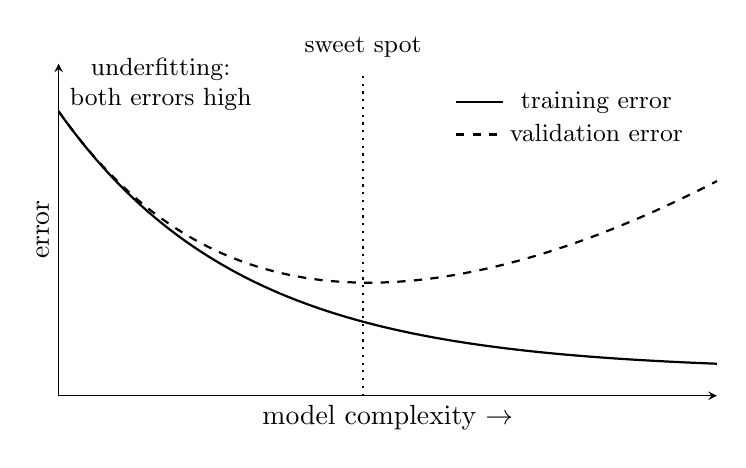
\begin{tikzpicture}
\begin{axis}[
  width=0.82\linewidth, height=5.8cm,
  axis lines=left,
  xlabel={model complexity $\rightarrow$}, ylabel={error},
  ticks=none, domain=0:4, samples=90,
  ymin=0, ymax=1.6, clip=false,
  legend style={draw=none, font=\small, at={(0.97,0.95)}, anchor=north east}
]
\addplot[thick] {1.25*exp(-0.9*x)+0.12};
\addlegendentry{training error}
\addplot[thick, dashed] {1.25*exp(-0.9*x)+0.12+0.055*x^2};
\addlegendentry{validation error}
\draw[dotted, thick] (axis cs:1.85,0) -- (axis cs:1.85,1.55);
\node[font=\small, align=center] at (axis cs:0.62,1.5) {underfitting:\\both errors high};
\node[font=\small, align=center] at (axis cs:3.3,1.32) {overfitting:\\gap grows};
\node[font=\small, align=center] at (axis cs:1.85,1.68) {sweet spot};
\end{axis}
\end{tikzpicture}
\end{utpfig}

\begin{intuition}
For nested model classes with successful optimization, added flexibility cannot worsen the best training fit. Choose capacity using validation, whose error need not follow a smooth U-curve.
\end{intuition}

% === VISUAL ADDITION: three-fit-regimes ===
\subsection{Underfit, good fit, and overfit on the same observations}

The same observations illustrate three levels of flexibility.

\begin{utpfig}[Underfit, good fit, and overfit]{The same observations fitted three ways: a model that is too simple, one that captures the pattern, and one that chases sample noise.}{fig:three-fits}
\begin{tikzpicture}[baseline=(current bounding box.north)]
\begin{axis}[
  width=0.30\linewidth,height=4.0cm,axis lines=left,ticks=none,
  title={Underfit},title style={font=\small\bfseries\color{UTPOrange}},
  xmin=0,xmax=6,ymin=0,ymax=3.2
]
\addplot[only marks,mark=*,mark size=1.6pt,UTPBlue] coordinates
  {(0.5,2.5)(1.3,1.45)(2.1,0.82)(3.0,0.58)(3.8,0.82)(4.7,1.45)(5.5,2.55)};
\addplot[UTPOrange,very thick,domain=0.3:5.7]{1.45};
\node[font=\scriptsize\color{UTPMuted},align=center] at (axis cs:3,2.85) {too simple};
\end{axis}
\end{tikzpicture}
\hfill
\begin{tikzpicture}[baseline=(current bounding box.north)]
\begin{axis}[
  width=0.30\linewidth,height=4.0cm,axis lines=left,ticks=none,
  title={Good fit},title style={font=\small\bfseries\color{UTPGreen}},
  xmin=0,xmax=6,ymin=0,ymax=3.2
]
\addplot[only marks,mark=*,mark size=1.6pt,UTPBlue] coordinates
  {(0.5,2.5)(1.3,1.45)(2.1,0.82)(3.0,0.58)(3.8,0.82)(4.7,1.45)(5.5,2.55)};
\addplot[UTPGreen,very thick,domain=0.3:5.7,samples=80]{0.22*(x-3)^2+0.55};
\node[font=\scriptsize\color{UTPMuted},align=center] at (axis cs:3,2.85) {captures the pattern};
\end{axis}
\end{tikzpicture}
\hfill
\begin{tikzpicture}[baseline=(current bounding box.north)]
\begin{axis}[
  width=0.30\linewidth,height=4.0cm,axis lines=left,ticks=none,
  title={Overfit},title style={font=\small\bfseries\color{UTPRed}},
  xmin=0,xmax=6,ymin=0,ymax=3.2
]
\addplot[only marks,mark=*,mark size=1.6pt,UTPBlue] coordinates
  {(0.5,2.5)(1.3,1.45)(2.1,0.82)(3.0,0.58)(3.8,0.82)(4.7,1.45)(5.5,2.55)};
\addplot[UTPRed,very thick,smooth] coordinates
  {(0.3,2.9)(0.5,2.5)(0.9,0.8)(1.3,1.45)(1.7,2.2)(2.1,0.82)
   (2.55,0.25)(3.0,0.58)(3.35,1.7)(3.8,0.82)(4.25,0.3)(4.7,1.45)
   (5.1,2.95)(5.5,2.55)(5.8,1.1)};
\node[font=\scriptsize\color{UTPMuted},align=center] at (axis cs:3,2.85) {chases sample noise};
\end{axis}
\end{tikzpicture}
\end{utpfig}

\begin{keyidea}
Overfitting means following sample-specific noise, not merely fitting a curve.
\end{keyidea}
% === END VISUAL ADDITION ===

\section{Model capacity and the bias-variance trade-off}\label{sec:bias-variance}

Capacity is representational flexibility. Too little may cause bias; too much may increase sensitivity to sampling noise.

For squared-error regression, the expected error at a point $\bm{x}$ decomposes exactly into three parts. Writing $\hat{f}$ for the model trained on a random dataset and $f$ for the true function with noise variance $\sigma^2$,
\[
  \mathbb{E}\!\left[{(y-\hat{f}(\bm{x}))}^2\right]
  =\underbrace{{\left(\mathbb{E}[\hat{f}(\bm{x})]-f(\bm{x})\right)}^2}_{\text{bias}^2}
  +\underbrace{\operatorname{Var}\!\left(\hat{f}(\bm{x})\right)}_{\text{variance}}
  +\underbrace{\sigma^2}_{\text{irreducible noise}}.
\]
Bias is systematic error; variance is sensitivity to training samples; irreducible noise remains. Regularization trades some bias for lower variance.

\begin{workedexample}
At a fixed test point, let $f(\bm{x})=2$ and $\sigma^2=1$. Compare predictions from three model families, each trained on three random datasets.

\begin{utptable}\small
\begin{tabular}{@{}>{\bfseries\color{UTPNavy}}lcccccc@{}}
\toprule
\rowcolor{UTPPaleBlue!92}
\utpth{Model} & \multicolumn{3}{c}{\bfseries\color{UTPNavy}Predictions} & \utpth{$\text{bias}^2$} & \utpth{Variance} & \utpth{Total} \\
\cmidrule(lr){2-4}
\rowcolor{UTPPaleBlue!92}
 & \utpth{set 1} & \utpth{set 2} & \utpth{set 3} & & & \utpth{($+\,\sigma^2=1$)} \\
\midrule
Rigid    & $2.6$  & $3.0$ & $3.4$ & $1.000$ & $0.107$ & $\mathbf{2.107}$ \\
Balanced & $1.0$  & $2.0$ & $3.0$ & $0.000$ & $0.667$ & $\mathbf{1.667}$ \\
Wild     & $-1.0$ & $2.0$ & $5.0$ & $0.000$ & $6.000$ & $\mathbf{7.000}$ \\
\bottomrule
\end{tabular}
\end{utptable}

The first row averages $3.0$ against truth $2$, giving bias $1$ and squared bias $1$. Its variance is
\[
  \frac{{(2.6-3)}^2+{(3.0-3)}^2+{(3.4-3)}^2}{3}=\frac{0.16+0+0.16}{3}\approx 0.107,
\]
and the total is $1.000+0.107+1=2.107$.

The rigid model is biased; the wild model is unbiased but highly variable. Minimize total error, not bias alone.

Every row includes irreducible noise $\sigma^2=1$, so no model can reduce expected error below~$1$.
\end{workedexample}

\begin{intuition}
Bias is a tight group of darts away from the bullseye; variance is a wide scatter around it. Irreducible noise is a wobbling dartboard.
\end{intuition}

More data often reduces variance; stronger assumptions may exchange bias for lower variance. Choose reliable validation performance over complexity.

\section{Regularization}

Regularization discourages unnecessarily large or complex parameter values. Two common penalties are
\[
  J_{L_1}(\bm{\theta})=J(\bm{\theta})
  +\lambda\sum_{j=1}^{p}|\theta_j|,
\]
\[
  J_{L_2}(\bm{\theta})=J(\bm{\theta})
  +\lambda\sum_{j=1}^{p}\theta_j^2.
\]
$L_1$ regularization can make some parameters exactly zero. $L_2$ regularization smoothly shrinks large parameters. The strength $\lambda$ is normally selected with validation data.

\begin{workedexample}
For the one-parameter objective $\tfrac12(\beta-\hat\beta_{\text{OLS}})^2$ with $\hat\beta_{\text{OLS}}=4$, ridge adds $\lambda\beta^2/2$ and lasso adds $\lambda|\beta|$. Their solutions are
\[
  \hat{\beta}_{\text{ridge}}=\frac{\hat{\beta}_{\text{OLS}}}{1+\lambda},
  \qquad
  \hat{\beta}_{\text{lasso}}=\operatorname{sign}(\hat{\beta}_{\text{OLS}})\max\!\left(|\hat{\beta}_{\text{OLS}}|-\lambda,\;0\right).
\]

\begin{utptable}\small
\begin{tabular}{@{}cccl@{}}
\toprule
\rowcolor{UTPPaleBlue!92}
\utpth{$\lambda$} & \utpth{Ridge} & \utpth{Lasso} & \utpth{What happened} \\
\midrule
$0$ & $4.000$ & $4.000$ & no penalty; both give the OLS answer \\
$1$ & $2.000$ & $3.000$ & ridge halves it; lasso subtracts a flat $1$ \\
$5$ & $0.667$ & $0.000$ & ridge is small but alive; lasso has deleted the feature \\
\bottomrule
\end{tabular}
\end{utptable}

Here ridge divides by $1+\lambda$, approaching zero without reaching it at finite $\lambda$. Lasso subtracts $\lambda$ and clips at zero once $\lambda\ge4$.
\end{workedexample}

\subsection{Other ways to regularize}

Regularization is broader than adding a penalty to the objective.

\begin{itemize}
  \item \term{Early stopping} retains the model from the epoch with the best validation performance.
  \item \term{Data augmentation} adds meaningful input variation without changing labels.
    \item \term{Pruning} removes weak branches, features, or parameters.
  \item \term{Ensembling} averages several models to reduce variance.
  \item \term{Noise injection} trains the model to remain stable under small perturbations.
\end{itemize}

Match regularization to the failure mode; it cannot fix leakage or distribution mismatch.

\section{Learning curves}

A learning curve plots training and validation performance against training-set size or training time.

\begin{itemize}
  \item Poor training and validation performance suggests underfitting or an optimization problem.
  \item Strong training performance with weak validation performance suggests overfitting.
  \item Improvement in both curves as more data is added suggests that additional representative data may help.
  \item Highly unstable curves suggest sensitivity to the split, seed, or a small validation sample.
\end{itemize}

\subsection{Reading learning curves in practice}

\begin{utpfig}[Reading learning curves]{Learning curves: training and validation error against training-set size. A persistent gap between the curves suggests variance; two curves that are both poor suggest limited signal or underfitting.}{fig:learning-curves}
\begin{tikzpicture}[baseline=(current bounding box.north)]
\begin{axis}[
  width=0.46\linewidth, height=4.3cm, axis lines=left,
  title style={font=\small\bfseries\color{UTPRed}}, title={High variance (overfitting)},
  xlabel={Training rows}, ylabel={Error},
  label style={font=\scriptsize\color{UTPMuted}}, tick label style={font=\scriptsize\color{UTPMuted}},
  legend style={font=\scriptsize,draw=none,fill=none,at={(0.98,0.96)},anchor=north east},
  xmin=0, xmax=1000, ymin=0, ymax=0.5
]
\addplot[UTPBlue,very thick,mark=*,mark size=1.2pt] coordinates
  {(50,0.01)(150,0.02)(300,0.03)(600,0.04)(1000,0.05)}; \addlegendentry{train}
\addplot[UTPRed,very thick,mark=square*,mark size=1.2pt] coordinates
  {(50,0.45)(150,0.36)(300,0.31)(600,0.27)(1000,0.25)}; \addlegendentry{validation}
\end{axis}
\end{tikzpicture}
\hfill
\begin{tikzpicture}[baseline=(current bounding box.north)]
\begin{axis}[
  width=0.46\linewidth, height=4.3cm, axis lines=left,
  title style={font=\small\bfseries\color{UTPOrange}}, title={High bias (underfitting)},
  xlabel={Training rows}, ylabel={Error},
  label style={font=\scriptsize\color{UTPMuted}}, tick label style={font=\scriptsize\color{UTPMuted}},
  legend style={font=\scriptsize,draw=none,fill=none,at={(0.98,0.96)},anchor=north east},
  xmin=0, xmax=1000, ymin=0, ymax=0.5
]
\addplot[UTPBlue,very thick,mark=*,mark size=1.2pt] coordinates
  {(50,0.20)(150,0.24)(300,0.26)(600,0.27)(1000,0.28)}; \addlegendentry{train}
\addplot[UTPRed,very thick,mark=square*,mark size=1.2pt] coordinates
  {(50,0.38)(150,0.33)(300,0.31)(600,0.30)(1000,0.30)}; \addlegendentry{validation}
\end{axis}
\end{tikzpicture}
\end{utpfig}

\begin{keyidea}
A persistent gap suggests variance: try more representative data or stronger regularization. Both curves poor suggest limited signal, underfitting, or optimization failure; investigate features and fitting.
\end{keyidea}

\section{Hyperparameter tuning}
\label{sec:hyperparameter-tuning}

Hyperparameters include regularization strength, tree depth, number of neighbors, learning rate, and model size. Common search methods are:

\begin{utptable}
\begin{tabularx}{\linewidth}{@{}>{\bfseries\leavevmode\color{UTPNavy}}m{0.22\linewidth}m{0.39\linewidth}X@{}}
\toprule
\rowcolor{UTPPaleBlue!92}
\utpth{Method} & \utpth{Search strategy} & \utpth{Main consideration} \\
\midrule
Grid search & Evaluates every combination in a fixed Cartesian grid. & Becomes expensive as the number of dimensions and candidate values grows. \\
Random search & Samples combinations from the search space. & Often explores high-dimensional spaces more efficiently. \\
Sequential search & Uses earlier results to choose promising later experiments. & Concentrates the search on regions that appear useful. \\
\bottomrule
\end{tabularx}
\end{utptable}

Use identical validation across candidates. Repeated tuning can overfit validation, so retain an untouched final test set.

\subsection{Tuning without fooling yourself}

\begin{intuition}
Random search explores more distinct values when few hyperparameters matter. Small grids suit one or two controls; neither fixes invalid validation.
\end{intuition}

\subsection{Nested cross-validation for the selection procedure}

Tune inside each outer training split; outer holdouts evaluate the complete search-plus-model procedure. Lab~2, Part~D instead uses one training-only search and a final test.

\section{Imbalanced classification: change the policy, not the test set}

Imbalance can make majority predictions look accurate while missing rare cases. Consider metrics, thresholds, class weights, and training-only resampling.

\begin{utptable}
\begin{tabularx}{\linewidth}{@{}>{\bfseries\leavevmode\color{UTPNavy}}m{0.24\linewidth}X@{}}
\toprule
\rowcolor{UTPPaleBlue!92}
\utpth{Strategy} & \utpth{How it helps} \\
\midrule
Change the metric first & For rare-class performance, use recall, precision, balanced accuracy, or average precision rather than accuracy alone (\chapref{ch:evaluation}). \\
Move the threshold & Choose a lower probability cutoff on validation data to increase recall without retraining. \\
Class weights & Tell the model that a mistake on the rare class costs more (\texttt{class\_weight="balanced"}). Lab~2's grid search includes this option and selects it. \\
Resampling & Drop majority rows (\term{undersampling}) or add minority examples (\term{oversampling}). SMOTE interpolates between nearby minority examples. Resample only within each validation split\textquotesingle s training portion. \\
\bottomrule
\end{tabularx}
\end{utptable}

\begin{coursechoice}
SMOTE's geometry is developed in \chapref{ch:knn-nb}. Its rule applies now: split first and synthesize only within training folds, never from held-out observations.
\end{coursechoice}

\begin{pitfall}
Resampling changes training prevalence, not the target evaluation population. Keep validation and test distributions realistic.
\end{pitfall}

\section{Feature selection is part of model development} \label{sec:feature-selection}

\term{Feature selection} keeps a subset of the original columns to cut cost, noise, or complexity. It is not always worth doing: a regularized model with a modest number of features may not need it.

Selection retains original columns; extraction creates new ones, as in PCA (\chapref{ch:dimred}).

\begin{utptable}
\begin{tabularx}{\linewidth}{@{}>{\bfseries\leavevmode\color{UTPNavy}}m{0.19\linewidth}m{0.38\linewidth}X@{}}
\toprule
\rowcolor{UTPPaleBlue!92}
\utpth{Family} & \utpth{How it works} & \utpth{Main trade-off} \\
\midrule
Filter methods & Score features by variance, correlation, tests, or mutual information before model fitting. & Fast and model-agnostic, but may miss interactions. \\
Wrapper methods & Fit a model on different feature subsets, as in recursive feature elimination. & Model-specific, but computationally expensive. \\
Embedded methods & Use selection learned during fitting: zero lasso coefficients or tree-based importances. & Efficient, but inherits model assumptions and instability. \\
\bottomrule
\end{tabularx}
\end{utptable}

\begin{secondpass}
Revisit lasso in \chapref{ch:regression}, tree importances in \chapsref{ch:decision-trees}{ch:ensembles}, and irrelevant dimensions in \chapref{ch:knn-nb}. The validation rules stay the same.
\end{secondpass}

\begin{pitfall}
Fit supervised selectors inside the validated pipeline, separately in each training fold. Selecting once on all labels leaks information; the number of retained features is also a hyperparameter.
\end{pitfall}

\begin{keyidea}
Before selecting features, specify the goal: accuracy, collection cost, or interpretability. Validate selection together with the model, without using the test set.
\end{keyidea}

\begin{debugtask}
A researcher selects the top 20 features using all labeled rows, applies SMOTE to the full table, then runs cross-validation and reports the best result. Redesign the experiment so that nothing from the held-out rows can influence selection, resampling, or tuning.
\end{debugtask}

\section{Reproducible training}

A reproducible experiment records:

\begin{itemize}
  \item data and preprocessing versions;
  \item training, validation, and test identifiers;
  \item software and hardware environment;
  \item model specification and configuration;
  \item hyperparameters, random seeds, and stopping rules;
  \item training curves, checkpoints, and evaluation outputs.
\end{itemize}

Report variation across reruns rather than one favorable seed; parallel hardware may prevent bit-for-bit reproduction.

\begin{keyidea}
Training fit and generalization are distinct requirements.
\end{keyidea}

\begin{modelcard}{Training and Tuning - Practical Checklist}
\begin{tabularx}{\linewidth}{@{}>{\bfseries\leavevmode\color{UTPNavy}}p{0.24\linewidth}X@{}}
Objective & Define the training objective and know which parts are learned from data; optimizer details are second-pass when the estimator exposes them. \cr
Diagnosis & Compare training and validation curves to identify underfitting or overfitting. \cr
Regularization & Limit model capacity with penalties, pruning, simpler features, or early stopping. \cr
Tuning & Search hyperparameters using validation data or nested cross-validation, not the final test set. \cr
Reproducibility & Record the data version, split logic, preprocessing, model specification, random seeds, software versions, and hardware-relevant settings. \cr
\end{tabularx}
\end{modelcard}

\subsection{A short reproducibility checklist}

\begin{utptable}
\begin{tabularx}{\linewidth}{@{}>{\bfseries\leavevmode\color{UTPNavy}}m{0.05\linewidth}X@{}}
\toprule
\rowcolor{UTPPaleBlue!92}
\utpth{\checkmark} & \utpth{Record this before you call a model finished} \\
\midrule
1 & The exact data snapshot, with a date and a row count. \\
2 & Every random seed used. \\
3 & Library versions. \\
4 & The complete preprocessing and modeling procedure, not only the final estimator. \\
5 & The chosen hyperparameters and the search space they came from. \\
6 & The metric, the split strategy, and the final test score. \\
7 & Known limitations: who the model is likely to be wrong about. \\
\bottomrule
\end{tabularx}
\end{utptable}

\begin{keyidea}
Record weakly represented populations and known subgroup failures. These limits guide responsible use, not a judgment that the project failed.
\end{keyidea}

\subsection{Save the model you would deploy}

After locking and testing the procedure, save the whole preprocessing-and-estimator pipeline with a model card for reuse.

\begin{lstlisting}[style=utppython]
import joblib, json

joblib.dump(final_model, MODELS / "titanic_survival.joblib")
(MODELS / "titanic_survival_card.json").write_text(json.dumps({
    "features": features,                 # the columns the model expects
    "final_test_roc_auc": 0.837,          # the one test result
    "decision_threshold": 0.5,            # the policy chosen on validation data
    "scikit_learn_version": sklearn.__version__,
}, indent=2))

loaded = joblib.load(MODELS / "titanic_survival.joblib")
loaded.predict_proba(new_rows)            # new_rows has the same columns as training
\end{lstlisting}

Verify the saved artifact:

\begin{itemize}
  \item \textbf{Save the pipeline.} Include fitted scaling and encoding, not just the estimator.
  \item \textbf{Check that the file reproduces the test predictions.} Load it back and compare with the in-memory model before calling it done.
  \item \textbf{Include a model card:} features, threshold, test score, and library version. Lab~2 saves the model; Lab~3 verifies it; \texttt{predict\_passenger.py} loads it.
\end{itemize}

\begin{tryit}
Repeat training and validation across prespecified seeds and splits. Report variation, lock the seed policy and model, refit, then test once.
\end{tryit}

\begin{debugtask}
A hyperparameter search reports its best configuration, then the researcher reruns the search with a narrower grid chosen after inspecting the test score. Explain how the test set entered training decisions and redesign the selection/final-evaluation boundary.
\end{debugtask}

\begin{decisionmemo}
Two models have nearly equal mean validation performance. One has lower fold-to-fold variation, half the inference latency, and simpler monitoring. Decide which to keep and state why a tiny mean-score advantage is not automatically decisive.
\end{decisionmemo}

\begin{tryit}
Using fixed validation folds, compare training and validation performance across capacities. Tune on development data, lock the procedure, and list the refitting steps before one final test.
\end{tryit}

\begin{quickcheck}
\begin{enumerate}
  \item What train-versus-validation pattern suggests underfitting, and what pattern suggests overfitting?
  \item How can regularization improve validation performance even while making the training fit worse?
  \item Which decisions must be locked before the final test set is evaluated?
\end{enumerate}
\end{quickcheck}

\substage{3B}{Supervised Model Families}{Compare model families under one fixed validation workflow.}
\chapter{Linear Models for Regression}
\label{ch:regression}

\chapterguide%
  {\chapref{ch:supervised}, \chapref{ch:training}, and vectors/matrices from \chapref{ch:linear-algebra}.}
  {fit and interpret linear regression, diagnose residuals, engineer nonlinear terms, and regularize coefficients.}

Linear regression makes capacity, regularization, and optimization explicit. Through \chapref{ch:svm}, compare model families under the same workflow.

\section{The model}

Linear regression predicts a continuous value using a weighted sum of features:
\[
  \hat{y}=\beta_0+\beta_1x_1+\cdots+\beta_{p}x_{p}.
\]
$\beta_0$ predicts at zero-valued features; $\beta_j$ is the prediction change per unit of $x_j$, holding other features fixed.

\section{Least squares: how the line is chosen}

Ordinary least squares (OLS) chooses coefficients that minimize the residual sum of squares:
\[
  \min_{\bm{\beta}}
  \sum_{i=1}^{n}{(y_i-\hat{y}_i)}^2.
\]
A \term{residual}, $y_i-\hat y_i$, is the observed minus predicted value.

\begin{utpfig}[Least squares]{Least squares chooses the line that minimizes the sum of squared vertical distances between the observations and the line.}{fig:least-squares}
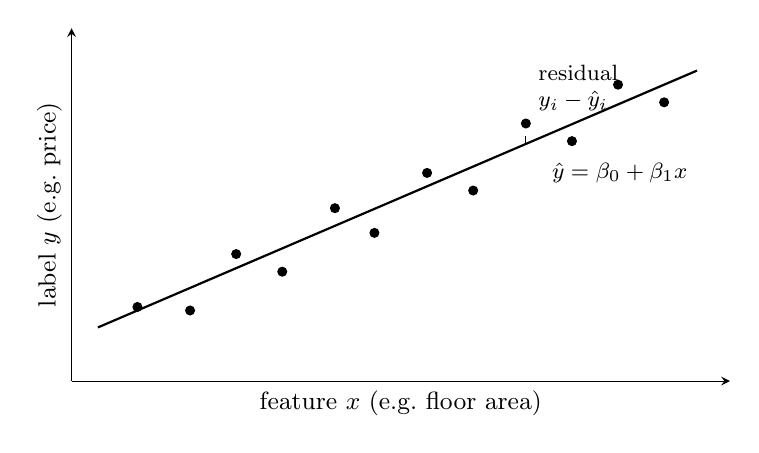
\begin{tikzpicture}
\begin{axis}[
  width=0.82\linewidth, height=0.50\linewidth,
  axis lines=left,
  xlabel={feature $x$ (e.g.\ floor area)},
  ylabel={label $y$ (e.g.\ price)},
  label style={font=\small},
  ticks=none, xmin=0, xmax=10, ymin=0, ymax=10,
  clip=false
]
\addplot[only marks, mark=*, mark size=1.6pt] coordinates {
  (1,2.1) (1.8,2.0) (2.5,3.6) (3.2,3.1) (4.0,4.9)
  (4.6,4.2) (5.4,5.9) (6.1,5.4) (6.9,7.3) (7.6,6.8)
  (8.3,8.4) (9.0,7.9)
};
\addplot[thick, domain=0.4:9.5] {0.8*x + 1.2};
\draw[dashed] (axis cs:6.9,6.72) -- (axis cs:6.9,7.3)
  node[above right=1pt, font=\footnotesize, align=left]
    {residual\\$y_i-\hat{y}_i$};
\node[font=\footnotesize, anchor=east]
  at (axis cs:9.5,5.9) {$\hat{y}=\beta_0+\beta_1 x$};
\end{axis}
\end{tikzpicture}
\end{utpfig}

\begin{intuition}
Imagine rubber bands pulling observations toward the line. Least squares minimizes their total squared vertical lengths.
\end{intuition}

With a single feature, the best-fitting slope and intercept have simple closed forms:
\[
  \hat{\beta}_1
  =\frac{\sum_{i=1}^{n}(x_i-\bar{x})(y_i-\bar{y})}
        {\sum_{i=1}^{n}{(x_i-\bar{x})}^2},
  \qquad
  \hat{\beta}_0=\bar{y}-\hat{\beta}_1\bar{x}.
\]
Slope is covariance divided by feature variance. The intercept makes the line pass through $(\bar x,\bar y)$.

\begin{workedexample}
Fit a line to three points by hand: $(1,2)$, $(2,3)$, $(3,5)$.
The means are $\bar{x}=2$ and $\bar{y}=10/3$. The deviations from the means are $(-1,0,1)$ for $x$ and $(-\tfrac{4}{3},-\tfrac{1}{3},\tfrac{5}{3})$ for $y$. Then
\[
  \hat{\beta}_1
  =\frac{(-1)(-\tfrac{4}{3})+(0)(-\tfrac{1}{3})+(1)(\tfrac{5}{3})}
        {{(-1)}^2+0^2+1^2}
  =\frac{3}{2}=1.5,
  \qquad
  \hat{\beta}_0=\tfrac{10}{3}-1.5\times 2=\tfrac{1}{3}\approx 0.33.
\]
The fitted line is $\hat{y}=0.33+1.5x$, giving predictions $1.83$, $3.33$, and $4.83$ with residuals $+0.17$, $-0.33$, and $+0.17$. The residuals sum to zero --- a general property of least squares with an intercept.
\end{workedexample}

\section{Many features: the matrix view}

With the intercept absorbed into a leading column of ones in the design matrix $X\in\mathbb{R}^{n\times(p+1)}$, the objective and its gradient are
\[
  J(\bm{\beta})=\frac{1}{n}\|X\bm{\beta}-\bm{y}\|_2^2,
  \qquad
  \nabla_{\bm{\beta}}J
  =\frac{2}{n}X^{\mathsf T}(X\bm{\beta}-\bm{y}).
\]
Setting the gradient to zero gives the \term{normal equations} $X^{\mathsf T}X\bm{\beta}=X^{\mathsf T}\bm{y}$, whose solution (when $X^{\mathsf T}X$ is invertible) is
\[
  \hat{\bm{\beta}}={(X^{\mathsf T}X)}^{-1}X^{\mathsf T}\bm{y}.
\]
Solve the linear system with a stable factorization, or use gradient descent for large datasets. Explicit inversion is a teaching device, not the usual numerical approach.

\subsection{Reading the coefficients honestly}

\begin{itemize}
  \item Coefficients are in the label's units per unit of the feature, so their sizes are not comparable unless the features are standardized first.
  \item \term{Multicollinearity}: correlated features make individual coefficients unstable, even when predictions remain accurate.
  \item Coefficients are associations, not causal effects (\secref{sec:correlation}); adding or removing one feature can change the sign of another coefficient.
\end{itemize}

\subsection{The assumptions, in plain words}

Classical OLS assumptions include linearity in the chosen features, independent errors, constant error variance, and no exact collinearity. Violations can undermine coefficient interpretation and uncertainty estimates; inspect residuals for warning signs.

\section{Reading residuals: the diagnostic that matters most}

Inspect residuals $y-\hat y$ for structure the fitted model missed.

\begin{utpfig}[Reading residuals]{Two residual plots. A healthy fit leaves a formless cloud around zero; an obvious curve is structure the model has missed.}{fig:residuals}
\begin{tikzpicture}[baseline=(current bounding box.north)]
\begin{axis}[
  width=0.46\linewidth, height=4.1cm, axis lines=left,
  title style={font=\small\bfseries\color{UTPGreen}}, title={Healthy: a formless cloud},
  xlabel={Prediction $\hat y$}, ylabel={Residual},
  label style={font=\scriptsize\color{UTPMuted}}, tick label style={font=\scriptsize\color{UTPMuted}},
  xmin=0, xmax=10, ymin=-3, ymax=3
]
\addplot[only marks,mark=*,mark size=1.2pt,UTPGreen] coordinates {
(0.6,0.7)(1.2,-0.9)(1.8,0.3)(2.4,-1.4)(3.0,1.1)(3.6,-0.4)(4.2,1.6)(4.8,-1.1)
(5.4,0.2)(6.0,-1.7)(6.6,1.3)(7.2,-0.6)(7.8,0.9)(8.4,-1.2)(9.0,0.5)(9.5,-0.3)};
\draw[UTPNavy,thick,dashed] (axis cs:0,0) -- (axis cs:10,0);
\end{axis}
\end{tikzpicture}
\hfill
\begin{tikzpicture}[baseline=(current bounding box.north)]
\begin{axis}[
  width=0.46\linewidth, height=4.1cm, axis lines=left,
  title style={font=\small\bfseries\color{UTPRed}}, title={Sick: an obvious curve},
  xlabel={Prediction $\hat y$}, ylabel={Residual},
  label style={font=\scriptsize\color{UTPMuted}}, tick label style={font=\scriptsize\color{UTPMuted}},
  xmin=0, xmax=10, ymin=-3, ymax=3
]
\addplot[only marks,mark=*,mark size=1.2pt,UTPRed] coordinates {
(0.6,2.1)(1.2,1.4)(1.8,0.6)(2.4,0.1)(3.0,-0.6)(3.6,-1.2)(4.2,-1.6)(4.8,-1.9)
(5.4,-1.8)(6.0,-1.5)(6.6,-1.0)(7.2,-0.3)(7.8,0.5)(8.4,1.3)(9.0,2.0)(9.5,2.5)};
\draw[UTPNavy,thick,dashed] (axis cs:0,0) -- (axis cs:10,0);
\end{axis}
\end{tikzpicture}
\end{utpfig}

\begin{keyidea}
Residual patterns suggest missing structure: curvature suggests nonlinear terms; a widening funnel suggests unequal error variance. Lab~2's insurance bands motivate a smoker $\times$ BMI interaction.
\end{keyidea}

\section{Polynomial regression: curves from a linear model}

Linear models are linear \emph{in parameters}. Adding $x^2$, $x^3$, or $x_1x_2$ allows curved predictions:
\[
  \hat{y}=\beta_0+\beta_1x+\beta_2x^2+\cdots+\beta_dx^d.
\]
Polynomial degree $d$ controls capacity; excessive degree can fit noise.

\begin{utpfig}[Polynomial degree]{Polynomial degree controls capacity. A straight line underfits a curved pattern, a quadratic captures it, and a high-degree fit starts to follow the noise.}{fig:poly-degree}
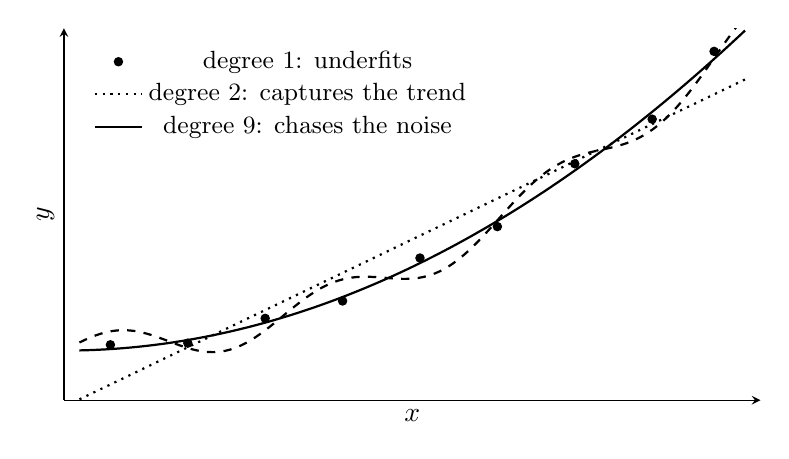
\begin{tikzpicture}
\begin{axis}[
  width=0.86\linewidth, height=0.52\linewidth,
  axis lines=left,
  xlabel={$x$}, ylabel={$y$},
  ticks=none, xmin=0, xmax=4.5, ymin=-3, ymax=19.5,
  legend style={draw=none, font=\small, at={(0.03,0.97)}, anchor=north west},
  clip=true
]
\addplot[only marks, mark=*, mark size=1.5pt] coordinates {
  (0.3,0.35) (0.8,0.45) (1.3,1.95) (1.8,3.0) (2.3,5.6)
  (2.8,7.5) (3.3,11.3) (3.8,14.0) (4.2,18.1)
};
\addplot[thick, dotted, domain=0.1:4.4, samples=60] {4.5*x-3.4};
\addlegendentry{degree 1: underfits}
\addplot[thick, domain=0.1:4.4, samples=80] {x^2};
\addlegendentry{degree 2: captures the trend}
\addplot[thick, dashed, domain=0.1:4.4, samples=160] {x^2 + 1.1*sin(deg(4.5*x))};
\addlegendentry{degree 9: chases the noise}
\end{axis}
\end{tikzpicture}
\end{utpfig}

\begin{intuition}
Low degree may underfit; high degree may interpolate noise. Select degree using validation, not training fit.
\end{intuition}

Polynomial feature counts grow quickly, motivating regularization.

\section{Ridge regression: shrink everything a little}

\term{Ridge regression} adds an $L_2$ penalty on coefficient size to the least-squares objective. For centered features and label (so the intercept has been removed), its solution is
\[
  \hat{\bm{\beta}}_{\mathrm{ridge}}
  =\argmin_{\bm{\beta}}
  \|X\bm{\beta}-\bm{y}\|_2^2
  +\lambda\|\bm{\beta}\|_2^2
  ={(X^{\mathsf T}X+\lambda I)}^{-1}X^{\mathsf T}\bm{y}.
\]
The penalty trades fit against coefficient size. At $\lambda=0$, ridge is OLS; increasing $\lambda$ shrinks penalized coefficients. For $\lambda>0$, the centered system is invertible. Software usually leaves the intercept unpenalized and recovers it from the means.

\section{Lasso: shrink some coefficients to exactly zero}

\term{Lasso regression} swaps the penalty for an $L_1$ norm:
\[
  \hat{\bm{\beta}}_{\mathrm{lasso}}
  =\argmin_{\bm{\beta}}
  \|X\bm{\beta}-\bm{y}\|_2^2
  +\lambda\|\bm{\beta}\|_1.
\]
Lasso sets some coefficients exactly to zero, producing sparse models. Among strongly correlated features, however, it may choose one somewhat arbitrarily.

\subsection{Why the penalties behave differently}

Regularization constrains a coefficient budget. Least-squares contours touch an $L_1$ diamond often at axis corners, where coefficients are zero; an $L_2$ disk has no such corners.

\begin{utpfig}[Why lasso zeroes coefficients]{Why the penalties behave differently. The least-squares contours often first touch the $L_1$ diamond at a corner, where a coefficient is exactly zero; the $L_2$ disk has no corners, so ridge shrinks both coefficients without zeroing either.}{fig:lasso-ridge}
\begin{tikzpicture}[x=0.92cm, y=0.92cm, font=\small]
% ---- lasso panel ----
\begin{scope}
\draw[-{Stealth[length=2mm]}] (-1.5,0) -- (3.6,0) node[below] {$\beta_1$};
\draw[-{Stealth[length=2mm]}] (0,-1.1) -- (0,2.2);
\node[left] at (0,1.9) {$\beta_2$};
\draw[thick, fill=gray!18] (1,0) -- (0,1) -- (-1,0) -- (0,-1) -- cycle;
\draw[rotate around={39:(2.1,0.9)}] (2.1,0.9) ellipse (0.52 and 0.25);
\draw[rotate around={39:(2.1,0.9)}] (2.1,0.9) ellipse (0.95 and 0.45);
\draw[rotate around={39:(2.1,0.9)}] (2.1,0.9) ellipse (1.42 and 0.67);
\fill (2.1,0.9) circle (1.6pt) node[above right=0pt] {OLS fit};
\fill (1,0) circle (2pt);
\node[anchor=north, align=center, font=\footnotesize]
  at (1,-1.22) {lasso fit: $\beta_2=0$};
\node[anchor=west] at (0.35,2.65) {$L_1$ budget (diamond)};
\end{scope}
% ---- ridge panel ----
\begin{scope}[xshift=6.0cm]
\draw[-{Stealth[length=2mm]}] (-1.5,0) -- (3.6,0) node[below] {$\beta_1$};
\draw[-{Stealth[length=2mm]}] (0,-1.1) -- (0,2.2);
\node[left] at (0,1.9) {$\beta_2$};
\draw[thick, fill=gray!18] (0,0) circle (1);
\draw[rotate around={39:(2.1,0.9)}] (2.1,0.9) ellipse (0.52 and 0.25);
\draw[rotate around={39:(2.1,0.9)}] (2.1,0.9) ellipse (0.95 and 0.45);
\draw[rotate around={39:(2.1,0.9)}] (2.1,0.9) ellipse (1.35 and 0.64);
\fill (2.1,0.9) circle (1.6pt) node[above right=0pt] {OLS fit};
\fill (0.98,0.19) circle (2pt);
\node[anchor=north, align=center, font=\footnotesize]
  at (1,-1.22) {ridge fit: both small, neither zero};
\node[anchor=west] at (0.35,2.65) {$L_2$ budget (disk)};
\end{scope}
\end{tikzpicture}
\end{utpfig}

\begin{intuition}
Regularization pulls coefficients toward zero: ridge shrinks them smoothly, while lasso can remove them entirely.
\end{intuition}

\section{Elastic net and practical guidance}

\term{Elastic net} combines both penalties,
\[
  \lambda\!\left(
  \rho\,\|\bm{\beta}\|_1
  +(1-\rho)\,\|\bm{\beta}\|_2^2
  \right),
\]
gaining lasso's sparsity while sharing weight across correlated features like ridge. The mixing parameter $\rho$ and strength $\lambda$ are both tuned on validation data.

Working habits that apply to every model in this chapter:

\begin{itemize}
  \item \term{Standardize features} so penalties act on comparable scales. Usually leave the intercept unpenalized.
  \item \term{Tune $\lambda$ with cross-validation} (\chapref{ch:evaluation}), searching over a logarithmic grid such as $10^{-3}$, $10^{-2}$, \ldots, $10^{2}$.
  \item \term{Starting choices:} ridge for many small effects; lasso for sparsity; elastic net for correlated groups.
  \item Consider \term{Huber loss} when extreme residuals dominate squared-error fitting.
\end{itemize}

\begin{keyidea}
A weighted-sum model, richer features, and a validated complexity penalty form a reusable modeling pattern.
\end{keyidea}

\begin{modelcard}{Linear Regression Family - Quick Guide}
\begin{tabularx}{\linewidth}{@{}>{\bfseries\leavevmode\color{UTPNavy}}p{0.24\linewidth}X@{}}
Best when & The label is numerical, a weighted-sum relationship is a useful approximation, and interpretability matters. \cr
Start with & Ordinary linear regression, residual plots, and a mean/median baseline. \cr
Preprocessing & Encode categories; standardize before ridge, lasso, or elastic net; inspect skew and outliers. \cr
Main controls & Polynomial degree, regularization strength $\lambda$, and elastic-net mixing parameter. \cr
Watch for & Nonlinearity, influential outliers, multicollinearity, leakage, and unsafe extrapolation beyond the training range. \cr
\end{tabularx}
\end{modelcard}

\section{When ordinary squared error is the wrong model for the label}
\label{sec:special-regression-labels}

Use a different loss or distribution when the label structure or decision warrants it, not merely to make the model more elaborate.

\begin{utptable}
\begin{tabularx}{\linewidth}{@{}m{0.22\linewidth}m{0.29\linewidth}X@{}}
\toprule
\rowcolor{UTPPaleBlue!92}
\utpth{Label structure} & \utpth{Useful starting point} & \utpth{Main caution} \\
\midrule
Continuous values with occasional large errors & Robust regression loss & Robustness changes which errors receive the most influence; validate against the real evaluation objective. \\
Conditional quantiles matter & Quantile regression & Different quantiles answer different questions and should not be interpreted as conditional means. \\
Non-negative counts & Count-aware generalized linear model & The chosen distributional assumptions must be plausible for the observed mean--variance relationship. \\
Positively skewed outcomes & Log-scale modeling or an appropriate positive-response model & Back-transformation changes the interpretation of average predictions and errors. \\
\bottomrule
\end{tabularx}
\end{utptable}

Validate specialized losses against the task metric and check prediction plausibility (\chapref{ch:evaluation}).

\begin{quickcheck}
\begin{enumerate}
  \item What does a regression coefficient mean when the other modeled features are held fixed, and why is that not automatically a causal effect?
  \item How do ridge and lasso change coefficient estimates differently as regularization becomes stronger?
  \item How can an interaction or polynomial feature let a model remain linear in its parameters while representing a nonlinear relationship in the original inputs?
\end{enumerate}
\end{quickcheck}
\chapter{Linear Models for Classification}
\label{ch:classification}

\chapterguide%
  {\chapref{ch:supervised}, \chapref{ch:training}, and probability/odds from \chapref{ch:statistics}.}
  {interpret logistic, softmax, ordinal, and discriminant models; tune thresholds and compare linear classifiers.}

Linear classifiers separate categories with flat boundaries. Logistic regression, discriminant analysis, and the perceptron choose those boundaries differently; QDA extends discriminant analysis to curved boundaries.

\section{Why not just use linear regression?}

OLS on $0/1$ labels can predict outside $[0,1]$. Logistic regression constrains probabilities and fits them with cross-entropy.

\section{From probabilities to odds to a linear model}

\term{Odds} are $p/(1-p)$: $p=0.75$ gives odds~3. Their logarithm, the \term{logit}, spans the real line. Logistic regression assumes linear log-odds:

\begin{utptable}
\begin{tabularx}{0.78\linewidth}{@{}>{\bfseries\leavevmode\color{UTPNavy}}X X X@{}}
\toprule
\rowcolor{UTPPaleBlue!92}
\utpth{Probability} & \utpth{Odds} & \utpth{Read aloud} \\
\midrule
$50\%$ & $1:1$ & equally likely either way \\
$75\%$ & $3:1$ & three chances for, one against \\
$90\%$ & $9:1$ & nine chances for, one against \\
\bottomrule
\end{tabularx}
\end{utptable}

\[
  \log\frac{p}{1-p}
  =\beta_0+\bm{\beta}^{\mathsf T}\bm{x}.
\]
Solving for $p$ inverts the logarithm and produces the familiar S-shaped \term{sigmoid}:
\[
  P(Y=1\given\bm{x})
  =\sigma(z)
  =\frac{1}{1+e^{-z}},
  \qquad
  z=\beta_0+\bm{\beta}^{\mathsf T}\bm{x}.
\]

\begin{utpfig}[The sigmoid]{The sigmoid maps an unrestricted score to a probability. Scores near zero give probabilities near $0.5$; large positive or negative scores give confident answers.}{fig:sigmoid}
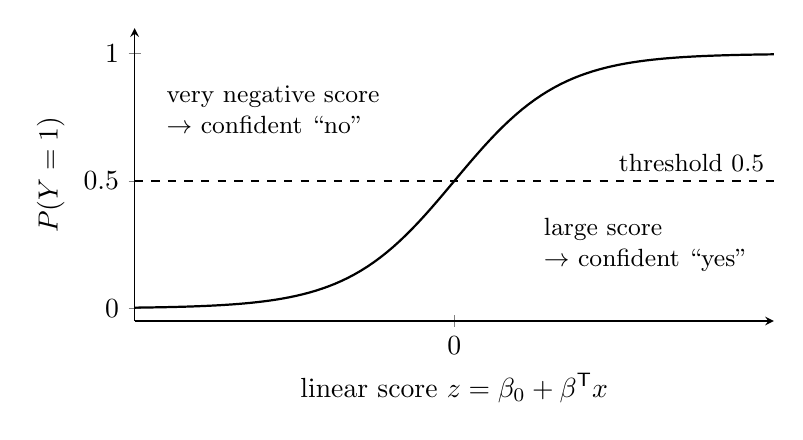
\begin{tikzpicture}
\begin{axis}[
  width=0.80\linewidth, height=5.3cm,
  axis lines=left,
  xlabel={linear score $z=\beta_0+\bm{\beta}^{\mathsf T}\bm{x}$},
  ylabel={$P(Y=1)$},
  ytick={0,0.5,1}, xtick={0},
  domain=-6:6, samples=100, ymin=-0.05, ymax=1.1, clip=false
]
\addplot[thick] {1/(1+exp(-x))};
\draw[dashed] (axis cs:-6,0.5) -- (axis cs:6,0.5)
  node[above left, font=\small] {threshold $0.5$};
\node[font=\small, align=left] at (axis cs:3.6,0.25) {large score\\$\rightarrow$ confident ``yes''};
\node[font=\small, align=left] at (axis cs:-3.4,0.78) {very negative score\\$\rightarrow$ confident ``no''};
\end{axis}
\end{tikzpicture}
\end{utpfig}

\begin{intuition}
The sigmoid maps an unrestricted score to a probability. Scores near zero give probabilities near $0.5$; large magnitudes indicate confidence.
\end{intuition}

A unit increase in $x_j$ multiplies the odds by $e^{\beta_j}$, holding other features fixed. Thus $\beta_j=0.7$ roughly doubles odds; $-0.7$ roughly halves them.

\begin{workedexample}
Suppose a pass/fail model based on hours studied has $\beta_0=-4$ and $\beta_1=0.08$.
A student with $x=60$ hours has score $z=-4+0.08\times 60=0.8$ and pass probability $\sigma(0.8)\approx 0.69$.
A student with $x=30$ hours has $z=-1.6$ and $\sigma(-1.6)\approx 0.17$.
Each additional hour multiplies the odds of passing by $e^{0.08}\approx 1.083$ --- about an $8\%$ increase in the odds, regardless of the starting point.
\end{workedexample}

\section{Training with cross-entropy}

For binary classification with predicted probability $p$, the loss for one observation is the \term{cross-entropy} (equivalently, the negative log-likelihood of a Bernoulli model from \chapref{ch:statistics}):
\[
  \mathcal{L}(y,p)
  =-[y\log p+(1-y)\log(1-p)].
\]
For $y=1$, loss is $-\log p$, strongly penalizing confident errors. The average-loss gradient is
\[
  \nabla_{\bm{\beta}}J
  =\frac{1}{n}\sum_{i=1}^{n}(p_i-y_i)\,\bm{x}_i,
\]
so updates depend on $p_i-y_i$. Fit iteratively with gradient or Newton-type methods. Convexity rules out nonglobal local minima but does not guarantee a unique finite solution.

\subsection{The decision boundary and the threshold}

At threshold $0.5$, class~1 means $z\ge0$, giving boundary $\beta_0+\bm{\beta}^{\mathsf T}\bm{x}=0$. Tune other thresholds on validation or out-of-fold predictions to reflect error costs (\chapref{ch:evaluation}).

\subsection{Regularization}

Use $L_1$ or $L_2$ penalties with appropriately scaled features and validation-selected strength (\chapref{ch:regression}). Regularization also prevents coefficients diverging on perfectly separable data.

\section{Softmax regression for multiple classes}

For $K$ classes, each class $k$ receives its own weight vector, and the \term{softmax} function converts the $K$ linear scores into probabilities:
\[
  P(Y=k\given\bm{x})
  =\frac{\exp(\bm{\beta}_k^{\mathsf T}\bm{x})}
        {\sum_{j=1}^{K}\exp(\bm{\beta}_j^{\mathsf T}\bm{x})}.
\]
Exponentiating and normalizing preserves score order and makes probabilities sum to one. Training minimizes $\mathcal{L}=-\log P(Y=y\given\bm{x})$.

\term{One-vs-rest} trains $K$ binary classifiers, one class against all others, and predicts the highest-scoring class.

\section{Ordered categories are not ordinary multiclass labels}
\label{sec:ordinal-labels}

\term{Ordinal labels} have order, such as low $<$ medium $<$ high. Softmax ignores order; numerical coding for regression assumes meaningful gaps.

\begin{utptable}
\begin{tabularx}{\linewidth}{@{}m{0.25\linewidth}X@{}}
\toprule
\rowcolor{UTPPaleBlue!92}
\utpth{Approach} & \utpth{When it makes sense} \\
\midrule
Ordinary multiclass classifier & Use when categories are genuinely unordered or when order is irrelevant to the decision. \\
Ordinal model / order-aware loss & Prefer when confusing adjacent levels is meaningfully less serious than confusing the two extremes. \\
Regression on integer codes & Use only when the numerical spacing itself is defensible; do not use it merely because the labels can be numbered. \\
\bottomrule
\end{tabularx}
\end{utptable}

Choose order-aware methods or metrics when warranted, and validate whether they help.

\section{Linear discriminant analysis}

Logistic regression is \term{discriminative}: it models $P(y\given\bm{x})$. \term{Linear discriminant analysis (LDA)} is \term{generative}: it models each class's feature distribution and applies Bayes' theorem.

LDA assumes Gaussian classes with means $\bm\mu_k$, shared covariance $\Sigma$, and priors $\pi_k$. Choose the largest discriminant score:
\[
  \delta_k(\bm{x})
  =\bm{x}^{\mathsf T}\Sigma^{-1}\bm{\mu}_k
  -\tfrac{1}{2}\bm{\mu}_k^{\mathsf T}\Sigma^{-1}\bm{\mu}_k
  +\log\pi_k.
\]
Estimate priors from frequencies, means within classes, and covariance from pooled within-class variation. Linear dependence on $\bm x$ gives flat boundaries.

\begin{intuition}
With equal-shaped Gaussian class densities, the tie boundary is linear; class priors shift its position.
\end{intuition}

When to prefer which:

\begin{itemize}
  \item LDA can be stable on small datasets when Gaussian assumptions are reasonable.
  \item Logistic regression assumes less about the features and is more robust when classes are far from Gaussian (heavy tails, strong outliers, many binary features).
  \item LDA also finds up to $K-1$ supervised projection directions for $K$ classes (\chapref{ch:dimred}).
\end{itemize}

\term{Quadratic discriminant analysis (QDA)} drops the shared-covariance assumption and gives each class its own $\Sigma_k$. The boundaries become curved (quadratic), which is more flexible but requires estimating many more parameters --- QDA needs considerably more data per class to stay reliable.

\section{The perceptron}

The \term{perceptron} predicts $\hat y=\operatorname{sign}(\bm w^{\mathsf T}\bm x+b)$ for $y\in\{-1,+1\}$. For each misclassified example, update
\[
  \bm{w}\leftarrow\bm{w}+\eta\,y_i\,\bm{x}_i,
  \qquad
  b\leftarrow b+\eta\,y_i.
\]
Correct predictions cause no update. Separable data yields convergence; otherwise convergence is not guaranteed. The boundary depends on the training path and supplies no probabilities.

\section{Choosing among linear classifiers}

\begin{utptable}
\begin{tabular}{@{}p{0.22\linewidth}p{0.34\linewidth}p{0.34\linewidth}@{}}
\toprule
\rowcolor{UTPPaleBlue!92}
\utpth{Model} & \utpth{Useful strengths} & \utpth{Important limitations} \\
\midrule
Logistic regression & Strong probability baseline, convex training, interpretable odds ratios & Linear boundary; probabilities can still be miscalibrated under misspecification or shift \\
LDA & Very fast, stable on small data, gives class-separating directions & Assumes Gaussian classes with shared covariance \\
QDA & Curved boundaries, per-class covariance & Many parameters; needs much more data \\
Perceptron & Simplest possible trainer; historically important & No probabilities; unreliable when classes overlap \\
\bottomrule
\end{tabular}
\end{utptable}

\begin{keyidea}
Logistic regression fits conditional probabilities; LDA models class distributions; the perceptron updates after mistakes. All use flat boundaries, while QDA's separate covariance matrices allow curves.
\end{keyidea}

\begin{modelcard}{Linear Classifiers - Quick Guide}
\begin{tabularx}{\linewidth}{@{}>{\bfseries\leavevmode\color{UTPNavy}}p{0.24\linewidth}X@{}}
Best when & A linear boundary is reasonable, fast prediction matters, or coefficients need to be interpreted. \cr
Start with & Logistic regression for probabilities; softmax regression for several classes. \cr
Preprocessing & Encode categories, standardize numerical features for regularization, and handle imbalance with suitable metrics or weights. \cr
Main controls & Regularization strength, penalty type, and the probability threshold used for decisions. \cr
Watch for & Nonlinear class structure, poorly calibrated probabilities, rare classes, and causal over-interpretation (\secref{sec:correlation}). \cr
\end{tabularx}
\end{modelcard}

\section{Using linear classifiers in practice}
\label{sec:logistic-practice}

\subsection{Moving the threshold on purpose}

One fitted model, three thresholds. These are the Titanic validation results printed in Lab~2, Part~C:

\begin{utptable}
\begin{tabularx}{0.82\linewidth}{@{}>{\bfseries\leavevmode\color{UTPNavy}}m{0.2\linewidth}X X X@{}}
\toprule
\rowcolor{UTPPaleBlue!92}
\utpth{Threshold} & \utpth{Precision} & \utpth{Recall} & \utpth{What changed} \\
\midrule
$0.30$ & $0.64$ & $0.81$ & many passengers flagged; most survivors caught \\
$0.50$ & $0.73$ & $0.67$ & the default \\
$0.70$ & $0.90$ & $0.50$ & few flagged; half the survivors missed \\
\bottomrule
\end{tabularx}
\end{utptable}

\begin{intuition}
Only the cutoff changes. Lower thresholds favor recall; higher thresholds reduce alerts. Choose using costs and response capacity.
\end{intuition}

Choose the operating point from out-of-fold predictions and a stated cost or capacity constraint. Then refit the model on all training data and assess that locked rule on the test set once.

\subsection{Reading the coefficients}

\begin{workedexample}
For an ``hours studied'' coefficient of $0.62$, each extra hour multiplies passing odds by $e^{0.62}\approx1.86$, holding other features fixed. The probability increase depends on the starting probability.
\end{workedexample}

\subsection{More than two classes}

\begin{utpfig}[Softmax]{Softmax turns class scores into probabilities. The order of the scores is preserved and the probabilities always add to one.}{fig:softmax}
\begin{tikzpicture}[
  node distance=0.36cm and 0.62cm,
  sc/.style={draw=UTPBlue,fill=UTPPaleBlue,rounded corners=1.2mm,minimum width=1.55cm,minimum height=0.6cm,align=center,font=\scriptsize\color{UTPNavy}},
  pr/.style={draw=UTPGreen,fill=UTPPaleTeal,rounded corners=1.2mm,minimum width=1.55cm,minimum height=0.6cm,align=center,font=\scriptsize\color{UTPNavy}},
  arr/.style={-{Stealth[length=2mm]},thick,draw=UTPTeal}
]
\node[sc] (s1) {cat: $1.2$};
\node[sc,below=of s1] (s2) {dog: $3.4$};
\node[sc,below=of s2] (s3) {fox: $2.0$};
\node[draw=UTPOrange,fill=UTPPaleOrange,rounded corners=2mm,minimum height=2.5cm,minimum width=1.9cm,align=center,font=\scriptsize\bfseries\color{UTPNavy},right=1.0cm of s2] (sm) {softmax\\[0.15em]\scriptsize\mdseries exponentiate,\\then divide by\\the total};
\node[pr,right=1.0cm of sm] (p2) {dog: $0.75$};
\node[pr,above=of p2] (p1) {cat: $0.08$};
\node[pr,below=of p2] (p3) {fox: $0.17$};
\draw[arr] (s1.east) -- (sm.west); \draw[arr] (s2.east) -- (sm.west); \draw[arr] (s3.east) -- (sm.west);
\draw[arr] (sm.east) -- (p1.west); \draw[arr] (sm.east) -- (p2.west); \draw[arr] (sm.east) -- (p3.west);
\node[font=\scriptsize\itshape\color{UTPMuted},below=0.3cm of p3] {always adds to 1.00};
\end{tikzpicture}
\end{utpfig}

\begin{keyidea}
Softmax preserves score order while normalizing exponentials to a probability distribution.
\end{keyidea}

\begin{tryit}
Fit logistic regression and obtain out-of-fold training probabilities. Sweep thresholds from 0.05 to 0.95 in steps of 0.05; plot precision against recall without using test data.
\end{tryit}

\begin{debugtask}
A teammate lowers the probability threshold until test-set recall reaches the desired value, then reports that same test recall as final performance. Explain the leakage in model selection and show where threshold tuning belongs instead.
\end{debugtask}

\begin{decisionmemo}
For a rare positive class, choose between an unweighted logistic model, class weighting, and a lower decision threshold. State which quantity each intervention changes, which validation metric you would inspect, and why the three options are not interchangeable.
\end{decisionmemo}

\labsection{2}{Supervised learning I: regression, classification, and the workflow}{sec:lab02-supervised-workflow}

\begin{labproject}{Two regression examples, two classification examples, and a saved model at the end}
\textbf{Coverage.} Chapters~\ref{ch:supervised}--\ref{ch:classification}.\\
\textbf{Goal.} Fit regression/classification pipelines, validate chronologically where needed, tune thresholds and hyperparameters, test once, and save models.

\medskip\noindent\textbf{Setup.}\par
\begin{lstlisting}[style=utppython]
import json
from pathlib import Path

import joblib
import matplotlib.pyplot as plt
import numpy as np
import pandas as pd
import sklearn
from sklearn.compose import ColumnTransformer
from sklearn.ensemble import RandomForestClassifier, RandomForestRegressor
from sklearn.impute import SimpleImputer
from sklearn.linear_model import LinearRegression, LogisticRegression, Ridge
from sklearn.metrics import (
    ConfusionMatrixDisplay,
    PrecisionRecallDisplay,
    RocCurveDisplay,
    accuracy_score,
    average_precision_score,
    classification_report,
    confusion_matrix,
    mean_absolute_error,
    mean_squared_error,
    precision_score,
    r2_score,
    recall_score,
    roc_auc_score,
)
from sklearn.model_selection import GridSearchCV, StratifiedKFold, train_test_split
from sklearn.pipeline import Pipeline
from sklearn.preprocessing import OneHotEncoder, StandardScaler

PROJECT_ROOT = Path.cwd().parent
DATA = PROJECT_ROOT / "all_datasets"
MODELS = PROJECT_ROOT / "models"
MODELS.mkdir(exist_ok=True)
\end{lstlisting}

Use one helper for numerical imputation/scaling and categorical imputation/one-hot encoding.

\begin{lstlisting}[style=utppython]
def make_preprocess(num_cols, cat_cols):
    return ColumnTransformer([
        ("num", Pipeline([
            ("impute", SimpleImputer(strategy="median")),
            ("scale", StandardScaler()),
        ]), num_cols),
        ("cat", Pipeline([
            ("impute", SimpleImputer(strategy="most_frequent")),
            ("onehot", OneHotEncoder(handle_unknown="ignore")),
        ]), cat_cols),
    ])
\end{lstlisting}

\medskip\noindent\textbf{Part A --- Regression: ordinary least squares versus ridge.}\par

Predict insurance \texttt{charges}. Compare OLS and ridge on the same features and split.

\begin{lstlisting}[style=utppython]
insurance = pd.read_csv(DATA / "medical_cost_personal_dataset.csv")
print(insurance.head())

X = insurance.drop(columns="charges")
y = insurance["charges"]
num_cols = ["age", "bmi", "children"]
cat_cols = ["sex", "smoker", "region"]

X_train, X_valid, y_train, y_valid = train_test_split(
    X, y, test_size=0.20, random_state=42
)
\end{lstlisting}

MAE gives average dollar error; RMSE emphasizes extremes; $R^2$ compares squared error with the mean-label reference.

\begin{lstlisting}[style=utppython]
fitted = {}
predictions = {}

for name, estimator in {
    "linear regression": LinearRegression(),
    "ridge": Ridge(alpha=10.0),
}.items():
    model = Pipeline([("preprocess", make_preprocess(num_cols, cat_cols)), ("model", estimator)])
    model.fit(X_train, y_train)
    fitted[name] = model
    predictions[name] = model.predict(X_valid)
    pred = predictions[name]
    print(f"\n{name}")
    print("MAE:", round(mean_absolute_error(y_valid, pred), 2))
    print("RMSE:", round(np.sqrt(mean_squared_error(y_valid, pred)), 2))
    print("R2:", round(r2_score(y_valid, pred), 3))
\end{lstlisting}

Coefficients give conditional prediction changes. Standardized numerical coefficients represent one-standard-deviation changes.

\begin{lstlisting}[style=utppython]
linear = fitted["linear regression"]
names = linear.named_steps["preprocess"].get_feature_names_out()
coefs = pd.Series(linear.named_steps["model"].coef_, index=names).sort_values()

plt.figure(figsize=(6, 3.6))
plt.barh(coefs.index, coefs.values)
plt.axvline(0, color="grey", linewidth=0.8)
plt.xlabel("Change in predicted charges (dollars)")
plt.title("What the linear model learned")
plt.tight_layout()
plt.show()
\end{lstlisting}

\textbf{Inspect.} The smoker coefficient exceeds \$20,000; age and BMI contribute more than region. These are model associations, not causal effects.

Plot ridge residuals; structure suggests missed patterns.

\begin{lstlisting}[style=utppython]
ridge_pred = predictions["ridge"]
residual = y_valid.to_numpy() - ridge_pred
is_smoker = (X_valid["smoker"] == "yes").to_numpy()

fig, axes = plt.subplots(1, 2, figsize=(9.5, 3.8))
axes[0].scatter(y_valid[~is_smoker], ridge_pred[~is_smoker], alpha=0.5, label="non-smoker")
axes[0].scatter(y_valid[is_smoker], ridge_pred[is_smoker], alpha=0.5, label="smoker")
axes[0].plot([0, y_valid.max()], [0, y_valid.max()], linestyle="--", color="grey")
axes[0].set_xlabel("Actual charges")
axes[0].set_ylabel("Predicted charges")
axes[0].set_title("Ridge: actual versus predicted")
axes[0].legend()
axes[1].scatter(ridge_pred, residual, alpha=0.6)
axes[1].axhline(0, linestyle="--", color="grey")
axes[1].set_xlabel("Predicted charges")
axes[1].set_ylabel("Residual (actual - predicted)")
axes[1].set_title("Ridge: residual plot")
plt.tight_layout()
plt.show()
\end{lstlisting}

\textbf{Inspect.} Smoker bands suggest a smoker $\times$ BMI interaction. Shrinkage alone cannot add this missing structure.

\medskip\noindent\textbf{Part B --- Regression on a time series: validate in date order.}\par

Sort two years of daily rentals by date; reserve the last 20\% for validation to avoid training on future days.

\begin{lstlisting}[style=utppython]
bikes = pd.read_csv(DATA / "bike_sharing_dataset_day.csv")
bikes["dteday"] = pd.to_datetime(bikes["dteday"])
bikes = bikes.sort_values("dteday").reset_index(drop=True)

# cnt = casual + registered, so those two columns would leak the answer.
bike_cat = ["season", "yr", "mnth", "holiday", "weekday", "workingday", "weathersit"]
bike_num = ["temp", "atemp", "hum", "windspeed"]
X_b = bikes[bike_cat + bike_num]
y_b = bikes["cnt"]

cut = int(len(bikes) * 0.80)
print("train:", bikes["dteday"].iloc[0].date(), "to", bikes["dteday"].iloc[cut - 1].date())
print("valid:", bikes["dteday"].iloc[cut].date(), "to", bikes["dteday"].iloc[-1].date())
\end{lstlisting}

One-hot encode calendar categories; pass numerical weather features directly to the unscaled tree model.

\begin{lstlisting}[style=utppython]
Xb_train, Xb_valid = X_b.iloc[:cut], X_b.iloc[cut:]
yb_train, yb_valid = y_b.iloc[:cut], y_b.iloc[cut:]
dates_valid = bikes["dteday"].iloc[cut:]

bike_model = Pipeline([
    ("preprocess", ColumnTransformer([
        ("cat", OneHotEncoder(handle_unknown="ignore"), bike_cat),
        ("num", "passthrough", bike_num),
    ])),
    ("model", RandomForestRegressor(
        n_estimators=400, min_samples_leaf=2, random_state=42, n_jobs=-1
    )),
])
bike_model.fit(Xb_train, yb_train)
bike_pred = bike_model.predict(Xb_valid)
print("daily MAE:", round(mean_absolute_error(yb_valid, bike_pred), 1),
      " (mean daily demand in validation:", round(yb_valid.mean(), 1), ")")

plt.figure(figsize=(8, 3.6))
plt.plot(dates_valid, yb_valid.to_numpy(), label="actual")
plt.plot(dates_valid, bike_pred, label="predicted")
plt.xlabel("Date")
plt.ylabel("Daily rentals")
plt.title("Chronological validation: actual versus predicted demand")
plt.legend()
plt.tight_layout()
plt.show()
\end{lstlisting}

\textbf{Inspect.} The forest tracks seasonality but underpredicts peaks beyond the training-label range; it cannot extrapolate.

Repeat chronologically on 17,379 hourly rows, adding \texttt{hr}; plot one validation week.

\begin{lstlisting}[style=utppython]
hourly = pd.read_csv(DATA / "bike_sharing_dataset_hour.csv")
hourly["dteday"] = pd.to_datetime(hourly["dteday"])
hourly = hourly.sort_values(["dteday", "hr"]).reset_index(drop=True)

hour_cat = bike_cat + ["hr"]
Xh = hourly[hour_cat + bike_num]
yh = hourly["cnt"]
cut_h = int(len(hourly) * 0.80)

hour_model = Pipeline([
    ("preprocess", ColumnTransformer([
        ("cat", OneHotEncoder(handle_unknown="ignore"), hour_cat),
        ("num", "passthrough", bike_num),
    ])),
    ("model", RandomForestRegressor(
        n_estimators=200, min_samples_leaf=2, random_state=42, n_jobs=-1
    )),
])
hour_model.fit(Xh.iloc[:cut_h], yh.iloc[:cut_h])
hour_pred = hour_model.predict(Xh.iloc[cut_h:])
print("hourly MAE:", round(mean_absolute_error(yh.iloc[cut_h:], hour_pred), 1),
      " (mean hourly demand in validation:", round(yh.iloc[cut_h:].mean(), 1), ")")

week = slice(0, 24 * 7)
plt.figure(figsize=(9, 3.4))
plt.plot(range(24 * 7), yh.iloc[cut_h:].to_numpy()[week], label="actual")
plt.plot(range(24 * 7), hour_pred[week], label="predicted")
plt.xlabel("Hour of the first validation week")
plt.ylabel("Rentals per hour")
plt.title("Hourly demand has a shape that hr captures")
plt.legend()
plt.tight_layout()
plt.show()
\end{lstlisting}

\textbf{Inspect.} Working days have two peaks; weekends one. Lab~8 predicts this series from 24 previous hours.

\medskip\noindent\textbf{Part C --- Classification: baselines, probabilities, and the threshold.}\par

Compare logistic regression and a forest using seven passenger features, no identifiers, and stratified splits. Accuracy evaluates thresholded decisions; AUC evaluates ranking.

\begin{lstlisting}[style=utppython]
titanic = pd.read_csv(DATA / "titanic_dataset.csv")

features = ["Pclass", "Sex", "Age", "SibSp", "Parch", "Fare", "Embarked"]
t_num = ["Age", "SibSp", "Parch", "Fare"]
t_cat = ["Pclass", "Sex", "Embarked"]
X_t = titanic[features]
y_t = titanic["Survived"]

Xt_train, Xt_valid, yt_train, yt_valid = train_test_split(
    X_t, y_t, test_size=0.25, random_state=42, stratify=y_t
)
print("majority-class baseline accuracy:", round(1 - yt_valid.mean(), 3))

scores = {}
fitted_t = {}
for name, estimator in {
    "logistic": LogisticRegression(max_iter=1000),
    "random_forest": RandomForestClassifier(n_estimators=300, min_samples_leaf=2,
                                            random_state=42),
}.items():
    pipe = Pipeline([("preprocess", make_preprocess(t_num, t_cat)), ("model", estimator)])
    pipe.fit(Xt_train, yt_train)
    fitted_t[name] = pipe
    scores[name] = {"accuracy": accuracy_score(yt_valid, pipe.predict(Xt_valid)),
                    "roc_auc": roc_auc_score(yt_valid, pipe.predict_proba(Xt_valid)[:, 1])}
    print(f"{name:14s} accuracy={scores[name]['accuracy']:.3f} "
          f"roc_auc={scores[name]['roc_auc']:.3f}")

# The same logistic model, three decision rules (the table in the notes).
prob_t = fitted_t["logistic"].predict_proba(Xt_valid)[:, 1]
for threshold in [0.30, 0.50, 0.70]:
    pred_t = (prob_t >= threshold).astype(int)
    print(f"threshold {threshold:.2f}: precision={precision_score(yt_valid, pred_t):.2f} "
          f"recall={recall_score(yt_valid, pred_t):.2f}")

pd.DataFrame(scores).T.plot.bar(figsize=(5, 3.2), ylim=(0.5, 1.0), rot=0)
plt.axhline(1 - yt_valid.mean(), linestyle="--", color="grey", label="majority baseline")
plt.title("Two models, two metrics, one validation split")
plt.legend(loc="lower right")
plt.tight_layout()
plt.show()
\end{lstlisting}

\textbf{Inspect.} Both beat the baseline, but metric rankings differ. Use Part~D cross-validation to assess small differences.

For 30 tumor measurements, predict \texttt{M} versus \texttt{B}. Plot probabilities by true class; a threshold marks malignant decisions.

\begin{lstlisting}[style=utppython]
cancer = pd.read_csv(DATA / "breast_cancer_dataset.csv")

X_c = cancer.drop(columns=["id", "diagnosis", "Unnamed: 32"], errors="ignore")
y_c = (cancer["diagnosis"] == "M").astype(int)

Xc_train, Xc_valid, yc_train, yc_valid = train_test_split(
    X_c, y_c, test_size=0.25, random_state=42, stratify=y_c
)

cancer_model = Pipeline([
    ("scale", StandardScaler()),
    ("model", LogisticRegression(max_iter=2000)),
])
cancer_model.fit(Xc_train, yc_train)
prob = cancer_model.predict_proba(Xc_valid)[:, 1]

plt.figure(figsize=(6, 3.4))
plt.hist(prob[yc_valid == 0], bins=25, alpha=0.6, label="benign (actual)")
plt.hist(prob[yc_valid == 1], bins=25, alpha=0.6, label="malignant (actual)")
plt.axvline(0.50, color="black", linestyle="--", label="threshold 0.50")
plt.axvline(0.30, color="red", linestyle=":", label="threshold 0.30")
plt.xlabel("Predicted probability of malignant")
plt.ylabel("Tumours")
plt.title("A threshold is a vertical line through this picture")
plt.legend()
plt.tight_layout()
plt.show()
\end{lstlisting}

Confusion-matrix rows are truth; columns are decisions. Precision measures correct malignant alerts; recall measures detected malignancies. Lowering the threshold increases alerts and cannot reduce recall.

\begin{lstlisting}[style=utppython]
for threshold in [0.50, 0.30]:
    pred = (prob >= threshold).astype(int)
    print(f"\nthreshold = {threshold:.2f}")
    print(confusion_matrix(yc_valid, pred))
    print(classification_report(yc_valid, pred, digits=3))
    ConfusionMatrixDisplay.from_predictions(yc_valid, pred, display_labels=["benign", "malignant"])
    plt.title(f"Confusion matrix at threshold {threshold:.2f}")
    plt.tight_layout()
    plt.show()

thresholds = np.linspace(0.05, 0.95, 19)
precisions = [precision_score(yc_valid, (prob >= t).astype(int), zero_division=0)
              for t in thresholds]
recalls = [recall_score(yc_valid, (prob >= t).astype(int)) for t in thresholds]

plt.figure(figsize=(6, 3.4))
plt.plot(thresholds, precisions, marker="o", label="precision")
plt.plot(thresholds, recalls, marker="o", label="recall")
plt.xlabel("Decision threshold")
plt.ylabel("Score")
plt.title("The threshold trades recall for precision")
plt.legend()
plt.tight_layout()
plt.show()
\end{lstlisting}

ROC AUC measures ranking across classes; average precision summarizes precision--recall, emphasizing positive retrieval.

\begin{lstlisting}[style=utppython]
print("ROC AUC:", round(roc_auc_score(yc_valid, prob), 3))
print("PR AUC:", round(average_precision_score(yc_valid, prob), 3))

fig, axes = plt.subplots(1, 2, figsize=(9, 3.6))
RocCurveDisplay.from_predictions(yc_valid, prob, ax=axes[0])
axes[0].set_title("ROC curve")
PrecisionRecallDisplay.from_predictions(yc_valid, prob, ax=axes[1])
axes[1].set_title("Precision-recall curve")
plt.tight_layout()
plt.show()
\end{lstlisting}

\medskip\noindent\textbf{Part D --- Tune with cross-validation, then test once.}\par

Reserve Titanic test rows. Within training data, use five-fold CV to tune \texttt{C} and \texttt{class\_weight}; refit the winner on all training rows.

\begin{lstlisting}[style=utppython]
X_train, X_test, y_train, y_test = train_test_split(
    X_t, y_t, test_size=0.25, random_state=42, stratify=y_t
)

search = GridSearchCV(
    Pipeline([("preprocess", make_preprocess(t_num, t_cat)),
              ("model", LogisticRegression(max_iter=2000))]),
    param_grid={
        "model__C": [0.01, 0.1, 1.0, 10.0, 100.0],
        "model__class_weight": [None, "balanced"],
    },
    scoring="roc_auc",
    cv=StratifiedKFold(n_splits=5, shuffle=True, random_state=42),
    n_jobs=-1,
)
search.fit(X_train, y_train)

cv_table = pd.DataFrame(search.cv_results_)
plt.figure(figsize=(5.5, 3.4))
for weight, group in cv_table.groupby(cv_table["param_model__class_weight"].astype(str)):
    plt.errorbar(group["param_model__C"].astype(float), group["mean_test_score"],
                 yerr=group["std_test_score"], marker="o", capsize=3, label=f"class_weight={weight}")
plt.xscale("log")
plt.xlabel("C (weaker regularization to the right)")
plt.ylabel("Cross-validated ROC AUC")
plt.title("What the grid search saw")
plt.legend()
plt.tight_layout()
plt.show()
\end{lstlisting}

\textbf{Inspect.} Fold spread exceeds many differences between settings; avoid overinterpreting small gains.

Only now is the test set touched, once.

\begin{lstlisting}[style=utppython]
test_prob = search.predict_proba(X_test)[:, 1]
test_auc = roc_auc_score(y_test, test_prob)

print("best parameters:", search.best_params_)
print("cross-validated ROC AUC:", round(search.best_score_, 3))
print("final test ROC AUC:", round(test_auc, 3))
\end{lstlisting}

\medskip\noindent\textbf{Part E --- Save the models and use them.}\par

Save preprocessing and estimator together with \texttt{joblib.dump}; add a card documenting inputs and evaluation.

\begin{lstlisting}[style=utppython]
final_model = search.best_estimator_
model_path = MODELS / "titanic_survival.joblib"
joblib.dump(final_model, model_path)

card = {
    "task": "predict Titanic survival (1 = survived)",
    "features": features,
    "model": "logistic regression pipeline",
    "best_parameters": search.best_params_,
    "training_rows": int(len(X_train)),
    "final_test_roc_auc": round(float(test_auc), 3),
    "decision_threshold": 0.5,
    "scikit_learn_version": sklearn.__version__,
}
(MODELS / "titanic_survival_card.json").write_text(json.dumps(card, indent=2))
size_kb = model_path.stat().st_size / 1024
print(f"saved: {model_path.name} ({size_kb:.1f} KB) and titanic_survival_card.json")
\end{lstlisting}

Load the pipeline and predict new rows with matching columns, without retraining. Repeat for insurance customers differing in one feature.

\begin{lstlisting}[style=utppython]
loaded = joblib.load(model_path)
new_passengers = pd.DataFrame([
    {"Pclass": 1, "Sex": "female", "Age": 29, "SibSp": 0, "Parch": 0, "Fare": 80.0, "Embarked": "C"},
    {"Pclass": 3, "Sex": "male",   "Age": 40, "SibSp": 0, "Parch": 0, "Fare":  7.9, "Embarked": "S"},
])
new_passengers["survival_probability"] = loaded.predict_proba(new_passengers)[:, 1].round(3)
print(new_passengers)

joblib.dump(fitted["linear regression"], MODELS / "insurance_charges.joblib")
pricing = joblib.load(MODELS / "insurance_charges.joblib")
new_customer = pd.DataFrame([
    {"age": 35, "sex": "female", "bmi": 27.5, "children": 2, "smoker": "no", "region": "southeast"},
    {"age": 35, "sex": "female", "bmi": 27.5, "children": 2, "smoker": "yes", "region": "southeast"},
])
new_customer["predicted_charges"] = pricing.predict(new_customer).round(0)
print(new_customer)
\end{lstlisting}

Run the saved passenger model from the terminal:

\begin{lstlisting}[style=utpterminal]
python predict_passenger.py --pclass 2 --sex female --age 30 --fare 20
\end{lstlisting}

\begin{tryit}
Run the Part~C classification workflow on \texttt{heart\_failure\_dataset.csv} (label \texttt{HeartDisease}). Build the column lists from the data types with \texttt{select\_dtypes}, reuse \texttt{make\_preprocess}, and report accuracy, ROC AUC, and the confusion matrix at threshold 0.5.
\end{tryit}

\begin{decisionmemo}
Choose a threshold when missed positives cost more than false alarms. Explain confusion-matrix changes and justify the choice using Part C validation evidence.
\end{decisionmemo}
\end{labproject}

\begin{verification}
\begin{itemize}
  \item Every model beats its baseline, and the comparison uses validation data, not the test set.
  \item The bike-demand split is in date order, and you can explain why the forest underpredicts the peaks.
  \item The classification threshold is chosen from validation evidence, before the test set is used once.
  \item Cross-validation fold spread is reported alongside the differences between settings.
  \item \texttt{models/} holds \texttt{titanic\_survival.joblib} with its card, and \texttt{insurance\_charges.joblib}, and both reload and predict.
\end{itemize}
\end{verification}


\begin{quickcheck}
\begin{enumerate}
  \item Why is logistic regression called a linear classifier even though it outputs a nonlinear sigmoid probability?
  \item Why should the probability model and the operational classification threshold be treated as separate objects?
  \item What changes when binary logistic regression is extended to a multiclass softmax model?
\end{enumerate}
\end{quickcheck}

\chapter{Nearest Neighbors and Naive Bayes}
\label{ch:knn-nb}

\chapterguide%
  {Distance measures from \chapref{ch:linear-algebra}, Bayes' theorem from \chapref{ch:statistics}, and model-selection ideas from \chapref{ch:training}.}
  {apply nearest neighbors and naive Bayes; explain scaling, smoothing, and their assumptions.}

$k$-nearest neighbors predicts from similar examples; naive Bayes compares how well each class explains the observed features. Both are useful baselines with hand-checkable calculations.

\section{$k$-nearest neighbors}
\label{sec:knn}

$k$-NN has no training phase worth the name: it simply \emph{stores} the training data. All the work happens at prediction time:

\begin{enumerate}
  \item compute the distance from the new observation to every stored training observation;
  \item keep the $k$ closest ones --- the \term{neighbors};
  \item for classification, predict the majority class among the neighbors; for regression, predict the average of their labels.
\end{enumerate}

\begin{utpfig}[k-nearest neighbors]{$k$-nearest neighbors classifies a new point by a vote among the $k$ closest training observations.}{fig:knn}
\begin{tikzpicture}[scale=1.05, font=\small]
\foreach \p in {(1,1),(1.5,2),(2,1.2),(0.8,2.2)}
  \fill \p circle (2.3pt);
\foreach \p in {(3.5,3),(4,2.5),(3,3.6),(4.3,3.4)}
  \draw[thick, fill=gray!35] \p circle (2.3pt);
\node[star, star points=5, star point ratio=2.4, fill=black,
      inner sep=1.6pt] (q) at (2.6,2.4) {};
\draw[dashed] (2.6,2.4) circle (1.32);
\node[right=2pt] at (2.78,2.4) {new point};
\node[align=left] at (1.1,3.5) {$\bullet$ = class A};
\node[align=left] at (4.6,1.5) {$\circ$ = class B};
\node[align=center] at (2.6,0.55)
  {$k=3$ neighborhood: two of the three\\nearest points are class B $\rightarrow$ predict B};
\end{tikzpicture}
\end{utpfig}

\begin{workedexample}
Training data: $A=(1,1)$ and $B=(2,1)$ labeled Red; $C=(4,4)$ and $D=(5,4)$ labeled Blue. Classify the new point $(2,2)$ with $k=3$ using Euclidean distance:
\begin{gather*}
  d_A=\sqrt{1^2+1^2}\approx 1.41,\qquad
  d_B=\sqrt{0^2+1^2}=1.00,\\
  d_C=\sqrt{2^2+2^2}\approx 2.83,\qquad
  d_D=\sqrt{3^2+2^2}\approx 3.61.
\end{gather*}
The three nearest are $B$ (Red), $A$ (Red), and $C$ (Blue). The vote is Red 2, Blue 1, so the prediction is Red.
\end{workedexample}

\subsection{Choosing $k$}

The single hyperparameter $k$ is a smoothness dial:

\begin{itemize}
  \item \term{Small $k$} gives a flexible boundary that follows local patterns but also noise: low bias, high variance.
  \item \term{Large $k$} smooths the boundary but can blur distinctions. At $k=n$, classification always predicts the majority class: high bias, low variance.
\end{itemize}

Validate $k$. Odd $k$ avoids binary majority-vote ties; distance weighting gives nearer neighbors more influence.

\subsection{What $k$-NN is sensitive to}

\begin{utptable}
\begin{tabularx}{\linewidth}{@{}>{\bfseries\leavevmode\color{UTPNavy}}m{0.20\linewidth}m{0.42\linewidth}X@{}}
\toprule
\rowcolor{UTPPaleBlue!92}
\utpth{Sensitivity} & \utpth{Why it matters} & \utpth{Practical response} \\
\midrule
Feature scale & Distance inherits the unit problem from \secref{sec:scaling}: an unscaled \texttt{area} column would decide every neighbour on its own. & Standardize inside the pipeline, as Labs~1 and~3 do. \\
Irrelevant features & Every feature affects the distance, so noise features dilute the signal. & Feature selection helps $k$-NN more than most models. \\
High dimensions & With many weak or noisy features, distance contrast can shrink --- the \term{curse of dimensionality} --- and ``nearest'' may stop meaning ``similar.'' & Feature selection or dimensionality reduction (\chapref{ch:dimred}) can help. \\
Dataset size & Predicting requires comparing against the whole training set. & Tree-based indexes (KD-trees, ball trees) and approximate nearest-neighbor methods make this workable at scale. \\
\bottomrule
\end{tabularx}
\end{utptable}

$k$-NN also does regression --- predict the average (or distance-weighted average) label of the neighbors --- which yields a locally adaptive, assumption-free fit, at the price of the same sensitivities listed above.

\begin{intuition}
$k$-NN never builds a theory of the data; it just answers every question with ``let me check what similar past cases did.'' That makes it honest and flexible --- and completely dependent on the distance actually measuring similarity that matters.
\end{intuition}

\section{How $k$ reshapes the boundary}

The boundary changes as $k$ changes.

\begin{utpfig}[How k reshapes the boundary]{How $k$ reshapes the boundary. With $k=1$ the boundary is jagged and forms an island around an isolated point; with $k=15$ the surrounding votes smooth it away.}{fig:knn-k}
\begin{tikzpicture}[scale=0.88, every node/.style={font=\scriptsize}]
% k=1
\begin{scope}
\draw[draw=UTPMuted,fill=white] (0,0) rectangle (3.4,2.7);
\draw[UTPRed,very thick,rounded corners=1pt]
  (0,1.15) -- (0.5,1.4) -- (0.75,0.95) -- (1.2,1.5) -- (1.45,1.0) -- (1.9,1.6)
  -- (2.15,1.05) -- (2.6,1.65) -- (2.9,1.1) -- (3.4,1.5);
\foreach \p in {(0.4,1.9),(0.9,2.2),(1.5,2.0),(2.2,2.3),(2.8,1.95),(1.9,2.45)}
  \fill[UTPBlue] \p circle (2.1pt);
\foreach \p in {(0.5,0.5),(1.1,0.4),(1.7,0.6),(2.4,0.35),(2.9,0.6),(1.4,0.15)}
  \fill[UTPOrange] \p circle (2.1pt);
\fill[UTPOrange] (1.15,1.62) circle (2.1pt);
\node[font=\small\bfseries\color{UTPNavy}] at (1.7,3.05) {$k=1$};
\node[color=UTPMuted] at (1.7,-0.38) {jagged, chases every point};
\end{scope}
% k=15
\begin{scope}[xshift=4.4cm]
\draw[draw=UTPMuted,fill=white] (0,0) rectangle (3.4,2.7);
\draw[UTPGreen,very thick] (0,1.2) .. controls (1.2,1.45) and (2.2,1.15) .. (3.4,1.4);
\foreach \p in {(0.4,1.9),(0.9,2.2),(1.5,2.0),(2.2,2.3),(2.8,1.95),(1.9,2.45)}
  \fill[UTPBlue] \p circle (2.1pt);
\foreach \p in {(0.5,0.5),(1.1,0.4),(1.7,0.6),(2.4,0.35),(2.9,0.6),(1.4,0.15)}
  \fill[UTPOrange] \p circle (2.1pt);
\fill[UTPOrange] (1.15,1.62) circle (2.1pt);
\node[font=\small\bfseries\color{UTPNavy}] at (1.7,3.05) {$k=15$};
\node[color=UTPMuted] at (1.7,-0.38) {smooth, ignores the odd point};
\end{scope}
\end{tikzpicture}
\end{utpfig}

\begin{intuition}
At $k=1$, the boundary forms an island around the isolated orange point. At $k=15$, surrounding blue votes outweigh it. Smoothing reduces sensitivity to isolated noise.
\end{intuition}

\subsection{SMOTE: nearest neighbours used to invent minority examples}
\label{sec:smote}

\chapref{ch:training} listed SMOTE as one way to handle a rare class. Its mechanics are pure $k$-NN. Take one minority-class row, find its $k$ nearest \emph{minority} neighbours, pick one of them at random, and create a new synthetic row somewhere on the straight line between the two. Repeat until the classes are as balanced as you want.

SMOTE inherits distance-scaling sensitivity. Interpolation can create invalid categorical or binary values, so use appropriate representations and methods:

\begin{itemize}
  \item scale the features first, inside the pipeline;
  \item split first, and synthesize only from the training portion of each fold, never from held-out rows.
\end{itemize}

\section{Naive Bayes}
\label{sec:naive-bayes}

Naive Bayes turns classification into the question Bayes' theorem was built for: given the observed features, which class is most probable?
\[
  P(y\given x_1,\ldots,x_p)
  \;\propto\;
  P(y)\prod_{j=1}^{p}P(x_j\given y).
\]
$P(y)$ is the class \term{prior}; $P(x_j\given y)$ is a feature \term{likelihood}. Multiplying likelihoods assumes conditional independence (\chapref{ch:statistics}). Though often unrealistic, this can still rank classes usefully.

Predict $\hat y=\argmax_y P(y)\prod_jP(x_j\given y)$. Compute in log space to avoid underflow.

\subsection{Three standard variants}

\begin{utptable}
\begin{tabularx}{\linewidth}{@{}>{\bfseries\leavevmode\color{UTPNavy}}m{0.20\linewidth}m{0.25\linewidth}X@{}}
\toprule
\rowcolor{UTPPaleBlue!92}
\utpth{Variant} & \utpth{Feature type} & \utpth{How it models the features} \\
\midrule
Gaussian NB & Continuous features & Each $P(x_j\given y)$ is a normal density with the class-specific mean and variance of feature $j$. \\
Multinomial NB & Count data, such as word counts & $P(x_j\given y)$ is the probability of word $j$ in class $y$'s text, and repeated words count repeatedly. It is the workhorse for text classification. \\
Bernoulli NB & Binary presence/absence features & Explicitly models both a word appearing and a word being absent. \\
\bottomrule
\end{tabularx}
\end{utptable}

\subsection{Laplace smoothing}

Raw counts assign zero probability to unseen class--word pairs, eliminating the whole product. \term{Laplace (add-one) smoothing} adds one to every count:
\[
  P(w\given y)
  =\frac{\operatorname{count}(w,y)+1}
        {\operatorname{total\ words\ in\ }y+V},
\]
where $V$ is vocabulary size. Smoothing prevents zero probabilities.

\begin{workedexample}
A tiny spam filter with vocabulary $\{$money, free, meeting, lunch$\}$ ($V=4$) is trained on 10 words of spam and 10 words of ham, with equal priors $P(\text{spam})=P(\text{ham})=0.5$:

\begin{utptable}
\begin{tabular}{@{}lcccc@{}}
\toprule
\rowcolor{UTPPaleBlue!92}
\utpth{raw counts} & \utpth{money} & \utpth{free} & \utpth{meeting} & \utpth{lunch} \\
\midrule
spam (10 words) & 5 & 4 & 1 & 0 \\
ham (10 words) & 1 & 1 & 5 & 3 \\
\bottomrule
\end{tabular}
\end{utptable}

With smoothing, every likelihood is $(\text{count}+1)/(10+4)$; for example $P(\text{money}\given\text{spam})=6/14$ and $P(\text{money}\given\text{ham})=2/14$. Classify the message ``free money'':
\[
  \text{spam score}=0.5\times\tfrac{6}{14}\times\tfrac{5}{14}
  =\tfrac{15}{196},
  \qquad
  \text{ham score}=0.5\times\tfrac{2}{14}\times\tfrac{2}{14}
  =\tfrac{2}{196}.
\]
Normalizing gives spam probability $15/(15+2)\approx0.88$. Without smoothing, any message containing ``lunch'' would receive zero spam probability.
\end{workedexample}

\subsection{Strengths and limitations}

\begin{itemize}
  \item Per-feature statistics make training and prediction efficient, especially for sparse text.
  \item Few estimated interactions make it effective with limited data.
  \item Correlated evidence can produce overconfident probabilities; validate calibration when risk estimates matter (\chapref{ch:evaluation}).
  \item Conditional independence prevents explicit modeling of feature interactions.
\end{itemize}

\begin{keyidea}
$k$-NN and naive Bayes make opposite simplifications. $k$-NN keeps the training examples rather than estimating a fixed parametric form, but it still assumes that the chosen distance and local neighborhood are meaningful. Naive Bayes compresses the data into per-class, per-feature summaries and assumes conditional independence. Both are quick to build, valuable as baselines, and clear about what they ignore.
\end{keyidea}

\begin{modelcard}{$k$-NN and Naive Bayes - Quick Guide}
\begin{tabularx}{\linewidth}{@{}>{\bfseries\leavevmode\color{UTPNavy}}m{0.22\linewidth}X X@{}}
\toprule
\rowcolor{UTPPaleBlue!92}
\utpth{} & \utpth{$k$-nearest neighbors} & \utpth{Naive Bayes} \\
\midrule
Core idea & Predict from nearby training examples & Combine class prior with per-feature evidence \cr
Best when & Local similarity is meaningful and data is not too large & Fast probabilistic classification is needed, especially for count or text features \cr
Main controls & Number of neighbors, distance, weighting & Distribution variant, smoothing strength \cr
Main risks & Scale, irrelevant features, slow prediction, high dimensions & Unrealistic independence assumption, probability calibration \cr
\bottomrule
\end{tabularx}
\end{modelcard}

\begin{quickcheck}
\begin{enumerate}
  \item Why is feature scaling usually essential for KNN, and what role does \(k\) play in the bias--variance trade-off?
  \item Why can KNN become expensive at prediction time even though its training step is simple?
\end{enumerate}
\end{quickcheck}

\chapter{Decision Trees}
\label{ch:decision-trees}

\chapterguide%
  {\chapref{ch:training} plus basic probability from \chapref{ch:statistics}; entropy is helpful but re-explained here.}
  {choose tree splits, interpret paths, control growth, prune, and assess feature importance.}

A decision tree routes observations through questions such as ``age below 30?'' to a \term{leaf} prediction. Small trees are readable; forests and boosting combine trees into stronger models (\chapref{ch:ensembles}).

\begin{utpfig}[A small decision tree]{A small decision tree. Each internal node asks one question about one feature, and each leaf makes a prediction.}{fig:tree-example}
\begin{tikzpicture}[
  font=\small,
  qnode/.style={draw, rounded corners=2pt, align=center, fill=gray!10, inner sep=4pt},
  leaf/.style={draw, align=center, inner sep=4pt},
  level distance=1.35cm,
  level 1/.style={sibling distance=4.6cm},
  level 2/.style={sibling distance=2.4cm},
  edge from parent/.style={draw, -{Stealth[length=1.8mm]}}
]
\node[qnode] {age $<30$?}
  child {node[qnode] {income $\geq 50$k?}
    child {node[leaf] {predict:\\approve}
      edge from parent node[left=1pt] {yes}}
    child {node[leaf] {predict:\\review}
      edge from parent node[right=1pt] {no}}
    edge from parent node[left=2pt] {yes}}
  child {node[leaf] {predict:\\approve}
    edge from parent node[right=2pt] {no}};
\end{tikzpicture}
\end{utpfig}

\section{How a tree is grown}
\label{sec:decision-tree}

Standard tree learning (the CART algorithm) is \term{greedy and recursive}:

\begin{enumerate}
  \item At the current node, consider candidate splits: for a numerical feature, thresholds between sorted values; for categorical features, the rules depend on the implementation; scikit-learn expects them one-hot encoded, which is what Lab~3 does.
  \item Score each candidate by how much it \emph{purifies} the data --- how well it separates the classes (or, for regression, how much it shrinks the spread of the label).
  \item Apply the best split, sending observations left and right.
  \item Repeat on each child until a stopping rule fires; each final node becomes a leaf that predicts its majority class (classification) or mean label (regression).
\end{enumerate}

Greedy means the algorithm never looks ahead or reconsiders: it takes the best immediate split at every step. That keeps training fast and usually works well, though it does not guarantee the globally best tree.

\section{Measuring impurity}

To pick a split, the algorithm needs a number for ``how mixed is this node?'' With $p_k$ the fraction of class $k$ in a node, two standard measures are the \term{Gini impurity} and the \term{entropy}:
\[
  G=1-\sum_{k=1}^{K}p_k^2,
  \qquad
  H=-\sum_{k=1}^{K}p_k\log_2 p_k.
\]
Both are zero for a pure node (one class only) and largest for a perfect mixture. Gini reads as ``the probability of mislabeling a random point if labels were assigned according to the node's class mix''; entropy reads as ``how many yes/no questions of uncertainty remain.'' A split is chosen to maximize the \term{information gain}: the parent's impurity minus the size-weighted impurity of the children,
\[
  \operatorname{Gain}
  =I(\text{parent})
  -\frac{n_{\mathrm{left}}}{n}I(\text{left})
  -\frac{n_{\mathrm{right}}}{n}I(\text{right}),
\]
where $I$ is either measure. Gini and entropy almost always agree on the best split; Gini is slightly cheaper to compute and is the common default.

\begin{workedexample}
A node holds 10 loan applications: 6 approved ($+$) and 4 rejected ($-$). Its Gini impurity is
$G_{\text{parent}}=1-(0.6^2+0.4^2)=0.48$.

\emph{Candidate split A} produces children $[4+,0-]$ and $[2+,4-]$:
\[
  G_{\text{left}}=0,
  \qquad
  G_{\text{right}}=1-\left[{\left(\tfrac{1}{3}\right)}^2+{\left(\tfrac{2}{3}\right)}^2\right]=\tfrac{4}{9}\approx 0.444,
\]
\[
  \operatorname{Gain}_A
  =0.48-\left(\tfrac{4}{10}\times 0+\tfrac{6}{10}\times 0.444\right)
  =0.48-0.267=0.213.
\]

\emph{Candidate split B} produces children $[3+,2-]$ and $[3+,2-]$. Each child has the same $60/40$ mix as the parent, so each has $G=0.48$, the weighted impurity is unchanged, and $\operatorname{Gain}_B=0$: split B tells us nothing, and split A wins. (Entropy agrees: split A's gain is $0.971-0.551\approx 0.42$ bits.)
\end{workedexample}

\section{Finding the best split}

Evaluate candidate feature thresholds and choose the largest weighted impurity reduction.

If a threshold perfectly separates two classes, child impurity is zero and gain equals parent impurity.

\begin{libnote}
Observed-value and midpoint thresholds can partition training rows identically despite different printed values.
\end{libnote}

\section{The geometry: rectangles in feature space}

Because every question compares one feature to one threshold, a tree carves feature space into axis-aligned rectangles, one per leaf, and predicts a constant inside each.

\begin{utpfig}[A tree carves feature space into rectangles]{A tree carves feature space into axis-aligned rectangles. The first split is $x_1<3$, the second splits only the left side at $x_2<2$, and each region predicts a constant.}{fig:tree-rectangles}
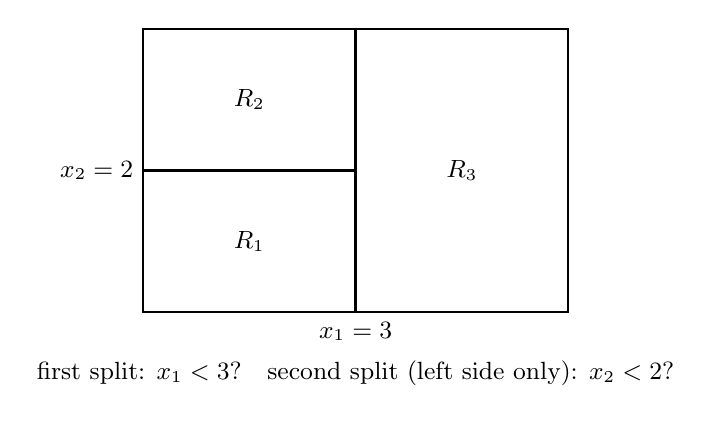
\begin{tikzpicture}[scale=0.9, font=\small]
\draw[thick] (0,0) rectangle (6,4);
\draw[thick] (3,0) -- (3,4);
\draw[thick] (0,2) -- (3,2);
\node at (1.5,1) {$R_1$};
\node at (1.5,3) {$R_2$};
\node at (4.5,2) {$R_3$};
\node[below] at (3,0) {$x_1=3$};
\node[left] at (0,2) {$x_2=2$};
\node[below] at (3,-0.55) {first split: $x_1<3$?\quad second split (left side only): $x_2<2$?};
\end{tikzpicture}
\end{utpfig}

Axis-aligned rules fit naturally; diagonal boundaries require staircases of splits.

\section{Regression trees}

Regression trees choose splits that reduce within-node variance. Each leaf predicts its training-label mean, producing a piecewise-constant function.

\begin{workedexample}
Labels $\{2,3,10,11\}$ have mean $6.5$ and variance $16.25$. Splitting into $\{2,3\}$ and $\{10,11\}$ reduces weighted variance to $0.25$; leaves predict $2.5$ and $10.5$.
\end{workedexample}

Leaf means stay within the training-label range: ordinary regression trees do not extrapolate beyond observed labels.

\section{Stopping and pruning}

Unrestricted growth can produce pure leaves and memorize observations. Use two complementary controls:

\begin{utptable}
\renewcommand{\arraystretch}{1.16}
\setlength{\tabcolsep}{5pt}
\begin{tabularx}{\linewidth}{@{}>{\footnotesize\bfseries\leavevmode\color{UTPNavy}}m{0.22\linewidth}>{\footnotesize}m{0.40\linewidth}>{\footnotesize}X@{}}
\toprule
\rowcolor{UTPPaleBlue!92}
\utpth{Method} & \utpth{How it works} & \utpth{Trade-off} \\
\midrule
Pre-pruning (early stopping) & Refuse to grow past limits set in advance: a maximum depth, a minimum number of observations required to split a node or to sit in a leaf, or a minimum impurity decrease. & Simple and fast; the limits are hyperparameters tuned on validation data. \\
Post-pruning & Grow a deliberately large tree first, then cut back branches whose contribution does not justify their complexity. \term{Cost-complexity pruning} charges a penalty $\alpha$ per leaf and keeps the subtree that best trades training fit against size; $\alpha$ is chosen by cross-validation. & Growing and then cutting can rescue good splits that become visible only after a mediocre one, which early stopping would never discover. \\
\bottomrule
\end{tabularx}
\end{utptable}

\section{Depth: the dial between too simple and memorized}

Tree depth controls the bias--variance trade-off from \secref{sec:bias-variance}.

\begin{utpfig}[Depth and the bias--variance trade-off]{Tree depth versus error. Training error keeps falling as the tree deepens, while validation error is lowest at a moderate depth: stop there.}{fig:tree-depth}
\begin{tikzpicture}
\begin{axis}[
  width=0.68\linewidth, height=4.5cm, axis lines=left,
  title style={font=\small\bfseries\color{UTPNavy}}, title={Tree depth versus error},
  xlabel={max\_depth}, ylabel={Error},
  label style={font=\scriptsize\color{UTPMuted}}, tick label style={font=\scriptsize\color{UTPMuted}},
  legend style={font=\scriptsize,draw=none,fill=none,at={(0.98,0.96)},anchor=north east},
  xmin=0.5, xmax=16, ymin=0, ymax=0.45
]
\addplot[UTPBlue,very thick,mark=*,mark size=1.3pt] coordinates
  {(1,0.34)(2,0.26)(3,0.20)(4,0.16)(6,0.10)(8,0.05)(10,0.02)(12,0.005)(15,0.0)};
\addlegendentry{training error}
\addplot[UTPRed,very thick,mark=square*,mark size=1.3pt] coordinates
  {(1,0.36)(2,0.29)(3,0.24)(4,0.21)(6,0.20)(8,0.23)(10,0.27)(12,0.30)(15,0.33)};
\addlegendentry{validation error}
\draw[UTPGreen,thick,dashed] (axis cs:5,0) -- (axis cs:5,0.45);
\node[font=\scriptsize\color{UTPGreen},anchor=west] at (axis cs:5.4,0.41) {stop here};
\end{axis}
\end{tikzpicture}
\end{utpfig}

\subsection{The controls that limit growth}

\begin{utptable}
\begin{tabularx}{\linewidth}{@{}>{\bfseries\leavevmode\color{UTPNavy}\ttfamily}m{0.25\linewidth}X@{}}
\toprule
\rowcolor{UTPPaleBlue!92}
\utpth{Setting} & \utpth{What it does} \\
\midrule
max\_depth & Hard limit on how many questions can be asked in a row. \\
min\_samples\_split & Refuse to split a node holding fewer than this many rows. \\
min\_samples\_leaf & Every final leaf must contain at least this many rows. \\
max\_leaf\_nodes & Cap the total number of leaves. \\
ccp\_alpha & Cost-complexity pruning: grow fully, then prune back. \\
class\_weight & Make rare-class rows count for more. \\
\bottomrule
\end{tabularx}
\end{utptable}

\subsection{Cost-complexity pruning, properly}

Grow the tree until every leaf is pure or tiny. Then define, for a penalty $\alpha\ge0$, the score
\[
  \text{(training impurity of the subtree)}+\alpha\times\text{(number of leaves)}.
\]
Increasing $\alpha$ trades fit for fewer leaves along a nested pruning path. Cross-validate \texttt{ccp\_alpha}; unlike a uniform depth limit, pruning retains detail where useful.

\section{Strengths, limitations, and practical notes}

\begin{itemize}
  \item \term{Interpretability:} the model \emph{is} an explanation; individual predictions can be justified by reading off the path.
  \item \term{Preprocessing:} numerical trees need no scaling; categorical and missing-value handling depends on the implementation.
  \item \term{Nonlinearity for free:} interactions and thresholds emerge automatically, with no feature engineering.
  \item \term{Instability:} small data changes can alter early splits and whole subtrees, motivating the ensembles in \chapref{ch:ensembles}.
  \item \term{Feature importance:} use the interpretation and bias cautions in \secref{sec:tree-feature-importance}.
\end{itemize}

\begin{keyidea}
Trees learn readable nonlinear rules through impurity reduction. Their instability also makes them useful base learners for ensembles.
\end{keyidea}

\begin{modelcard}{Decision Trees - Quick Guide}
\begin{tabularx}{\linewidth}{@{}>{\bfseries\leavevmode\color{UTPNavy}}p{0.24\linewidth}X@{}}
Best when & Nonlinear rules, interactions, mixed feature scales, and human-readable if-then paths are useful. \cr
Preprocessing & Usually no scaling is needed; categories still need a supported representation; missing-value handling depends on the implementation. \cr
Main controls & Maximum depth, minimum samples per split/leaf, maximum leaf nodes, and pruning strength. \cr
Strengths & Handles nonlinear relationships and interactions; predictions are easy to trace through a small tree. \cr
Watch for & High variance, unstable splits, misleading feature importance, and blocky extrapolation. \cr
\end{tabularx}
\end{modelcard}

\section{Interpreting a fitted tree}

Inspect paths and leaf counts. Lab~3's Titanic tree splits first on \texttt{Sex}, then \texttt{Age} for men and \texttt{Pclass} for women.

\begin{keyidea}
The printed paths are the model's actual rules, not a post-hoc approximation. Readability alone does not establish fairness, causality, stability, or safety.
\end{keyidea}

\section{Feature importance, and why to distrust it}
\label{sec:tree-feature-importance}

\term{Impurity importance} sums a feature's impurity reductions. Two cautions:

\begin{itemize}
  \item Many candidate thresholds can inflate importance, favoring continuous features over binary ones.
  \item Correlated features can substitute for one another, making importance unstable.
\end{itemize}

\term{Permutation importance} is the safer alternative: shuffle one feature's values in the validation data and measure how much the score drops. A large drop means this fitted model relied on that column. It is computed on held-out rows, so it also reflects generalization rather than training fit.

\begin{keyidea}
Feature importance describes which columns this fitted model used. Apply the general association-versus-causation rule from \secref{sec:correlation}; importance is not causal evidence.
\end{keyidea}

\begin{debugtask}
A depth-20 tree has nearly perfect training accuracy and unstable feature importance across random splits. Diagnose the likely failure mode, then compare depth 2, 5, and 20 using identical validation folds and a sealed test set.
\end{debugtask}

\begin{decisionmemo}
Choose between a shallow single tree and a random forest for a decision that must be explained to a nontechnical reviewer. Your memo must separate predictive performance from interpretability and state what level of performance loss, if any, you would accept for the simpler model.
\end{decisionmemo}

\begin{quickcheck}
\begin{enumerate}
  \item What does a decision-tree split try to improve at each node?
  \item Why can an unconstrained tree achieve excellent training performance yet generalize poorly?
  \item Why are ordinary decision trees largely insensitive to monotonic rescaling of a numerical feature?
\end{enumerate}
\end{quickcheck}

\chapter{Ensemble Methods}
\label{ch:ensembles}

\chapterguide%
  {Decision trees from \chapref{ch:decision-trees} and the bias--variance/model-selection ideas from \chapref{ch:training}. The variance framework is referenced rather than retaught.}
  {compare bagging, forests, boosting, voting, and stacking; validate diversity and complexity gains.}

An \term{ensemble} combines models whose errors differ, allowing mistakes to partly cancel. Random forests and boosted trees are strong tabular candidates, but validation and operational constraints determine suitability.

\section{Why averaging helps}

Averaging reduces variance when errors are not perfectly correlated.

For $B$ models with error variance $\sigma^2$, independent errors give average variance $\sigma^2/B$. With average pairwise correlation $\rho$, it is approximately
\[
  \rho\,\sigma^2+\frac{(1-\rho)}{B}\,\sigma^2 .
\]
Adding models reduces the second term, not the correlation floor. \term{Bagging} creates diversity through independent fits on perturbed data; \term{boosting} adds sequential corrections.

\begin{intuition}
A large committee helps only if members bring different errors. Repeating the same view adds little information.
\end{intuition}

\section{Bagging: bootstrap aggregating}

Bagging fits learners to \term{bootstrap samples}: $n$ draws with replacement. Each sample omits about $37\%$ of rows, since $(1-1/n)^n\approx e^{-1}$. Deep trees are common base learners; combine predictions by voting or averaging.

\begin{utpfig}[Bagging]{Bagging. Each tree is fitted to its own bootstrap sample of the training data, and their predictions are combined by voting or averaging.}{fig:bagging}
\begin{tikzpicture}[
  font=\small,
  box/.style={draw, rounded corners=2pt, align=center,
              minimum height=2.2em, minimum width=6.4em, inner sep=3pt, fill=gray!10},
  arr/.style={-{Stealth[length=2mm]}, thick}
]
\node[box] (data) {training data\\($n$ observations)};
\node[box, right=1.05cm of data, yshift=1.35cm] (s1) {bootstrap\\sample 1};
\node[box, right=1.05cm of data] (s2) {bootstrap\\sample 2};
\node[box, right=1.05cm of data, yshift=-1.35cm] (s3) {bootstrap\\sample $B$};
\node[box, right=1.05cm of s1] (t1) {tree 1};
\node[box, right=1.05cm of s2] (t2) {tree 2};
\node[box, right=1.05cm of s3] (t3) {tree $B$};
\node[box, right=1.05cm of t2] (agg) {vote /\\average};
\draw[arr] (data) -- (s1);
\draw[arr] (data) -- (s2);
\draw[arr] (data) -- (s3);
\draw[arr] (s1) -- (t1);
\draw[arr] (s2) -- (t2);
\draw[arr] (s3) -- (t3);
\draw[arr] (t1) -- (agg);
\draw[arr] (t2) -- (agg);
\draw[arr] (t3) -- (agg);
\node at ($(s2)!0.5!(s3)$) {$\vdots$};
\node at ($(t2)!0.5!(t3)$) {$\vdots$};
\end{tikzpicture}
\end{utpfig}

Each row can be predicted by the trees that never saw it; the resulting \term{out-of-bag (OOB)} score is a free validation estimate. Use it as a validation signal for choosing settings, not as a replacement for the final test.

\section{Random forests}
\label{sec:random-forest}

A \term{random forest} adds random feature subsets at each split, reducing correlation between bagged trees. $\sqrt p$ is a common classification starting point; validate feature fractions for regression and other settings.

Practical profile:

\begin{itemize}
  \item \term{Key hyperparameters:} the number of trees $B$ (more trees make the average steadier until the gain flattens out), the number of features tried per split, and tree depth or minimum leaf size.
  \item \term{Little tuning required:} sensible defaults perform well, which makes random forests the standard ``strong model with ten minutes of effort'' on tabular data.
  \item \term{Extras:} OOB error estimates and feature-importance rankings come nearly free; apply the importance caveat from \secref{sec:tree-feature-importance}.
  \item \term{Costs:} the model is large, slower to predict than a single tree, and no longer readable as rules.
\end{itemize}

\subsection{Extra Trees: randomize the split thresholds too}
\label{sec:extra-trees}

\term{Extremely Randomized Trees} (Extra Trees) go one step further than a forest: at each split they draw the candidate thresholds at random instead of searching for the best one, and by default they use the whole training set rather than a bootstrap sample. The extra randomness lowers variance and training time at the cost of a little bias.

Compare Extra Trees with Random Forest under the same folds and metric. Neither is universally better; the useful lesson is that both trade individual-tree strength for diversity across the ensemble.

\section{Boosting: learning from mistakes}

Boosting adds \term{weak learners}, often shallow trees, in sequence to correct the current ensemble. Unlike independent bagging, each fit depends on previous predictions.

\begin{utptable}
\begin{tabular}{@{}p{0.26\linewidth}p{0.31\linewidth}p{0.31\linewidth}@{}}
\toprule
\rowcolor{UTPPaleBlue!92}
\utpth{} & \utpth{Bagging / random forest} & \utpth{Boosting} \\
\midrule
Training & Parallel, independent & Sequential, each model depends on the last \\
Base models & Fully grown, low-bias, high-variance trees & Shallow, high-bias, low-variance trees \\
Main effect & Reduces variance & Reduces bias (and variance via shrinkage) \\
Overfitting risk & Low; robust to noise & Real; needs a learning rate and early stopping \\
Tuning effort & Small & Moderate to large \\
\bottomrule
\end{tabular}
\end{utptable}

\subsection{AdaBoost: reweight the hard cases}
\label{sec:adaboost}

AdaBoost repeatedly increases the weights of misclassified observations:

\begin{enumerate}
  \item Start with equal weights $w_i=1/n$.
  \item Fit a weak learner $h_m$ to the weighted data and compute its weighted error rate $\varepsilon_m$.
  \item Give the learner a say proportional to its quality:
  \[
    \alpha_m=\tfrac{1}{2}\ln\frac{1-\varepsilon_m}{\varepsilon_m}.
  \]
  \item Multiply misclassified weights by $e^{\alpha_m}$ and correct weights by $e^{-\alpha_m}$, then renormalize.
  \item After $M$ rounds, predict with the weighted vote $\operatorname{sign}\!\left(\sum_m\alpha_m h_m(\bm{x})\right)$.
\end{enumerate}

At $\varepsilon_m=0.3$, $\alpha_m\approx0.42$, multiplying misclassified weights by about $1.5$. A chance learner ($\varepsilon_m=0.5$) gets no vote. Repeated emphasis on mislabeled cases makes AdaBoost sensitive to label noise.

\subsection{Gradient boosting: fit the residuals}
\label{sec:gradient-boosting}

Gradient boosting fits $h_m$ to the negative loss gradient at current predictions. For squared loss this is the residual $y_i-F_{m-1}(\bm x_i)$. Update by
\[
  F_m(\bm{x})
  =F_{m-1}(\bm{x})+\nu\,h_m(\bm{x}),
  \qquad 0<\nu\leq 1.
\]
The learning rate $\nu$ scales each correction. Tune it jointly with tree count, using validation or early stopping.

\begin{workedexample}
For $y=(3,5,8,10)$, $F_0=6.5$ gives residuals $(-3.5,-1.5,1.5,3.5)$. A stump grouping the first two and last two rows predicts residual means $-2.5$ and $2.5$. With $\nu=0.5$,
\[
  F_1=(6.5-1.25,\;6.5-1.25,\;6.5+1.25,\;6.5+1.25)
  =(5.25,\,5.25,\,7.75,\,7.75),
\]
and residuals become $(-2.25,-0.25,0.25,2.25)$. Later rounds add further corrections.
\end{workedexample}

\begin{utpfig}[Gradient boosting shrinks the residuals]{Gradient boosting on the worked example. Round 0 predicts the mean; one stump with learning rate $\nu=0.5$ shrinks every residual towards zero.}{fig:boosting-residuals}
\begin{tikzpicture}[
  x=1cm, y=1cm, font=\small,
  ax/.style={draw=UTPMuted!55,semithick},
  obs/.style={circle,fill=UTPNavy,inner sep=1.5pt},
  fit/.style={draw=UTPBlue,line width=1.1pt},
  resid/.style={-{Stealth[length=1.7mm]},draw=UTPRed,semithick},
  rl/.style={font=\tiny\color{UTPRed}},
  hd/.style={font=\small\bfseries\color{UTPNavy}},
  yl/.style={font=\tiny\color{UTPMuted},anchor=east}]

% ---------- round 0: predict the mean ----------
\node[hd] at (1.9,4.35) {Round 0: predict the mean};
\draw[ax] (0.30,0) -- (0.30,3.95);
\draw[ax] (0.30,0) -- (3.55,0);
\foreach \v/\cy in {3/0.42, 5/1.26, 8/2.52, 10/3.36} \node[yl] at (0.22,\cy) {\v};

\draw[fit] (0.45,1.89) -- (3.35,1.89);
\node[font=\tiny\color{UTPBlue},anchor=west] at (3.40,1.89) {$F_0=6.5$};

\draw[resid] (0.70,1.89) -- (0.70,0.50);
\draw[resid] (1.50,1.89) -- (1.50,1.34);
\draw[resid] (2.30,1.89) -- (2.30,2.44);
\draw[resid] (3.10,1.89) -- (3.10,3.28);
\node[rl,anchor=west] at (0.78,1.16) {$-3.5$};
\node[rl,anchor=west] at (1.58,1.62) {$-1.5$};
\node[rl,anchor=west] at (2.38,2.16) {$+1.5$};
\node[rl,anchor=west] at (3.18,2.62) {$+3.5$};

\foreach \cx/\cy in {0.70/0.42, 1.50/1.26, 2.30/2.52, 3.10/3.36}
  \node[obs] at (\cx,\cy) {};

% ---------- round 1: add half of a stump ----------
\begin{scope}[xshift=7.0cm]
\node[hd] at (1.9,4.35) {After round 1, with $\nu=0.5$};
\draw[ax] (0.30,0) -- (0.30,3.95);
\draw[ax] (0.30,0) -- (3.55,0);
\foreach \v/\cy in {3/0.42, 5/1.26, 8/2.52, 10/3.36} \node[yl] at (0.22,\cy) {\v};

\draw[fit] (0.45,1.365) -- (1.90,1.365);
\draw[fit] (1.90,2.415) -- (3.35,2.415);
\draw[fit,dashed] (1.90,1.365) -- (1.90,2.415);
\node[font=\tiny\color{UTPBlue},anchor=west] at (3.40,2.415) {$F_1$};

\draw[resid] (0.70,1.365) -- (0.70,0.50);
\draw[resid] (1.50,1.365) -- (1.50,1.34);
\draw[resid] (2.30,2.415) -- (2.30,2.44);
\draw[resid] (3.10,2.415) -- (3.10,3.28);
\node[rl,anchor=west] at (0.78,0.86) {$-2.25$};
\node[rl,anchor=west] at (1.58,1.30) {$-0.25$};
\node[rl,anchor=west] at (2.38,2.05) {$+0.25$};
\node[rl,anchor=west] at (3.18,2.85) {$+2.25$};

\foreach \cx/\cy in {0.70/0.42, 1.50/1.26, 2.30/2.52, 3.10/3.36}
  \node[obs] at (\cx,\cy) {};
\end{scope}

\node[font=\scriptsize\color{UTPInk},align=center,text width=12.5cm] at (5.4,-0.85)
  {The stump is never fitted to the labels --- it is fitted to the red arrows.
   One split separates the first two observations from the last two and predicts
   their residual means, $-2.5$ and $+2.5$; the learning rate admits only half
   of that, so every residual shrinks but none is erased. A hundred such
   corrections trace the data closely.};

\end{tikzpicture}
\end{utpfig}

\begin{intuition}
Gradient boosting fits corrections; AdaBoost reweights mistakes. Both train sequentially.
\end{intuition}

\subsection{Modern gradient-boosting libraries}

Three refinements of gradient boosting dominate practical work; all keep the algorithm above and add engineering and regularization:

\begin{utptable}
\begin{tabularx}{\linewidth}{@{}>{\bfseries\leavevmode\color{UTPNavy}}m{0.18\linewidth}m{0.46\linewidth}X@{}}
\toprule
\rowcolor{UTPPaleBlue!92}
\utpth{Library} & \utpth{Distinctive approach} & \utpth{Practical strength} \\
\midrule
XGBoost & Adds explicit regularization of tree size and leaf values to the objective and uses second-derivative information for better splits. & Popularized the modern toolkit, including early stopping and column subsampling. \\
LightGBM & Grows trees leaf-wise instead of level-wise and buckets feature values into histograms. & Extremely fast on large datasets. \\
CatBoost & Handles categorical features natively with label statistics computed in a careful order to avoid leakage. & Notably strong when the data contains many categorical columns. \\
\bottomrule
\end{tabularx}
\end{utptable}

The hyperparameters that matter most, in rough order: number of trees (via early stopping), learning rate, tree depth or leaf count, and the row/column subsampling fractions.

\section{Bagging and boosting, side by side}
\label{sec:bagging-vs-boosting}

Bagging fits independently and can run in parallel; boosting fits sequential corrections.

\begin{utpfig}[Bagging and boosting side by side]{Bagging fits trees in parallel on independent samples and reduces variance; boosting fits them in sequence, each correcting the remaining errors, and reduces bias.}{fig:bagging-boosting}
\begin{tikzpicture}[
  node distance=0.3cm and 0.55cm,
  t/.style={draw=UTPBlue,fill=UTPPaleBlue,rounded corners=1.2mm,minimum width=1.45cm,minimum height=0.55cm,align=center,font=\scriptsize\bfseries\color{UTPNavy}},
  tb/.style={draw=UTPOrange,fill=UTPPaleOrange,rounded corners=1.2mm,minimum width=1.45cm,minimum height=0.55cm,align=center,font=\scriptsize\bfseries\color{UTPNavy}},
  d/.style={draw=UTPMuted,fill=UTPPaleGray,rounded corners=1.2mm,minimum width=1.1cm,minimum height=0.5cm,align=center,font=\tiny\color{UTPNavy}},
  agg/.style={draw=UTPGreen,fill=UTPPaleTeal,rounded corners=1.5mm,minimum width=1.5cm,minimum height=1.9cm,align=center,font=\scriptsize\bfseries\color{UTPNavy}},
  result/.style={draw=UTPGreen,fill=UTPPaleTeal,rounded corners=1.2mm,minimum width=1.15cm,minimum height=0.55cm,align=center,font=\scriptsize\bfseries\color{UTPNavy}},
  arr/.style={-{Stealth[length=1.8mm]},thick,draw=UTPTeal},
  arro/.style={-{Stealth[length=1.8mm]},thick,draw=UTPOrange}
]
% ---- bagging ----
\node[font=\small\bfseries\color{UTPNavy}] (hb) at (0,2.55) {Bagging: parallel and independent};
\node[d] (d1) at (-1.3,1.85) {sample 1};
\node[d] (d2) at (-1.3,1.15) {sample 2};
\node[d] (d3) at (-1.3,0.45) {sample 3};
\node[t] (t1) at (0.55,1.85) {tree 1};
\node[t] (t2) at (0.55,1.15) {tree 2};
\node[t] (t3) at (0.55,0.45) {tree 3};
\node[agg] (av) at (2.5,1.15) {average\\or vote};
\draw[arr] (d1)--(t1); \draw[arr] (d2)--(t2); \draw[arr] (d3)--(t3);
\draw[arr] (t1)--(av); \draw[arr] (t2)--(av); \draw[arr] (t3)--(av);
\node[font=\scriptsize\itshape\color{UTPMuted}] at (0.6,-0.2) {reduces variance};
% ---- boosting ----
\node[font=\small\bfseries\color{UTPNavy}] (hs) at (8.85,2.55) {Boosting: sequential and corrective};
\node[tb] (b1) at (5.75,1.45) {tree 1};
\node[tb] (b2) at (8.05,1.45) {tree 2};
\node[tb] (b3) at (10.35,1.45) {tree 3};
\node[result] (sum) at (12.15,1.45) {weighted\\sum};
\draw[arro] (b1.east)--(b2.west);
\draw[arro] (b2.east)--(b3.west);
\draw[arro] (b3.east)--(sum.west);
\node[font=\tiny\color{UTPRed},align=center] at (6.90,0.88)
  {fit remaining\\errors};
\node[font=\tiny\color{UTPRed},align=center] at (9.20,0.88)
  {fit remaining\\errors};
\node[font=\scriptsize\itshape\color{UTPMuted}] at (8.85,-0.2) {reduces bias};
\end{tikzpicture}
\end{utpfig}

\begin{keyidea}
Bagging often uses deep trees; boosting often uses shallow trees. Validate depth, leaf size, learning rate, and rounds together.
\end{keyidea}

\section{Voting and stacking}

\term{Voting} combines models by majority labels or averaged probabilities. \term{Stacking} trains a \term{meta-model} on base predictions to learn their combination.

Train the meta-model on \term{out-of-fold} base predictions, not predictions fitted to those same rows. Otherwise it learns from overfitted outputs. Linear or logistic meta-models are common.

\section{Practical ensemble workflow}

\begin{itemize}
  \item Want a strong tabular model with minimal fuss? \term{Random forest}.
  \item Chasing the best accuracy and willing to tune? \term{Gradient boosting} with early stopping.
  \item Noisy labels? Prefer forests over AdaBoost-style boosting, or lower the boosting learning rate and depth.
  \item Stack diverse models only when out-of-fold validation justifies the added maintenance.
\end{itemize}

In Lab~3, boosting beats forests on Ames Housing but loses on wine quality. Weigh dataset-specific gains against tuning and runtime.

\begin{keyidea}
Bagging averages varied trees; boosting adds dependent corrections. Judge their gains against latency, interpretability, and maintenance costs.
\end{keyidea}

\begin{modelcard}{Tree Ensembles - Quick Guide}
\begin{tabularx}{\linewidth}{@{}>{\bfseries\leavevmode\color{UTPNavy}}m{0.22\linewidth}X X@{}}
\toprule
\rowcolor{UTPPaleBlue!92}
\utpth{} & \utpth{Random forest} & \utpth{Gradient boosting} \\
\midrule
Core idea & Average many varied trees & Add shallow trees sequentially to repair errors \cr
Usually strong for & Reliable general-purpose tabular prediction & High predictive accuracy on structured/tabular data \cr
Main controls & Number of trees, sampled features, depth, leaf size & Number of trees, learning rate, depth, subsampling \cr
Main risks & Large models, less transparent than one tree & Overfitting through too many rounds, sensitive tuning, slower training \cr
\bottomrule
\end{tabularx}
\end{modelcard}

\subsection{Controls worth tuning}

Random forests are usually forgiving: start with enough trees for stable averages, then control individual-tree complexity with depth, leaf size, and the number of features considered at each split. Gradient boosting is more sensitive because learning rate and number of rounds trade off directly. The table below is a practical starting range, not a universal recipe.

\begin{pitfall}
Early-stopping validation must preserve time or group structure. Supply an appropriately separated validation set or tune rounds with structure-preserving folds.
\end{pitfall}

\begin{utptable}
\begin{tabularx}{\linewidth}{@{}>{\bfseries\leavevmode\color{UTPNavy}\ttfamily}m{0.21\linewidth}m{0.16\linewidth}X@{}}
\toprule
\rowcolor{UTPPaleBlue!92}
\utpth{Setting} & \utpth{Try} & \utpth{Effect} \\
\midrule
learning\_rate & 0.01--0.1 & Smaller learns more carefully; needs more trees. \\
n\_estimators & 300--2000 & With early stopping, set it generously. \\
max\_depth & 3--8 & Deeper catches interactions but overfits sooner. \\
subsample & 0.6--1.0 & Row sampling; adds randomness, fights overfitting. \\
colsample\_bytree & 0.6--1.0 & Column sampling; same idea, per feature. \\
reg\_lambda & 0--10 & Extra penalty on leaf values. \\
\bottomrule
\end{tabularx}
\end{utptable}

\subsection{When combining model families helps}

\begin{intuition}
Stacking can adapt model weights to different cases, but the extra layer needs sufficient data and out-of-fold training.
\end{intuition}

\begin{pitfall}
Combine individually useful, non-redundant models, such as a linear model and a forest. Keep the ensemble only if validation gains justify its complexity.
\end{pitfall}

\section{Inspecting ensemble predictions}
\label{sec:ensemble-interpretability}

Use permutation importance (\secref{sec:tree-feature-importance}), partial dependence, or SHAP to describe model behavior, not causal effects.

Correlated features can mask permutation importance. Partial dependence averages predictions as one feature varies, potentially creating implausible combinations.

\subsection{Optional: SHAP for local explanations}

\term{SHAP} (SHapley Additive exPlanations) decomposes a prediction relative to a reference output:
\[
  \hat{y}_i = \mathbb{E}[\hat{y}] + \sum_{j=1}^{p}\phi_{ij}.
\]
$\phi_{ij}$ attributes row $i$'s departure from the reference output. Correlated features can redistribute attribution; check stability.

Apply the association-versus-causation distinction from \secref{sec:correlation}: an explanation can reveal what the model used without proving what would happen under an intervention.

\section{Ensemble comparison at a glance}

\begin{utptable}
\begin{tabularx}{\linewidth}{@{}>{\bfseries\leavevmode\color{UTPNavy}}m{0.22\linewidth}m{0.25\linewidth}X@{}}
\toprule
\rowcolor{UTPPaleBlue!92}
\utpth{Method} & \utpth{What changes from one tree} & \utpth{Main reason to try it} \\
\midrule
Bagging & Bootstrap many trees and average/vote & Reduce variance and make a high-variance learner more stable \\
Random Forest & Bagging plus random feature subsets at splits & Make the trees less correlated, so averaging helps more \\
AdaBoost & Train weak learners sequentially with emphasis on previous errors & Reduce bias by focusing later learners on difficult cases \\
Soft voting & Average probabilities from different model families & Combine complementary decision rules rather than many copies of one rule \\
\bottomrule
\end{tabularx}
\end{utptable}

\begin{tryit}
Compare a single tree, a random forest, and a gradient-boosting model with the same cross-validation splits. Record mean validation score, descriptive fold spread, fit time, and prediction time. Decide whether any gain justifies the added cost, then evaluate the locked choice on the test set once.
\end{tryit}

\begin{quickcheck}
\begin{enumerate}
  \item How does bagging reduce variance, and how does boosting differ in the way later learners are constructed?
  \item Why does a random forest consider only a subset of features at many splits?
  \item Why must predictions used to train a stacking meta-model be out-of-fold rather than fitted predictions from the same rows?
\end{enumerate}
\end{quickcheck}

\chapter{Support Vector Machines and Supervised Synthesis}
\label{ch:svm}

\chapterguide%
  {Linear classifiers from \chapref{ch:classification}, model-capacity ideas from \chapref{ch:training}, and dot products/norms from \chapref{ch:linear-algebra}.}
  {explain margins, kernels, scaling, and SVM tuning; compare supervised model families.}

A support vector machine (SVM) chooses a separating boundary with a wide \emph{margin}. The \term{support vectors}, on or inside that margin, determine the fitted boundary.

\section{The widest street}

\begin{utpfig}[The widest street]{The widest street. A hard-margin SVM places the boundary in the middle of the widest margin between the classes; the circled support vectors on its edges determine it.}{fig:svm-margin}
\begin{tikzpicture}[scale=0.85, font=\small]
% class + (filled)
\foreach \p in {(1,1),(2,1.2),(1,2.6),(0.8,1.8),(2.4,0.8)}
  \fill \p circle (2.4pt);
% class - (open)
\foreach \p in {(4,4),(5,3.5),(3.6,4.9),(4.6,4.7),(5.2,2.9)}
  \draw[thick, fill=gray!30] \p circle (2.4pt);
% support vectors
\fill (1.5,2.5) circle (2.4pt);
\draw[thick, fill=gray!30] (2.5,3.5) circle (2.4pt);
\draw[thick, fill=gray!30] (4,2) circle (2.4pt);
\draw (1.5,2.5) circle (5.5pt);
\draw (2.5,3.5) circle (5.5pt);
\draw (4,2) circle (5.5pt);
% lines
\draw[thick] (0,5) -- (5,0)
  node[pos=0.06, right=2pt] {$\bm{w}^{\mathsf T}\bm{x}+b=0$};
\draw[dashed] (0,4) -- (4,0);
\draw[dashed] (0,6) -- (6,0);
% margin arrow
\draw[{Stealth[length=2mm]}-{Stealth[length=2mm]}, thick]
  (3.1,0.9) -- (4.1,1.9) node[midway, below right=-1pt] {margin};
\node[align=left] at (5.35,5.3) {circled points =\\support vectors};
\end{tikzpicture}
\end{utpfig}

\begin{intuition}
A hard-margin SVM builds the widest street between two classes. Points touching its curbs determine the street; distant points do not.
\end{intuition}

\section{The hard-margin objective}

For $y_i\in\{-1,+1\}$, require correctly signed linear scores of magnitude at least one:
\[
  \min_{\bm{w},b}\ \frac{1}{2}\|\bm{w}\|_2^2
  \quad\text{subject to}\quad
  y_i(\bm{w}^{\mathsf T}\bm{x}_i+b)\geq 1 .
\]
The constraint requires the correct sign and score magnitude at least~1. The margin width is $2/\|\bm w\|_2$, so minimizing the norm maximizes that width.

\section{The soft margin: allowing exceptions}

Real classes overlap, so the SVM used in practice permits violations and charges for them:
\[
  \min_{\bm{w},b}\
  \frac{1}{2}\|\bm{w}\|_2^2
  +C\sum_{i=1}^{n}
  \max\!\left(0,\,1-y_i(\bm{w}^{\mathsf T}\bm{x}_i+b)\right).
\]
\term{Hinge loss} is zero beyond the margin and linear within it or on the wrong side. $C$ balances margin width against violations:

\begin{itemize}
  \item \term{Large $C$}: violations cost more; weaker regularization can overfit.
  \item \term{Small $C$}: more violations are tolerated; regularization is stronger.
\end{itemize}

Both SVMs and regularized logistic regression combine loss with an $L_2$ penalty. Hinge loss becomes zero beyond the margin; cross-entropy continues rewarding confidence.

\section{Curved boundaries: mapping up}

Some datasets cannot be separated by any straight line --- but they can be after the features are transformed.

\begin{workedexample}
Let $x\in\{-2,2\}$ be class A and $x\in\{-1,0,1\}$ class B. No single threshold separates them. Map to $\phi(x)=(x,x^2)$:
\begin{utptable}
\begin{tabular}{@{}lccccc@{}}
\toprule
\rowcolor{UTPPaleBlue!92}
\utpth{$x$} & \utpth{$-2$} & \utpth{$-1$} & \utpth{$0$} & \utpth{$1$} & \utpth{$2$} \\
\midrule
$x^2$ & $4$ & $1$ & $0$ & $1$ & $4$ \\
class & A & B & B & B & A \\
\bottomrule
\end{tabular}
\end{utptable}
Class A has height 4 and class B at most 1. The line $x^2=2.5$ separates them, corresponding to two thresholds $|x|=\sqrt{2.5}$ in the original space.
\end{workedexample}

\section{The kernel trick}

Rich feature maps can be expensive or infinite-dimensional. SVM equations use them only through inner products; a \term{kernel function} computes these directly:
\[
  k(\bm{x},\bm{x}')=\phi(\bm{x})^{\mathsf T}\phi(\bm{x}'),
\]
so the mapped features never need to be constructed at all --- this shortcut is the \term{kernel trick}. Standard choices:

\begin{utptable}
\begin{tabular}{@{}lll@{}}
\toprule
\rowcolor{UTPPaleBlue!92}
\utpth{Kernel} & \utpth{Formula} & \utpth{Boundary it produces} \\
\midrule
Linear & $\bm{x}^{\mathsf T}\bm{x}'$ & Straight; fast on huge, sparse data \\
Polynomial & ${(\gamma\,\bm{x}^{\mathsf T}\bm{x}'+r)}^d$ & Curved, degree-$d$ interactions \\
RBF (Gaussian) & $\exp\!\left(-\gamma\|\bm{x}-\bm{x}'\|_2^2\right)$ & Smooth, local, very flexible \\
\bottomrule
\end{tabular}
\end{utptable}

The \term{RBF kernel} measures similarity that decays with distance. Small $\gamma$ gives broad influence and smooth boundaries; large $\gamma$ gives local, flexible boundaries. Tune $C$ and $\gamma$ together on logarithmic grids.

\begin{intuition}
RBF support vectors act as landmarks with distance-decaying influence. The kernel evaluates their similarity without explicitly constructing the feature map.
\end{intuition}

% === VISUAL ADDITION: svm-linear-vs-rbf ===
\subsection{Linear versus RBF boundaries, drawn}

A feature map can make a nonlinear separation linear in the transformed space.

\begin{utpfig}[Linear versus RBF boundaries]{Linear versus RBF boundaries. One straight line cannot put a central region in its own class; an RBF kernel draws a smooth curved boundary that isolates it.}{fig:svm-kernels}
\begin{tikzpicture}[font=\scriptsize]
\begin{scope}
  \draw[draw=UTPMuted!70,fill=white] (0,0) rectangle (4.7,3.8);
  \node[font=\small\bfseries\color{UTPNavy}] at (2.35,4.2) {Linear kernel};
  \foreach \p in {(2.0,1.7),(2.4,1.9),(2.1,2.3),(2.7,2.2),(2.55,1.55)}
    \fill[UTPBlue] \p circle (2.6pt);
  \foreach \p in {(0.65,0.65),(1.0,3.05),(3.75,0.7),(4.0,3.0),(0.55,2.0),(4.15,1.85)}
    \draw[UTPOrange,very thick] \p circle (2.9pt);
  \draw[UTPNavy,very thick] (0.35,2.9) -- (4.35,0.85);
  \node[align=center,text=UTPRed] at (2.35,-0.48)
    {one straight line cannot\\put the center in its own class};
\end{scope}

\begin{scope}[xshift=6.0cm]
  \draw[draw=UTPMuted!70,fill=white] (0,0) rectangle (4.7,3.8);
  \node[font=\small\bfseries\color{UTPNavy}] at (2.35,4.2) {RBF kernel};
  \foreach \p in {(2.0,1.7),(2.4,1.9),(2.1,2.3),(2.7,2.2),(2.55,1.55)}
    \fill[UTPBlue] \p circle (2.6pt);
  \foreach \p in {(0.65,0.65),(1.0,3.05),(3.75,0.7),(4.0,3.0),(0.55,2.0),(4.15,1.85)}
    \draw[UTPOrange,very thick] \p circle (2.9pt);
  \draw[UTPTeal,very thick] (2.35,1.95) ellipse (1.15 and 0.92);
  \node[align=center,text=UTPGreen] at (2.35,-0.48)
    {a smooth curved boundary\\can isolate the local region};
\end{scope}

\node[font=\scriptsize\color{UTPBlue}] at (4.9,4.18) {$\bullet$ class A};
\node[font=\scriptsize\color{UTPOrange}] at (6.65,4.18) {$\circ$ class B};
\end{tikzpicture}
\end{utpfig}

\begin{keyidea}
A kernel changes the representation during fitting; it does not bend an already-trained line afterward.
\end{keyidea}
% === END VISUAL ADDITION ===

\section{What $C$ and $\gamma$ actually do}
\label{sec:svm-controls}

\begin{utpfig}[What C does]{What $C$ does. A small $C$ keeps a wide street and tolerates a stray point; a large $C$ narrows the street and bends to capture it, at the risk of overfitting.}{fig:svm-c}
\begin{tikzpicture}[scale=0.82, every node/.style={font=\scriptsize}]
\begin{scope}
\draw[draw=UTPMuted,fill=white] (0,0) rectangle (3.5,2.8);
\draw[UTPNavy,very thick] (0.3,0.2) -- (3.2,2.6);
\draw[UTPNavy,dashed] (0.05,0.75) -- (2.7,2.95);
\draw[UTPNavy,dashed] (0.75,-0.15) -- (3.5,2.15);
\fill[UTPBlue!12] (0.05,0.75) -- (2.7,2.95) -- (3.5,2.15) -- (0.75,-0.15) -- cycle;
\draw[UTPNavy,very thick] (0.3,0.2) -- (3.2,2.6);
\foreach \p in {(0.5,1.9),(1.0,2.4),(0.35,1.35),(1.5,2.65)} \fill[UTPBlue] \p circle (2.2pt);
\foreach \p in {(2.4,0.5),(2.9,1.0),(3.2,0.4),(1.9,0.25)} \fill[UTPOrange] \p circle (2.2pt);
\fill[UTPOrange] (1.65,1.6) circle (2.2pt);
\node[font=\small\bfseries\color{UTPNavy}] at (1.75,3.15) {small $C$: wide street};
\node[color=UTPMuted,align=center] at (1.75,-0.55) {tolerates the stray point\\simpler, may underfit};
\end{scope}
\begin{scope}[xshift=4.6cm]
\draw[draw=UTPMuted,fill=white] (0,0) rectangle (3.5,2.8);
\fill[UTPRed!10] (0.35,0.95) -- (2.15,2.9) -- (2.6,2.5) -- (0.8,0.55) -- cycle;
\draw[UTPRed,very thick,rounded corners=2pt] (0.2,0.5) -- (1.2,1.3) -- (1.45,1.85) -- (2.0,2.2) -- (2.6,2.8);
\foreach \p in {(0.5,1.9),(1.0,2.4),(0.35,1.35),(1.5,2.65)} \fill[UTPBlue] \p circle (2.2pt);
\foreach \p in {(2.4,0.5),(2.9,1.0),(3.2,0.4),(1.9,0.25)} \fill[UTPOrange] \p circle (2.2pt);
\fill[UTPOrange] (1.65,1.6) circle (2.2pt);
\draw[UTPRed,very thick] (1.4,1.45) circle (0.32);
\node[font=\small\bfseries\color{UTPNavy}] at (1.75,3.15) {large $C$: narrow street};
\node[color=UTPMuted,align=center] at (1.75,-0.55) {bends to capture it\\complex, may overfit};
\end{scope}
\end{tikzpicture}
\end{utpfig}

\begin{utptable}
\begin{tabularx}{\linewidth}{@{}>{\bfseries\leavevmode\color{UTPNavy}}m{0.10\linewidth}m{0.27\linewidth}X@{}}
\toprule
\rowcolor{UTPPaleBlue!92}
\utpth{Dial} & \utpth{Plain meaning} & \utpth{Turn it up when} \\
\midrule
$C$ & How badly you want to avoid mistakes on the training data & The model underfits; the boundary is too simple \\
$\gamma$ & How far a single training point's influence reaches & The boundary needs to be more local and wiggly \\
\bottomrule
\end{tabularx}
\end{utptable}

\begin{analogy}
$C$ is a strictness setting for a teacher marking homework. A low $C$ teacher accepts that a few students will get things wrong and teaches a general rule. A high $C$ teacher insists that every single student's answer be accommodated, and ends up teaching a rule so contorted that nobody can apply it to a new question.

$\gamma$ is the radius of each training point's voice. Low $\gamma$ means every point is heard across the whole room, producing a smooth global boundary. High $\gamma$ means each point is only heard by its immediate neighbors, producing islands around individual examples.
\end{analogy}

\section{Multiclass SVMs and support vector regression}

Multiclass reductions include \term{one-vs-rest} ($K$ classifiers) and \term{one-vs-one} (one per class pair, combined by voting).

\term{Support vector regression (SVR)} recycles the margin idea for numeric labels: build a tube of half-width $\varepsilon$ around the prediction and charge nothing for points inside it, using the $\varepsilon$-insensitive loss $\max(0,\,|y-f(\bm{x})|-\varepsilon)$. Only points on or outside the tube become support vectors, giving a sparse, outlier-tolerant regressor with the full kernel toolbox available.

\section{Practical notes}

\begin{itemize}
  \item \term{Scale the features.} Apply the distance-geometry rule from \secref{sec:scaling}.
  \item \term{Tune $C$ (and $\gamma$)} by cross-validation over logarithmic grids such as $10^{-2},\ldots,10^{3}$.
  \item \term{Scale limits:} kernel SVMs suit small-to-medium datasets; linear SVMs suit high-dimensional text. Large datasets may favor linear models or ensembles.
  \item \term{Probabilities are not native.} SVMs output scores and margins; if calibrated probabilities are needed, apply and validate a calibration step (\chapref{ch:evaluation}).
\end{itemize}

\section{Choosing a supervised model}
\label{sec:supervised-model-choice}

\begin{utptable}
\begin{tabular}{@{}p{0.19\linewidth}p{0.36\linewidth}p{0.36\linewidth}@{}}
\toprule
\rowcolor{UTPPaleBlue!92}
\utpth{Model} & \utpth{Useful strengths} & \utpth{Important limitations} \\
\midrule
Linear regression & Interpretable, fast, the standard first baseline & Linear relationships only; sensitive to outliers \\
Ridge / lasso & Controls overfitting; lasso selects features & Still linear; needs feature scaling \\
Logistic regression & Strong probability baseline, convex training, interpretable odds & Linear boundary; calibration still needs checking \\
LDA / QDA & Fast, stable on small data & Gaussian class assumptions \\
$k$-NN & No training, flexible boundaries & Slow at prediction; scale- and dimension-sensitive \\
Naive Bayes & Very fast, strong text baseline & Independence and calibration caveats (\secref{sec:naive-bayes}) \\
Decision tree & Readable rules, no scaling, mixed data & Unstable; overfits without pruning \\
Random forest & Robust, accurate, minimal tuning & Larger, slower, less transparent \\
Gradient boosting & Often a very strong tabular benchmark & Needs careful tuning and early stopping \\
SVM & Margins and kernels; strong in high dimensions & Scaling required; slow on very large data \\
\bottomrule
\end{tabular}
\end{utptable}

Start with regularized linear models; add complexity only for validated gains. In Lab~3, a tuned SVM reaches test AUC 0.997 versus 0.986--0.992 for simpler KNN/naive Bayes fits.

\begin{keyidea}
SVMs illustrate two reusable ideas: wide margins control complexity, and kernels allow linear methods to express nonlinear boundaries.
\end{keyidea}

\begin{modelcard}{Support Vector Machines - Quick Guide}
\begin{tabularx}{\linewidth}{@{}>{\bfseries\leavevmode\color{UTPNavy}}p{0.24\linewidth}X@{}}
Best when & The dataset is small to medium sized, features are informative, and a strong margin-based boundary is useful. \cr
Preprocessing & Standardize numerical features; encode categories; remove clearly irrelevant features when justified by the validated workflow in \secref{sec:feature-selection}. \cr
Main controls & $C$ for margin violations; kernel choice; $\gamma$ for RBF-kernel reach; $\varepsilon$ for SVR. \cr
Strengths & Effective in high-dimensional spaces and flexible through kernels. \cr
Watch for & Slow training on very large datasets, sensitive scale, difficult probability interpretation, and expensive kernel tuning. \cr
\end{tabularx}
\end{modelcard}

\labsection{3}{Supervised learning II: model families}{sec:lab03-supervised-models}

\begin{labproject}{Neighbours, naive Bayes, trees, ensembles, and support vector machines on one workflow}
\textbf{Coverage.} Chapters~\ref{ch:knn-nb}--\ref{ch:svm}.\\
\textbf{Goal.} Compare model families under Lab~2's fixed validation workflow; inspect boundaries, tree depth, ensemble gains, and SVM tuning.

\medskip\noindent\textbf{Setup.}\par
\begin{lstlisting}[style=utppython]
from pathlib import Path

import joblib
import matplotlib.pyplot as plt
import numpy as np
import pandas as pd
from sklearn.compose import ColumnTransformer
from sklearn.ensemble import GradientBoostingRegressor, RandomForestRegressor
from sklearn.impute import SimpleImputer
from sklearn.inspection import DecisionBoundaryDisplay, permutation_importance
from sklearn.linear_model import LogisticRegression
from sklearn.metrics import accuracy_score, mean_absolute_error, mean_squared_error, roc_auc_score
from sklearn.model_selection import (
    GridSearchCV, KFold, StratifiedKFold, cross_val_score, train_test_split,
)
from sklearn.naive_bayes import GaussianNB
from sklearn.neighbors import KNeighborsClassifier
from sklearn.pipeline import Pipeline
from sklearn.preprocessing import OneHotEncoder, StandardScaler
from sklearn.svm import SVC
from sklearn.tree import DecisionTreeClassifier, export_text, plot_tree

PROJECT_ROOT = Path.cwd().parent
DATA = PROJECT_ROOT / "all_datasets"
MODELS = PROJECT_ROOT / "models"
MODELS.mkdir(exist_ok=True)
\end{lstlisting}

\medskip\noindent\textbf{Part A --- KNN versus Gaussian naive Bayes.}\par

KNN votes among standardized neighbors; Gaussian naive Bayes combines per-feature Gaussian likelihoods and class priors.

\begin{lstlisting}[style=utppython]
cancer = pd.read_csv(DATA / "breast_cancer_dataset.csv")

X_c = cancer.drop(columns=["id", "diagnosis", "Unnamed: 32"], errors="ignore")
y_c = (cancer["diagnosis"] == "M").astype(int)

Xc_train, Xc_valid, yc_train, yc_valid = train_test_split(
    X_c, y_c, test_size=0.25, random_state=42, stratify=y_c
)
\end{lstlisting}

$k$ is a hyperparameter, so it is chosen by cross-validation inside the training partition. Small $k$ follows every local quirk (low bias, high variance); large $k$ smooths everything (high bias, low variance).

\begin{lstlisting}[style=utppython]
cv = StratifiedKFold(n_splits=5, shuffle=True, random_state=42)
k_values = [1, 3, 5, 7, 11, 21]
cv_scores = {}

for k in k_values:
    candidate = Pipeline([
        ("scale", StandardScaler()),
        ("model", KNeighborsClassifier(n_neighbors=k, weights="distance")),
    ])
    scores = cross_val_score(candidate, Xc_train, yc_train, cv=cv, scoring="roc_auc")
    cv_scores[k] = scores.mean()
    print(f"k={k:2d}  cross-validated ROC AUC = {scores.mean():.3f}")

best_k = max(cv_scores, key=cv_scores.get)
print("selected k:", best_k)

plt.figure(figsize=(5, 3.2))
plt.plot(k_values, [cv_scores[k] for k in k_values], marker="o")
plt.axvline(best_k, linestyle="--", color="grey")
plt.xlabel("k (number of neighbours)")
plt.ylabel("Cross-validated ROC AUC")
plt.title("Choosing k on training data only")
plt.tight_layout()
plt.show()
\end{lstlisting}

\textbf{Inspect.} Validation improves beyond $k=1$ and is similar for $k=7$--21.

With $k$ locked, both models are compared on the validation split.

\begin{lstlisting}[style=utppython]
models = {
    "KNN": Pipeline([
        ("scale", StandardScaler()),
        ("model", KNeighborsClassifier(n_neighbors=best_k, weights="distance")),
    ]),
    "GaussianNB": Pipeline([
        ("scale", StandardScaler()),
        ("model", GaussianNB()),
    ]),
}

for name, model in models.items():
    model.fit(Xc_train, yc_train)
    pred = model.predict(Xc_valid)
    prob_c = model.predict_proba(Xc_valid)[:, 1]
    print(f"{name:10s} accuracy={accuracy_score(yc_valid, pred):.3f} "
          f"roc_auc={roc_auc_score(yc_valid, prob_c):.3f}")
\end{lstlisting}

Compare two-feature boundaries on tumor radius and texture, adding logistic regression as a reference.

\begin{lstlisting}[style=utppython]
two = ["radius_mean", "texture_mean"]
fig, axes = plt.subplots(1, 3, figsize=(12, 3.8))
for ax, (name, estimator) in zip(axes, [
    ("Logistic regression", LogisticRegression(max_iter=2000)),
    (f"KNN (k={best_k})", KNeighborsClassifier(n_neighbors=best_k, weights="distance")),
    ("Gaussian naive Bayes", GaussianNB()),
]):
    small = Pipeline([("scale", StandardScaler()), ("model", estimator)])
    small.fit(Xc_train[two], yc_train)
    DecisionBoundaryDisplay.from_estimator(small, Xc_valid[two], ax=ax, alpha=0.3,
                                           response_method="predict", cmap="coolwarm")
    ax.scatter(Xc_valid[two[0]], Xc_valid[two[1]], c=yc_valid, cmap="coolwarm",
               s=12, edgecolor="k", linewidth=0.3)
    ax.set_title(f"{name}: {accuracy_score(yc_valid, small.predict(Xc_valid[two])):.2f} accuracy")
    ax.set_xlabel("radius_mean")
    ax.set_ylabel("texture_mean")
plt.tight_layout()
plt.show()
\end{lstlisting}

\textbf{Inspect.} Logistic regression is linear; Gaussian naive Bayes curves; KNN follows local votes.

\medskip\noindent\textbf{Part B --- One readable decision tree, and what happens as it grows.}\par

Trees split on value order, so numerical preprocessing imputes missingness without scaling.

\begin{lstlisting}[style=utppython]
titanic = pd.read_csv(DATA / "titanic_dataset.csv")

features = ["Pclass", "Sex", "Age", "SibSp", "Parch", "Fare", "Embarked"]
t_num = ["Age", "SibSp", "Parch", "Fare"]
t_cat = ["Pclass", "Sex", "Embarked"]
X_t = titanic[features]
y_t = titanic["Survived"]

tree_preprocess = ColumnTransformer([
    ("num", SimpleImputer(strategy="median"), t_num),
    ("cat", Pipeline([
        ("impute", SimpleImputer(strategy="most_frequent")),
        ("onehot", OneHotEncoder(handle_unknown="ignore")),
    ]), t_cat),
])

Xt_train, Xt_valid, yt_train, yt_valid = train_test_split(
    X_t, y_t, test_size=0.25, random_state=42, stratify=y_t
)

tree = Pipeline([
    ("preprocess", tree_preprocess),
    ("tree", DecisionTreeClassifier(max_depth=4, min_samples_leaf=12, random_state=42)),
])
tree.fit(Xt_train, yt_train)
print("training accuracy:", round(accuracy_score(yt_train, tree.predict(Xt_train)), 3))
print("validation accuracy:", round(accuracy_score(yt_valid, tree.predict(Xt_valid)), 3))
\end{lstlisting}

Print and plot the tree; inspect split questions, sample counts, and classes.

\begin{lstlisting}[style=utppython]
feature_names = list(tree.named_steps["preprocess"].get_feature_names_out())
print(export_text(tree.named_steps["tree"], feature_names=feature_names, max_depth=3))

plt.figure(figsize=(12, 6))
plot_tree(tree.named_steps["tree"], feature_names=feature_names,
          class_names=["did not survive", "survived"], max_depth=2, filled=True, fontsize=8)
plt.title("Top of the fitted Titanic decision tree")
plt.tight_layout()
plt.show()
\end{lstlisting}

\textbf{Inspect.} The tree first splits on sex, then age for men and class for women.

Fit each depth and compare training with validation accuracy.

\begin{lstlisting}[style=utppython]
depths = list(range(1, 13))
train_acc, valid_acc = [], []
for depth in depths:
    t = Pipeline([
        ("preprocess", tree_preprocess),
        ("tree", DecisionTreeClassifier(max_depth=depth, random_state=42)),
    ]).fit(Xt_train, yt_train)
    train_acc.append(accuracy_score(yt_train, t.predict(Xt_train)))
    valid_acc.append(accuracy_score(yt_valid, t.predict(Xt_valid)))

plt.figure(figsize=(6, 3.6))
plt.plot(depths, train_acc, marker="o", label="training")
plt.plot(depths, valid_acc, marker="o", label="validation")
plt.xlabel("max_depth")
plt.ylabel("Accuracy")
plt.title("Deeper trees memorise; validation accuracy stops improving")
plt.legend()
plt.tight_layout()
plt.show()
\end{lstlisting}

\textbf{Inspect.} Training accuracy rises with depth while validation peaks earlier, exposing overfitting.

\medskip\noindent\textbf{Part C --- Random forest versus gradient boosting.}\par

Model $\log(1+\text{price})$ from Ames Housing's mixed-type features. Compare random forest and gradient boosting on identical three-fold splits.

\begin{lstlisting}[style=utppython]
ames = pd.read_csv(DATA / "ames_housing_dataset.csv")
X_a = ames.drop(columns=["SalePrice", "Order", "PID"], errors="ignore")   # identifiers out
y_a = np.log1p(ames["SalePrice"])

ames_preprocess = ColumnTransformer([
    ("num", SimpleImputer(strategy="median"), X_a.select_dtypes(include="number").columns),
    ("cat", Pipeline([
        ("impute", SimpleImputer(strategy="most_frequent")),
        ("onehot", OneHotEncoder(handle_unknown="ignore", sparse_output=False)),
    ]), X_a.select_dtypes(exclude="number").columns),
])
ensembles = {
    "random_forest": RandomForestRegressor(
        n_estimators=150, max_features=0.8, min_samples_leaf=2, random_state=42, n_jobs=-1
    ),
    "gradient_boosting": GradientBoostingRegressor(
        n_estimators=150, learning_rate=0.05, max_depth=3, loss="huber", random_state=42
    ),
}

cv3 = KFold(n_splits=3, shuffle=True, random_state=42)
cv_rmse = {}
for name, estimator in ensembles.items():
    pipe = Pipeline([("preprocess", ames_preprocess), ("model", estimator)])
    neg_mse = cross_val_score(pipe, X_a, y_a, cv=cv3, scoring="neg_mean_squared_error")
    cv_rmse[name] = np.sqrt(-neg_mse)
    print(f"{name:18s} CV log-RMSE = {cv_rmse[name].mean():.4f} +/- {cv_rmse[name].std():.4f}")

plt.figure(figsize=(5, 3.4))
for i, (name, values) in enumerate(cv_rmse.items()):
    plt.scatter([i] * len(values), values, s=60, label="fold scores" if i == 0 else None)
    plt.hlines(values.mean(), i - 0.2, i + 0.2, color="black", label="mean" if i == 0 else None)
plt.xticks(range(len(cv_rmse)), list(cv_rmse))
plt.ylabel("log-RMSE per fold (lower is better)")
plt.title("Fold-by-fold: is the gap bigger than the spread?")
plt.legend()
plt.tight_layout()
plt.show()
\end{lstlisting}

\textbf{Inspect.} Boosting's observed gain is modest relative to fold variation. Weigh it against tuning and runtime.

Repeat on eleven wine measurements. Permute validation columns to measure the fitted forest’s reliance on each.

\begin{lstlisting}[style=utppython]
wine = pd.read_csv(DATA / "red_wine_quality_dataset.csv")
X_w = wine.drop(columns="quality")
y_w = wine["quality"]
Xw_train, Xw_valid, yw_train, yw_valid = train_test_split(X_w, y_w, test_size=0.25, random_state=42)

wine_models = {
    "random_forest": RandomForestRegressor(n_estimators=400, min_samples_leaf=2,
                                           random_state=42, n_jobs=-1),
    "gradient_boosting": GradientBoostingRegressor(random_state=42),
}
wine_pred = {}
for name, model in wine_models.items():
    model.fit(Xw_train, yw_train)
    wine_pred[name] = model.predict(Xw_valid)
    print(f"{name:18s} MAE = {mean_absolute_error(yw_valid, wine_pred[name]):.3f}  "
          f"RMSE = {np.sqrt(mean_squared_error(yw_valid, wine_pred[name])):.3f}")

importance = permutation_importance(
    wine_models["random_forest"], Xw_valid, yw_valid, n_repeats=10, random_state=42, n_jobs=-1
)
ranked = pd.Series(importance.importances_mean, index=X_w.columns).sort_values()
spread = importance.importances_std[np.argsort(importance.importances_mean)]

fig, axes = plt.subplots(1, 2, figsize=(11, 3.8))
axes[0].barh(ranked.index, ranked.values, xerr=spread)
axes[0].set_xlabel("Increase in error when the column is shuffled")
axes[0].set_title("Permutation importance (random forest)")
axes[1].scatter(yw_valid, wine_pred["gradient_boosting"], alpha=0.5)
axes[1].plot([3, 8], [3, 8], linestyle="--", color="grey")
axes[1].set_xlabel("Observed quality")
axes[1].set_ylabel("Predicted quality")
axes[1].set_title("Gradient boosting pulls extremes to the middle")
plt.tight_layout()
plt.show()
\end{lstlisting}

\textbf{Inspect.} Alcohol and sulphates rank highly; predictions compress rare extreme ratings. Forests beat boosting here, unlike Ames.

\medskip\noindent\textbf{Part D --- Support vector machines: two dials and a kernel.}\par

Fit SVM scaling within each training fold. $C$ controls violation penalties; the kernel controls boundary shape; RBF $\gamma$ controls locality.

\begin{lstlisting}[style=utppython]
X_train, X_test, y_train, y_test = train_test_split(
    X_c, y_c, test_size=0.25, random_state=42, stratify=y_c
)

svm_pipe = Pipeline([("scale", StandardScaler()), ("model", SVC())])
search = GridSearchCV(
    svm_pipe,
    param_grid={
        "model__kernel": ["linear", "rbf"],
        "model__C": [0.1, 1, 10, 100],
        "model__gamma": ["scale", 0.01, 0.1],
    },
    cv=StratifiedKFold(5, shuffle=True, random_state=42),
    scoring="roc_auc",
    n_jobs=-1,
)
search.fit(X_train, y_train)

score = search.decision_function(X_test)
pred = search.predict(X_test)
print("best parameters:", search.best_params_)
print("cross-validated ROC AUC:", round(search.best_score_, 3))
print("test accuracy:", round(accuracy_score(y_test, pred), 3))
print("test ROC AUC:", round(roc_auc_score(y_test, score), 3))
\end{lstlisting}

Plot cross-validated AUC for each $(C,\gamma)$ pair and compare two-feature kernel boundaries.

\begin{lstlisting}[style=utppython]
results = pd.DataFrame(search.cv_results_)
rbf = results[results["param_model__kernel"] == "rbf"].copy()
rbf["gamma"] = rbf["param_model__gamma"].astype(str)
grid = rbf.pivot(index="param_model__C", columns="gamma", values="mean_test_score")

fig, axes = plt.subplots(1, 3, figsize=(13, 3.8))
im = axes[0].imshow(grid.values, cmap="viridis", aspect="auto")
axes[0].set_xticks(range(len(grid.columns)), grid.columns)
axes[0].set_yticks(range(len(grid.index)), grid.index)
axes[0].set_xlabel("gamma")
axes[0].set_ylabel("C")
for i in range(grid.shape[0]):
    for j in range(grid.shape[1]):
        axes[0].text(j, i, f"{grid.values[i, j]:.3f}", ha="center", va="center",
                     color="white", fontsize=8)
axes[0].set_title("RBF kernel: CV ROC AUC by C and gamma")
for ax, (title, estimator) in zip(axes[1:], [
    ("Linear kernel", SVC(kernel="linear", C=1)),
    ("RBF kernel (gamma = 1)", SVC(kernel="rbf", C=1, gamma=1.0)),
]):
    small = Pipeline([("scale", StandardScaler()), ("model", estimator)]).fit(X_train[two], y_train)
    DecisionBoundaryDisplay.from_estimator(small, X_test[two], ax=ax, alpha=0.3,
                                           response_method="predict", cmap="coolwarm")
    ax.scatter(X_test[two[0]], X_test[two[1]], c=y_test, cmap="coolwarm",
               s=12, edgecolor="k", linewidth=0.3)
    ax.set_title(f"{title}: {accuracy_score(y_test, small.predict(X_test[two])):.2f} accuracy")
    ax.set_xlabel("radius_mean")
    ax.set_ylabel("texture_mean")
plt.tight_layout()
plt.show()
\end{lstlisting}

\textbf{Inspect.} Most scores are similar. RBF allows curved boundaries, but these scaled classes gain little over a linear model.

Save, reload, and compare predictions with the in-memory model before sharing the artifact.

\begin{lstlisting}[style=utppython]
model_path = MODELS / "breast_cancer_svm.joblib"
joblib.dump(search.best_estimator_, model_path)
loaded = joblib.load(model_path)
same = np.array_equal(loaded.predict(X_test), pred)
print("file size (KB):", round(model_path.stat().st_size / 1024, 1))
print("reloaded model reproduces the test predictions:", same)
\end{lstlisting}

\begin{tryit}
Grow the Titanic tree with \texttt{max\_depth=None} and \texttt{min\_samples\_leaf=1}, and compare training and validation accuracy with the depth-4 tree. Then refit the SVM search with only the linear kernel and compare its test ROC AUC with the RBF result.
\end{tryit}
\end{labproject}

\begin{verification}
\begin{itemize}
  \item All model families are compared under Lab~2's fixed validation workflow.
  \item Validation accuracy, not training accuracy, chooses $k$ and the tree depth, and the overfitting point is identified.
  \item The forest-versus-boosting gain is judged against the fold-to-fold variation.
  \item The SVM's $C$, $\gamma$ and kernel are tuned on scaled inputs by cross-validation.
  \item \texttt{models/breast\_cancer\_svm.joblib} reloads and reproduces the test predictions.
\end{itemize}
\end{verification}


\begin{quickcheck}
\begin{enumerate}
  \item What is the geometric meaning of a larger separating margin in an SVM?
  \item How do \(C\) and, for an RBF kernel, \(\gamma\) change the flexibility of the fitted decision boundary?
  \item Why should scaling and SVM hyperparameter selection both happen inside the validation procedure?
\end{enumerate}
\end{quickcheck}

\part{Unsupervised Learning}
\substage{4A}{Unsupervised Workflow}{Evaluate unlabeled structure through stability, usefulness, and domain evidence.}
\chapter{How Unsupervised Learning Works}
\label{ch:unsupervised}

\chapterguide%
  {The shared foundations in Stages 1--2 and the supervised workflow in Stage 3A for comparison.}
  {define unsupervised objectives and evaluate structure using internal, external, and downstream evidence.}

Given features $X$ without labels, unsupervised learning finds groups, representations, or unusual cases.

\begin{utpfig}[Supervised and unsupervised learning]{Supervised learning uses features $X$ and labels $y$ to predict $y$; unsupervised learning has only $X$ and looks for structure in it.}{fig:sup-vs-unsup}
\begin{tikzpicture}[
  bx/.style={draw=UTPBlue,fill=UTPPaleBlue,rounded corners=2mm,text width=4.4cm,minimum height=1.2cm,align=center,font=\small\bfseries\color{UTPNavy}},
  arr/.style={-{Stealth[length=2.2mm]},thick,draw=UTPTeal}
]
\node[bx] (s) at (-4.3,0) {Supervised\\$X+y \longrightarrow$ predict $y$};
\node[bx] (u) at (4.3,0) {Unsupervised\\$X \longrightarrow$ discover structure};
\draw[arr] (s.east) -- node[above,font=\scriptsize\color{UTPMuted}]{remove the supplied label} (u.west);
\end{tikzpicture}
\end{utpfig}

\section{The unsupervised-learning map}

\begin{utptable}
\begin{tabularx}{\linewidth}{@{}>{\bfseries\leavevmode\color{UTPNavy}}m{0.27\linewidth}m{0.27\linewidth}X@{}}
\toprule
\rowcolor{UTPPaleBlue!92}
\utpth{Question} & \utpth{First framing} & \utpth{Main output} \\
\midrule
Do observations form groups? & Clustering & Cluster assignments, centers, hierarchy, or soft memberships \\
Can the data be represented with fewer dimensions? & Dimensionality reduction / representation & Components or lower-dimensional coordinates \\
Which observations are unusual? & Anomaly / novelty detection & Anomaly score or ranked suspicious cases \\
Where is the data concentrated? & Density estimation & Estimated probability density or mixture components \\
Which items occur together? & Association / pattern mining \textit{(beyond core)} & Frequent itemsets and rules \\
\bottomrule
\end{tabularx}
\end{utptable}

\begin{keyidea}
Evaluation follows the objective: variance for PCA, separation for clustering, reviewed-alert precision for anomalies.
\end{keyidea}

\section{What does fitting mean without labels?}

An unsupervised method still has an objective; it simply does not compare predictions with a supplied label during fitting.

\begin{utptable}
\begin{tabularx}{\linewidth}{@{}>{\bfseries\leavevmode\color{UTPNavy}}m{0.24\linewidth}m{0.34\linewidth}X@{}}
\toprule
\rowcolor{UTPPaleBlue!92}
\utpth{Method family} & \utpth{What fitting tries to do} & \utpth{What is learned} \\
\midrule
$K$-means & Reduce squared distance from points to assigned centers & Cluster centers and assignments \\
PCA & Preserve as much variance as possible in a lower-dimensional linear representation & Principal directions and projected coordinates \\
Density / mixture models & Assign high likelihood to the observed feature distribution under a chosen family & Distribution parameters and soft memberships \\
Isolation / local methods & Make unusual observations easy to isolate or locally sparse & Anomaly scores / rankings \\
Association mining \textit{(beyond core)} & Find item combinations that occur often enough to be interesting & Frequent itemsets and conditional rules \\
\bottomrule
\end{tabularx}
\end{utptable}

\section{How do we evaluate when there is no answer key?}

There is no universal ``unsupervised accuracy.'' Use evidence that matches the task.

\subsection{Internal evidence}
Assess compactness, separation, reconstruction, retained variance, and stability under resampling or perturbation.

\subsection{External evidence}
Compare with independent reference labels when available, using measures such as adjusted Rand index. Disagreement may reflect a different valid structure.

\subsection{Practical or downstream evidence}
Test usefulness: interpretable clusters, retained downstream signal, or anomalies that merit review.

\begin{pitfall}
Do not invent labels after fitting and treat them as ground truth. Known classes and visual groupings need not match the structure the method preserves.
\end{pitfall}

\section{The unsupervised workflow}

\begin{utpfig}[The unsupervised workflow]{The unsupervised workflow, from defining the structure sought to using it on new or downstream data. Checking stability and meaning is the step a label would otherwise have done.}{fig:unsup-workflow}
\begin{tikzpicture}[
  bx/.style={draw=UTPBlue,fill=UTPPaleBlue,rounded corners=1.5mm,text width=2.0cm,inner xsep=2pt,minimum height=0.9cm,align=center,font=\scriptsize\bfseries\color{UTPNavy}},
  arr/.style={-{Stealth[length=2mm]},thick,draw=UTPTeal}
]
\node[bx] (a) at (-6.5,0) {1. Define the\\structure sought};
\node[bx] (b) at (-3.9,0) {2. Choose the\\unit and features};
\node[bx] (c) at (-1.3,0) {3. Prepare and\\scale appropriately};
\node[bx] (d) at (1.3,0) {4. Fit candidate\\structures};
\node[bx] (e) at (3.9,0) {5. Check stability\\and meaning};
\node[bx] (f) at (6.5,0) {6. Use on new or\\downstream data};
\draw[arr] (a)--(b); \draw[arr] (b)--(c); \draw[arr] (c)--(d); \draw[arr] (d)--(e); \draw[arr] (e)--(f);
\end{tikzpicture}
\end{utpfig}

Describing a fixed dataset need not require a split. Claims about new data or downstream prediction do: fit on training rows and evaluate held-out cases, as in Labs~4--5.

\section{Scaling and representation matter even more here}

Scaling, weighting, encoding, and distance define geometry. Lab~4 standardizes age, income, and spending score before $K$-means.

\begin{keyidea}
There is no label to reveal a poor representation, so justify the scaling and distance choices before interpreting the result.
\end{keyidea}

\begin{quickcheck}
\begin{enumerate}
  \item Why is there no universal unsupervised-learning accuracy score?
  \item Give one internal, one external, and one downstream form of evidence that could support an unsupervised result.
  \item When does an unsupervised project need a held-out split even though no label is used during fitting?
\end{enumerate}
\end{quickcheck}

\substage{4B}{Unsupervised Model Families}{Compare clustering, representations, and anomaly detection; validate their meaning.}
\chapter{Clustering}
\label{ch:clustering}

\chapterguide%
  {\chapref{ch:unsupervised}, feature scaling, vectors, distances, and the Gaussian distribution from \chapref{ch:foundations}.}
  {compare centroid, hierarchical, density, and soft clustering; assess stability and usefulness.}

This chapter applies the unsupervised workflow to \term{clustering}: finding groups, hierarchies, dense regions, or partial memberships.

Each method defines a group differently: $K$-means uses compact center-based groups, hierarchical methods nested structure, DBSCAN density connectivity, and mixtures probabilistic components.

Combine scores, stability, plots, and domain knowledge; an internal score alone does not make a clustering meaningful.

\begin{utptable}
\begin{tabularx}{\linewidth}{@{}>{\bfseries\leavevmode\color{UTPNavy}}m{0.19\linewidth}m{0.34\linewidth}X@{}}
\toprule
\rowcolor{UTPPaleBlue!92}
\utpth{Assignment style} & \utpth{Meaning} & \utpth{Examples} \\
\midrule
Hard clustering & Every row receives one cluster label. The memberships are mutually exclusive in the final partition. & $K$-means, $K$-medoids, DBSCAN, agglomerative clustering \\
Soft clustering & Every row can have partial membership in several groups, usually summarized by a vector of membership degrees or component responsibilities. & Fuzzy $C$-means, Gaussian mixture models \\
\bottomrule
\end{tabularx}
\end{utptable}

Hard and soft are about the \emph{form of the assignment}, not about whether an algorithm is better. If customers can genuinely sit between segments, a membership vector may preserve useful ambiguity that a single label throws away.

\section{$K$-means}
\label{sec:kmeans}

$K$-means divides observations into $K$ groups by minimizing squared distances from group centers:
\[
  \argmin_{S_1,\ldots,S_K}
  \sum_{j=1}^{K}\sum_{\bm{x}_i\in S_j}
  \|\bm{x}_i-\bm{\mu}_j\|_2^2 .
\]

In plain language, the formula says: choose $K$ centers, assign every row to a center, and move the centers until the rows are as close as possible to the center of their own group.

\begin{utpfig}[K-means clusters and centers]{$K$-means with three clusters. Each cluster center is the mean of the points assigned to it.}{fig:kmeans-clusters}
\begin{tikzpicture}[scale=0.85, font=\small]
\foreach \p in {(0.4,0.6),(0.9,1.1),(0.2,1.3),(1.1,0.5),(0.7,1.6),(1.4,1.2)}
  \fill \p circle (2.2pt);
\node[cross out, draw, thick, minimum size=6pt] at (0.78,1.05) {};
\node at (0.78,2.1) {cluster 1};
\foreach \p in {(4.1,0.4),(4.7,0.9),(5.2,0.3),(4.5,1.4),(5.4,1.0),(4.0,1.1)}
  \fill[gray!60] \p circle (2.2pt);
\node[cross out, draw, thick, minimum size=6pt] at (4.65,0.85) {};
\node at (4.65,2.1) {cluster 2};
\foreach \p in {(2.2,3.3),(2.8,3.9),(3.3,3.2),(2.5,4.3),(3.5,3.9),(2.0,3.9)}
  \fill[gray!35] \p circle (2.2pt);
\node[cross out, draw, thick, minimum size=6pt] at (2.72,3.75) {};
\node at (4.7,3.75) {cluster 3};
\node[align=left] at (7.6,2.2) {$\times$ = cluster center $\bm{\mu}_j$\\(the mean of its points)};
\end{tikzpicture}
\end{utpfig}

The algorithm (Lloyd's algorithm) alternates between two steps until nothing changes:

\begin{enumerate}
  \item \term{Assign}: send each observation to its nearest center.
  \item \term{Update}: move each center to the mean of the observations assigned to it.
\end{enumerate}

% === VISUAL ADDITION: kmeans-four-frame ===
\subsection{$K$-means as a four-frame loop}

Initialize centers, assign points, update centers, and repeat.

\begin{utpfig}[K-means as a four-frame loop]{$K$-means as a loop: initialize the centers, assign each point to its nearest center, move each center to the mean of its points, and repeat until nothing changes.}{fig:kmeans-loop}
\begin{tikzpicture}[font=\scriptsize,scale=0.78]
\def\pts{
  (0.45,0.60),(0.75,1.05),(1.15,0.75),(0.9,1.45),(1.45,1.25),
  (2.75,0.70),(3.15,1.00),(3.45,0.62),(3.05,1.55),(3.62,1.35)
}

% panel 1
\begin{scope}
  \draw[UTPMuted!60] (0,0) rectangle (4.05,2.25);
  \foreach \p in \pts \fill[UTPMuted] \p circle (2.1pt);
  \node[cross out,draw=UTPBlue,very thick,minimum size=7pt] at (1.9,0.35) {};
  \node[cross out,draw=UTPOrange,very thick,minimum size=7pt] at (2.15,1.95) {};
  \node[font=\scriptsize\bfseries\color{UTPNavy}] at (2.03,2.58) {1. Initialize};
  \node[align=center,text=UTPMuted] at (2.03,-0.35) {start with two centers};
\end{scope}

% panel 2
\begin{scope}[xshift=4.75cm]
  \draw[UTPMuted!60] (0,0) rectangle (4.05,2.25);
  \foreach \p in {(0.45,0.60),(0.75,1.05),(1.15,0.75),(0.9,1.45),(1.45,1.25)}
    \fill[UTPBlue] \p circle (2.1pt);
  \foreach \p in {(2.75,0.70),(3.15,1.00),(3.45,0.62),(3.05,1.55),(3.62,1.35)}
    \fill[UTPOrange] \p circle (2.1pt);
  \node[cross out,draw=UTPBlue,very thick,minimum size=7pt] at (1.9,0.35) {};
  \node[cross out,draw=UTPOrange,very thick,minimum size=7pt] at (2.15,1.95) {};
  \node[font=\scriptsize\bfseries\color{UTPNavy}] at (2.03,2.58) {2. Assign};
  \node[align=center,text=UTPMuted] at (2.03,-0.35) {nearest center wins};
\end{scope}

% panel 3
\begin{scope}[xshift=9.50cm]
  \draw[UTPMuted!60] (0,0) rectangle (4.05,2.25);
  \foreach \p in {(0.45,0.60),(0.75,1.05),(1.15,0.75),(0.9,1.45),(1.45,1.25)}
    \fill[UTPBlue] \p circle (2.1pt);
  \foreach \p in {(2.75,0.70),(3.15,1.00),(3.45,0.62),(3.05,1.55),(3.62,1.35)}
    \fill[UTPOrange] \p circle (2.1pt);
  \draw[-{Stealth[length=1.7mm]},UTPBlue,thick] (1.9,0.35) -- (0.95,1.02);
  \draw[-{Stealth[length=1.7mm]},UTPOrange,thick] (2.15,1.95) -- (3.20,1.04);
  \node[cross out,draw=UTPBlue,very thick,minimum size=7pt] at (0.95,1.02) {};
  \node[cross out,draw=UTPOrange,very thick,minimum size=7pt] at (3.20,1.04) {};
  \node[font=\scriptsize\bfseries\color{UTPNavy}] at (2.03,2.58) {3. Update};
  \node[align=center,text=UTPMuted] at (2.03,-0.35) {centers move to means};
\end{scope}

% panel 4, second row centered
\begin{scope}[xshift=4.75cm,yshift=-3.45cm]
  \draw[UTPMuted!60] (0,0) rectangle (4.05,2.25);
  \foreach \p in {(0.45,0.60),(0.75,1.05),(1.15,0.75),(0.9,1.45),(1.45,1.25)}
    \fill[UTPBlue] \p circle (2.1pt);
  \foreach \p in {(2.75,0.70),(3.15,1.00),(3.45,0.62),(3.05,1.55),(3.62,1.35)}
    \fill[UTPOrange] \p circle (2.1pt);
  \node[cross out,draw=UTPBlue,very thick,minimum size=7pt] at (0.95,1.02) {};
  \node[cross out,draw=UTPOrange,very thick,minimum size=7pt] at (3.20,1.04) {};
  \node[font=\scriptsize\bfseries\color{UTPNavy}] at (2.03,2.58) {4. Repeat};
  \node[align=center,text=UTPGreen] at (2.03,-0.35) {stop when nothing changes};
\end{scope}

\draw[-{Stealth[length=1.8mm]},UTPTeal,thick] (4.15,1.15) -- (4.62,1.15);
\draw[-{Stealth[length=1.8mm]},UTPTeal,thick] (8.90,1.15) -- (9.37,1.15);
\draw[-{Stealth[length=1.8mm]},UTPTeal,thick] (11.52,-0.35) .. controls (11.2,-1.6) and (8.2,-1.6) .. (7.0,-1.2);
\end{tikzpicture}
\end{utpfig}
% === END VISUAL ADDITION ===

\begin{workedexample}
Cluster the one-dimensional points $\{1,2,3,10,11,12\}$ with $K=2$, starting from centers $c_1=1$ and $c_2=12$.
\emph{Assign:} points $1,2,3$ are nearer $c_1$; points $10,11,12$ are nearer $c_2$.
\emph{Update:} $c_1=(1+2+3)/3=2$ and $c_2=(10+11+12)/3=11$.
\emph{Assign again:} nothing moves (e.g.\ point 3 is at distance 1 from $c_1$ and 8 from $c_2$), so the algorithm stops. The objective is $(1+0+1)+(1+0+1)=4$, and the two obvious groups have been found in one round.
\end{workedexample}

Each round cannot increase the objective, but convergence may be local. Use $k$-means++ and multiple restarts (Lab~4 sets \texttt{n\_init} to at least 20). Mini-batches trade some fit quality for speed.

$K$-means implicitly assumes clusters are compact, roughly spherical, and similar in size; it struggles with elongated or irregular shapes, very different cluster sizes, and outliers (a single far-away point drags its center toward it).

\section{Choosing $K$: the elbow and the silhouette}

Use inertia, silhouette, stability, and domain evidence to choose $K$.

\begin{utpfig}[The elbow and the silhouette]{Choosing $K$. Inertia always falls as $K$ grows, so look for the bend; the silhouette score peaks where clusters are most compact and separated.}{fig:elbow-silhouette}
\begin{tikzpicture}[baseline=(current bounding box.north)]
\begin{axis}[
  width=0.46\linewidth, height=4.3cm, axis lines=left,
  title style={font=\small\bfseries\color{UTPNavy}}, title={Elbow: within-cluster distance},
  xlabel={$K$}, ylabel={Inertia},
  label style={font=\scriptsize\color{UTPMuted}}, tick label style={font=\scriptsize\color{UTPMuted}},
  xmin=0.5, xmax=9.5, ymin=0
]
\addplot[UTPBlue,very thick,mark=*,mark size=1.5pt] coordinates
  {(1,980)(2,520)(3,290)(4,205)(5,178)(6,160)(7,146)(8,135)(9,126)};
\draw[UTPRed,thick,dashed] (axis cs:4,0) -- (axis cs:4,980);
\node[font=\scriptsize\color{UTPRed},anchor=west] at (axis cs:4.3,760) {the bend};
\end{axis}
\end{tikzpicture}
\hfill
\begin{tikzpicture}[baseline=(current bounding box.north)]
\begin{axis}[
  width=0.46\linewidth, height=4.3cm, axis lines=left,
  title style={font=\small\bfseries\color{UTPNavy}}, title={Silhouette: separation quality},
  xlabel={$K$}, ylabel={Score},
  label style={font=\scriptsize\color{UTPMuted}}, tick label style={font=\scriptsize\color{UTPMuted}},
  xmin=0.5, xmax=9.5, ymin=0, ymax=0.8
]
\addplot[UTPTeal,very thick,mark=square*,mark size=1.5pt] coordinates
  {(2,0.42)(3,0.51)(4,0.63)(5,0.55)(6,0.48)(7,0.41)(8,0.36)(9,0.31)};
\draw[UTPRed,thick,dashed] (axis cs:4,0) -- (axis cs:4,0.8);
\node[font=\scriptsize\color{UTPRed},anchor=west] at (axis cs:4.3,0.72) {the peak};
\end{axis}
\end{tikzpicture}
\end{utpfig}

\begin{intuition}
Inertia decreases as $K$ increases, reaching zero with one cluster per point. Look for diminishing gains rather than its minimum. Silhouette favors compact, separated groups; neither diagnostic alone establishes usefulness.
\end{intuition}

\section{Initialization and stability}

Different starting centers can end in different solutions, with different inertia and different assignments.

Compare restarts and resamples. Very different solutions at the same $K$ indicate ambiguity worth reporting.

\begin{keyidea}
Check multiple initializations and resamples before interpreting clusters.
\end{keyidea}

\subsection{$K$-medoids}

$K$-medoids is a robust alternative to $K$-means: each cluster is represented by an actual observation (its \term{medoid}) rather than a mean, and any distance function may be used. Medoids resist outliers (a far point cannot drag a medoid the way it drags a mean) and make sense for data where averaging is meaningless --- at a higher computational price.

\section{Gaussian mixture models}

A Gaussian mixture model (GMM) is a probabilistic relative of $K$-means. It assumes that the observations were generated from $K$ Gaussian components with mixing weights $\pi_k$:
\[
  p(\bm{x})
  =\sum_{k=1}^{K}
  \pi_k\,
  \mathcal{N}(\bm{x}\given\bm{\mu}_k,\Sigma_k),
  \qquad
  \sum_{k=1}^{K}\pi_k=1 .
\]
Instead of hard assignments, each observation receives a \term{responsibility}: the posterior probability that component $k$ generated it,
\[
  \gamma_{ik}
  =\frac{\pi_k\,\mathcal{N}(\bm{x}_i\given\bm{\mu}_k,\Sigma_k)}
        {\sum_{j=1}^{K}\pi_j\,\mathcal{N}(\bm{x}_i\given\bm{\mu}_j,\Sigma_j)} .
\]
\term{Expectation-maximization (EM)} alternates responsibility estimation (E-step) with weighted updates of $\pi_k$, $\bm\mu_k$, and $\Sigma_k$ (M-step), improving data log-likelihood until convergence.

\begin{intuition}
EM alternates estimating memberships and component shapes. $K$-means follows a similar cycle with hard assignments.
\end{intuition}

GMMs provide soft memberships, elliptical components, and density-based anomaly scores (\chapref{ch:anomaly}). Responsibilities are probabilities under the mixture assumptions, not proof of real-world group membership.

\section{Fuzzy $C$-means: soft distance-based clustering}

\term{Fuzzy $C$-means} (FCM) keeps the centroid idea of $K$-means but replaces a one-hot assignment with membership degrees $u_{ik}\in[0,1]$ that sum to 1 across clusters for each observation. A common objective is
\[
  \sum_i\sum_{k=1}^{K} u_{ik}^{m}\,\|\bm{x}_i-\bm{c}_k\|_2^2,
\]
where $m>1$ is the \term{fuzziness parameter}. Larger $m$ produces softer memberships; $m=2$ is a common teaching default.

The algorithm alternates between two updates:
\begin{enumerate}
  \item recompute each centroid as a membership-weighted mean;
  \item recompute each observation's memberships from its relative distances to all centroids.
\end{enumerate}
The iterations stop when memberships or centers change by less than a chosen tolerance.

\begin{intuition}
$K$-means asks, ``Which center is closest?'' FCM asks, ``How strongly does each center describe this point?'' A boundary case might be 0.52 in cluster A and 0.45 in cluster B instead of being forced to pretend it is unambiguously A.
\end{intuition}

\begin{pitfall}
FCM memberships are distance-based degrees controlled by scale, cluster count, and fuzziness. Unlike GMM responsibilities, they do not imply a generative probability model.
\end{pitfall}

\section{Hierarchical clustering}
\label{sec:hierarchical-clustering}

\term{Agglomerative clustering} starts with one cluster per observation and repeatedly merges the closest pair. A \term{dendrogram} records the hierarchy.

\begin{utptable}
\begin{tabularx}{\linewidth}{@{}>{\bfseries\leavevmode\color{UTPNavy}}m{0.22\linewidth}m{0.27\linewidth}X@{}}
\toprule
\rowcolor{UTPPaleBlue!92}
\utpth{Direction} & \utpth{Start} & \utpth{Repeated operation} \\
\midrule
Agglomerative (bottom-up) & One cluster per observation & Merge the closest clusters until one hierarchy remains \\
Divisive (top-down) & One cluster containing all observations & Split a current cluster into smaller groups until a stopping rule is reached \\
\bottomrule
\end{tabularx}
\end{utptable}

Divisive clustering instead recursively splits clusters, sometimes starting from dissimilar seed observations.

\begin{workedexample}
For $\{1,2,4,8\}$, single linkage merges 1 and 2 at distance 1, adds 4 at distance 2, then adds 8 at distance 4:
\end{workedexample}

\begin{utpfig}[A dendrogram]{The single-linkage dendrogram for $\{1,2,4,8\}$. Cutting it at a chosen merge distance gives the clusters; the cut shown gives two.}{fig:dendrogram}
\begin{tikzpicture}[font=\small, y=0.66cm, x=1.15cm]
\draw[-{Stealth[length=2mm]},UTPMuted,thick] (-0.7,0) -- (-0.7,4.6);
\node[rotate=90,font=\scriptsize\color{UTPMuted}] at (-1.55,2.3)
  {Merge distance};
\foreach \y in {1,2,4} {
  \draw[UTPMuted] (-0.78,\y) -- (-0.62,\y);
  \node[anchor=east,font=\scriptsize\color{UTPMuted}] at (-0.90,\y) {\y};
}
\node[below=2pt,font=\scriptsize] at (0,0) {1};
\node[below=2pt,font=\scriptsize] at (1,0) {2};
\node[below=2pt,font=\scriptsize] at (2,0) {4};
\node[below=2pt,font=\scriptsize] at (3,0) {8};
\draw[thick] (0,0) -- (0,1) -- (1,1) -- (1,0);
\draw[thick] (0.5,1) -- (0.5,2) -- (2,2) -- (2,0);
\draw[thick] (1.25,2) -- (1.25,4) -- (3,4) -- (3,0);
\draw[UTPRed,thick,dashed] (-0.4,3) -- (3.30,3);
\node[anchor=west,align=left,font=\scriptsize\color{UTPRed},
      fill=white,rounded corners=0.5mm,inner sep=2pt]
  at (3.42,3) {cut here\\$\rightarrow$ 2 clusters};
\end{tikzpicture}
\end{utpfig}

Cut the dendrogram at a chosen height to obtain clusters. The \term{linkage} rule defines distance between clusters:

\begin{itemize}
  \item \term{single linkage} uses the closest pair of observations --- follows chains, finds elongated clusters, sensitive to noise bridges;
  \item \term{complete linkage} uses the farthest pair --- compact, similar-diameter clusters;
  \item \term{average linkage} uses the average pairwise distance --- a middle ground;
  \item \term{Ward linkage} merges whichever pair least increases within-cluster variance --- behaves most like $K$-means and is a common default.
\end{itemize}

Pairwise distances can be costly for large datasets; standard hierarchical clustering has no built-in new-point assignment.

\section{DBSCAN: clustering by density}
\label{sec:dbscan}

DBSCAN defines clusters as regions where points are packed densely, using two hyperparameters: a neighborhood radius $\varepsilon$ and a minimum count \term{minPts}. Every point gets one of three roles:

\begin{description}[leftmargin=1.05in,style=nextline]
  \item[Core point] Has at least minPts points within distance $\varepsilon$ --- it sits in a dense region.
  \item[Border point] Is within $\varepsilon$ of a core point but is not dense enough itself --- the edge of a cluster.
  \item[Noise point] Neither --- it belongs to no cluster at all.
\end{description}

\begin{utpfig}[Core, border, and noise points]{DBSCAN's three roles. A core point has at least minPts neighbours within $\varepsilon$; a border point is sparse itself but near a core point; a noise point is neither.}{fig:dbscan-roles}
\begin{tikzpicture}[scale=1.5, font=\small]
\foreach \p in {(1.0,1.0),(1.35,1.15),(0.8,1.4),(1.2,0.7),(1.55,0.8),(0.65,0.85),(1.05,1.45),(1.5,1.35)}
  \fill \p circle (1.6pt);
\fill (1.9,1.5) circle (1.6pt);
\fill (3.4,0.7) circle (1.6pt);
\draw (1.0,1.0) circle (0.55);
\draw[-{Stealth[length=1.6mm]}] (1.0,1.0) -- (0.611,0.611)
  node[below left=-2pt] {$\varepsilon$};
\draw[dashed] (1.9,1.5) circle (0.55);
\draw[dashed] (3.4,0.7) circle (0.55);
\node[align=center, below] at (1.0,0.32) {core point:\\$\geq$ minPts neighbors};
\node[align=center, above] at (2.15,2.08) {border point: sparse itself,\\but near a core point};
\node[align=center, below] at (3.4,0.02) {noise point};
\end{tikzpicture}
\end{utpfig}

Connected core points form clusters, border points attach, and noise remains unassigned. DBSCAN handles irregular shapes but struggles with varying densities or high dimensions. Use a sorted neighbor-distance plot to guide $\varepsilon$. In Lab~4, changing $\varepsilon$ from 0.75 to 0.5 changes one cluster with 14 noise points into five clusters with roughly one-third noise.

\section{Which clustering method?}

\begin{utptable}
\begin{tabular}{@{}p{0.16\linewidth}p{0.12\linewidth}p{0.21\linewidth}p{0.14\linewidth}p{0.22\linewidth}@{}}
\toprule
\rowcolor{UTPPaleBlue!92}
\utpth{Method} & \utpth{Needs $K$?} & \utpth{Cluster shapes} & \utpth{Outliers} & \utpth{Notable trait} \\
\midrule
$K$-means & yes & compact, spherical & distort means & fast, scalable, simple \\
GMM & yes & elliptical & distort fits & soft memberships, density \\
Hierarchical & no (cut later) & depends on linkage & can distort merges & full dendrogram of groupings \\
DBSCAN & no & arbitrary & labeled as noise & density-based, finds outliers \\
\bottomrule
\end{tabular}
\end{utptable}

$K$-means and GMM also assign new observations naturally (nearest center; highest responsibility); hierarchical clustering and DBSCAN have no built-in rule for unseen points, so a small classifier trained on the cluster labels often fills that gap in practice.

\section{Evaluating a clustering}

The \term{silhouette coefficient} for observation $i$ compares cohesion with separation:
\[
  s(i)=\frac{b(i)-a(i)}{\max\{a(i),b(i)\}},
\]
$a(i)$ is mean within-cluster distance; $b(i)$ is the smallest mean distance to another cluster. Near 1 means separation, near 0 a boundary, and negative values possible misassignment. Lab~4 reports the mean silhouette.

When reference labels happen to exist (for validation only), agreement measures such as the \term{adjusted Rand index} compare the discovered clusters with the labeled groups while correcting for chance.

\begin{keyidea}
Treat clusters as hypotheses. Support interpretation with scores, stability, and domain evidence.
\end{keyidea}

\begin{modelcard}{Clustering - Quick Guide}
\begin{tabularx}{\linewidth}{@{}>{\bfseries\leavevmode\color{UTPNavy}}m{0.2\linewidth}X X@{}}
\toprule
\rowcolor{UTPPaleBlue!92}
\utpth{Method} & \utpth{Good for} & \utpth{Main caution} \\
\midrule
$K$-means & Compact, roughly spherical clusters; large numeric datasets & Requires $K$, scaling, and sensitivity to initialization/outliers \cr
Gaussian mixture & Overlapping elliptical clusters and soft membership & Distribution assumptions and local optima \cr
Hierarchical & Dendrograms and nested group structure & Distance/linkage choices and cost on large data \cr
DBSCAN & Irregular shapes and explicit noise points & Density parameters and varying-density clusters \cr
\bottomrule
\end{tabularx}
\end{modelcard}

\begin{quickcheck}
\begin{enumerate}
  \item What kind of cluster geometry does \(K\)-means favor, and why can scaling change the resulting partition?
  \item What does DBSCAN do with observations that do not belong to a sufficiently dense region?
\end{enumerate}
\end{quickcheck}

\chapter{Dimensionality Reduction and Representation}
\label{ch:dimred}

\chapterguide%
  {\chapref{ch:unsupervised}, dot products and projections from \chapref{ch:foundations}, and scaling from \chapref{ch:data}. Eigenvectors and eigenvalues are re-introduced from scratch here.}
  {compute PCA, choose components, assess information loss, and interpret nonlinear visualizations cautiously.}

Dimensionality reduction compresses redundant features while preserving a stated property, such as variance or neighborhoods. It can support visualization, denoising, faster models, and more manageable geometry (\chapref{ch:knn-nb}).

\section{The idea: find better axes}

A cloud of correlated points does not use its dimensions efficiently --- most of the action happens along a few directions. Principal component analysis (PCA) rotates the coordinate system to point along those directions.

\begin{utpfig}[Principal axes]{Principal component analysis finds better axes. The first component points along the direction of most variance; the second is perpendicular to it.}{fig:pca-axes}
\begin{tikzpicture}
\begin{axis}[
  width=0.80\linewidth, height=6.2cm,
  axis lines=middle,
  xlabel={$x_1$}, ylabel={$x_2$},
  ticks=none, xmin=-2.9, xmax=2.9, ymin=-2.7, ymax=2.7,
  clip=false
]
\addplot[only marks, mark=*, mark size=1.6pt] coordinates {
  (-2,-1.6) (-1.4,-1.1) (-0.6,-0.2) (0,0.3) (0.7,0.4)
  (1.3,1.2) (2,1.7) (-0.2,-0.5) (1.7,1.9) (-1.8,-2.0)
};
\draw[-{Stealth[length=2.4mm]}, very thick]
  (axis cs:0,0) -- (axis cs:2.0,1.6)
  node[right, font=\small] {PC1: most variance};
\draw[-{Stealth[length=2.4mm]}, thick]
  (axis cs:0,0) -- (axis cs:-0.64,0.8)
  node[above, font=\small] {PC2};
\end{axis}
\end{tikzpicture}
\end{utpfig}

\begin{intuition}
Think of photographing a school of fish. From most angles the school looks like a blob, but from one particular angle its long axis lines up with the frame and one photo captures almost everything. PCA finds that best camera angle: the first principal component is the direction along which the data is most spread out, the second is the most-spread direction perpendicular to the first, and so on.
\end{intuition}

% === VISUAL ADDITION: pca-rotate-project ===
\subsection{PCA as rotate, then project}

The first component is not merely an arrow drawn on the old graph. It becomes a new coordinate axis, and every observation receives a new number: its position along that axis.

\begin{utpfig}[PCA as rotate, then project]{PCA as rotate, then project. The data are rotated onto the principal axes, and keeping only the first component turns two columns into one component score.}{fig:pca-rotate-project}
\begin{tikzpicture}[font=\scriptsize,scale=0.86]
\def\cloud{
  (-1.7,-1.35),(-1.25,-0.85),(-0.8,-0.72),(-0.25,-0.05),
  (0.25,0.18),(0.7,0.48),(1.15,1.02),(1.65,1.28)
}
% original
\begin{scope}
  \draw[-{Stealth[length=1.8mm]},UTPMuted] (-2.0,0) -- (2.05,0) node[right] {$x_1$};
  \draw[-{Stealth[length=1.8mm]},UTPMuted] (0,-1.75) -- (0,1.75) node[above] {$x_2$};
  \foreach \p in \cloud \fill[UTPBlue] \p circle (2.2pt);
  \node[font=\small\bfseries\color{UTPNavy}] at (0,2.15) {1. Original coordinates};
\end{scope}

% rotated direction
\begin{scope}[xshift=5.15cm]
  \draw[UTPMuted!45] (-2.0,0) -- (2.0,0);
  \draw[UTPMuted!45] (0,-1.75) -- (0,1.75);
  \foreach \p in \cloud \fill[UTPBlue] \p circle (2.2pt);
  \draw[-{Stealth[length=2mm]},UTPTeal,very thick] (-1.75,-1.35) -- (1.82,1.40)
    node[right,font=\scriptsize] {PC1};
  \draw[-{Stealth[length=2mm]},UTPOrange,thick] (0.75,-0.98) -- (-0.75,0.98)
    node[above,font=\scriptsize] {PC2};
  \node[font=\small\bfseries\color{UTPNavy}] at (0,2.15) {2. Rotate to principal axes};
\end{scope}

% projected 1d
\begin{scope}[xshift=10.25cm]
  \draw[-{Stealth[length=1.8mm]},UTPTeal,very thick] (-2.0,0) -- (2.05,0) node[right] {PC1 score};
  \foreach \x in {-1.72,-1.22,-0.86,-0.22,0.28,0.72,1.20,1.68}
    \fill[UTPBlue] (\x,0) circle (2.3pt);
  \draw[UTPMuted,dashed] (-2.0,0.65) -- (2.0,0.65);
  \node[align=center,text=UTPMuted] at (0,1.03) {PC2 discarded};
  \node[font=\small\bfseries\color{UTPNavy}] at (0,2.15) {3. Project to one dimension};
  \node[align=center,text=UTPGreen] at (0,-0.72) {two columns become\\one component score};
\end{scope}
\end{tikzpicture}
\end{utpfig}
% === END VISUAL ADDITION ===

\section{PCA step by step}

\begin{enumerate}
  \item \term{Center} the data by subtracting each feature's training mean. Decide separately whether to standardize: do so when equal standardized variation should carry equal weight, but retain original units when their variance is scientifically meaningful.
  \item Compute the sample covariance matrix
  \[
    S=\frac{1}{n-1}X^{\mathsf T}X
  \]
  for the centered matrix $X$.
  \item Find its eigenvectors and eigenvalues: for centered data matrix $X$,
  \[
    S\bm{v}=\lambda\,\bm{v}.
  \]
  Each eigenvector $\bm{v}$ is a component direction; its eigenvalue $\lambda$ measures the variance captured along it.
  \item \term{Sort} components by eigenvalue and keep the top $k$.
  \item \term{Project}: the new features (\term{scores}) are the dot products of each observation with the kept components.
\end{enumerate}

The proportion of variance explained by component $j$ is
\[
  \frac{\lambda_j}{\sum_{k}\lambda_k},
\]
explaining the variance along each axis, not its predictive value (\secref{sec:pca-limitations}). Components are orthogonal and fitted scores uncorrelated. SVD of centered data computes the same directions.

\begin{workedexample}
Take five centered points that lie exactly on a line: $(-2,-2)$, $(-1,-1)$, $(0,0)$, $(1,1)$, $(2,2)$. Each feature has variance $10/4=2.5$ and their covariance is also $2.5$, so the covariance matrix is
$\begin{bsmallmatrix}2.5 & 2.5\\ 2.5 & 2.5\end{bsmallmatrix}$
with $\lambda_1=5$, $\lambda_2=0$, and $\bm v_1=(1,1)/\sqrt2$. Scores $(-2.83,-1.41,0,1.41,2.83)$ retain 100\% of variance in one dimension. Dropping nonzero components instead loses variance.
\end{workedexample}

\section{Explained variance: the compression budget}

\begin{utpfig}[A scree plot]{A scree plot of explained variance by component. Past the elbow, later components add little.}{fig:scree}
\begin{tikzpicture}
\begin{axis}[
  width=0.80\linewidth, height=5.4cm,
  axis lines=left,
  xlabel={component}, ylabel={\% variance explained},
  xtick={1,2,3,4,5,6},
  ymin=0, ymax=50, clip=false
]
\addplot[thick, mark=*, mark size=1.7pt] coordinates
  {(1,45) (2,25) (3,12) (4,8) (5,6) (6,4)};
\draw[dashed] (axis cs:3.5,0) -- (axis cs:3.5,45);
\node[font=\small, align=left, anchor=west] at (axis cs:3.7,36)
  {scree ``elbow'': later components\\add little; keep the first 2--3};
\end{axis}
\end{tikzpicture}
\end{utpfig}

Choose components by a variance target, scree plot, or downstream training-fold validation. In Lab~4, 29 of 64 digit components retain 95\% of variance without reducing test accuracy. Discarded eigenvalues sum to lost variance.

\subsection{What PCA cannot promise}
\label{sec:pca-limitations}

\begin{itemize}
  \item It is \term{linear}: a spiral or a curved sheet of data has structure PCA cannot straighten out.
  \item It is \term{scale-sensitive}: changing units changes the covariance matrix. Standardize when that influence is arbitrary, not as an automatic rule.
  \item \term{Variance is not predictive importance}: low-variance directions may carry label signal. LDA instead seeks class separation (\chapref{ch:classification}).
  \item \term{Interpretation}: inspect component weights; each component blends original features.
\end{itemize}

\begin{pitfall}
Projecting a four-feature clustering into two PCA dimensions only visualizes its existing assignments. Clustering the two PCA columns instead is a different model with reduced information.
\end{pitfall}

\section{Choosing the component count in practice}

\begin{utpfig}[Cumulative explained variance]{Cumulative explained variance against the number of components. Here five components hold 91\% of the variance.}{fig:cumulative-variance}
\begin{tikzpicture}[baseline=(current bounding box.north)]
\begin{axis}[
  width=0.46\linewidth, height=4.3cm, axis lines=left,
  title style={font=\small\bfseries\color{UTPNavy}}, title={Variance per component},
  xlabel={Component}, ylabel={Share of variance},
  label style={font=\scriptsize\color{UTPMuted}}, tick label style={font=\scriptsize\color{UTPMuted}},
  ybar, bar width=7pt, ymin=0, ymax=0.5, xmin=0.3, xmax=10.7
]
\addplot[fill=UTPPaleBlue,draw=UTPBlue] coordinates
  {(1,0.42)(2,0.23)(3,0.13)(4,0.08)(5,0.05)(6,0.035)(7,0.02)(8,0.015)(9,0.008)(10,0.002)};
\end{axis}
\end{tikzpicture}
\hfill
\begin{tikzpicture}[baseline=(current bounding box.north)]
\begin{axis}[
  width=0.46\linewidth, height=4.3cm, axis lines=left,
  title style={font=\small\bfseries\color{UTPNavy}}, title={Cumulative variance kept},
  xlabel={Number of components}, ylabel={Total kept},
  label style={font=\scriptsize\color{UTPMuted}}, tick label style={font=\scriptsize\color{UTPMuted}},
  ymin=0, ymax=1.05, xmin=0.5, xmax=10.5
]
\addplot[UTPTeal,very thick,mark=*,mark size=1.4pt] coordinates
  {(1,0.42)(2,0.65)(3,0.78)(4,0.86)(5,0.91)(6,0.945)(7,0.965)(8,0.98)(9,0.988)(10,0.99)};
\draw[UTPRed,thick,dashed] (axis cs:0.5,0.9) -- (axis cs:10.5,0.9);
\draw[UTPRed,thick,dashed] (axis cs:5,0) -- (axis cs:5,0.9);
\node[font=\scriptsize\color{UTPRed},anchor=west] at (axis cs:5.3,0.55) {5 components hold 91\%};
\end{axis}
\end{tikzpicture}
\end{utpfig}

\begin{analogy}
PCA chooses viewing directions with the greatest variance, each orthogonal to the previous ones. A scree plot shows how much each additional direction contributes.
\end{analogy}

\section{t-SNE and UMAP: maps for the eye}
\label{sec:tsne-umap}

For two-dimensional neighborhood maps rather than global variance preservation, consider t-SNE or UMAP.

\term{t-SNE} converts distances into neighbor probabilities and arranges points in 2-D so that neighborhoods are preserved: points close in the original space stay close on the map. Its main hyperparameter, \term{perplexity}, roughly sets the neighborhood size being honored (typical values 5--50).

\term{UMAP} pursues the same goal with different mathematics; it is much faster, tends to preserve somewhat more of the global arrangement, and --- unlike classic t-SNE --- can place \emph{new} points onto an existing map.

Both need cautious reading:

\begin{itemize}
  \item cluster sizes, empty gaps, and distances between separated groups can be artifacts; even apparent neighborhoods should be checked against original-space distances;
  \item check whether the interpretation survives changes in seeds and hyperparameters;
  \item apparent clusters need independent stability and domain evidence;
  \item for ordinary predictive preprocessing, PCA is the simpler default because it has an explicit out-of-sample projection. Nonlinear embeddings need a justified validation design.
\end{itemize}

\begin{utptable}
\begin{tabular}{@{}p{0.3\linewidth}p{0.27\linewidth}p{0.31\linewidth}@{}}
\toprule
\rowcolor{UTPPaleBlue!92}
\utpth{} & \utpth{PCA} & \utpth{t-SNE / UMAP} \\
\midrule
Preserves & global variance, linear structure & local neighborhoods \\
Deterministic? & yes & no (seed-dependent) \\
Handles new points & yes (a projection) & UMAP yes; t-SNE awkwardly \\
Best use & preprocessing, compression, denoising & exploratory visualization \\
\bottomrule
\end{tabular}
\end{utptable}

PCA, t-SNE, and UMAP \term{extract} new features; \term{selection} retains original columns (\secref{sec:feature-selection}).

\begin{keyidea}
PCA quantifies lost variance; nonlinear maps emphasize neighborhoods and need cautious interpretation. A visualization is evidence to investigate, not a substitute for the original data.
\end{keyidea}

\begin{modelcard}{Dimensionality Reduction - Quick Guide}
\begin{tabularx}{\linewidth}{@{}>{\bfseries\leavevmode\color{UTPNavy}}p{0.24\linewidth}X@{}}
PCA is best for & Compressing correlated numerical features, denoising, visualization, and faster downstream modeling. \cr
Preprocessing & Center features; standardize when unit scales are arbitrary and equal standardized influence is intended. \cr
Main control & Number of components, chosen by explained variance and downstream validation. \cr
Visualization tools & t-SNE and UMAP can create useful two-dimensional maps of local neighborhoods. \cr
Watch for & Loss of interpretability, information loss, leakage from fitting on all data, and over-interpreting visual clusters. \cr
\end{tabularx}
\end{modelcard}

\labsection{4}{Unsupervised learning I: clustering and PCA}{sec:lab04-clustering-pca}

\begin{labproject}{Find structure without an answer key}
\textbf{Coverage.} Chapters~\ref{ch:unsupervised}--\ref{ch:dimred}.\\
\textbf{Goal.} Choose $K$ from evidence, compare DBSCAN, and evaluate PCA through reconstruction and downstream accuracy.

\medskip\noindent\textbf{Setup.}\par
\begin{lstlisting}[style=utppython]
import zipfile
from pathlib import Path

import joblib
import matplotlib.pyplot as plt
import numpy as np
import pandas as pd
from sklearn.cluster import DBSCAN, KMeans
from sklearn.decomposition import PCA
from sklearn.linear_model import LogisticRegression
from sklearn.metrics import accuracy_score, silhouette_score
from sklearn.model_selection import train_test_split
from sklearn.pipeline import Pipeline
from sklearn.preprocessing import StandardScaler

PROJECT_ROOT = Path.cwd().parent
DATA = PROJECT_ROOT / "all_datasets"
MODELS = PROJECT_ROOT / "models"
MODELS.mkdir(exist_ok=True)
\end{lstlisting}

\medskip\noindent\textbf{Part A --- How many clusters? Elbow and silhouette.}\par

Standardize age, income, and spending score for 200 mall customers; investigate useful segments without labels.

\begin{lstlisting}[style=utppython]
customers = pd.read_csv(DATA / "mall_customers_dataset.csv")
print(customers.head())

features = ["Age", "Annual Income (k$)", "Spending Score (1-100)"]
X = StandardScaler().fit_transform(customers[features])
\end{lstlisting}

Try $K=2$--8. Inertia measures within-cluster squared distances and falls with $K$; silhouette measures cohesion versus separation.

\begin{lstlisting}[style=utppython]
ks, inertias, silhouettes = [], [], []
for k in range(2, 9):
    kmeans = KMeans(n_clusters=k, n_init=20, random_state=42)
    labels = kmeans.fit_predict(X)
    ks.append(k)
    inertias.append(kmeans.inertia_)
    silhouettes.append(silhouette_score(X, labels))
    print(f"k={k}  inertia={kmeans.inertia_:.1f}  silhouette={silhouettes[-1]:.3f}")

fig, axes = plt.subplots(1, 2, figsize=(9.5, 3.4))
axes[0].plot(ks, inertias, marker="o")
axes[0].set_xlabel("Number of clusters k")
axes[0].set_ylabel("Inertia")
axes[0].set_title("Elbow: look for the bend")
axes[1].plot(ks, silhouettes, marker="o")
axes[1].set_xlabel("Number of clusters k")
axes[1].set_ylabel("Silhouette score")
axes[1].set_title("Silhouette: look for the peak")
plt.tight_layout()
plt.show()
\end{lstlisting}

\textbf{Inspect.} Inertia and silhouette suggest five or six groups; domain usefulness must guide the choice.

\medskip\noindent\textbf{Part B --- K-means versus DBSCAN.}\par

$K$-means assigns every customer. DBSCAN uses radius and neighbor count, leaving noise labeled $-1$.

\begin{lstlisting}[style=utppython]
kmeans = KMeans(n_clusters=5, n_init=30, random_state=42)
k_labels = kmeans.fit_predict(X)
print("K-means silhouette:", round(silhouette_score(X, k_labels), 3))

dbscan = DBSCAN(eps=0.75, min_samples=6)
d_labels = dbscan.fit_predict(X)
is_clustered = d_labels != -1
n_clusters = len(set(d_labels[is_clustered]))
print("DBSCAN clusters:", n_clusters, " noise points:", int((~is_clustered).sum()))
if n_clusters >= 2:
    print("DBSCAN silhouette (clustered points only):",
          round(silhouette_score(X[is_clustered], d_labels[is_clustered]), 3))
\end{lstlisting}

Describe clusters using means of the original features.

\begin{lstlisting}[style=utppython]
segments = customers.copy()
segments["kmeans_cluster"] = k_labels
segments["dbscan_cluster"] = d_labels
profile = segments.groupby("kmeans_cluster")[features].mean().round(1)
profile["customers"] = segments["kmeans_cluster"].value_counts().sort_index()
print(profile)
\end{lstlisting}

\begin{lstlisting}[style=utppython]
fig, axes = plt.subplots(1, 2, figsize=(10, 3.9))
panels = [(axes[0], k_labels, "K-means, k = 5"),
          (axes[1], d_labels, "DBSCAN, eps = 0.75 (noise = -1)")]
for ax, labels, title in panels:
    scatter = ax.scatter(customers["Annual Income (k$)"], customers["Spending Score (1-100)"],
                         c=labels, cmap="tab10", alpha=0.8)
    ax.set_xlabel("Annual income (k$)")
    ax.set_ylabel("Spending score")
    ax.set_title(title)
    ax.legend(*scatter.legend_elements(), title="cluster", fontsize=8, loc="center right")
plt.tight_layout()
plt.show()
\end{lstlisting}

\textbf{Inspect.} $K$-means partitions income/spending segments; DBSCAN at this radius finds one cloud plus noise. Different grouping assumptions explain the contrast. Try a smaller \texttt{eps}.

\medskip\noindent\textbf{Part C --- PCA as compression, judged by a downstream model.}\par

Each digit has $8\times8=64$ pixels. Use the official training split; reserve test evaluation until the final comparison.

\begin{lstlisting}[style=utppython]
archive_path = DATA / "optical_recognition_handwritten_digits.zip"
columns = [f"pixel_{i}" for i in range(64)] + ["label"]
with zipfile.ZipFile(archive_path) as archive:
    members = {Path(name).name: name for name in archive.namelist()}
    train = pd.read_csv(archive.open(members["optdigits.tra"]), header=None, names=columns)
    test = pd.read_csv(archive.open(members["optdigits.tes"]), header=None, names=columns)

X_dev = train.drop(columns="label") / 16.0     # pixel values 0-16 -> 0-1
y_dev = train["label"]
X_test = test.drop(columns="label") / 16.0
y_test = test["label"]
print("training digits:", len(X_dev), " test digits:", len(X_test))

fig, axes = plt.subplots(1, 10, figsize=(10, 1.4))
for ax, (_, row), label in zip(axes, X_dev.head(10).iterrows(), y_dev.head(10)):
    ax.imshow(row.to_numpy().reshape(8, 8), cmap="gray_r")
    ax.set_title(str(label), fontsize=9)
    ax.axis("off")
plt.suptitle("The first ten training digits (8 x 8 pixels each)", y=1.05)
plt.show()
\end{lstlisting}

Validate PCA budgets retaining 90\%, 95\%, or 99\% variance through classifier accuracy on training-file holdouts.

\begin{lstlisting}[style=utppython]
X_fit, X_valid, y_fit, y_valid = train_test_split(
    X_dev, y_dev, test_size=0.25, random_state=42, stratify=y_dev
)

baseline = LogisticRegression(max_iter=2000).fit(X_fit, y_fit)
print("all 64 pixels: validation accuracy =",
      round(accuracy_score(y_valid, baseline.predict(X_valid)), 4))

for retained_variance in [0.90, 0.95, 0.99]:
    candidate = Pipeline([
        ("pca", PCA(n_components=retained_variance, svd_solver="full")),
        ("model", LogisticRegression(max_iter=2000)),
    ])
    candidate.fit(X_fit, y_fit)
    n_kept = candidate.named_steps["pca"].n_components_
    print(f"{retained_variance:.0%} variance: {n_kept:2d} components, "
          f"validation accuracy = {accuracy_score(y_valid, candidate.predict(X_valid)):.4f}")
\end{lstlisting}

Lock 95\%, refit both PCA and full-pixel pipelines on all training rows, then compare once on the official test file.

\begin{lstlisting}[style=utppython]
final_model = Pipeline([
    ("pca", PCA(n_components=0.95, svd_solver="full")),
    ("model", LogisticRegression(max_iter=2000)),
])
final_model.fit(X_dev, y_dev)
full_model = LogisticRegression(max_iter=2000).fit(X_dev, y_dev)
pca = final_model.named_steps["pca"]

print("\nFINAL TEST (official test file)")
print("all 64 pixels accuracy:", round(accuracy_score(y_test, full_model.predict(X_test)), 4))
print("PCA components kept:", pca.n_components_,
      " variance retained:", round(pca.explained_variance_ratio_.sum(), 4))
print("PCA -> logistic accuracy:", round(accuracy_score(y_test, final_model.predict(X_test)), 4))
\end{lstlisting}

Reconstruct test digits from component scores and inspect cumulative explained variance.

\begin{lstlisting}[style=utppython]
reconstructed = pca.inverse_transform(pca.transform(X_test.head(8)))

fig, axes = plt.subplots(2, 8, figsize=(9, 2.6))
for j in range(8):
    axes[0, j].imshow(X_test.iloc[j].to_numpy().reshape(8, 8), cmap="gray_r")
    axes[1, j].imshow(reconstructed[j].reshape(8, 8), cmap="gray_r")
    axes[0, j].axis("off")
    axes[1, j].axis("off")
axes[0, 0].set_title("original (64 numbers)", fontsize=8, loc="left")
axes[1, 0].set_title(f"rebuilt from {pca.n_components_} components", fontsize=8, loc="left")
plt.show()

plt.figure(figsize=(5.5, 3.4))
all_components = PCA(svd_solver="full").fit(X_dev)
plt.plot(np.arange(1, 65), np.cumsum(all_components.explained_variance_ratio_), marker=".")
plt.axhline(0.95, linestyle="--", color="grey")
plt.axvline(pca.n_components_, linestyle="--", color="grey")
plt.xlabel("Number of principal components")
plt.ylabel("Cumulative explained variance")
plt.title("Most of the picture lives in the first 30 directions")
plt.tight_layout()
plt.show()
\end{lstlisting}

\textbf{Inspect.} Reconstructions blur slightly while accuracy holds. The last 35 components carry under 5\% of variance.

Save PCA and classifier together to accept new 64-pixel images.

\begin{lstlisting}[style=utppython]
model_path = MODELS / "digits_pca_logistic.joblib"
joblib.dump(final_model, model_path)

loaded = joblib.load(model_path)
first_digits = X_test.iloc[:5]
print("predicted:", loaded.predict(first_digits).tolist())
print("actual:   ", y_test.iloc[:5].tolist())
\end{lstlisting}

\begin{tryit}
Set DBSCAN \texttt{eps=0.5}; count clusters/noise and justify which result better serves marketing.
\end{tryit}
\end{labproject}

\begin{verification}
\begin{itemize}
  \item Features are standardized before clustering, and the elbow and silhouette are both reported.
  \item The chosen number of clusters is justified with domain usefulness, not a single score.
  \item The $K$-means and DBSCAN results are compared, and the DBSCAN radius is stated.
  \item PCA is fitted on training digits only, and its components are judged by downstream test accuracy.
  \item \texttt{models/digits\_pca\_logistic.joblib} reloads and predicts the first test digits.
\end{itemize}
\end{verification}


\begin{quickcheck}
\begin{enumerate}
  \item What does PCA optimize when it chooses its first principal component?
  \item Why can standardization change which PCA directions appear most important?
  \item Why should distances and apparent cluster sizes in a t-SNE or UMAP plot not be interpreted as exact properties of the original high-dimensional data?
\end{enumerate}
\end{quickcheck}

\chapter{Anomaly Detection}
\label{ch:anomaly}

\chapterguide%
  {\chapref{ch:unsupervised}, distributions and quantiles from \chapref{ch:foundations}, plus clustering and density ideas from \chapref{ch:clustering}.}
  {score anomalies, compare detectors, set review thresholds, and evaluate alerts.}

\term{Anomaly detection} ranks departures from a reference pattern, such as fraud, sensor failures, or entry errors.

\section{Anomaly detection}

Two closely related setups share the name:

\begin{utptable}
\begin{tabularx}{\linewidth}{@{}>{\bfseries\leavevmode\color{UTPNavy}}m{0.22\linewidth}m{0.36\linewidth}X@{}}
\toprule
\rowcolor{UTPPaleBlue!92}
\utpth{Setup} & \utpth{Training data} & \utpth{Goal} \\
\midrule
Outlier detection & The training data itself is contaminated with anomalies. & Find the anomalous observations already present in the data. \\
Novelty detection & The training data contains clean ``normal'' behavior. & Flag future observations that deviate from the learned normal pattern. \\
\bottomrule
\end{tabularx}
\end{utptable}

Because anomalies are rare and costly to label, many methods learn a reference pattern and score departures from it.

\subsection{Statistical rules: z-scores and IQR fences}

For a single roughly bell-shaped feature, the \term{z-score} measures how many standard deviations an observation sits from the mean:
\[
  z=\frac{x-\bar{x}}{s},
\]
with $|z|>3$ a customary alarm threshold --- under a normal distribution, only about $0.3\%$ of values land that far out.

\begin{workedexample}
A temperature sensor averages $\bar{x}=50$ with standard deviation $s=5$. A reading of $68$ has $z=(68-50)/5=3.6$: flagged. A reading of $57$ has $z=1.4$: unremarkable.
\end{workedexample}

Outliers can inflate the mean and standard deviation, masking themselves. Robust alternatives use the median and scaled median absolute deviation. \term{IQR fences} use quartiles instead (\chapref{ch:statistics}):
\[
  [\,Q_1-1.5\operatorname{IQR},\ Q_3+1.5\operatorname{IQR}\,],
\]
For $Q_1=20$ and $Q_3=30$ minutes, IQR fences are 5 and 45; a 60-minute delivery is flagged without assuming normality.

Per-feature checks can miss unusual combinations of individually plausible values. Multivariate methods capture these relationships.

\subsection{Distance and local density}

Distance to the $k$-th nearest neighbor measures isolation, but naturally sparse groups can look anomalous. \term{Local outlier factor (LOF)} compares density with neighboring densities: near~1 is locally typical; much larger values indicate local isolation.

\subsection{Model-based scores}

Fit a Gaussian or mixture to reference data and flag low-likelihood cases (\chapref{ch:clustering}). A \term{one-class SVM} instead learns a boundary around the reference population.

\subsection{Isolation forests}
\label{sec:isolation-forest}

Isolation forests build trees with random feature thresholds and measure how quickly each observation becomes isolated.

\begin{intuition}
Crowded points need many random splits to isolate; isolated points need fewer. Short normalized paths therefore indicate greater anomaly.
\end{intuition}

Isolation forests need no distance metric. \term{Contamination} sets a threshold, not the true anomaly rate; Lab~5 ranks raw scores instead.

\subsection{Evaluating and using anomaly detectors}

\begin{itemize}
  \item Evaluate reviewed top-$k$ precision and, with labels, precision--recall. Lab~5's top 100 alerts have 20\% precision against 1.5\% prevalence; AUC 0.95 measures a different aspect.
  \item For distance- and kernel-based detectors, apply the scaling rule from \secref{sec:scaling}.
  \item Choose thresholds from consequences --- how many alarms per day can be investigated? --- not from statistical custom.
  \item Anomalies may be errors or important rare events. Investigate before deleting.
\end{itemize}

\section{The shape of an anomaly problem}

Anomaly detection differs from classification in one important way: you usually cannot see many examples of the thing you are looking for.

\begin{utpfig}[Two views of an anomaly problem]{Two views of an anomaly problem. Distance and density place anomalies outside the normal region; a score and a threshold you choose turn that into a list of flagged cases.}{fig:anomaly-views}
\begin{tikzpicture}[font=\scriptsize]
\begin{scope}
\draw[draw=UTPMuted,fill=white] (0,0) rectangle (4.2,2.9);
\foreach \p in {(1.5,1.4),(1.8,1.6),(1.6,1.1),(2.0,1.3),(1.3,1.7),(2.2,1.6),(1.9,0.9),
                (1.4,1.25),(2.1,1.1),(1.7,1.45),(2.3,1.35),(1.55,0.85),(2.05,1.65)}
  \fill[UTPBlue] \p circle (2.4pt);
\draw[UTPTeal,thick,dashed] (1.8,1.32) circle (0.95);
\fill[UTPRed] (3.5,2.4) circle (2.8pt);
\fill[UTPRed] (0.5,0.4) circle (2.8pt);
\node[color=UTPRed,anchor=west] at (3.0,2.72) {anomalies};
\node[color=UTPTeal] at (1.8,-0.35) {the "normal" region};
\node[font=\small\bfseries\color{UTPNavy}] at (2.1,3.25) {Distance / density view};
\end{scope}
\begin{scope}[xshift=5.6cm]
\draw[draw=UTPMuted,fill=white] (0,0) rectangle (4.6,2.9);
\draw[-{Stealth[length=2mm]},UTPMuted] (0.3,0.45) -- (4.35,0.45);
\node[color=UTPMuted,anchor=north] at (2.3,0.35) {anomaly score};
\draw[UTPBlue,very thick] plot[smooth,domain=0.4:4.3,samples=60]
  (\x, {0.45+2.0*exp(-((\x-1.3)^2)/0.28)});
\draw[UTPRed,very thick,dashed] (3.05,0.45) -- (3.05,2.6);
\node[color=UTPRed,anchor=west,align=left] at (3.15,2.2) {threshold\\you choose};
\node[color=UTPGreen,anchor=east] at (2.2,1.05) {normal};
\node[color=UTPRed,anchor=west] at (3.3,0.85) {flagged};
\node[font=\small\bfseries\color{UTPNavy}] at (2.3,3.25) {Score-and-threshold view};
\end{scope}
\end{tikzpicture}
\end{utpfig}

\begin{keyidea}
Choose thresholds or review batches for actual capacity and error costs; a high score is not a verdict.
\end{keyidea}

\begin{analogy}
Anomaly detection learns a reference pattern and flags departures, without requiring examples of every failure.
\end{analogy}

\section{From anomaly score to investigation}

Define the review process alongside the scoring model.

\begin{utptable}
\begin{tabularx}{\linewidth}{@{}>{\bfseries\leavevmode\color{UTPNavy}}m{0.35\linewidth}X@{}}
\toprule
\rowcolor{UTPPaleBlue!92}
\utpth{Question} & \utpth{Practical consequence} \\
\midrule
How many cases can be reviewed? & Choose a top-$k$ or score threshold that respects review capacity. \\
What happens after a flag? & Define whether the case is blocked, queued, inspected, or merely logged. \\
Which false alert is costly? & Track precision among reviewed cases and the burden on users or analysts. \\
Can normal behavior change? & Monitor score distributions and retrain or recalibrate when the reference population drifts. \\
Can labels arrive later? & Use confirmed outcomes to evaluate ranking quality and eventually consider a supervised model. \\
\bottomrule
\end{tabularx}
\end{utptable}

\begin{modelcard}{Anomaly Detection - Quick Guide}
\begin{tabularx}{\linewidth}{@{}>{\bfseries\leavevmode\color{UTPNavy}}p{0.25\linewidth}X@{}}
Anomaly detection asks & Which observations are unusually inconsistent with a reference pattern? \\
Useful methods & Robust statistical rules, distance/local-density methods, isolation forest, and one-class models. \\
Output & An anomaly score or ranking; a later policy converts that score into an alert. \\
Evaluation & Precision among reviewed cases, PR AUC when labels exist, stability, and downstream review value. \\
Main risks & Rare does not always mean harmful; distribution shift can make yesterday's normality model obsolete. \\
\end{tabularx}
\end{modelcard}

\begin{quickcheck}
\begin{enumerate}
  \item Why is an anomaly score not automatically a probability of fraud, failure, or error?
  \item How does a fixed review capacity turn anomaly detection into a ranking problem?
  \item What is the difference between detecting outliers in the training sample and novelty detection for future observations?
\end{enumerate}
\end{quickcheck}

\labsection{5}{Unsupervised learning II: anomaly detection and limited labels}{sec:lab05-anomaly-labels}

\begin{labproject}{Learn when labels are absent, rare, or expensive}
\textbf{Coverage.} Chapter~\ref{ch:anomaly}; self-training and active learning are previewed from Chapter~\ref{ch:semi-supervised}.\\
\textbf{Goal.} Evaluate anomaly rankings with held-back labels; compare self-training and active learning under limited labels.

\medskip\noindent\textbf{Setup.}\par
\begin{lstlisting}[style=utppython]
from pathlib import Path

import matplotlib.pyplot as plt
import numpy as np
import pandas as pd
from sklearn.ensemble import IsolationForest
from sklearn.linear_model import LogisticRegression
from sklearn.metrics import accuracy_score, average_precision_score, roc_auc_score
from sklearn.model_selection import train_test_split
from sklearn.pipeline import Pipeline
from sklearn.preprocessing import StandardScaler
from sklearn.semi_supervised import SelfTrainingClassifier

PROJECT_ROOT = Path.cwd().parent
DATA = PROJECT_ROOT / "all_datasets"
\end{lstlisting}

\medskip\noindent\textbf{Part A --- Isolation Forest fraud ranking.}\par

Fit Isolation Forest without \texttt{is\_fraud} on 10,000 transactions with about 1.5\% fraud. Short isolation paths score as unusual; held-back labels evaluate the ranking.

\begin{lstlisting}[style=utppython]
fraud = pd.read_csv(DATA / "credit_card_fraud_dataset.csv")
print(fraud.head())

feature_cols = [
    "amount", "transaction_hour", "foreign_transaction", "location_mismatch",
    "device_trust_score", "velocity_last_24h", "cardholder_age",
]
X = fraud[feature_cols]
y = fraud["is_fraud"]

X_train, X_test, y_train, y_test = train_test_split(
    X, y, test_size=0.30, random_state=42, stratify=y
)

forest = IsolationForest(n_estimators=300, contamination="auto", random_state=42, n_jobs=-1)
forest.fit(X_train)                                   # no labels passed
anomaly_score = -forest.decision_function(X_test)     # higher = more unusual
\end{lstlisting}

Report ROC AUC, average precision, and operational precision among the top 100 alerts.

\begin{lstlisting}[style=utppython]
prevalence = y_test.mean()
ap = average_precision_score(y_test, anomaly_score)
print("fraud prevalence:", round(prevalence, 4))
print("ROC AUC:", round(roc_auc_score(y_test, anomaly_score), 4))
print("average precision:", round(ap, 4), " (", round(ap / prevalence, 1), "x prevalence)")

ranked = X_test.copy()
ranked["fraud_label"] = y_test.to_numpy()
ranked["anomaly_score"] = anomaly_score
ranked = ranked.sort_values("anomaly_score", ascending=False)
review_budget = 100
top_k_precision = ranked.head(review_budget)["fraud_label"].mean()
print(f"fraud found in the top {review_budget}: {top_k_precision:.0%}")
print(ranked[["fraud_label", "anomaly_score", "amount"]].head(10))
\end{lstlisting}

Plot score overlap and precision versus review budget.

\begin{lstlisting}[style=utppython]
hits = ranked["fraud_label"].to_numpy()
k_values = np.arange(10, 1001, 10)
precision_at_k = [hits[:k].mean() for k in k_values]

fig, axes = plt.subplots(1, 2, figsize=(10, 3.6))
axes[0].hist(anomaly_score[y_test.to_numpy() == 0], bins=30, alpha=0.65, label="non-fraud")
axes[0].hist(anomaly_score[y_test.to_numpy() == 1], bins=30, alpha=0.65, label="fraud")
axes[0].set_xlabel("Anomaly score")
axes[0].set_ylabel("Transactions")
axes[0].set_title("Isolation Forest score distribution")
axes[0].legend()
axes[1].plot(k_values, precision_at_k)
axes[1].axhline(prevalence, linestyle="--", color="grey", label=f"prevalence {prevalence:.1%}")
axes[1].set_xlabel("Number of top-ranked cases reviewed (k)")
axes[1].set_ylabel("Fraud rate among those k")
axes[1].set_title("Precision falls as the review budget grows")
axes[1].legend()
plt.tight_layout()
plt.show()
\end{lstlisting}

\textbf{Inspect.} Abundant negatives create false alarms despite strong AUC. Use precision at the actual review budget.

\medskip\noindent\textbf{Part B --- Self-training and active learning with few labels.}\par

Split breast-cancer rows into a query pool, validation set, and sealed test set.

\begin{lstlisting}[style=utppython]
rng = np.random.default_rng(42)

cancer = pd.read_csv(DATA / "breast_cancer_dataset.csv")
X_c = cancer.drop(columns=["id", "diagnosis", "Unnamed: 32"], errors="ignore")
y_c = (cancer["diagnosis"] == "M").astype(int).to_numpy()

X_dev, Xc_test, y_dev, yc_test = train_test_split(
    X_c, y_c, test_size=0.25, random_state=42, stratify=y_c
)
X_pool, X_val, y_pool, y_val = train_test_split(
    X_dev, y_dev, test_size=0.25, random_state=7, stratify=y_dev
)
X_pool = X_pool.reset_index(drop=True)
y_pool = np.asarray(y_pool)
print("pool:", len(X_pool), " validation:", len(X_val), " test:", len(Xc_test))

def make_model():
    return Pipeline([
        ("scale", StandardScaler()),
        ("model", LogisticRegression(max_iter=2000)),
    ])
\end{lstlisting}

Hide 70\% of pool labels as $-1$. Self-training adds predictions above confidence 0.90 and refits; erroneous pseudo-labels can reinforce mistakes.

\begin{lstlisting}[style=utppython]
y_partial = y_pool.copy()
y_partial[rng.random(len(y_partial)) < 0.70] = -1
print("labels kept:", int((y_partial != -1).sum()), "of", len(y_partial))

semi = Pipeline([
    ("scale", StandardScaler()),
    ("model", SelfTrainingClassifier(LogisticRegression(max_iter=2000), threshold=0.90)),
])
semi.fit(X_pool, y_partial)
print("self-training validation accuracy:",
      round(accuracy_score(y_val, semi.predict(X_val)), 3))
\end{lstlisting}

Start both policies with 40 labels and add 15 per round. Compare queries nearest probability 0.5 with equal-budget random queries.

\begin{lstlisting}[style=utppython]
class0 = np.where(y_pool == 0)[0]
class1 = np.where(y_pool == 1)[0]
initial = np.concatenate([rng.choice(class0, 20, replace=False),
                          rng.choice(class1, 20, replace=False)])
active_labeled = set(initial.tolist())
random_labeled = set(initial.tolist())
rng_random = np.random.default_rng(123)

query_batch, rounds = 15, 8
label_counts, active_scores, random_scores = [], [], []

for round_no in range(rounds):
    active_idx, random_idx = sorted(active_labeled), sorted(random_labeled)
    active = make_model().fit(X_pool.iloc[active_idx], y_pool[active_idx])
    random_model = make_model().fit(X_pool.iloc[random_idx], y_pool[random_idx])

    label_counts.append(len(active_labeled))
    active_scores.append(accuracy_score(y_val, active.predict(X_val)))
    random_scores.append(accuracy_score(y_val, random_model.predict(X_val)))
    print(f"round {round_no + 1}: labels={label_counts[-1]:3d}  "
          f"uncertainty={active_scores[-1]:.3f}  random={random_scores[-1]:.3f}")
    if round_no == rounds - 1:
        break

    unlabeled = np.array([i for i in range(len(X_pool)) if i not in active_labeled])
    uncertainty = np.abs(active.predict_proba(X_pool.iloc[unlabeled])[:, 1] - 0.5)
    active_labeled.update(unlabeled[np.argsort(uncertainty)[:query_batch]].tolist())

    unlabeled = np.array([i for i in range(len(X_pool)) if i not in random_labeled])
    random_labeled.update(rng_random.choice(unlabeled, query_batch, replace=False).tolist())
\end{lstlisting}

\begin{lstlisting}[style=utppython]
plt.figure(figsize=(6, 3.6))
plt.plot(label_counts, active_scores, marker="o", label="uncertainty sampling")
plt.plot(label_counts, random_scores, marker="o", label="random querying")
plt.xlabel("Number of labelled pool examples")
plt.ylabel("Validation accuracy")
plt.title("Label efficiency during development")
plt.legend()
plt.tight_layout()
plt.show()
\end{lstlisting}

\textbf{Inspect.} Both curves flatten quickly; uncertainty sampling shows no clear gain over random queries with this initial label budget.

Both policies are finished, so the test set is opened once for each.

\begin{lstlisting}[style=utppython]
active_idx, random_idx = sorted(active_labeled), sorted(random_labeled)
active_final = make_model().fit(X_pool.iloc[active_idx], y_pool[active_idx])
random_final = make_model().fit(X_pool.iloc[random_idx], y_pool[random_idx])
print("final test accuracy, uncertainty sampling:",
      round(accuracy_score(yc_test, active_final.predict(Xc_test)), 3))
print("final test accuracy, random querying:    ",
      round(accuracy_score(yc_test, random_final.predict(Xc_test)), 3))
\end{lstlisting}

\begin{tryit}
Compare fraud precision for review budgets 50 and 300. Then start with ten labels per class and reassess uncertainty sampling.
\end{tryit}
\end{labproject}

\begin{verification}
\begin{itemize}
  \item The fraud labels are held back while the Isolation Forest is fitted, and used only to evaluate it.
  \item Precision at the actual review budget is reported alongside ROC AUC.
  \item Self-training and active learning are compared on the same fixed validation and test sets.
  \item Uncertainty sampling is compared with random queries at equal label budgets.
\end{itemize}
\end{verification}



\part{Advanced Concepts}
\chapter{Semi-Supervised and Active Learning}
\label{ch:semi-supervised}

\chapterguide%
  {Supervised learning, validation, classification probabilities, and similarity measures.}
  {compare pseudo-labeling, propagation, co-training, and active learning while preserving genuine evaluation labels.}

Raw examples may be plentiful while expert labels are costly. Semi-supervised and active learning address this gap.

\term{Semi-supervised learning} uses a small labeled dataset together with a larger unlabeled dataset. \term{Active learning} asks a human to label the examples that would be most useful.

\section{The data setting}

Let
\[
  \mathcal{D}_L=\{(\bm{x}_i,y_i)\}_{i=1}^{n_L}
\]
be the labeled data and
\[
  \mathcal{D}_U=\{\bm{x}_j\}_{j=1}^{n_U}
\]
be the unlabeled data, usually with $n_U\gg n_L$.

Unlabeled data reveal concentration and similarity, not class meaning.

\section{When unlabeled data can help}

Semi-supervised methods rely on assumptions such as:

\begin{itemize}
  \item nearby observations are likely to share a label;
  \item observations in the same dense region are likely to share a label;
  \item the decision boundary should pass through low-density areas rather than cutting through a cluster.
\end{itemize}

Nearby observations or shared clusters need not share labels. Unlabeled structure helps only when it relates to the target.

\section{Self-training and pseudo-labeling}

Self-training is the simplest semi-supervised approach.

\begin{utpsteps}
  \item Train a supervised model on the labeled data.
  \item Predict labels and probabilities for the unlabeled data.
  \item Keep only predictions with confidence above a strict threshold.
  \item Add those pseudo-labeled examples to the training set, usually with lower weight.
  \item Retrain the model and repeat for a limited number of rounds.
\end{utpsteps}

\begin{workedexample}
A model trained on 1,000 labeled messages pseudo-labels 1,500 of 20,000 unlabeled messages above confidence 0.98. Validation still requires genuine labels.
\end{workedexample}

\begin{pitfall}
Pseudo-labeling can reinforce confident mistakes. Limit rounds, check class balance, and validate against human labels.
\end{pitfall}

\section{Graph-based label propagation}

Connect similar observations with weighted edges; propagate labels through the graph.

\begin{utpfig}[Graph-based label propagation]{Graph-based label propagation. Similar observations are joined by edges, and the two known labels spread through their own connected groups to the unlabeled points.}{fig:label-propagation}
\begin{tikzpicture}[
  node/.style={circle,draw=UTPMuted,minimum size=6mm,inner sep=0pt},
  labA/.style={node,fill=UTPBlue!35,draw=UTPBlue},
  labB/.style={node,fill=UTPOrange!35,draw=UTPOrange},
  unlab/.style={node,fill=white},
  edge/.style={draw=UTPMuted!60,thick}
]
\node[labA] (a1) at (0,1.2) {A};
\node[unlab] (a2) at (1.1,1.7) {};
\node[unlab] (a3) at (1.5,0.7) {};
\node[unlab] (a4) at (2.5,1.4) {};
\node[labB] (b1) at (5.2,1.2) {B};
\node[unlab] (b2) at (4.1,1.7) {};
\node[unlab] (b3) at (3.8,0.65) {};
\node[unlab] (b4) at (5.7,0.25) {};
\draw[edge] (a1)--(a2)--(a4)--(a3)--(a1);
\draw[edge] (a2)--(a3);
\draw[edge] (b1)--(b2)--(b3)--(b1);
\draw[edge] (b1)--(b4)--(b3);
\draw[dashed,UTPMuted!45] (a4)--(b3);
\end{tikzpicture}
\end{utpfig}

This works well when similarity is meaningful and clusters line up with classes. It can fail when the graph connects unlike observations or when feature scaling is poor.

\section{Co-training}

Co-training fits two views, such as webpage text and links, whose models exchange high-confidence pseudo-labels.

Both views must be informative and offer complementary errors; nearly identical views add little.

\section{Active learning}

Active learning queries labels expected to be most informative within a fixed budget.

Common selection strategies include:

\begin{utptable}
\begin{tabularx}{\linewidth}{@{}>{\bfseries\leavevmode\color{UTPNavy}}m{0.26\linewidth}X@{}}
\toprule
\rowcolor{UTPPaleBlue!92}
\utpth{Selection strategy} & \utpth{Which examples it chooses} \\
\midrule
Uncertainty sampling & Examples whose predicted probabilities are closest to a tie. \\
Query by disagreement & Examples on which several models disagree. \\
Diversity sampling & Uncertain examples that also cover different regions of the feature space. \\
Expected impact & Examples whose labels are estimated to improve the model most or reduce decision cost. \\
\bottomrule
\end{tabularx}
\end{utptable}

\begin{utpfig}[The active-learning loop]{The active-learning loop. The model selects useful unlabeled cases, a human labels them, and the labeled set grows before the model is trained again.}{fig:active-loop}
\begin{tikzpicture}[
  node distance=0.55cm,
  box/.style={draw=UTPBlue,fill=UTPPaleBlue,rounded corners=2mm,minimum width=2.35cm,minimum height=0.82cm,align=center,font=\small\color{UTPNavy}},
  arr/.style={-{Stealth[length=2mm]},thick,draw=UTPTeal}
]
\node[box] (train) {Train model};
\node[box,right=of train] (select) {Select useful\\unlabeled cases};
\node[box,right=of select] (label) {Human labels\\the cases};
\node[box,right=of label] (add) {Add to labeled\\training set};
\draw[arr] (train)--(select);\draw[arr] (select)--(label);\draw[arr] (label)--(add);
\draw[arr] (add.south) to[bend left=28] (train.south);
\end{tikzpicture}
\end{utpfig}

\begin{utpfig}[Uncertainty sampling, step by step]{Uncertainty sampling, step by step: train on the labels you have, score every unlabeled example, select the most uncertain ones, ask a human to label them, and repeat until the labelling budget runs out.}{fig:uncertainty-sampling}
\begin{tikzpicture}[
  node distance=1.05cm and 1.35cm,
  st/.style={draw=UTPBlue,fill=UTPPaleBlue,rounded corners=2mm,minimum width=5.25cm,minimum height=1.0cm,inner xsep=3pt,align=center,font=\scriptsize\bfseries\color{UTPNavy}},
  hum/.style={draw=UTPOrange,fill=UTPPaleOrange,rounded corners=2mm,minimum width=5.25cm,minimum height=1.0cm,inner xsep=3pt,align=center,font=\scriptsize\bfseries\color{UTPNavy}},
  arr/.style={-{Stealth[length=2.2mm]},thick,draw=UTPTeal}
]
\node[st] (train) {1. Train using the labels you have};
\node[st,right=of train] (score) {2. Score every unlabeled example};
\node[st,below=of score] (pick) {3. Select the most uncertain examples};
\node[hum,below=of train] (ask) {4. Ask a human to label those examples};
\draw[arr] (train) -- (score);
\draw[arr] (score) -- (pick);
\draw[arr] (pick) -- (ask);
\draw[arr] (ask) -- (train);
\node[font=\scriptsize\itshape\color{UTPMuted},align=center] at ($(train)!0.5!(pick)$) {repeat until the budget runs out};
\end{tikzpicture}
\end{utpfig}

In Lab~5, uncertainty sampling does not beat random queries: 40 labels already give near-perfect separation. The Try-it starts with fewer labels to test when querying helps.

\section{A safe practical workflow}

\begin{utpsteps}
  \item Create fixed, human-labeled validation and test sets before using unlabeled data.
  \item Train a supervised baseline using only the labeled training set.
  \item Inspect whether similarity or cluster structure appears connected to the label.
  \item Add one semi-supervised or active-learning method at a time.
  \item Compare against the labeled-only baseline using the same evaluation protocol.
  \item Review performance by class and subgroup, not only overall average performance.
  \item Keep a record of which labels came from humans and which came from the model.
\end{utpsteps}

\begin{modelcard}{Semi-Supervised and Active Learning - Quick Guide}
\begin{tabularx}{\linewidth}{@{}>{\bfseries\leavevmode\color{UTPNavy}}p{0.24\linewidth}X@{}}
Best when & Human labels are expensive, unlabeled examples are plentiful, and feature-space structure relates to the label. \cr
Start with & A supervised baseline and a fixed human-labeled validation/test set. \cr
Main controls & Confidence threshold, number of pseudo-labeling rounds, graph similarity, labeling budget, query strategy. \cr
Main risks & Confirmation bias, class imbalance, poor similarity measures, sampling only unusual cases, changing labeling standards. \cr
\end{tabularx}
\end{modelcard}

\begin{keyidea}
Unlabeled data provides structure, not truth. Human labels remain the source of meaning and the basis of fair evaluation.
\end{keyidea}

\begin{quickcheck}
\begin{enumerate}
  \item Why can pseudo-labeling reinforce mistakes even when the model is highly confident?
  \item What does an active-learning query strategy try to spend the labeling budget on?
  \item Why must final validation and test labels come from a genuine labeling source rather than from the model itself?
\end{enumerate}
\end{quickcheck}

\chapter{Reinforcement Learning Basics}
\label{ch:rl}

\chapterguide%
  {Probability, expected value, optimization, and the idea of sequential decisions.}
  {define states, actions, rewards, policies, and values; apply Q-learning and evaluate separately from exploration.}

Reinforcement learning (RL) learns sequential decisions from rewards rather than correct action labels. Actions change future states, so the objective is long-term return.

\begin{coursechoice}
Lab~6 implements tabular RL. Neural function approximation for deep RL lies beyond this course.
\end{coursechoice}

\section{The agent-environment loop}

At time $t$:

\begin{utpsteps}
  \item The agent observes a state $s_t$.
  \item It chooses an action $a_t$.
  \item The environment returns a reward $r_{t+1}$ and a new state $s_{t+1}$.
  \item The agent updates what it believes about the action.
\end{utpsteps}

\begin{utpfig}[The agent-environment loop]{The agent-environment loop. The agent chooses an action; the environment changes state and returns a reward and the new state.}{fig:agent-environment}
\begin{tikzpicture}[
  node distance=3.5cm,
  box/.style={draw=UTPBlue,fill=UTPPaleBlue,rounded corners=2mm,minimum width=3cm,minimum height=1.2cm,align=center,font=\bfseries\color{UTPNavy}},
  arr/.style={-{Stealth[length=2.4mm]},thick,draw=UTPTeal}
]
\node[box] (agent) {Agent\\chooses an action};
\node[box,right=of agent] (env) {Environment\\changes state};
\draw[arr] (agent.north east) to[bend left=18] node[above,font=\small]{action $a_t$} (env.north west);
\draw[arr] (env.south west) to[bend left=18] node[below,font=\small]{state $s_{t+1}$, reward $r_{t+1}$} (agent.south east);
\end{tikzpicture}
\end{utpfig}

\begin{workedexample}
A warehouse robot tracks location and battery, chooses movement or charging, and balances time and collision costs against delivery rewards.
\end{workedexample}

\section{A simpler case: multi-armed bandits}

A bandit chooses among uncertain-reward actions without changing state, balancing learning with reward.

This creates the central RL problem:

\begin{description}[leftmargin=1.35in,style=nextline]
  \item[Exploration] Try uncertain actions to learn more about them.
  \item[Exploitation] Choose the action currently believed to be best.
\end{description}

An $\varepsilon$-greedy strategy explores with probability $\varepsilon$ and otherwise exploits.

\section{Markov decision processes}

A classical RL problem is often written as a Markov decision process (MDP) with:

\begin{itemize}
  \item a set of states $\mathcal{S}$;
  \item a set of actions $\mathcal{A}$;
  \item transition probabilities $P(s'\given s,a)$;
  \item a reward rule;
  \item a discount factor $\gamma\in[0,1)$.
\end{itemize}

Under the Markov assumption, the current state and action contain the information needed for the next-state distribution.

\section{Return and discounting}

The return from time $t$ is the discounted sum of future rewards:
\[
  G_t=r_{t+1}+\gamma r_{t+2}+\gamma^2r_{t+3}+\cdots.
\]

The discount factor $\gamma$ controls how much future rewards matter.

\begin{itemize}
  \item Small $\gamma$: favor immediate rewards.
  \item Large $\gamma$: value long-term rewards more strongly.
\end{itemize}

\begin{workedexample}
Suppose future rewards are $5$, $4$, and $3$, with $\gamma=0.9$. Then
\[
G_t=5+0.9(4)+0.9^2(3)=11.03.
\]
The later rewards count, but each is discounted.
\end{workedexample}

\section{Policies and value functions}

A \term{policy} $\pi(a\given s)$ describes how the agent chooses actions in each state.

The state-value function is
\[
  V^{\pi}(s)=\mathbb{E}_{\pi}[G_t\given s_t=s],
\]
the expected return from state $s$ while following policy $\pi$.

The action-value function is
\[
  Q^{\pi}(s,a)=\mathbb{E}_{\pi}[G_t\given s_t=s,a_t=a],
\]
the expected return from taking action $a$ in state $s$ and then following $\pi$.

\begin{intuition}
$V(s)$ asks, ``How good is this situation?'' $Q(s,a)$ asks, ``How good is this particular move from this situation?''
\end{intuition}

\section{The Bellman idea}

A long-term value can be broken into two parts:

\[
\text{value now}=\text{reward next}+\text{discounted value later}.
\]

For an optimal action-value function,
\[
Q^*(s,a)=\mathbb{E}\left[r_{t+1}+\gamma\max_{a'}Q^*(s_{t+1},a')\mid s_t=s,a_t=a\right].
\]
This recursive relationship is the basis of Q-learning.

\section{Tabular Q-learning}

When the state and action spaces are small, store one Q-value for every state-action pair in a table.

After observing transition $(s_t,a_t,r_{t+1},s_{t+1})$, update
\[
Q(s_t,a_t)\leftarrow Q(s_t,a_t)+\alpha\left[r_{t+1}+\gamma\max_{a'}Q(s_{t+1},a')-Q(s_t,a_t)\right].
\]

The bracketed quantity is the \term{temporal-difference error}: the difference between the new backup value and the current estimate.

\begin{utpsteps}
  \item Initialize the Q-table, often with zeros.
  \item Observe the current state.
  \item Choose an action using an exploration strategy such as $\varepsilon$-greedy.
  \item Perform the action and observe reward and next state.
  \item Update the chosen Q-table entry.
  \item Repeat over many episodes, gradually reducing exploration when appropriate.
\end{utpsteps}

Lab~6 trains on a $4\times4$ grid. After 5,000 episodes, its greedy policy reaches the goal in six moves for return $0.8$; the saved model is the Q-table.

\begin{workedexample}
With $Q(s,a)=2$, $r=1$, $\gamma=0.9$, next-state maximum 4, and $\alpha=0.5$, the backup is $4.6$ and TD error $2.6$:
\[
Q(s,a)\leftarrow2+0.5(2.6)=3.3.
\]
The estimate moves halfway toward the new backup value.
\end{workedexample}

\section{One Q-learning update, drawn}

The diagram separates a Q-update into its current estimate, backup value, and step size.

\begin{utpfig}[One Q-learning update]{One Q-learning update. The new estimate moves the old one a step of size $\alpha$ towards the backup value: what actually happened nudges what you believed.}{fig:q-update}
\begin{tikzpicture}[
  node distance=0.42cm and 0.8cm,
  bx/.style={draw=UTPBlue,fill=UTPPaleBlue,rounded corners=1.5mm,minimum width=2.5cm,minimum height=0.85cm,align=center,font=\scriptsize\bfseries\color{UTPNavy}},
  gd/.style={draw=UTPGreen,fill=UTPPaleTeal,rounded corners=1.5mm,minimum width=2.5cm,minimum height=0.85cm,align=center,font=\scriptsize\bfseries\color{UTPNavy}},
  op/.style={draw=UTPOrange,fill=UTPPaleOrange,rounded corners=1.5mm,minimum width=3.6cm,minimum height=0.82cm,align=center,font=\scriptsize\bfseries\color{UTPNavy}},
  arr/.style={-{Stealth[length=2mm]},thick,draw=UTPTeal}
]
\node[bx] (old) at (-2.35,1.55) {Old estimate\\$Q(s,a)$};
\node[gd] (backup) at (2.35,1.55) {Backup value\\$r+\gamma\max_{a'}Q(s',a')$};
\node[op] (update) at (0,0.30)
  {Move a fraction $\alpha$ toward the backup value\\$Q+\alpha(\text{backup}-Q)$};
\node[bx] (new) at (0,-1.05) {New estimate\\$Q(s,a)$};
\draw[arr] (old.south)--(update.north west);
\draw[arr] (backup.south)--(update.north east);
\draw[arr] (update.south)--(new.north);
\node[font=\scriptsize\itshape\color{UTPMuted},below=0.25cm of new,align=center]
  {what actually happened\\nudges what you believed};
\end{tikzpicture}
\end{utpfig}

\section{Exploration strategies}

\begin{utptable}
\begin{tabularx}{\linewidth}{@{}>{\bfseries\leavevmode\color{UTPNavy}}m{0.27\linewidth}X@{}}
\toprule
\rowcolor{UTPPaleBlue!92}
\utpth{Exploration strategy} & \utpth{How it encourages exploration} \\
\midrule
$\varepsilon$-greedy & Usually chooses the best-known action, but chooses a random action with probability $\varepsilon$. \\
Optimistic initialization & Starts Q-values high so untried actions look attractive. \\
Upper confidence methods & Prefer actions with either strong estimated reward or high uncertainty. \\
\bottomrule
\end{tabularx}
\end{utptable}

Too little exploration can trap the agent in a poor policy. Too much exploration wastes reward and may be unsafe.

\section{Evaluation and responsible use}

Policies change the data they encounter. Evaluate across seeds and report mean return and variation.

Important concerns include:

\begin{itemize}
  \item reward design that accidentally encourages unwanted behavior;
  \item unsafe exploration in physical, medical, financial, or public systems;
  \item changing environments that make past experience unreliable;
  \item delayed rewards that make credit assignment difficult;
  \item simulation assumptions that do not match the real world.
\end{itemize}

For high-stakes applications, exploration should occur in a safe simulator or under strict constraints before real-world use.

\begin{modelcard}{Classical Reinforcement Learning - Quick Guide}
\begin{tabularx}{\linewidth}{@{}>{\bfseries\leavevmode\color{UTPNavy}}p{0.14\linewidth}X@{}}
Best when & Actions affect future states and rewards, and interaction or a realistic simulator is available. \cr
Start with & A bandit or small tabular MDP before moving to larger problems. \cr
Main controls & Learning rate $\alpha$, discount factor $\gamma$, exploration rate $\varepsilon$, state representation, reward design. \cr
Main risks & Unsafe exploration, reward hacking, unstable estimates, poor state definition, unrealistic simulation. \cr
\end{tabularx}
\end{modelcard}

\begin{keyidea}
Reinforcement learning does not learn from a correct answer for every action. It learns from consequences, balancing immediate reward, future reward, and the need to explore.
\end{keyidea}

\section{Bandit exploration behavior}

Three bandit arms pay $0.2$, $0.5$, and $0.8$ on average. An $\varepsilon=0.1$ agent over 1,000 rounds might produce:

\begin{utptable}
\begin{tabularx}{0.75\linewidth}{@{}>{\bfseries\leavevmode\color{UTPNavy}}m{0.22\linewidth}X X@{}}
\toprule
\rowcolor{UTPPaleBlue!92}
\utpth{Machine} & \utpth{True mean reward} & \utpth{Pulls in 1,000 rounds} \\
\midrule
A & $0.2$ & about 40 \\
B & $0.5$ & about 40 \\
C & $0.8$ & about 920 \\
\bottomrule
\end{tabularx}
\end{utptable}

\begin{keyidea}
The agent mostly exploits the best arm while exploring in one decision out of ten. Exploration reduces premature commitment at the cost of immediate reward.
\end{keyidea}

\begin{utpfig}[Exploration schedules]{Exploration schedules for $\varepsilon$ over training episodes: a constant rate of $0.1$, and linear and exponential decays that level off at $0.05$.}{fig:epsilon-schedules}
\begin{tikzpicture}
\begin{axis}[
  width=0.66\linewidth, height=4.3cm, axis lines=left,
  title style={font=\small\bfseries\color{UTPNavy}}, title={Decaying $\varepsilon$: curious early, decisive later},
  xlabel={Episode}, ylabel={$\varepsilon$},
  label style={font=\scriptsize\color{UTPMuted}}, tick label style={font=\scriptsize\color{UTPMuted}},
  domain=0:1000, samples=100, xmin=0, xmax=1000, ymin=0, ymax=1.05,
  legend style={font=\scriptsize,draw=none,fill=none,at={(0.98,0.96)},anchor=north east}
]
\addplot[UTPBlue,very thick]{max(0.05, exp(-x/250))};   \addlegendentry{exponential decay}
\addplot[UTPTeal,very thick,dashed]{max(0.05, 1 - x/800)}; \addlegendentry{linear decay}
\addplot[UTPMuted,thick,dotted]{0.1};                   \addlegendentry{fixed $\varepsilon=0.1$}
\end{axis}
\end{tikzpicture}
\end{utpfig}

\section{Tabular Q-learning dynamics}

\begin{utptable}
\begin{tabularx}{\linewidth}{@{}>{\bfseries\leavevmode\color{UTPNavy}\ttfamily}m{0.15\linewidth}m{0.16\linewidth}X@{}}
\toprule
\rowcolor{UTPPaleBlue!92}
\utpth{Symbol} & \utpth{Typical value} & \utpth{What raising it does} \\
\midrule
alpha & 0.01--0.2 & Learn faster from each experience, but more erratically \\
gamma & 0.9--0.99 & Care more about distant future rewards \\
epsilon & 1.0 down to 0.05 & Explore more; too high and the agent never commits \\
episodes & thousands & More practice; tabular methods need a lot \\
\bottomrule
\end{tabularx}
\end{utptable}

\begin{pitfall}
Continuing tasks generally use $\gamma<1$ for a finite discounted return; finite episodes can allow $\gamma=1$. Fixed exploration can help in changing environments but costs reward. Evaluate exploratory and greedy policies separately.
\end{pitfall}

\begin{libnote}
\lib{gymnasium} (the maintained successor to OpenAI Gym) provides ready-made environments with a uniform interface, so you can practice without writing the environment mechanics yourself. For problems beyond small tables --- for example, image observations or continuous state spaces --- \lib{stable-baselines3} provides implementations of standard deep-RL algorithms on top of PyTorch.
\end{libnote}

\begin{keyidea}
Large or continuous state spaces require function approximation; neural approximators lead to deep RL.
\end{keyidea}

\labsection{6}{Reinforcement learning}{sec:lab06-reinforcement}

\begin{labproject}{Learn a policy by interacting, then save it}
\textbf{Coverage.} Chapter~\ref{ch:rl}.\\
\textbf{Goal.} Train tabular Q-learning, evaluate the greedy policy, visualize values/actions, and save the Q-table.

\medskip\noindent\textbf{Setup.}\par
\begin{lstlisting}[style=utppython]
from pathlib import Path

import matplotlib.pyplot as plt
import numpy as np

PROJECT_ROOT = Path.cwd().parent
MODELS = PROJECT_ROOT / "models"
MODELS.mkdir(exist_ok=True)
\end{lstlisting}

\medskip\noindent\textbf{Part A --- Tabular Q-learning in a 4$\times$4 GridWorld.}\par

Use a $4\times4$ grid: start top-left, goal bottom-right, and a trap. Ordinary moves cost $-0.04$, the goal pays $+1$, and the trap pays $-1$ and terminates. Walls leave position unchanged. \texttt{step} returns state, reward, and termination.

\begin{lstlisting}[style=utppython]
rng = np.random.default_rng(42)

ROWS, COLS = 4, 4
START, GOAL, TRAP = (0, 0), (3, 3), (1, 3)
ACTIONS = [(-1, 0), (1, 0), (0, -1), (0, 1)]        # up, down, left, right
ACTION_NAMES = ["up", "down", "left", "right"]
ARROWS = {"up": (0, 1), "down": (0, -1), "left": (-1, 0), "right": (1, 0)}

def step(state, action):
    """Apply one action. Returns (next_state, reward, done)."""
    r, c = state
    dr, dc = ACTIONS[action]
    next_state = (min(max(r + dr, 0), ROWS - 1), min(max(c + dc, 0), COLS - 1))
    if next_state == GOAL:
        return next_state, 1.0, True
    if next_state == TRAP:
        return next_state, -1.0, True
    return next_state, -0.04, False
\end{lstlisting}

Initialize state--action Q-values to zero. Update toward reward plus discounted best next-state value, with step size $\alpha$ and discount $\gamma$. Decay exploration from $\varepsilon=1$.

\begin{lstlisting}[style=utppython]
Q = np.zeros((ROWS, COLS, len(ACTIONS)))
alpha, gamma = 0.15, 0.95
epsilon, min_epsilon = 1.0, 0.05

def choose_action(state, explore=True):
    if explore and rng.random() < epsilon:
        return int(rng.integers(len(ACTIONS)))       # explore: random move
    return int(np.argmax(Q[state]))                  # exploit: best known move

training_returns = []
for episode in range(5000):
    state, episode_return = START, 0.0
    for _ in range(100):
        action = choose_action(state)
        next_state, reward, done = step(state, action)
        episode_return += reward
        target = reward if done else reward + gamma * np.max(Q[next_state])
        Q[state][action] += alpha * (target - Q[state][action])
        state = next_state
        if done:
            break
    training_returns.append(episode_return)
    epsilon = max(min_epsilon, epsilon * 0.9985)
\end{lstlisting}

Plot returns smoothed over 100 episodes as exploration decays.

\begin{lstlisting}[style=utppython]
window = 100
moving = np.convolve(training_returns, np.ones(window) / window, mode="valid")
plt.figure(figsize=(6, 3.6))
plt.plot(np.arange(window - 1, len(training_returns)), moving)
plt.axhline(0.8, linestyle="--", color="grey", label="best possible return (6 moves)")
plt.xlabel("Episode")
plt.ylabel("Mean return over last 100 episodes")
plt.title("Q-learning training curve")
plt.legend()
plt.tight_layout()
plt.show()
\end{lstlisting}

Evaluate separately with exploration off, choosing the largest Q-value in each cell.

\begin{lstlisting}[style=utppython]
successes, returns = 0, []
for _ in range(200):
    state, total = START, 0.0
    for _ in range(100):
        state, reward, done = step(state, choose_action(state, explore=False))
        total += reward
        if done:
            successes += int(state == GOAL)
            break
    returns.append(total)

print("success rate:", successes / 200)
print("mean return:", round(float(np.mean(returns)), 3))
print("learned action at start:", ACTION_NAMES[choose_action(START, explore=False)])
\end{lstlisting}

\textbf{Inspect.} Six moves yield $5(-0.04)+1=0.80$. A 100\% evaluated success rate at return 0.8 indicates the shortest route.

\medskip\noindent\textbf{Part B --- The Q-table is the model: save it and read the policy.}\par

Save the Q-table; deployment chooses each state’s highest-valued action without retraining.

\begin{lstlisting}[style=utppython]
q_path = MODELS / "gridworld_q_table.npy"
np.save(q_path, Q)

Q_loaded = np.load(q_path)
policy = np.full((ROWS, COLS), "", dtype=object)
for r in range(ROWS):
    for c in range(COLS):
        policy[r, c] = "GOAL" if (r, c) == GOAL else "TRAP" if (r, c) == TRAP \
            else ACTION_NAMES[int(np.argmax(Q_loaded[r, c]))]
print(policy)
\end{lstlisting}

Plot greedy actions as arrows over maximum Q-values.

\begin{lstlisting}[style=utppython]
def plot_policy(Q_table, title):
    values = Q_table.max(axis=2)
    plt.figure(figsize=(4.4, 4.2))
    plt.imshow(values, cmap="YlGn")
    plt.colorbar(label="value of the best action")
    for r in range(ROWS):
        for c in range(COLS):
            if (r, c) == GOAL:
                plt.text(c, r, "GOAL", ha="center", va="center", fontweight="bold")
            elif (r, c) == TRAP:
                plt.text(c, r, "TRAP", ha="center", va="center", color="red", fontweight="bold")
            else:
                dx, dy = ARROWS[ACTION_NAMES[int(np.argmax(Q_table[r, c]))]]
                plt.arrow(c, r, 0.3 * dx, -0.3 * dy, head_width=0.15, color="black")
    plt.xticks(range(COLS))
    plt.yticks(range(ROWS))
    plt.title(title)
    plt.tight_layout()
    plt.show()

plot_policy(Q_loaded, "Greedy policy and state values")
\end{lstlisting}

\textbf{Inspect.} Trace routes toward the goal and around the trap; compare neighboring state values.

\begin{tryit}
Change the step cost, trap, exploration schedule, or discount. Predict the policy change, retrain, and check with \texttt{plot\_policy}.
\end{tryit}
\end{labproject}

\begin{verification}
\begin{itemize}
  \item The greedy policy reaches the goal in six moves, for a return of $0.80$.
  \item The evaluated success rate is reported over episodes run without exploration.
  \item \texttt{models/gridworld\_q\_table.npy} is saved, and the policy is read from the reloaded table.
  \item The printed policy routes towards the goal and around the trap.
\end{itemize}
\end{verification}


\begin{quickcheck}
\begin{enumerate}
  \item What are the state, action, reward, and transition in a reinforcement-learning formulation?
  \item What two pieces of information appear in the tabular Q-learning backup value?
  \item Why should the exploratory training policy be evaluated separately from the final greedy policy?
\end{enumerate}
\end{quickcheck}

\chapter{Neural Networks, CNNs, and Sequence Models}
\label{ch:deep}

\chapterguide%
  {Logistic regression from \chapref{ch:classification}, gradient descent from \chapref{ch:learning}, overfitting and validation from \chapref{ch:training}.}
  {explain layers, training, CNNs, and recurrent models; validate networks against simpler baselines.}

Neural networks combine weighted layers with nonlinear activations. CNNs suit image grids; recurrent models suit sequences. Keep the same split--fit--validate--test workflow.

\section{From logistic regression to a neural network}

A \term{layer} computes weighted sums, applies nonlinear \term{activations}, and passes outputs onward. Use a logistic/softmax output for classification or a linear output for regression.

\begin{utpfig}[A feed-forward neural network]{A feed-forward network. Each hidden unit computes a weighted sum of the previous layer and passes it through a ReLU; the output layer produces the prediction.}{fig:mlp}
\begin{tikzpicture}[
  n/.style={circle,draw=UTPBlue,fill=UTPPaleBlue,minimum size=6.5mm,inner sep=0pt,font=\scriptsize\color{UTPNavy}},
  h/.style={circle,draw=UTPTeal,fill=UTPPaleTeal,minimum size=6.5mm,inner sep=0pt,font=\scriptsize\color{UTPNavy}},
  o/.style={circle,draw=UTPOrange,fill=UTPPaleOrange,minimum size=6.5mm,inner sep=0pt,font=\scriptsize\color{UTPNavy}},
  e/.style={draw=UTPMuted!55,thin}
]
\foreach \i/\y in {1/1.6,2/0.8,3/0,4/-0.8} \node[n] (x\i) at (0,\y) {$x_\i$};
\foreach \j/\y in {1/1.6,2/0.8,3/0,4/-0.8,5/-1.6} \node[h] (h\j) at (2.6,\y) {};
\foreach \k/\y in {1/0.8,2/0,3/-0.8} \node[h] (g\k) at (5.2,\y) {};
\node[o] (out) at (7.8,0) {$\hat{y}$};
\foreach \i in {1,...,4} \foreach \j in {1,...,5} \draw[e] (x\i) -- (h\j);
\foreach \j in {1,...,5} \foreach \k in {1,...,3} \draw[e] (h\j) -- (g\k);
\foreach \k in {1,...,3} \draw[e] (g\k) -- (out);
\node[font=\scriptsize\color{UTPMuted}] at (0,-1.6) {inputs};
\node[font=\scriptsize\color{UTPMuted},align=center] at (2.6,-2.4) {hidden layer 1\\(5 weighted sums, each\\passed through ReLU)};
\node[font=\scriptsize\color{UTPMuted}] at (5.2,-1.6) {hidden layer 2};
\node[font=\scriptsize\color{UTPMuted}] at (7.8,-1.0) {output};
\end{tikzpicture}
\end{utpfig}

\term{ReLU}, $\max(0,z)$, retains positive inputs and zeros negative ones. Without nonlinear activations, stacked linear layers collapse to one linear map.

\begin{workedexample}
Take two inputs $x=(2,1)$, a hidden layer with two units and weights $w_1=(1,-1)$, $w_2=(0.5,0.5)$, no biases, and ReLU. The two sums are $2-1=1$ and $1+0.5=1.5$; ReLU leaves both as they are. An output unit with weights $(1,-2)$ then gives $1-3=-2$; through a sigmoid that is a probability of about $0.12$. Change $x$ to $(1,2)$: the first sum becomes $-1$, ReLU sets it to $0$, and the output becomes $0-3=-3$. The zero is the non-linearity at work: the network can behave differently on the two sides of the line $x_1=x_2$, which no single linear model can do.
\end{workedexample}

\begin{intuition}
Hidden units create nonlinear features; later layers combine them into richer decision boundaries.
\end{intuition}

\section{How a network is trained}

Train by gradient-based optimization (\secref{sec:gradient-descent}):

\begin{utpsteps}
  \item \term{Forward pass.} Predict a minibatch and compute classification cross-entropy or regression squared loss.
  \item \term{Backward pass.} Backpropagation applies the chain rule to compute every weight's gradient.
  \item \term{Update.} An optimizer uses those gradients; the learning rate controls step size. The labs use Adam.
  \item \term{Repeat.} One pass through training batches is an \term{epoch}. Record validation performance each epoch.
\end{utpsteps}

\begin{utptable}
\begin{tabularx}{\linewidth}{@{}>{\bfseries\leavevmode\color{UTPNavy}\ttfamily}m{0.2\linewidth}m{0.18\linewidth}X@{}}
\toprule
\rowcolor{UTPPaleBlue!92}
\utpth{Setting} & \utpth{Typical value} & \utpth{What raising it does} \\
\midrule
learning rate & 0.001--0.01 & Bigger steps: faster at first, unstable if too big \\
batch size & 32--128 & Smoother gradients, fewer updates per epoch \\
epochs & 10--50 & More passes; watch validation, not training \\
hidden units & 32--256 & More capacity; more risk of memorising \\
dropout & 0.1--0.5 & Randomly silences units during training; a regularizer \\
\bottomrule
\end{tabularx}
\end{utptable}

Monitor overfitting (\chapref{ch:training}). \term{Early stopping} retains the best validation weights; \term{dropout} randomly disables units during training.

\begin{keyidea}
Extra capacity makes validation and a one-time final test more important, not less.
\end{keyidea}

\begin{pitfall}
Scale inputs before training and save any training-fitted scaling statistics.
\end{pitfall}

\section{Convolutional networks for images}

A \term{convolutional layer} slides learned local \term{filters} across an image. Each weighted response forms part of a \term{feature map}.

\begin{utpfig}[A convolutional filter]{A convolutional filter. One $3\times3$ filter slides across the $8\times8$ image, and the feature map is bright where the pattern it responds to, here a vertical edge, occurs.}{fig:conv-filter}
\begin{tikzpicture}[font=\scriptsize]
% image grid
\foreach \i in {0,...,5} \foreach \j in {0,...,5} \draw[UTPMuted!50] (\j*0.5,-\i*0.5) rectangle ++(0.5,-0.5);
\fill[UTPPaleBlue,opacity=0.7] (0.5,-0.5) rectangle (2.0,-2.0);
\draw[UTPBlue,very thick] (0.5,-0.5) rectangle (2.0,-2.0);
\node[font=\small\bfseries\color{UTPNavy}] at (1.5,0.35) {image $8\times8$};
\node[color=UTPBlue] at (1.25,-1.25) {$3\times3$};
\draw[-{Stealth[length=1.6mm]},UTPBlue,thick] (2.05,-1.25) -- (2.55,-1.25);
\draw[-{Stealth[length=1.6mm]},UTPBlue,thick] (1.25,-2.05) -- (1.25,-2.55);
% filter
\begin{scope}[xshift=4.2cm]
\foreach \i in {0,...,2} \foreach \j in {0,...,2} \draw[UTPMuted!60] (\j*0.5,-\i*0.5) rectangle ++(0.5,-0.5);
\node at (0.25,-0.25) {$-1$}; \node at (0.75,-0.25) {$0$}; \node at (1.25,-0.25) {$1$};
\node at (0.25,-0.75) {$-1$}; \node at (0.75,-0.75) {$0$}; \node at (1.25,-0.75) {$1$};
\node at (0.25,-1.25) {$-1$}; \node at (0.75,-1.25) {$0$}; \node at (1.25,-1.25) {$1$};
\node[font=\small\bfseries\color{UTPNavy}] at (0.75,0.35) {one filter};
\node[color=UTPMuted,align=center] at (0.75,-2.05) {this one responds\\to vertical edges};
\end{scope}
% feature map
\begin{scope}[xshift=7.4cm]
\foreach \i in {0,...,5} \foreach \j in {0,...,5} \draw[UTPMuted!50] (\j*0.5,-\i*0.5) rectangle ++(0.5,-0.5);
\fill[UTPTeal!70] (1.0,-0.5) rectangle (1.5,-3.0);
\fill[UTPTeal!35] (1.5,-0.5) rectangle (2.0,-3.0);
\node[font=\small\bfseries\color{UTPNavy}] at (1.5,0.35) {feature map};
\node[color=UTPMuted,align=center] at (1.5,-3.4) {bright where the\\pattern occurs};
\end{scope}
\draw[-{Stealth[length=2mm]},UTPTeal,thick] (3.1,-1.5) -- (4.1,-1.5);
\draw[-{Stealth[length=2mm]},UTPTeal,thick] (6.0,-1.5) -- (7.3,-1.5);
\end{tikzpicture}
\end{utpfig}

Filters share weights across locations. \term{Max pooling} retains maxima within blocks, reducing spatial size. A small CNN repeats convolution--ReLU--pooling, then flattens maps into a dense classifier.

\begin{workedexample}
Lab~7 uses 16 then 32 filters on $8\times8$ digits. Two pooling stages leave $2\times2$ maps: $32\times2\times2=128$ values feed the ten-class classifier. The network trains on a CPU.
\end{workedexample}

\begin{intuition}
Training learns filters that reduce loss, rather than relying on hand-specified edges or shapes.
\end{intuition}

\section{Sequence models: RNNs and LSTMs}

A \term{recurrent network} processes ordered inputs using a \term{hidden state}. Each step combines the new input with the previous state; the resulting state supports prediction.

\begin{utpfig}[An LSTM unrolled over a window]{An LSTM unrolled over a 24-hour window. Each step combines the new input with the state passed from the previous step, and the final state supports the prediction.}{fig:lstm-unrolled}
\begin{tikzpicture}[
  cell/.style={draw=UTPTeal,fill=UTPPaleTeal,rounded corners=1.5mm,minimum width=1.5cm,minimum height=0.9cm,font=\scriptsize\bfseries\color{UTPNavy}},
  inp/.style={draw=UTPBlue,fill=UTPPaleBlue,rounded corners=1.2mm,minimum width=1.2cm,minimum height=0.6cm,font=\scriptsize\color{UTPNavy}},
  outp/.style={draw=UTPOrange,fill=UTPPaleOrange,rounded corners=1.2mm,minimum width=1.5cm,minimum height=0.6cm,font=\scriptsize\color{UTPNavy}},
  arr/.style={-{Stealth[length=1.8mm]},thick,draw=UTPTeal}
]
\foreach \t/\x in {1/0,2/2.4,3/4.8,24/8.4} {
  \node[cell] (c\t) at (\x,0) {LSTM};
  \node[inp] (i\t) at (\x,-1.4) {$x_{\t}$};
  \draw[arr] (i\t) -- (c\t);
}
\node[font=\Large\color{UTPMuted}] at (6.6,0) {$\cdots$};
\draw[arr] (c1) -- node[above,font=\scriptsize\color{UTPMuted}] {state} (c2);
\draw[arr] (c2) -- node[above,font=\scriptsize\color{UTPMuted}] {state} (c3);
\draw[arr] (c3) -- (6.1,0);
\draw[arr] (7.1,0) -- (c24);
\node[outp] (o) at (8.4,1.5) {$\hat{y}_{25}$};
\draw[arr] (c24) -- (o);
\node[font=\scriptsize\color{UTPMuted},align=center] at (4.2,-2.3) {24 hourly demand values go in, one step at a time; the same cell (same weights) is used at every step;\\the final state predicts the next hour};
\end{tikzpicture}
\end{utpfig}

An \term{LSTM} adds a memory cell and learned forget, input, and output gates. These control what to retain, write, and expose, helping preserve longer-term dependencies.

Lab~8 predicts hour $t$ from the previous 24 demand values. Sliding windows form supervised rows; split chronologically to prevent future leakage.

\begin{pitfall}
Compare against last-value and same-hour-yesterday forecasts. Keep the network only if its validated gain justifies its cost.
\end{pitfall}

\section{Practical notes}

\begin{itemize}
  \item \term{Set the seed} (\texttt{torch.manual\_seed}) and expect small run-to-run differences anyway; training is stochastic.
  \item \term{Scale inputs} using training data only; save the fitted scaling.
  \item \term{Save weights} with \texttt{torch.save(model.state\_dict(), path)}. Include the architecture and model card needed to reload them.
  \item \term{Windows OpenMP conflicts:} duplicate runtimes may trigger ``OMP: Error \#15''. Check the environment setup before rerunning.
  \item \term{A CPU suffices} for these labs; larger workloads may benefit from a GPU.
  \item \term{Keep classical baselines.} Compare neural models with boosting on tables and simpler predictors on images or sequences.
\end{itemize}

\begin{modelcard}{Neural Networks - Quick Guide}
\begin{tabularx}{\linewidth}{@{}>{\bfseries\leavevmode\color{UTPNavy}}p{0.22\linewidth}X@{}}
Best when & Inputs are images, sequences, or text; there is plenty of data; useful features are hard to write by hand. \cr
Start with & A small dense network as the reference, then a CNN for grids or an LSTM for sequences; always beside a classical baseline. \cr
Preprocessing & Scale inputs to a small range using training data; window a time series; split chronologically when rows overlap in time. \cr
Main controls & Learning rate, epochs (with early stopping), batch size, layer sizes, dropout. \cr
Watch for & Memorising the training set, unscaled inputs, run-to-run variation, and a baseline that was never beaten. \cr
\end{tabularx}
\end{modelcard}

\begin{libnote}
Labs~7--8 use \lib{PyTorch} tensors, \texttt{nn.Sequential}, and explicit training loops. \lib{Keras} instead offers a higher-level \texttt{model.fit} interface.
\end{libnote}

\labsection{7}{Deep learning I: a first neural network and a CNN for images}{sec:lab07-cnn}

\begin{labproject}{Train a dense network and a convolutional network on the handwritten digits}
\textbf{Coverage.} Chapter~\ref{ch:deep}.\\
\textbf{Goal.} Build tensors, train dense/CNN models, compare Lab~4's baseline, inspect errors and filters, and save weights with a card.

\medskip\noindent\textbf{Setup.}\par
\begin{lstlisting}[style=utppython]
import json
import os
import site
import subprocess
import sys
import zipfile
from pathlib import Path

# Anaconda's NumPy and pip's PyTorch each ship an OpenMP runtime on Windows; let them coexist.
os.environ.setdefault("KMP_DUPLICATE_LIB_OK", "TRUE")

import matplotlib.pyplot as plt
import numpy as np
import pandas as pd
from sklearn.metrics import ConfusionMatrixDisplay, accuracy_score

# PyTorch: import it, or install the CPU build into this kernel's Python if it is missing.
try:
    import torch
except ModuleNotFoundError:
    print("PyTorch is not installed for", sys.executable, "- installing it once (a few hundred MB) ...")
    pip = [sys.executable, "-m", "pip", "install", "torch"]
    if subprocess.run(pip + ["--index-url", "https://download.pytorch.org/whl/cpu"]).returncode != 0:
        subprocess.run(pip, check=True)      # PyTorch's own index unreachable: fall back to PyPI
    site.addsitedir(site.getusersitepackages())   # pip may use the per-user folder, which some kernels skip
    import torch
from torch import nn

# Use a GPU when PyTorch can see one (NVIDIA "cuda" or Apple "mps"); otherwise the CPU.
# Both labs finish in under a minute on a CPU, so nothing here needs a GPU.
if torch.cuda.is_available():
    DEVICE = torch.device("cuda")
elif getattr(torch.backends, "mps", None) is not None and torch.backends.mps.is_available():
    DEVICE = torch.device("mps")
else:
    DEVICE = torch.device("cpu")
torch.manual_seed(42)
PROJECT_ROOT = Path.cwd().parent
DATA = PROJECT_ROOT / "all_datasets"
MODELS = PROJECT_ROOT / "models"
MODELS.mkdir(exist_ok=True)
print("Python", sys.version.split()[0], "at", sys.executable)
print("PyTorch", torch.__version__, "| device:", DEVICE,
      f"({torch.cuda.get_device_name(0)})" if DEVICE.type == "cuda" else "")
\end{lstlisting}

\medskip\noindent\textbf{Part A --- Images as tensors.}\par

Reshape 64-pixel digits to $1\times8\times8$ and divide brightnesses by 16. CNN tensors use (batch, channels, height, width). Reserve one-quarter of training rows for validation and the official test file for final evaluation.

\begin{lstlisting}[style=utppython]
columns = [f"pixel_{i}" for i in range(64)] + ["label"]
with zipfile.ZipFile(DATA / "optical_recognition_handwritten_digits.zip") as archive:
    members = {Path(name).name: name for name in archive.namelist()}
    train = pd.read_csv(archive.open(members["optdigits.tra"]), header=None, names=columns)
    test = pd.read_csv(archive.open(members["optdigits.tes"]), header=None, names=columns)

def to_tensors(frame):
    X = torch.tensor(frame.drop(columns="label").to_numpy(), dtype=torch.float32)
    X = X.reshape(-1, 1, 8, 8) / 16.0            # (rows, channels, height, width), values in [0, 1]
    y = torch.tensor(frame["label"].to_numpy(), dtype=torch.long)
    return X.to(DEVICE), y.to(DEVICE)         # tensors live on the chosen device

X_dev, y_dev = to_tensors(train)
X_test, y_test = to_tensors(test)
perm = torch.randperm(len(X_dev), generator=torch.Generator().manual_seed(42))
n_val = len(X_dev) // 4
X_val, y_val = X_dev[perm[:n_val]], y_dev[perm[:n_val]]
X_fit, y_fit = X_dev[perm[n_val:]], y_dev[perm[n_val:]]
print("fit:", X_fit.shape, " validation:", X_val.shape, " test:", X_test.shape)

fig, axes = plt.subplots(1, 10, figsize=(10, 1.4))
for ax, image, label in zip(axes, X_fit[:10], y_fit[:10]):
    ax.imshow(image[0].cpu(), cmap="gray_r")     # matplotlib wants a CPU tensor
    ax.set_title(int(label), fontsize=9)
    ax.axis("off")
plt.suptitle("Ten training digits as the network sees them", y=1.05)
plt.show()
\end{lstlisting}

\medskip\noindent\textbf{Part B --- A first neural network and the training loop.}\par

The dense model maps 64 pixels through 128 ReLU units to ten scores. Logistic regression is the no-hidden-layer baseline.

\begin{lstlisting}[style=utppython]
def make_mlp():
    return nn.Sequential(
        nn.Flatten(),                 # 1 x 8 x 8  ->  64
        nn.Linear(64, 128), nn.ReLU(),
        nn.Linear(128, 10),           # ten class scores
    )

mlp = make_mlp().to(DEVICE)
print(mlp)
print("trainable weights:", sum(p.numel() for p in mlp.parameters()))
\end{lstlisting}

Each epoch shuffles rows into batches of 32. Compute scores, cross-entropy, gradients via \texttt{backward()}, and optimizer updates; record training/validation accuracy.

\begin{lstlisting}[style=utppython]
def accuracy(model, X, y):
    model.eval()
    with torch.no_grad():
        return (model(X).argmax(dim=1) == y).float().mean().item()

def train_classifier(model, X, y, X_v, y_v, epochs=20, lr=3e-3, batch_size=32):
    optimizer = torch.optim.Adam(model.parameters(), lr=lr)
    loss_fn = nn.CrossEntropyLoss()
    history = {"train": [], "validation": []}
    for epoch in range(epochs):
        model.train()
        order = torch.randperm(len(X))
        for start in range(0, len(X), batch_size):
            batch = order[start:start + batch_size]
            optimizer.zero_grad()                    # forget the previous gradients
            loss = loss_fn(model(X[batch]), y[batch])
            loss.backward()                          # backpropagation: gradient for every weight
            optimizer.step()                         # move every weight a small step
        history["train"].append(accuracy(model, X, y))
        history["validation"].append(accuracy(model, X_v, y_v))
    return history

torch.manual_seed(42)
mlp_history = train_classifier(mlp, X_fit, y_fit, X_val, y_val)
print("dense network: validation accuracy =", round(mlp_history["validation"][-1], 4))
\end{lstlisting}

\begin{lstlisting}[style=utppython]
def plot_history(history, title):
    plt.figure(figsize=(5.5, 3.4))
    plt.plot(range(1, len(history["train"]) + 1), history["train"], marker="o", label="training")
    plt.plot(range(1, len(history["validation"]) + 1), history["validation"],
             marker="o", label="validation")
    plt.xlabel("Epoch")
    plt.ylabel("Accuracy")
    plt.title(title)
    plt.legend()
    plt.tight_layout()
    plt.show()

plot_history(mlp_history, "Dense network: accuracy per epoch")
\end{lstlisting}

\textbf{Inspect.} Training accuracy rises while validation plateaus. If validation falls, retain an earlier validated epoch.

\medskip\noindent\textbf{Part C --- A convolutional network.}\par

The CNN applies 16 then 32 filters, pooling after each stage, followed by flattening and dense classification. Print intermediate shapes.

\begin{lstlisting}[style=utppython]
def make_cnn():
    return nn.Sequential(
        nn.Conv2d(1, 16, kernel_size=3, padding=1), nn.ReLU(), nn.MaxPool2d(2),   # 16 x 4 x 4
        nn.Conv2d(16, 32, kernel_size=3, padding=1), nn.ReLU(), nn.MaxPool2d(2),  # 32 x 2 x 2
        nn.Flatten(),                                                             # 128
        nn.Linear(32 * 2 * 2, 64), nn.ReLU(), nn.Dropout(0.2),
        nn.Linear(64, 10),
    )

cnn = make_cnn().to(DEVICE)
print("trainable weights:", sum(p.numel() for p in cnn.parameters()))
sample = X_fit[:1]
for layer in cnn:
    sample = layer(sample)
    if isinstance(layer, (nn.Conv2d, nn.MaxPool2d, nn.Flatten, nn.Linear)):
        print(f"{layer.__class__.__name__:10s} -> {tuple(sample.shape[1:])}")
\end{lstlisting}

The same loop trains it; nothing else changes.

\begin{lstlisting}[style=utppython]
torch.manual_seed(42)
cnn_history = train_classifier(cnn, X_fit, y_fit, X_val, y_val)
print("CNN: validation accuracy =", round(cnn_history["validation"][-1], 4))
plot_history(cnn_history, "CNN: accuracy per epoch")
\end{lstlisting}

Now the official test file, opened once for each model. The third number is the PCA-plus-logistic result from Lab~4 on the same file.

\begin{lstlisting}[style=utppython]
test_scores = {
    "logistic on PCA (Lab 4)": 0.9477,
    "dense network": accuracy(mlp, X_test, y_test),
    "CNN": accuracy(cnn, X_test, y_test),
}
for name, value in test_scores.items():
    print(f"{name:26s} test accuracy = {value:.4f}")

plt.figure(figsize=(5, 3.2))
plt.bar(list(test_scores), list(test_scores.values()))
plt.ylim(0.9, 1.0)
plt.ylabel("Official test accuracy")
plt.title("Three models, one test file")
plt.tight_layout()
plt.show()
\end{lstlisting}

\textbf{Inspect.} Compare gains across linear, dense, and convolutional models on 1,797 test digits. CNN filters reuse learned patterns across locations.

Inspect the test confusion matrix and misclassified images.

\begin{lstlisting}[style=utppython]
cnn.eval()
with torch.no_grad():
    test_pred = cnn(X_test).argmax(dim=1)

ConfusionMatrixDisplay.from_predictions(y_test.cpu().numpy(), test_pred.cpu().numpy(), colorbar=False)
plt.title("CNN confusion matrix on the official test file")
plt.tight_layout()
plt.show()

wrong = torch.nonzero(test_pred != y_test).flatten()[:10]
fig, axes = plt.subplots(1, len(wrong), figsize=(10, 1.6))
for ax, i in zip(axes, wrong):
    ax.imshow(X_test[i, 0].cpu(), cmap="gray_r")
    ax.set_title(f"{int(y_test[i])} read as {int(test_pred[i])}", fontsize=8)
    ax.axis("off")
plt.suptitle("Ten of the CNN's mistakes", y=1.1)
plt.show()
\end{lstlisting}

\textbf{Inspect.} Check 8/1, 9/5, and 3/8 confusions. Examine images before attributing errors to ambiguity or systematic bias.

Visualize the sixteen first-layer $3\times3$ filters.

\begin{lstlisting}[style=utppython]
filters = cnn[0].weight.detach().cpu()[:, 0]
fig, axes = plt.subplots(2, 8, figsize=(8, 2.4))
for ax, kernel in zip(axes.flat, filters):
    ax.imshow(kernel, cmap="coolwarm", vmin=-filters.abs().max(), vmax=filters.abs().max())
    ax.axis("off")
plt.suptitle("The sixteen 3x3 filters of the first convolutional layer", y=1.02)
plt.show()
\end{lstlisting}

\textbf{Inspect.} Bright/dark filter contrasts can detect oriented edges learned through loss minimization.

\medskip\noindent\textbf{Part D --- Save the weights with a card.}\par

\texttt{torch.save} writes the learned weights (the \emph{state dict}) to a file. Loading them requires building the same architecture first, which is why \texttt{make\_cnn} and the model card belong beside the file. The reloaded model is checked against the in-memory one before the file is trusted.

\begin{lstlisting}[style=utppython]
weights_path = MODELS / "digits_cnn.pt"
torch.save(cnn.state_dict(), weights_path)

card = {
    "task": "classify 8x8 handwritten digits (0-9)",
    "input": "tensor of shape (n, 1, 8, 8), pixel values divided by 16",
    "architecture": "make_cnn() in Lab 7: conv16-pool-conv32-pool-dense64-dense10",
    "training": {"epochs": 20, "learning_rate": 3e-3, "batch_size": 32, "seed": 42},
    "official_test_accuracy": round(test_scores["CNN"], 4),
    "torch_version": torch.__version__,
    "trained_on": str(DEVICE),
}
(MODELS / "digits_cnn_card.json").write_text(json.dumps(card, indent=2))

restored = make_cnn().to(DEVICE)
restored.load_state_dict(torch.load(weights_path, map_location=DEVICE, weights_only=True))
restored.eval()
with torch.no_grad():
    same = torch.equal(restored(X_test).argmax(dim=1), test_pred)
size_kb = weights_path.stat().st_size / 1024
print(f"saved {weights_path.name} ({size_kb:.0f} KB); reload reproduces predictions: {same}")
\end{lstlisting}

\begin{tryit}
Compare 5 versus 40 epochs using validation curves. Remove the second convolution/ReLU/pooling block, adjust flattening to $16\times4\times4$, and assess its contribution.
\end{tryit}
\end{labproject}

\begin{verification}
\begin{itemize}
  \item The device in use (CPU, CUDA or MPS) is printed with the PyTorch version.
  \item The training and validation curves are both plotted, and the reported epoch is a validated one.
  \item The dense network and the CNN are compared with Lab~4's baseline on the same test digits.
  \item The most frequent confusions are inspected as images.
  \item \texttt{models/digits\_cnn.pt} and its card are saved, and the reloaded model matches the one in memory.
\end{itemize}
\end{verification}


\labsection{8}{Deep learning II: an LSTM for time series}{sec:lab08-lstm}

\begin{labproject}{Forecast the next hour of bike demand from the previous twenty-four}
\textbf{Coverage.} Chapter~\ref{ch:deep}.\\
\textbf{Goal.} Build chronological windows, compare two naive forecasts with an LSTM, inspect errors, and save weights/scaling.

\medskip\noindent\textbf{Setup.}\par
\begin{lstlisting}[style=utppython]
import json
import os
import site
import subprocess
import sys
from pathlib import Path

# Anaconda's NumPy and pip's PyTorch each ship an OpenMP runtime on Windows; let them coexist.
os.environ.setdefault("KMP_DUPLICATE_LIB_OK", "TRUE")

import matplotlib.pyplot as plt
import numpy as np
import pandas as pd

# PyTorch: import it, or install the CPU build into this kernel's Python if it is missing.
try:
    import torch
except ModuleNotFoundError:
    print("PyTorch is not installed for", sys.executable, "- installing it once (a few hundred MB) ...")
    pip = [sys.executable, "-m", "pip", "install", "torch"]
    if subprocess.run(pip + ["--index-url", "https://download.pytorch.org/whl/cpu"]).returncode != 0:
        subprocess.run(pip, check=True)      # PyTorch's own index unreachable: fall back to PyPI
    site.addsitedir(site.getusersitepackages())   # pip may use the per-user folder, which some kernels skip
    import torch
from torch import nn

# Use a GPU when PyTorch can see one (NVIDIA "cuda" or Apple "mps"); otherwise the CPU.
# Both labs finish in under a minute on a CPU, so nothing here needs a GPU.
if torch.cuda.is_available():
    DEVICE = torch.device("cuda")
elif getattr(torch.backends, "mps", None) is not None and torch.backends.mps.is_available():
    DEVICE = torch.device("mps")
else:
    DEVICE = torch.device("cpu")
torch.manual_seed(42)
PROJECT_ROOT = Path.cwd().parent
DATA = PROJECT_ROOT / "all_datasets"
MODELS = PROJECT_ROOT / "models"
MODELS.mkdir(exist_ok=True)
print("Python", sys.version.split()[0], "at", sys.executable)
print("PyTorch", torch.__version__, "| device:", DEVICE,
      f"({torch.cuda.get_device_name(0)})" if DEVICE.type == "cuda" else "")
\end{lstlisting}

\medskip\noindent\textbf{Part A --- From a series to windows.}\par

Use the 17,379 hourly bike-rental rows. Divide counts by the training-period maximum; future values can exceed the training range.

\begin{lstlisting}[style=utppython]
hourly = pd.read_csv(DATA / "bike_sharing_dataset_hour.csv")
hourly["dteday"] = pd.to_datetime(hourly["dteday"])
hourly = hourly.sort_values(["dteday", "hr"]).reset_index(drop=True)
series = hourly["cnt"].to_numpy(dtype=np.float32)

n_train_hours = int(len(series) * 0.80)
scale = float(series[:n_train_hours].max())   # a training-set statistic, saved with the model
scaled = series / scale
print("hours:", len(series), " scale factor:", scale)

plt.figure(figsize=(9, 3))
plt.plot(series[:24 * 14])
plt.xlabel("Hour (first two weeks of the series)")
plt.ylabel("Rentals")
plt.title("A daily rhythm the model has to learn")
plt.tight_layout()
plt.show()
\end{lstlisting}

Predict hour $t$ from its preceding 24 values. Split overlapping windows chronologically: first 80\% for training, remainder for validation.

\begin{lstlisting}[style=utppython]
LOOKBACK = 24
windows = np.stack([scaled[i:i + LOOKBACK] for i in range(len(scaled) - LOOKBACK)])
targets = scaled[LOOKBACK:]
print("windows:", windows.shape, " targets:", targets.shape)

cut = int(len(windows) * 0.80)
X_train = torch.tensor(windows[:cut]).unsqueeze(-1).to(DEVICE)    # (rows, 24 steps, 1 value per step)
y_train = torch.tensor(targets[:cut]).to(DEVICE)
X_valid = torch.tensor(windows[cut:]).unsqueeze(-1).to(DEVICE)
y_valid = torch.tensor(targets[cut:]).to(DEVICE)
print("train rows:", len(X_train), " validation rows:", len(X_valid))
print("first window (rentals):", (windows[0] * scale).astype(int)[:8], "...")
print("next hour (the label):", int(targets[0] * scale))
\end{lstlisting}

\medskip\noindent\textbf{Part B --- Two forecasts that cost nothing.}\par

Compare persistence (last value) and same-hour-yesterday (24 hours earlier). Gains over these baselines must justify the network.

\begin{lstlisting}[style=utppython]
actual = targets[cut:] * scale
persistence = windows[cut:, -1] * scale
yesterday = windows[cut:, 0] * scale

baselines = {
    "persistence (last hour)": np.abs(actual - persistence).mean(),
    "same hour yesterday": np.abs(actual - yesterday).mean(),
}
for name, mae in baselines.items():
    print(f"{name:26s} validation MAE = {mae:.1f} rentals")
\end{lstlisting}

\medskip\noindent\textbf{Part C --- The LSTM.}\par

An LSTM carries 32 hidden values through each 24-step window; a linear layer predicts demand. Reuse Lab~7's loop with squared loss and validation MAE in rentals.

\begin{lstlisting}[style=utppython]
class LSTMForecaster(nn.Module):
    def __init__(self, hidden_size=32):
        super().__init__()
        self.lstm = nn.LSTM(input_size=1, hidden_size=hidden_size, batch_first=True)
        self.head = nn.Linear(hidden_size, 1)

    def forward(self, x):
        states, _ = self.lstm(x)            # (rows, 24 steps, hidden_size)
        return self.head(states[:, -1, :]).squeeze(-1)   # the final state predicts the next hour

def train_forecaster(model, epochs=8, lr=3e-3, batch_size=64):
    optimizer = torch.optim.Adam(model.parameters(), lr=lr)
    loss_fn = nn.MSELoss()
    history = []
    for epoch in range(epochs):
        model.train()
        order = torch.randperm(len(X_train))
        for start in range(0, len(X_train), batch_size):
            batch = order[start:start + batch_size]
            optimizer.zero_grad()
            loss = loss_fn(model(X_train[batch]), y_train[batch])
            loss.backward()
            optimizer.step()
        model.eval()
        with torch.no_grad():
            mae = (model(X_valid) - y_valid).abs().mean().item() * scale
        history.append(mae)
        print(f"epoch {epoch + 1}: validation MAE = {mae:.1f} rentals")
    return history

torch.manual_seed(42)
model = LSTMForecaster().to(DEVICE)
print("trainable weights:", sum(p.numel() for p in model.parameters()))
history = train_forecaster(model)
\end{lstlisting}

\begin{lstlisting}[style=utppython]
plt.figure(figsize=(5.5, 3.4))
plt.plot(range(1, len(history) + 1), history, marker="o", label="LSTM")
for name, mae in baselines.items():
    plt.axhline(mae, linestyle="--", label=name)
plt.xlabel("Epoch")
plt.ylabel("Validation MAE (rentals)")
plt.title("The LSTM has to beat two free forecasts")
plt.legend()
plt.tight_layout()
plt.show()
\end{lstlisting}

\textbf{Inspect.} Validation error falls below both baselines. Use the validation curve to assess whether further epochs help.

Plot forecasts against observations for the first validation week.

\begin{lstlisting}[style=utppython]
model.eval()
with torch.no_grad():
    forecast = model(X_valid).cpu().numpy() * scale

week = slice(0, 24 * 7)
fig, axes = plt.subplots(1, 2, figsize=(11, 3.6), gridspec_kw={"width_ratios": [2, 1]})
axes[0].plot(actual[week], label="actual")
axes[0].plot(forecast[week], label="LSTM forecast")
axes[0].plot(yesterday[week], label="same hour yesterday", alpha=0.5)
axes[0].set_xlabel("Hour of the first validation week")
axes[0].set_ylabel("Rentals")
axes[0].set_title("One-hour-ahead forecasts")
axes[0].legend()
axes[1].scatter(actual, forecast, s=4, alpha=0.3)
axes[1].plot([0, actual.max()], [0, actual.max()], linestyle="--", color="grey")
axes[1].set_xlabel("Actual rentals")
axes[1].set_ylabel("Forecast")
axes[1].set_title("All validation hours")
plt.tight_layout()
plt.show()
\end{lstlisting}

\textbf{Inspect.} Compare rush-hour peaks, nights, and errors at high demand; the largest peaks remain difficult.

\medskip\noindent\textbf{Part D --- Save the weights and the scaling with them.}\par

Save the training maximum and architecture beside the weights. Reload and verify predictions.

\begin{lstlisting}[style=utppython]
weights_path = MODELS / "bike_lstm.pt"
torch.save(model.state_dict(), weights_path)
card = {
    "task": "forecast next-hour bike rentals from the previous 24 hours",
    "input": "tensor of shape (n, 24, 1): the last 24 hourly counts divided by scale",
    "scale": float(scale),
    "architecture": "LSTMForecaster(hidden_size=32) in Lab 8",
    "training": {"epochs": 8, "learning_rate": 3e-3, "batch_size": 64, "seed": 42},
    "validation_mae_rentals": round(history[-1], 1),
    "baseline_mae_rentals": {k: round(float(v), 1) for k, v in baselines.items()},
    "torch_version": torch.__version__,
    "trained_on": str(DEVICE),
}
(MODELS / "bike_lstm_card.json").write_text(json.dumps(card, indent=2))

restored = LSTMForecaster().to(DEVICE)
restored.load_state_dict(torch.load(weights_path, map_location=DEVICE, weights_only=True))
restored.eval()
last_day = torch.tensor(scaled[-LOOKBACK:]).reshape(1, LOOKBACK, 1).to(DEVICE)
with torch.no_grad():
    next_hour = restored(last_day).item() * card["scale"]
print(f"saved {weights_path.name}")
print(f"forecast for the hour after the series ends: {next_hour:.0f} rentals")
\end{lstlisting}

\begin{tryit}
Compare \texttt{LOOKBACK=6} and 48 after eight epochs. Double \texttt{hidden\_size} to 64; compare validation MAE and runtime.
\end{tryit}
\end{labproject}

\begin{verification}
\begin{itemize}
  \item The windows are built and split in date order, so no future hour leaks into training.
  \item Both naive forecasts are computed and reported before the LSTM.
  \item The LSTM's validation error falls below both baselines.
  \item Forecast errors are inspected at rush hours, at night, and at high demand.
  \item \texttt{models/bike\_lstm.pt} and its card, with the scaling statistics, are saved.
\end{itemize}
\end{verification}


\begin{quickcheck}
\begin{enumerate}
  \item Why does a network with two linear layers and no activation function have no more power than one linear layer?
  \item What does a convolutional filter share across the image, and why does that reduce the number of weights?
  \item Why must the rows built from a windowed time series be split chronologically rather than at random?
\end{enumerate}
\end{quickcheck}


\chapter*{Capstone Project: From Raw Data to Defensible Evidence}
\phantomsection
\addcontentsline{toc}{chapter}{Capstone Project}
\markboth{Capstone Project}{}

Build one reproducible project from raw data to validated conclusions and a reusable model.

\begin{coursechoice}
Use a public dataset not used as a main lab dataset; Heart Failure is allowed. Keep raw files in \texttt{all\_datasets/} and notebooks in \texttt{all\_experiments/}.
\end{coursechoice}

\section*{Required capstone sequence}

\begin{enumerate}
  \item \textbf{Problem.} Specify rows, objective, use moment, population, metric, and error costs.
  \item \textbf{Data.} Record provenance, schema, units, missingness, duplicates, invalid values, identifiers, and cleaning rules.
  \item \textbf{Splits.} Match future use with random, stratified, grouped, or chronological splits; reserve a supervised test set.
  \item \textbf{Baseline.} Evaluate a no-skill or domain rule.
  \item \textbf{Preprocessing.} Fit learned transformations within training folds.
  \item \textbf{Models.} Compare at least three families, including one interpretable model.
  \item \textbf{Development.} Tune, select features, and resample only within validated development pipelines.
  \item \textbf{Diagnostics.} Plot relevant errors, residuals, thresholds, learning curves, features, clusters, or scores.
  \item \textbf{Subgroups.} Locate failures beyond aggregate metrics.
  \item \textbf{Final evidence.} Test once on untouched supervised data, or present complementary unsupervised evidence.
  \item \textbf{Limits.} Distinguish prediction from causation and state unsupported claims.
  \item \textbf{Reproducibility.} Record paths, packages, seeds, notebook order, and configuration.
  \item \textbf{Artifact.} Save the pipeline and model card under \texttt{models/}; demonstrate reloading and prediction.
\end{enumerate}

\end{document}
